\documentclass[12pt]{book}%[pdftex, a4paper, twosides, 12pt]{book}      
\usepackage{fontspec}
\usepackage{polyglossia}

\usepackage{suthesis-2e} 
  
%\usepackage[utf8]{vietnam}  
%\usepackage{pxfonts}
%\usepackage[osf,sc]{mathpazo}   
%\usepackage{algorithm2e}
%\usepackage{a4} 
%\usepackage{amsmath,amssymb,amsfonts} % Typical maths resource packages
\usepackage{graphics} % Packages to allow inclusion of graphics
\usepackage{color} % For creating coloured text and background
\usepackage{subfig}
%\usepackage{pslatex}
\usepackage{paralist} 
\usepackage{array}    
\usepackage{caption}
\usepackage{multicol} 
\usepackage{longtable}
\usepackage{minitoc}%[tight,vietnam]{minitoc} 
\usepackage[sf,bf]{titlesec}
%\usepackage[parfill]{parskip}
\usepackage[unicode]{hyperref}
\usepackage{amsmath}
 %\usepackage{cmap}  
%\usepackage{charter}      
%\usepackage{geometry}
\usepackage{wrapfig}
%\usepackage{showkeys}
\usepackage{booktabs}
% \usepackage{lmodern}  
 %\setmainfont[Mapping=tex-text,Numbers=OldStyle]{Times New Roman}
% \setsansfont[Mapping=tex-text,Numbers=OldStyle,Scale=MatchLowercase]{Gill Sans}
% \setmonofont[Mapping=tex-text,Scale=MatchLowercase]{DejaVu Sans Mono}
%\usepackage[sc]{mathpazo}
%\linespread{1.05}         % Palatino needs more leading (space between lines)
\setdefaultlanguage{vietnamese}

%   \usepackage{fontspec}
% \usepackage{polyglossia}
% \setdefaultlanguage{vietnamese}
     
  
 %\usepackage{fourier} 
% \pagestyle{fancy}

% % %% L/C/R denote left/center/right header (or footer) elements
% % %% E/O denote even/odd pages

% % %% \leftmark, \rightmark are chapter/section headings generated by the 
% % %% book document class

% \fancyhead[LE,RO]{\slshape\thepage}
% \fancyhead[RE]{\slshape \leftmark}
% \fancyhead[LO]{\slshape \rightmark}
% %\fancyfoot[LO,LE]{\slshape Nhập môn Tin Học}
% \fancyfoot[C]{}
% %\fancyfoot[RO,RE]{\slshape 7/15/2002}

% \defaultfontfeatures{Ligatures=TeX}
% % Set sans serif font to Arial
% %\setsansfont{Arial}
% % Set serifed font to Times New Roman
% \setmainfont{Times New Roman}
% % Set formats for each heading level
% \titleformat*{\section}{\fontsize{16}{18}\bfseries\sffamily}
% \titleformat*{\subsection}{\fontsize{14}{16}\bfseries\sffamily}
% \titleformat*{\subsubsection}{\fontsize{12}{14}\bfseries\sffamily}

   
\DeclareMathOperator{\AND}{\mbox{AND}}
\DeclareMathOperator{\OR}{\mbox{OR}}
\DeclareMathOperator{\XOR}{\mbox{XOR}}
\DeclareMathOperator{\NOT}{\mbox{NOT}}
\DeclareMathOperator{\NOR}{\mbox{NOR}}
\DeclareMathOperator{\NAND}{\mbox{NAND}}

\DeclareCaptionStyle{italic}
{labelfont={rm,bf}, textfont={rm, it}, indention=18pt, labelsep=period,
  justification=raggedright}
\captionsetup[figure]{style=italic}
 \captionsetup{style=default, labelfont={sf,bf}}
   
% \setlength{\parindent}{0cm} 
% \setlength{\parskip}{6pt}

 
\setcounter{minitocdepth}{2}

\title{Nhập môn Tin học \thanks{Biên dịch từ J. Glenn Brookshear, \textit{Computer
    Science: An Overview}, 9/E}}

\author{Trường Đại học Thăng Long}
 
 
\begin{document}
\maketitle

\dominitoc[e]

\tableofcontents
  
  

\chapter{Giới thiệu chung} 
\minitoc
\vspace{0.5cm}
\noindent
% Trong chương này, ta xem xét phạm vi của khoa học máy tính, lịch sử phát triển và các kiến
% thức nền tảng chuẩn bị cho các chương tiếp theo.
Khoa học máy tính là một chuyên ngành nhằm xây dựng cơ sở khoa học cho những lĩnh vực như
thiết kế máy tính, lập trình, xử lý thông tin, thuật toán, giải quyết vấn đề dựa
trên thuật toán, và cả quá trình xây dựng thuật toán. Nó cung cấp nền tảng cho các ứng
dụng tin học hiện tại cũng như tương lai.

%Cuốn sách này nhằm giới thiệu một cách tổng quan về khoa học máy tính. Tuy nhiên, ta cũng muốn đánh
%giá đầy đủ phạm vi và tính động của ngành học này; vì vậy, ngoài các chủ đề nghiên cứu
%chính, ta còn xem xét đến lịch sử phát triển, hiện trạng, và những hướng nghiên cứu trong tương lai. Mục tiêu của cuốn sách là giúp người đọc hiểu về các chức
%năng của khoa học máy tính--những kiến thức này không những có ích cho những người làm
%nghiên cứu mà còn cho cả những người làm trong lĩnh vực ứng dụng công nghệ.
 

\section{Vai trò của thuật toán}

Ta bắt đầu với khái niệm cơ bản nhất của khoa học máy tính--khái niệm thuật toán. Hiểu nôm
na, một \textbf{thuật toán} là một dãy các bước xác định cách thực hiện một nhiệm vụ nào
đó.  (Ta sẽ định nghĩa một cách chính xác hơn trong Chương \ref{}.) Ví dụ, thuật toán
để nấu ăn (gọi là công thức nấu ăn), thuật toán để tìm đường (hay còn gọi là chỉ đường),
thuật toán để vận hành máy giặt (thường được ghi bên trong nắp của máy giặt hoặc trên
tường của hiệu giặt tự động), thuật toán để chơi nhạc (thể hiện dưới dạng các bản
nhạc)...

% \begin{comment}
% \begin{figure}
%   \begin{quotation}
%     \noindent
%     \textbf{Luật chơi:} Nhà ảo thuật lấy vài quân bài từ bộ bài chuẩn đặt úp xuống bàn và
%     tráo chúng cẩn thận trước khi trải chúng lên bàn. Sau đó người chơi được yêu cầu lấy
%     các quân bài hoặc quân đỏ, hoặc quân đen, và nhà ảo thuật sẽ lật quân bài đúng màu
%     được yêu cầu.

%     \vspace{0.5cm}
%     \noindent
%     \textbf{Làm ra vẻ bí mật và nói một cách máy móc theo chỉ dẫn dưới đây:}
%     \begin{description}
%     \item[Bước 1] Từ bộ bài chuẩn, chọn muời cây đỏ và mười cây đen. Đặt các quân bài này
%       ngửa lên thành hai cột theo màu.

%     \item[Bước 2] Thông báo rằng bạn sẽ chọn một vài quân đỏ và một vài quân đen.

%     \item[Bước 3] Chọn các quân bài đỏ. Giả vờ xếp chúng vào trong bộ bài nhỏ, nhưng thực
%       ra vẫn giữ chúng úp mặt trong tay trái và, với ngón tay cái và ngón trỏ của bàn tay
%       phải, kéo quân cuối cùng của bộ bài lên sao cho mỗi quân bị bẻ hơi cong về
%       \textit{phía sau}. Sau đó đặt quân bài màu đỏ xuống bàn và nói, ``Đây là quân đỏ đã
%       được bố trí trước trong bộ bài.''

%     \item[Bước 4] Chọn các quân đen. Theo cách tương tự như bước 3, đưa các quân này về
%       \textit{phía trước}. Sau đó đưa trả quân bài này về bàn và nói, ``Và đây là quân bài
%       màu đen đã được bố trí trước.''

%     \item[Bước 5] Ngay sau khi trả quân bài đen trở lại bàn, cả hai tay trộn quân bài màu
%       đen (vẫn úp) như bạn căng ra trên bàn. Giải thích rằng bạn đang trộn cẩn thận các
%       quân bài.

%     \item[Bước 6] Trong khi bỏ quân bài xuống bàn, lặp lại các bước sau đây:
%       \begin{enumerate}
%       \item Hỏi người chơi xem yêu cầu quân đỏ hay quân đen.

%       \item Nếu màu được yêu cầu là màu đỏ và có một vết lõm xuất hiện trên quân bài đặt
%         xuống, lật quân bài lên và nói, ``Đây là quân đỏ''.

%       \item Nếu quân bài được yêu cầu là màu đen và có một vết lõm trên quân bài đặt
%         xuống, lật quân bài và nói ``Đây là quân đen''.

%       \item Ngược lại, khẳng định rằng không còn quân bài nào có màu được yêu cầu và đặt
%         các quân bài còn lại xuống bàn và lật lên để chứng minh khẳng định của mình.
%       \end{enumerate}
%     \end{description}
%   \end{quotation}
%   \caption{Một thuật toán cho một magic trick}
%   \label{fig:fig0.1}
% \end{figure}
% \end{comment}

Trước khi một máy (kiểu như máy tính) có thể thực hiện một nhiệm vụ nào đó, ta phải tìm ra
một thuật toán để thực hiện nhiệm vụ đó và biểu diễn nó dưới dạng thích hợp với máy. Một
biểu diễn của một thuật toán được gọi là một \textbf{chương trình}. Để thuận tiện cho con
người, các chương trình  thường được in trên giấy hoặc hiển thị trên màn hình máy
tính. Để thuận tiện cho máy, các chương trình được mã hóa thích hợp với công
nghệ của máy. Quá trình phát triển một chương trình, mã hóa nó dưới dạng thích hợp, và đưa nó vào máy tính được gọi là \textbf{lập trình}. Chương trình và các thuật
toán mà nó biểu diễn được gọi chung là \textbf{phần mềm}; còn máy được gọi là
\textbf{phần cứng}.

Ban đầu việc nghiên cứu về thuật toán được xem là một nghành thuần túy toán học.  Các nhà toán học đã nghiên cứu thuật toán từ rất lâu trước khi có sự xuất hiện của máy tính. Mục tiêu của họ
là tìm ra một tập các chỉ dẫn để mô tả hướng giải quyết của một lớp bài toán thuộc cùng
một dạng đặc biệt. Một ví dụ nổi tiếng  là
thuật toán chia để tìm thương của hai số có nhiều chữ số. Một ví dụ khác là thuật toán
Euclid, được tìm thấy bởi nhà toán học cổ Hy Lạp Euclid, để tìm ước chung nhỏ lớn nhất của
hai số nguyên~(Hình~\ref{fig:fig0.2}).

Sau khi đã tìm được một thuật toán thực hiện một nhiệm vụ cho trước, ta có thể thực hiện
nhiệm vụ này mà không cần phải hiểu thuật toán đó dựa trên nguyên lý gì. Việc thực hiện
nhiệm vụ bây giờ chỉ đơn giản là làm đi theo các chỉ dẫn. Ví dụ, ta có thể
thực hiện thuật toán chia để tìm thương hoặc thuật toán Euclid để tìm ước chung lớn nhất mà
không cần hiểu tại sao lại làm được như vậy.  Theo một nghĩa nào đó, trí tuệ cần thiết để
giải các bài toán này đã được mã hoá dưới dạng thuật toán.



\begin{figure}[tb]
  \begin{quotation}
    \noindent
    \textbf{Mô tả:} Thuật toán thực hiện tính ước chung lớn nhất của hai số
    nguyên dương.

    \vspace{0.5cm}
    \noindent
    \textbf{Thủ tục:}
    \begin{description}
    \item[Bước 1] Với hai số đầu vào, ta gán số lớn cho $M$ và số nhỏ cho $N$.

    \item[Bước 2] Chia $M$ cho $N$, và đặt phần dư là $R$.

    \item[Bước 3] Nếu $R$ khác $0$ thì gán $M$ bằng giá trị của $N$, gán lại~$N$
      bằng giá trị của~$R$, và quay trở lại bước $2$; ngược lại, ước chung lớn
      nhất chính là giá trị hiện thời của  $N$.
    \end{description}
  \end{quotation}
  \caption{Thuật toán Euclid để tìm ước chung lớn nhất của hai số nguyên dương}
  \label{fig:fig0.2}
\end{figure}


Nhờ việc ta có thể truyền tải trí thông minh dưới dạng thuật toán mà ta có thể tạo nên các
máy thực hiện các nhiệm vụ mà ta mong muốn. Và mức độ thông minh của máy
sẽ chỉ giới hạn trong việc những trí thông minh có thể truyền tải thành thuật toán. Ta chỉ
có thể xây dựng một máy để thực hiện một nhiệm vụ nếu tồn tại một thuật toán để thực hiện
nhiệm vụ đó. Ngược lại, nếu không có thuật toán để giải một bài toán thì việc giải quyết
bài toán này nằm ngoài khả năng của máy.


Việc phát hiện ra giới hạn của phương pháp thuật toán đã trở thành một chủ đề của toán học
từ những năm 1930 với công trình của Kurt G\"odel về định lý không toàn vẹn
(incompleteness theorem). Định lý này về cơ bản khẳng định rằng trong mọi lý thuyết toán
học có chứa số học các số tự nhiên, có tồn tại những khẳng định mà việc quyết định nó đúng
hay sai không thể được xác định theo nghĩa của thuật toán. Nói một cách ngắn gọn, mọi nghiên cứu
đầy đủ  về hệ thống số học nằm ngoài khả năng của các hoạt động thuật toán.

Phát hiện này đã làm lung lay cơ sở toán học. Người ta đã bắt đầu một lĩnh vực mới gọi là
khoa học máy tính, chuyên nghiên cứu khả năng của phương pháp thuật toán.



%%% Local Variables: 
%%% mode: latex
%%% TeX-master: "../tindaicuong"
%%% End: 

\section{Lịch sử máy tính} 


Máy tính ngày nay có một phả hệ hết sức rộng rãi. Một trong những thiết bị tính toán ra
đời sớm nhất là bàn tính, được biết đến từ thời La Mã và Hy Lạp cổ đại. Máy này khá đơn
giản, bao gồm các hạt tròn được xâu lần lượt trên các que gắn trong một khung chữ nhật
(Hình \ref{fig:fig0.3}). Các hạt này có thể di chuyển qua lại trên các que, và các vị trí
của chúng thể hiện các giá trị lưu trữ. Vậy ``máy tính'' này biểu diễn và lưu trữ dữ liệu
chính trong các vị trí của các hạt này. Để điều khiển việc thực hiện thuật toán, máy phải
dựa vào người thao tác. Bởi vậy bản thân bàn tính chỉ đóng vai trò lưu trữ dữ liệu; nó
phải kết hợp với hoạt động của con người để tạo ra một máy hoàn chỉnh có thể tính toán
được.


\begin{figure}[tb]
\centering
    \scalebox{0.4}{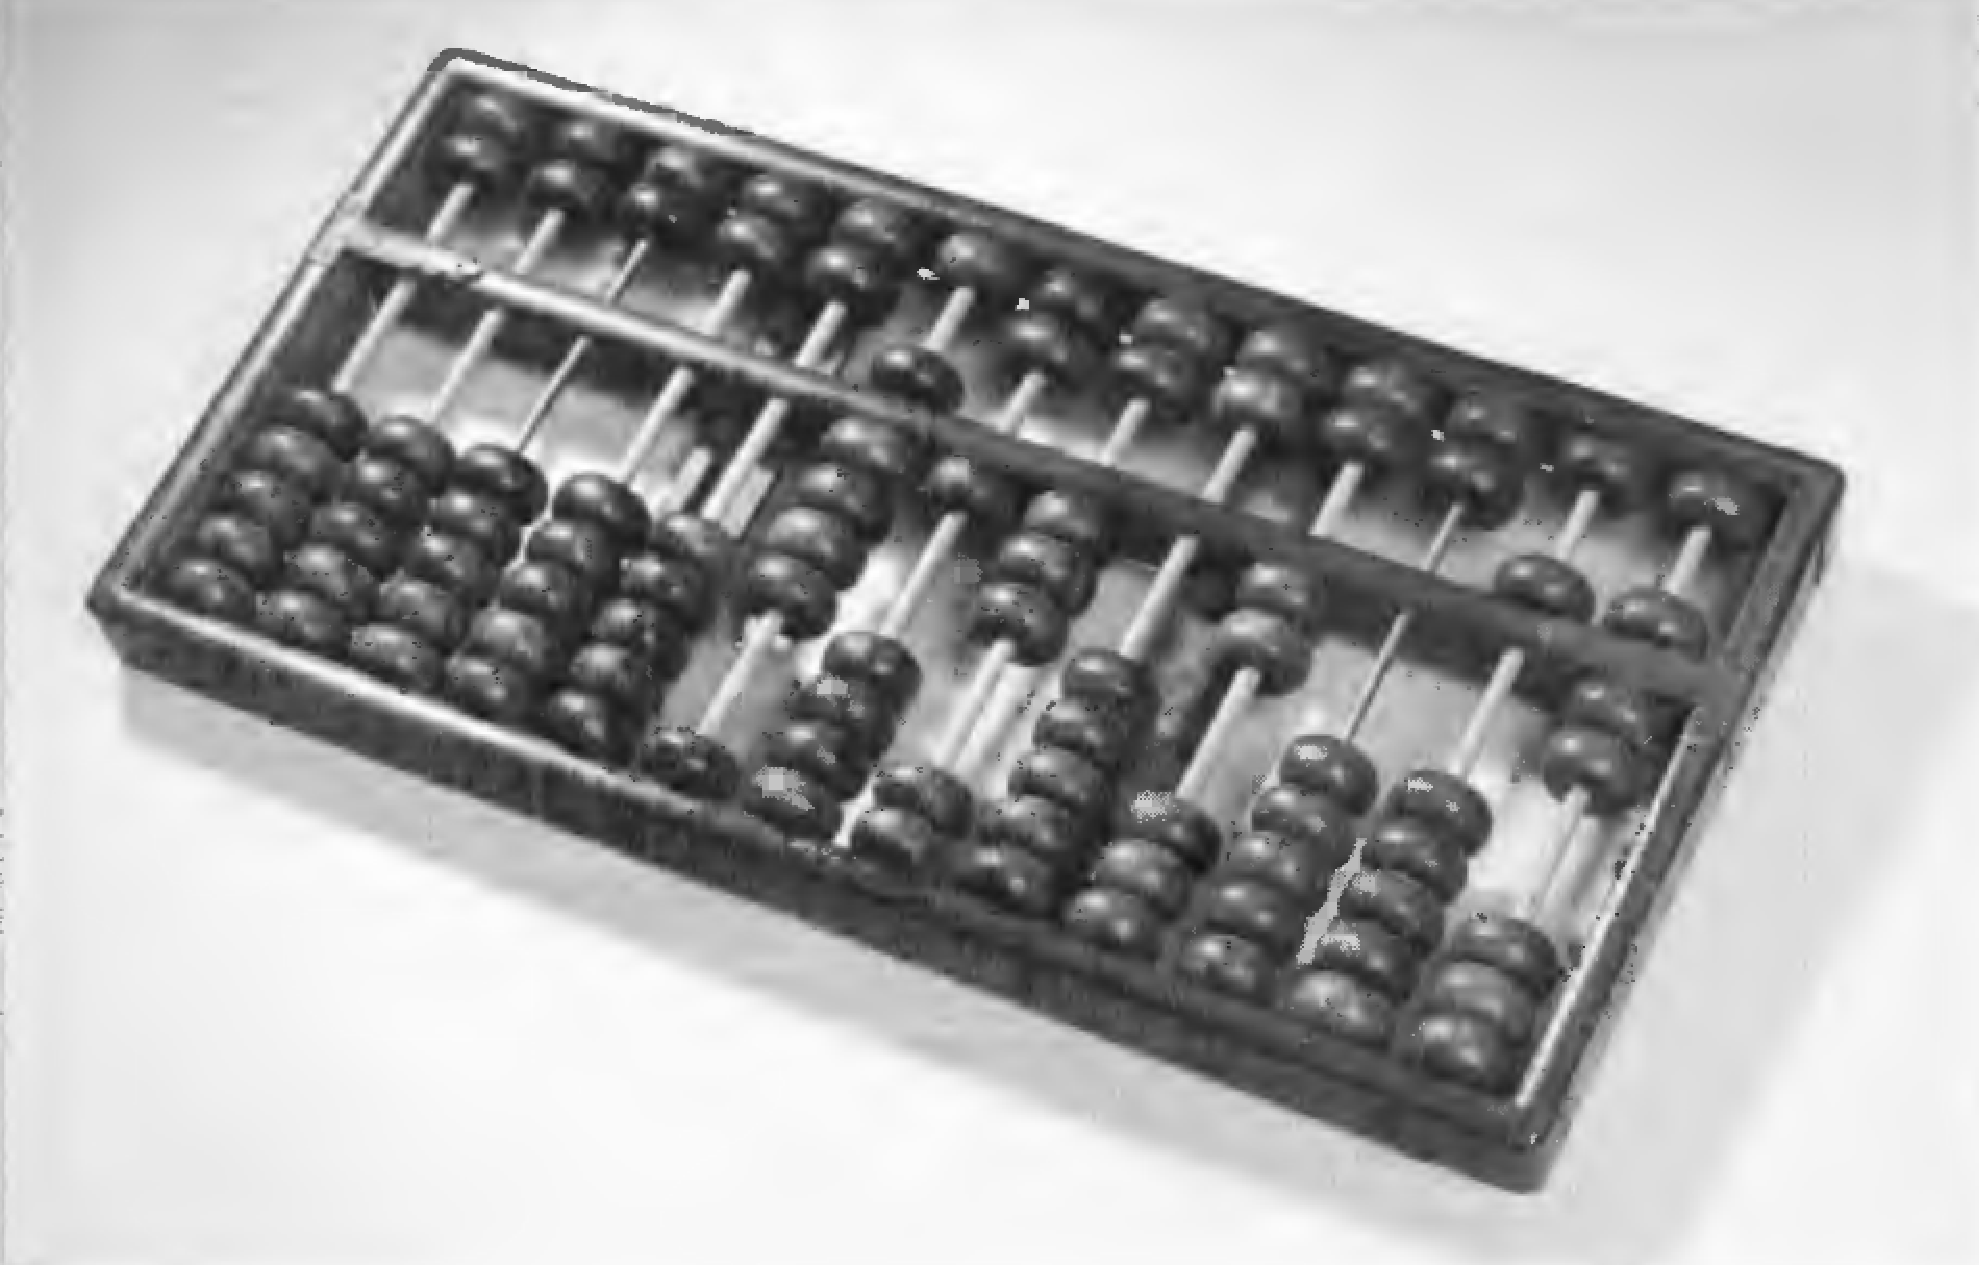
\includegraphics{ch0/fig03.pdf}}
\caption{Một bàn tính (ảnh chụp bởi Wayne Chandler)}
  \label{fig:fig0.3}
\end{figure}
 


Gần đây hơn, các thiết kế của máy tính đã dựa trên công nghệ cơ học. Một số nhà phát minh
trong thời kỳ này là Blaise Pascal (1623-1662) của Pháp, Wilhelm Gottfried Leibniz
(1646-1716) của Đức, và Charles Babbage (1792-1871) của Anh. Những máy này biểu diễn dữ
liệu thông qua vị trí của bánh răng, với các dữ liệu đầu vào được đặt một cách cơ học bằng
vị trí ban đầu của bánh răng.  Đầu ra của các máy của Pascal và của Leibniz đã được xác
định bằng cách quan sát các vị trí của bánh răng khi việc thực hiện kết thúc. Để tránh các sai sót khi ghi lại kết quả tính toán, 
Babbage đã thiết kế máy cho phép in luôn kết quả tính toán ra giấy.


Ta có thể thấy các máy ngày càng linh hoạt hơn (theo nghĩa làm việc theo thuật toán). Máy
của Pascal chỉ thực hiện phép cộng đơn giản bằng cách đặt một dãy các bước thích hợp ngay
trong bản thân cấu trúc của máy. Tương tự, máy của Leibniz có thuật toán được nhúng sẵn
vào trong kiến trúc của nó, mặc dù nó đã cho phép người dùng thao tác để lựa chọn trong
nhiều phép toán số học. Máy tính sai phân của Babbage (Babbage's Difference Engine), thực
ra nó vẫn chỉ là mô hình trên giấy, có thể thay đổi thực hiện nhiều phép toán phong phú;
và máy Phân tích (Analytical Engine), máy mà Babbage chưa bao giờ nhận được tài trợ để
làm, đã được thiết kế để đọc các lệnh dưới dạng các lỗ trên thẻ giấy. Bởi vậy máy Phân
tích của Babbage là có thể lập trình được. Trên thực tế, Augusta Ada Byron (Ada Lovelace)
đã xuất bản một bài báo chỉ ra cách lập trình trên máy Phân tích để thực hiện nhiều tính
toán. Và ngày nay người ta vẫn xem Ada như lập trình viên đầu tiên trên thế giới.


Ý tưởng biểu diễn các thuật toán thông qua giấy đục lỗ không phải bắt đầu từ Babbage. Ông
đã dựa trên ý tưởng trước đó của Joseph~Jacquard (1752-1834). Vào năm 1801,
Joseph Jacquard đã tạo nên một khung dệt, mà trong đó từng bước của quá trình dệt đã được
xác định bởi các mẫu lỗ đục trên thẻ giấy. Theo cách này, các thuật toán được thực hiện
bởi các khung dệt có thể thay đổi một cách dễ dàng theo các thiết kế mẫu dệt khác
nhau. Herman Hollerith (1860-1929) cũng đã sử dụng ý tưởng của Jacquard để tăng tốc độ xử
lý các bảng tính trong điều tra số dân của Mỹ năm 1890. Kiểu thẻ này sau đó đã được gọi là
thẻ đục lỗ đã là một phương tiện giao tiếp với máy tính rất phổ biến vào những năm
1970s. Cho đến nay các kỹ thuật này vẫn được sử dụng, như trong cuộc bầu cử tổng thống Mỹ
năm 2000.

Do hạn chế về công nghệ, việc sản xuất các máy cơ học phức tạp của của Pascal, Leibniz, và
Babbage thời đó rất tốn kém. Nhưng với những tiến bộ trong công nghệ điện tử vào đầu năm
1900, trở ngại này đã được khắc phục. Ví dụ như máy điện của George Stibitz, hoàn thành
trong 1940 tại phòng thí nghiệm Bell, và máy Mark I, hoàn thành năm 1944 tại Đại học
Harvard bởi Howard Aiken và một nhóm kỹ sư của IBM (Hình \ref{fig:fig0.4}). Nhưng các máy
này dùng các rơle cơ học điện tử, trong khi các nhà nghiên cứu khác đã áp dụng các kỹ
thuật ống chân không, nên chúng đã bị lỗi thời ngay sau khi được xây dựng. Một trong những
chiếc máy đầu tiên sử dụng công nghệ ống chân không là máy Atanasoff-Berry do John
Atanasoff và trợ lý của mình là Clifford Berry xây dựng trong thời kỳ từ 1937 đến 1941 tại
Iowa State College (nay là Đại học bang Iowa). Một máy khác được gọi là Colossus, đã được
xây dựng dưới sự chỉ đạo của Tommy Flower ở Anh để giải mã các bức điện bằng Tiếng Đức
trong Thế chiến thứ II (World War II). (Trên thực tế, người ta đã làm khoảng mười chiếc
máy. Nhưng vì lý do bí mật quân sự và an ninh quốc gia nên người ta đã không công bố, do
đó những chiếc máy này không trở thành một phần trong ``cây phả hệ của họ máy tính''.)
Sau đó, đã có các máy linh hoạt hơn, như ENIAC (Electronic Numerical Intergrator and
Calculator) được phát triển bởi John Mauchly và J. Presper Eckert tại Trường Moore thuộc
khoa Công nghệ Điện tử, Đại học Pennsylvania.

\begin{figure}[tb]
\centering
    \scalebox{0.5}{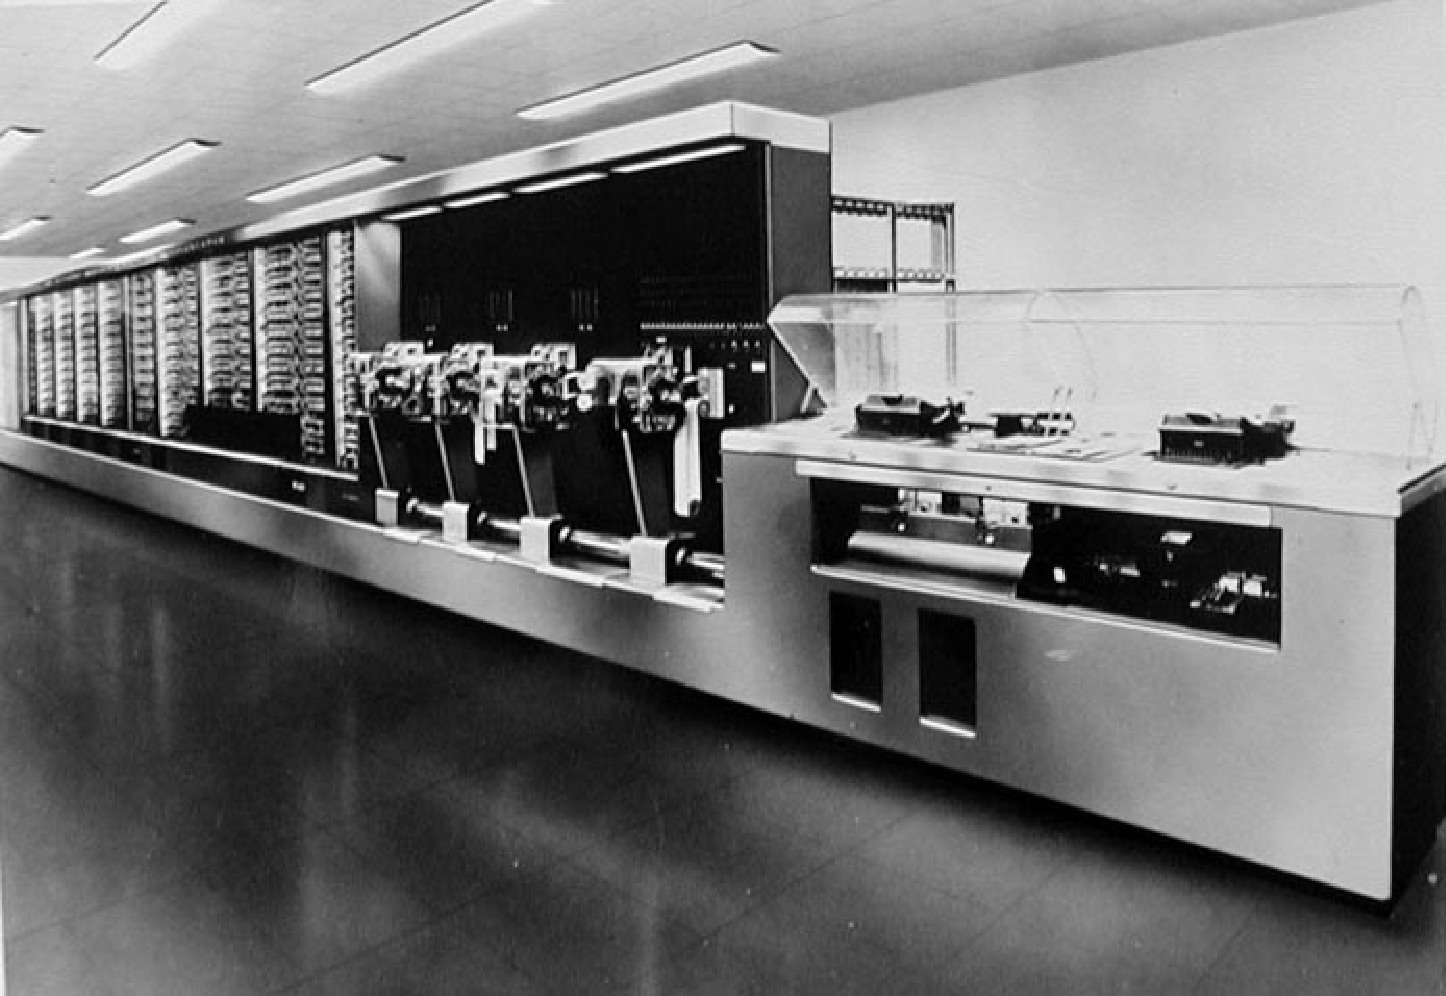
\includegraphics{ch0/fig04.pdf}}
\caption{Máy tính Mark I}
  \label{fig:fig0.4}
\end{figure}


Từ đó đến nay, lịch sử của máy tính gắn liền với việc phát triển công nghệ, bao gồm việc
phát minh ra transitors và sau đó là sự phát triển của các mạch tích hợp, sự xuất hiện
truyền thông qua vệ tinh, và tiến bộ trong công nghệ quang. Ngày nay, một chiếc máy tính
nhỏ cầm tay có thể có hiệu suất tính toán lớn hơn so với máy tính kích thước bằng cả căn
phòng của những năm 1940 và có thể trao đổi thông tin nhanh chóng qua qua hệ thống truyền
thông toàn cầu.

Một bước quan trọng làm cho máy tính trở nên phổ biến là sự phát triển của máy tính để
bàn~(desktop computer).  Những máy này bắt nguồn từ những người ưa thích máy tính, họ bắt
đầu thử tự làm các máy tính tại nhà ngay sau khi có những chiếc máy tính dùng trong nghiên
cứu vào những năm 1940. Cũng chính vì ham thích, Steve Jobs và Stephen Wozniak đã tạo ra
chiếc máy tính dùng ở nhà có thể thương mại được, và đến năm 1976, họ đã thành lập Apple
Computer, Inc, để sản xuất và bán các sản phẩm của họ. Các công ty khác cũng có các sản
phẩm tương tự trên thị trường là Commodore, Heathkit, và Radio shack. Mặc dù các sản phẩm
này rất được những người yêu thích máy tính ưa chuộng, chúng lại không được giới doanh
nhân chấp nhận. Và chính những doanh nhân này đã tìm đến công ty IBM để sản xuất đại trà
phục vụ nhu cầu tính toán của họ.

Năm 1981, IBM giới thiệu chiếc máy tính để bàn đầu tiên, nó được gọi là máy tính cá nhân
hay máy PC (Personal Computer). Các phần mềm cơ bản bên trong nó được phát triển bởi một
công ty mới thành lập là Microsoft. Máy PC đã thành công một cách nhanh chóng và được thừa
nhận rộng rãi trong giới doanh nhân. Ngày nay, thuật ngữ PC được sử dụng rộng rãi để chỉ
tất cả những máy (từ nhiều nhà sản xuất khác nhau) được phát triển từ máy tính để bàn của
IBM và hầu hết trong số chúng được bán kèm với các phần mềm của Microsoft. Tuy nhiên, đôi
khi thuật ngữ PC cũng được dùng chung cho cả \textit{máy tính để bàn (desktops)} hoặc
\textit{máy tính xách tay~(laptops)}.

Việc thu nhỏ kích thước của máy tính và các phát triển các tính năng của chúng đã đưa
ngành công nghệ máy tính trở thành ngành công nghệ đi đầu trong xã hội. Ngày nay, công
nghệ máy tính trở nên phổ biến đến mức việc trang bị các kiến thức về nó đã trở thành một
yêu cầu tối thiểu để hoà nhập với xã hội hiện đại. Máy tính gia đình đang được tích hợp
với các hệ thống truyền thông và giải trí. Các máy điện thoại di động và máy ảnh kỹ thuật
số bây giờ được kết hợp lại trong một thiết bị cầm tay được gọi là PDA (Personal Digital
Assistants).

Trên phạm vi rộng, công nghệ máy tính làm đã thay đổi cách điều hành của chính phủ, đã có
những tác động rất lớn đến nền kinh tế toàn cầu, dẫn đến những tiến bộ lớn lao trong
nghiên cứu khoa học. Ta khó có thể tưởng tượng được điều gì sẽ đến trong tương lai.


%%% Local Variables: 
%%% mode: latex
%%% TeX-master: "../tindaicuong"
%%% End: 

\section{Khoa học thuật toán}
Thuở ban đầu, do khả năng lưu trữ thông tin bị giới hạn và các thủ tục lập trình dài dòng,
rắc rối nên các thuật toán được sử dụng trong các máy tính toán còn rất đơn giản. Theo
thời gian, các rào cản này dần bị phá bỏ; các máy đã được ứng dụng cho các nhiệm vụ lớn
hơn và phức tạp hơn. Việc biểu diễn các nhiệm vụ phức tạp này dưới dạng thuật toán đã bắt
đầu thách thức khả năng của con người. Chính vì vậy, ngày càng có nhiều nghiên cứu hướng
về thuật toán và lập trình.

Trong bối cảnh này, các kết quả lý thuyết của các nhà toán học mới bắt
đầu mới thể hiện tầm quan trọng của nó. Nhờ định lý về tính không toàn
vẹn của G\"odel, các nhà toán học đã bắt đầu nghiên cứu các vấn đề
liên quan đến thuật toán nảy sinh từ công nghệ cao. Từ đây, nổi lên
một nghành khoa học mới, gọi là \textit{khoa học máy tính}.

Ngày nay, khoa học máy tính cũng được coi như là như là khoa học thuật
toán. Phạm vi của ngành khoa học này rất rộng, liên quan đến cả toán
học, kỹ thuật, tâm lý học, sinh học, quản trị kinh doanh, và ngôn ngữ
học. Trong các chương tiếp theo, ta sẽ thảo luận nhiều vấn đề
khác nhau của ngành khoa học này. Với mỗi vấn đề, mục tiêu của chúng
ta bao gồm: giới thiệu các ý tưởng trung tâm, các vấn đề đang được
nghiên cứu, và một vài phương pháp đang được sử dụng để phát triển tri
thức trong lĩnh vực này.

Để có được một bức tranh tổng thể về khoa học máy tính, ta xem
xét những câu hỏi sau đây:

\begin{figure}[tb] 
\centering
    \scalebox{0.4}{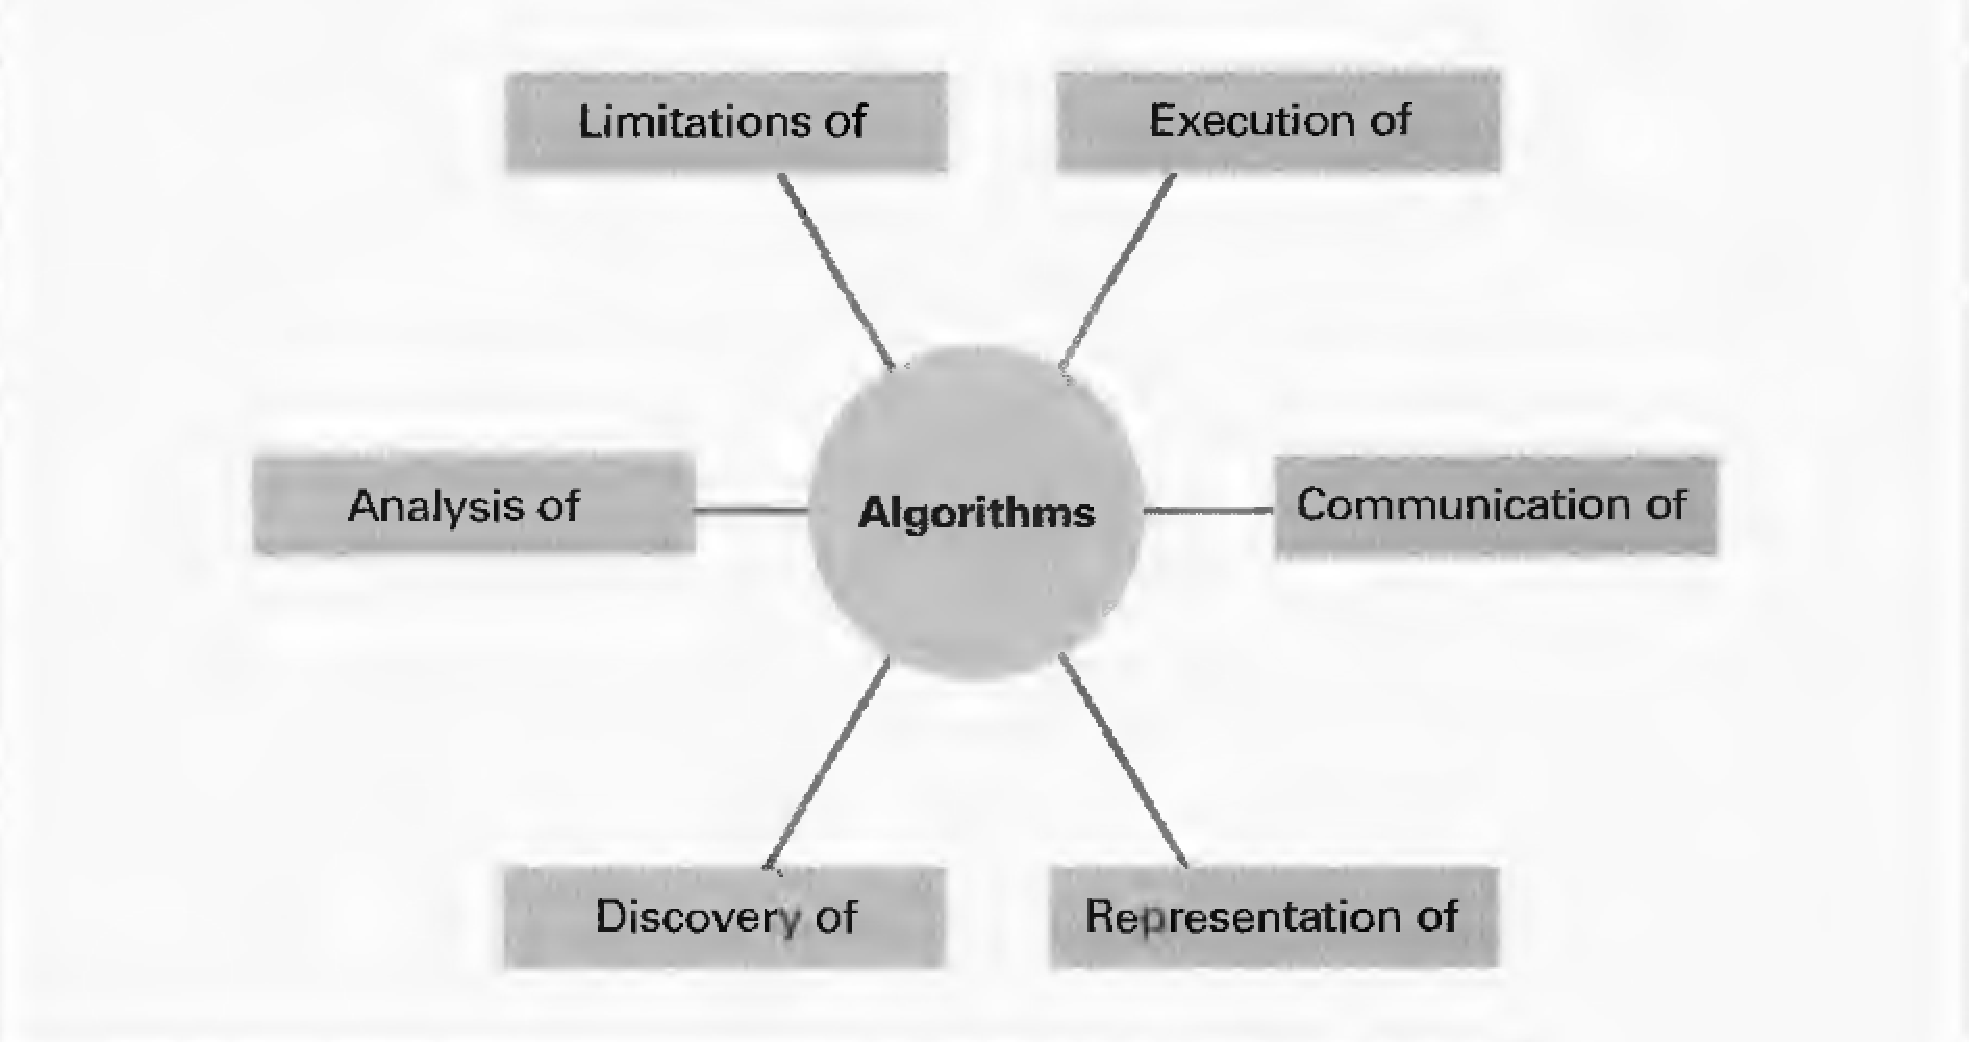
\includegraphics{ch0/fig05.pdf}}
\caption{Vai trò trung tâm của thuật toán trong khoa học máy tính}
  \label{fig:fig0.5}
\end{figure}

\begin{itemize}
\item Những bài toán nào có thể được giải bằng thuật toán?

\item Làm sao để có thể phát hiện ra thuật toán một cách dễ dàng hơn?

\item Làm sao để biểu diễn và truyền tải thuật toán một cách tốt
  hơn?

\item Làm sao để các kiến thức về thuật toán giúp ta tạo ra
  các máy tốt hơn?

\item Làm sao để có thể phân tích và so sánh các đặc trưng 
  của các thuật toán khác nhau?
\end{itemize}

Chú ý rằng các câu hỏi này đều hướng đến một chủ đề chung là nghiên
cứu thuật toán~(Hình~\ref{fig:fig0.5})




%%% Local Variables: 
%%% mode: latex
%%% TeX-master: "../tindaicuong"
%%% End: 

\section{Khái niệm trừu tượng}
 
Bởi vì khái niệm trừu tượng được sử dụng rất nhiều trong khoa học máy tính và thiết kế hệ
thống máy tính nên ta cần phải hiểu khái niệm đó ngay từ trong chương mở đầu này. Thuật
ngữ \textbf{trừu tượng}~(abstraction) ở đây nhằm chỉ sự phân biệt giữa tính chất bên ngoài
của một đối tượng và chi tiết hình thành bên trong của đối tượng đó. Nhờ trừu tượng mà ta
có thể bỏ qua chi tiết bên trong của các thiết bị phức tạp như máy tính, ô-tô, hoặc lò
vi-ba sóng; thay vào đó chỉ cần nắm bắt được các giao diện chức năng để sử dụng.  Hơn nữa,
nhờ công cụ trừu tượng nên người ta mới xây dựng được những hệ thống phức tạp.  Máy tính,
ôtô, và các lò vi-ba sóng được tạo nên từ các thành phần, mỗi thành phần lại được xây dựng
từ các thành phần nhỏ hơn. Mỗi thành phần biểu diễn một mức trừu tượng. Ở mỗi mức trừu
tượng, ta sử dụng lại các thành phần mức thấp hơn mà không phải quan tâm chi tiết xem
chúng hình thành thế nào.

Nhờ có trừu tượng, ta có thể xây dựng, phân tích, và quản lý các hệ thống máy tính lớn,
phức tạp. Các hệ thống này rất rắc rối nếu nhìn các đối tượng của chúng một cách chi
tiết. Theo từng mức trừu tượng, ta chỉ nhìn hệ thống dưới dạng các thành phần, gọi là các
\textbf{công cụ trừu tượng} (abstract tools), mà bỏ qua chi tiết về cấu thành bên trong
của chúng. Điều này cho phép ta tập trung xem xét xem các thành phần (ở cùng mức) tương
tác với nhau như thế nào và làm thế nào để tập hợp chúng lại thành một thành phần ở mức
cao hơn. Bởi vậy, ta có thể hiểu từng phần của hệ thống.

Ta nhấn mạnh rằng việc trừu tượng không chỉ giới hạn trong phạm vi khoa học và công
nghệ. Nó là kỹ thuật đơn giản hoá quan trọng tạo ra lối sống của xã hội. Rất ít người
trong chúng ta hiểu sự tiện lợi trong cuộc hàng ngày được thực hiện như thế nào-- ta ăn và
mặc những thứ mà bản thân ta không thể làm ra được, ta sử dụng các thiết bị điện mà không
cần phải hiểu về công nghệ chế tạo ra nó. Ta sử dụng các dịch vụ của những người khác mà
không cần biết một cách chi tiết về nghề của họ. Từng bước, người ta cố gắng chuyên biệt
cách thực hiện một số thứ trong xã hội, còn những người khác chỉ cần cố gắng tìm hiểu để
sử dụng các kết quả đó như là công cụ trừu tượng. Theo cách này, kho các công cụ trừu
tượng của xã hội được mở rộng, và khả năng của xã hội không ngừng tiến xa hơn.

Ta còn gặp lại chủ đề trừu tượng nhiều lần trong nghiên cứu. Ta sẽ thấy rằng các thiết bị
máy tính được xây dựng ở mức của các công cụ trừu tượng.  Sự phát triển của các hệ thống
phần mềm lớn là theo cách mô đun hoá trong đó mỗi mô đun được sử dụng như là một công cụ
trừu tượng trong mô đun lớn hơn. Hơn nữa, trừu tượng đóng vai trò quan trọng trong nhiệm
vụ phát triển ngành khoa học máy tính, cho phép các các nhà nghiên cứu hướng sự chú ý tới
các lĩnh vực đặc biệt bên trong một lĩnh vực phức tạp. Trên thực tế, cách tổ chức của cuốn
sách này phản ánh đặc trưng của khoa học. Mỗi chương trọng tâm vào một chủ đề cụ thể,
chương này độc lập với chương khác, nhưng khi ghép lại cùng nhau nó trở thành một tài liệu
tổng quan dễ hiểu về các lĩnh vực rộng được nghiên cứu.

%%% Local Variables: 
%%% mode: latex
%%% TeX-master: "../tindaicuong"
%%% End: 

  
%%% Local Variables: 
%%% mode: latex
%%% TeX-master: "../tindaicuong"
%%% End: 

\chapter{Lưu trữ dữ liệu}
\label{chap:chuong1}
\minitoc 
\vspace{0.5cm}
\noindent
Trong chương này, ta sẽ xem xét cách dữ liệu được biểu diễn và lưu trữ trong máy tính.  Cụ
thể, ta sẽ xem xét cách biểu diễn văn bản, giá trị số, âm thanh, hình ảnh và video. Nhiều
thông tin trong chương này cũng thích hợp với các lĩnh vực khác như ảnh số, sản xuất và
thu âm audio/video, và truyền thông khoảng cách xa.

  
\section{Các bít và cách lưu trữ}

Máy tính thực chất là một máy điện, nó hoạt động dựa theo nguyên tắc lựa chọn tắt hoặc mở
hàng triệu chuyển mạch rất nhỏ bên trong nó. Các trạng thái tắt hoặc bật này được mã hoá
dưới dạng các số $0$ hoặc $1$. Các số này được gọi là các bít (gọi tắt của \textit{số nhị
  phân}).


Thông tin trong máy tính được biểu diễn dưới dạng dưới dạng dãy bít~0 hoặc~1, và dù rằng
ta nhìn các bít như giá trị số thì chúng thực sự vẫn chỉ là ký hiệu hình thức, ý nghĩa của
nó tuỳ thuộc từng cách áp dụng--lúc chúng được dùng để biển diễn giá trị số, lúc chúng
được dùng để biểu diễn ký tự trên một bảng chữ nào đó, lúc này chúng là biểu diễn hình
ảnh, lúc khác lại là biểu diễn âm thanh.

\subsection*{Phép toán Boolean}

Nếu ta xem bít $0$ biểu diễn một giá trị logic \textit{false} và bít $1$ biểu diễn cho giá
trị \textit{true} thì các thao tác bên trong máy tính có thể được mô tả một cách hình thức
bởi các \textbf{phép toán Boolean}, theo tên của George~Boole (1815-1864), một người đi
tiên phong trong Logic toán. Hình  \ref{fig:op-bool1} liệt kê ba trong nhiều phép toán
boolean: AND, OR, XOR. Các phép toán này về mặt hình thức tương tự như các phép toán hai
ngôi Nhân, Cộng và Trừ trong số học, chúng cũng nhận hai tham số đầu vào và trả ra kết
quả. Ví dụ, phép toán AND với đầu vào là cặp giá trị false~($0$) và true~($1$) sẽ cho kết
quả là false~($0$); cụ thể ta có:
\[
  0 \AND 1 = 0.
\] 
Khác ba phép toán đề cập ở trên, phép toán $\NOT$ là phép toán một ngôi, nó chỉ có một đầu
vào và một đầu ra. Trong đó đầu ra là giá trị đảo của đầu vào:
\[
\NOT  0 = 1 \mbox{ và } \NOT 1 = 0.
\]

\begin{figure}[tb]
\centering
  \begin{minipage}{1.5in}
    \begin{tabular}{cc|c}
      $p$ & $q$ & $p \AND q$ \\
      \hline
      0 & 0 & 0 \\
      0 & 1 & 0 \\
      1 & 0 & 0 \\
      1 & 1 & 1
    \end{tabular}
  \end{minipage}
  \begin{minipage}{1.5in}
    \begin{tabular}{cc|c}
      $p$ & $q$ & $p \OR q$ \\
      \hline
      0 & 0 & 0 \\
      0 & 1 & 1 \\
      1 & 0 & 1 \\
      1 & 1 & 1
    \end{tabular}
  \end{minipage}
  \begin{minipage}{1.5in}
    \begin{tabular}{cc|c}
      $p$ & $q$ & $p \XOR q$ \\
      \hline
      0 & 0 & 0 \\
      0 & 1 & 1 \\
      1 & 0 & 1 \\
      1 & 1 & 0
    \end{tabular}
  \end{minipage}
  \caption{Các phép toán AND, OR, XOR (tuyển loại). Hai cột đầu tiên biểu diễn tham số đầu
    vào, cột thứ ba chỉ kết quả của phép toán tương ứng với tham số đó.}
    \label{fig:op-bool1}
\end{figure}

\subsection*{Các cổng logic và Flip-Flop} 

%Các kết quả của đại số Boolean rất quan trọng trong thiết kế các thành phần của máy tính. Ý tưởng cơ bản là xây dựng các mạch đơn giản thực hiện một vài phép toán Boolean, còn các mạch phức tạp hơn có thể xây dựng lại được bằng cách kết hợp các mạch đơn giản đó.

\begin{figure}[tbh]  
\centering

\subfloat[Cổng logic $\AND$]{
  \begin{minipage}{3in}
\begin{center}
    \scalebox{0.5}{
\includegraphics{ch2/fig2and.pdf}}

    \vspace{0.5cm}
    \begin{tabular}{cc|c}
      \multicolumn{2}{c|}{Đầu vào} &  Đầu ra \\
      \hline
      0 & 0 & 0 \\
      0 & 1 & 0 \\
      1 & 0 & 0 \\
      1 & 1 & 1
    \end{tabular}
  \end{center}
\end{minipage}
}
\subfloat[Cổng logic $\OR$]{
  \begin{minipage}{3in}
    \begin{center}
      \scalebox{0.5}{
\includegraphics{ch2/fig2or.pdf}} 

      \vspace{0.5cm}
      \begin{tabular}{cc|c}
      \multicolumn{2}{c|}{Đầu vào} &  Đầu ra \\
      \hline
      0 & 0 & 0 \\
      0 & 1 & 1 \\
      1 & 0 & 1 \\
      1 & 1 & 1
    \end{tabular}
  \end{center}
\end{minipage}
}

\vspace{0.7cm}

\subfloat[Cổng logic $\XOR$]{
  \begin{minipage}{3in}
    \begin{center}
      \scalebox{0.5}{
\includegraphics{ch2/fig2xor.pdf}}

      \vspace{0.5cm}
      \begin{tabular}{cc|c}
        \multicolumn{2}{c|}{Đầu vào} &  Đầu ra \\
        \hline
        0 & 0 & 0 \\
        0 & 1 & 1 \\
        1 & 0 & 1 \\
        1 & 1 & 0
      \end{tabular}
    \end{center}
\end{minipage}
}
\subfloat[Cổng logic $\NOT$]{
  \begin{minipage}{3in}
    \begin{center}
      \scalebox{0.5}{
\includegraphics{ch2/fig2not.pdf}} 

\vspace{0.5cm}
      \begin{tabular}{c|c}
        Đầu vào &  Đầu ra \\
        \hline
        0 & 0 \\
        1  & 0 
      \end{tabular}
    \end{center}
  \end{minipage}
} 

\vspace{0.3cm}
\caption{Các cổng logic}
\label{fig:op-bool2}
\end{figure}


\begin{figure}[tbh]  
\centering
    \scalebox{0.4}{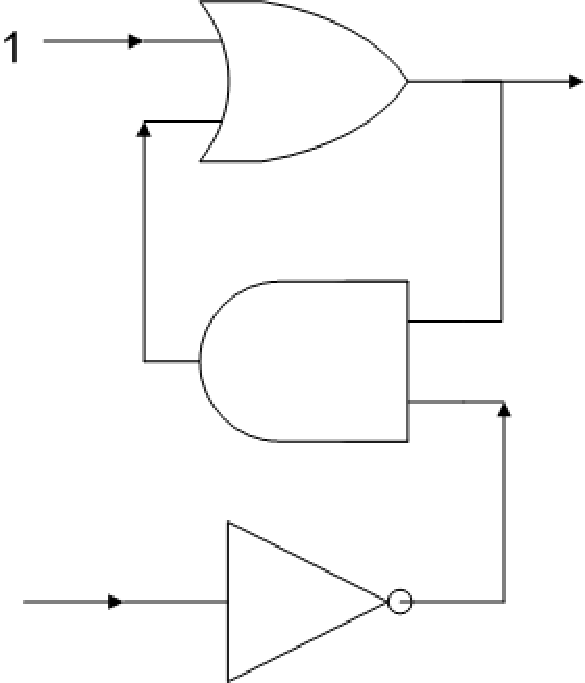
\includegraphics{ch2/fig-fflp.pdf}}
\caption{Một mạch Flip-Flop}
 \label{fig:op-flipflop}
\end{figure}
 

\textbf{Cổng} là một thiết bị điện tử có một hoặc nhiều đầu vào, mỗi đầu vào nhận giá trị
$0$ hoặc~$1$, tương ứng với hai mức điện thế; và thường có một đầu ra, đó là một hàm theo
đầu vào, nó cũng nhận giá trị~$0$ hoặc~$1$.  Trong giáo trình này, ta sẽ chỉ xem xét một
cách hình thức các cổng như các ký hiệu, bỏ qua cách biểu diễn vật lý của chúng.

Một cổng thường để tính toán một hàm Boolean cụ thể, đơn giản nào đó. Trong nghành công
nghiệp điện tử, người ta thường chỉ xây dựng một số cổng thực hiện một vài hàm nhất định,
còn các hàm khác sẽ được xây dựng lại bằng cách tổ hợp các cổng cơ bản đó.  Một số cổng
quen thuộc được liệt kê trong Hình~\ref{fig:op-bool2}.

 
Các cổng được tổ hợp thành các \textbf{mạch số} (gọi tắt là mạch) bằng cách nối đầu ra của
một số cổng với đầu vào một số cổng khác. Mỗi mạch có thể có một hoặc nhiều đầu vào, mỗi
đầu vào này lại có thể là đầu vào của nhiều cổng khác bên trong mạch. Đầu ra của mạch là đầu ra của một hoặc
nhiều cổng trong mạch.

Một mạch quan trọng trong thiết kế các phần tử nhớ được chỉ ra trong Hình~\ref{fig:op-flipflop}, nó được gọi là mạch Flip-Flop. Một Flip-Flop là một mạch được thiết
kế để giữ giá trị đầu ra ($0$ hoặc~$1$) không thay đổi cho tới khi nhận được tín hiệu từ
đầu vào yêu cầu chuyển sang một giá trị khác. Để ý rằng, khác với các phép toán Boolean
trước, giá trị đầu ra của mạch kiểu này không chỉ phụ thuộc đầu vào ở thời điểm hiện tại
mà còn phụ thuộc cả vào đầu ra của thời điểm trước nữa.

Ta khẳng định rằng: khi cả hai giá trị đầu vào của mạch trong Hình \ref{fig:op-flipflop}
đều là~$0$ thì đầu ra của mạch không thay đổi (dù nó có là $0$ hay $1$). Tuy nhiên, khi ta
đặt giá trị $1$ cho đầu vào phía trên của mạch, ngay lập tức đầu ra sẽ là~$1$. Còn khi ta
đặt giá trị $1$ cho đầu vào phía dưới, ngay lập tức đầu ra của mạch sẽ là $0$.


\begin{figure}[tbh] 
\centering
\subfloat[Đặt $1$ và $0$ vào 2 đầu vào]{
    \scalebox{0.35}{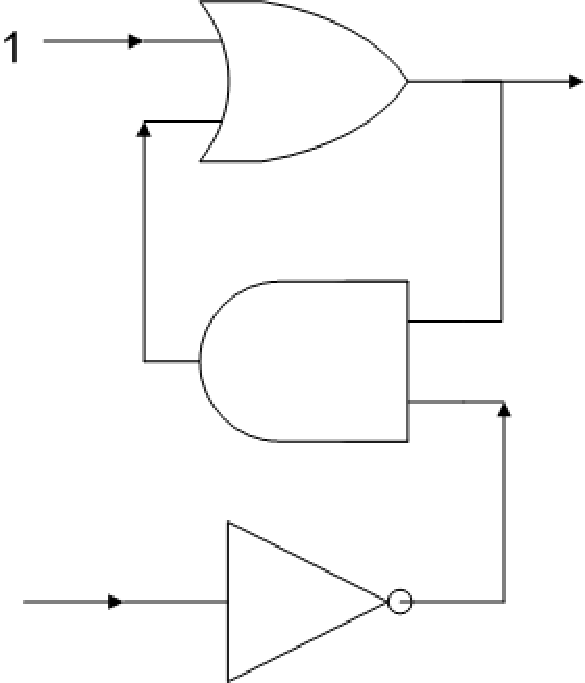
\includegraphics{ch2/figffl1.pdf}}
\label{op-flipflop2a}
}\qquad \subfloat[Đầu ra của cổng $\OR$ và cổng $\AND$ đều là $1$]{
  \scalebox{0.35}{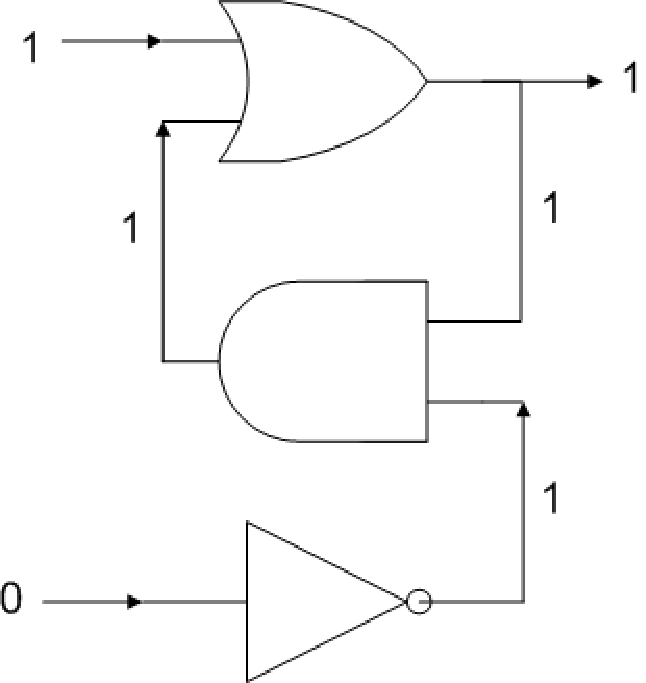
\includegraphics{ch2/figffl2.pdf}}
\label{op-flipflop2b}
} \qquad \subfloat[Giá trị $1$ từ cổng $\AND$ giữ cho đầu ra của $\OR$
bằng $1$ dù đầu vào kia bằng $0$]{
  \scalebox{0.35}{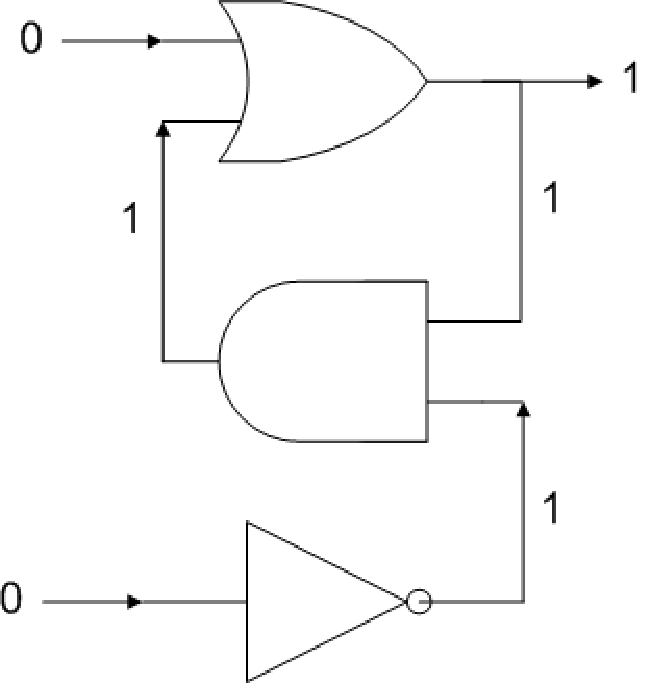
\includegraphics{ch2/figffl3.pdf}}
\label{op-flipflop2c}
}
\caption{Đưa giá trị đầu ra của Flip-Flop lên 1}
\label{fig:op-flipflop2}
\end{figure}

Ta sẽ cùng phân tích khẳng định trên một cách chi tiết. Trước hết, ta thấy rằng dù đầu ra
của mạch~\ref{fig:op-flipflop} là gì đi nữa, nếu đầu vào phía trên của mạch đặt
bằng~$1$ và phía dưới đặt bằng $0$, vậy đầu ra của cổng $\OR$ sẽ là~$1$. Bây giờ, cả hai
đầu vào của cổng $\AND$ đều bằng $1$, vậy đầu ra của nó bằng $1$, có nghĩa rằng đầu vào
thứ hai của $\OR$ sẽ là~$1$ (Hình~\ref{op-flipflop2b}). Điều này làm cho đầu ra của $\OR$
vẫn bằng $1$, kể cả khi bây giờ đầu vào phía trên của mạch được đặt bằng $0$ (Hình~\ref{op-flipflop2c}).  Tóm lại, đầu ra của Flip-Flop đã trở thành $1$ và luôn giữ ở giá
trị đó dù đầu vào phía trên được đặt bằng $0$ hay không.
 

Cũng tương tự như trên, khi đặt giá trị $1$ cho đầu vào phía dưới sẽ làm cho đầu ra của
Flip-Flop là $0$ và giá trị này vẫn giữ nguyên khi giá trị đầu vào được đưa trở về~$0$.
   
Ta trình bày mạch Flip-Flop trong Hình~\ref{fig:op-flipflop} và Hình~\ref{fig:op-flipflop2}
với hai mục đích. Thứ nhất, nó chỉ ra làm thế nào các thiết bị có thể được xây dựng từ
các cổng, quá trình này được gọi là thiết kế mạch số, nó đóng vai trò quan trọng trong
nghành công nghệ máy tính. Thứ hai, nó cho ta cách để lưu trữ một bít trong máy tính. Thật
vậy, mạch Flip-Flop cho phép ta đặt giá trị để đầu ra của nó luôn bằng $0$ hoặc bằng
$1$. Vậy các mạch khác muốn lưu trữ có thể gửi tín hiệu tới đầu vào của Flip-Flop để đặt
giá trị, và các mạch khác nữa có thể sử dụng giá trị lưu trữ bằng cách lấy giá trị từ đầu
ra của Flip-Flop như đầu vào của nó. Với kỹ thuật hiện nay, rất nhiều Flip-Flop có thể
được kết hợp lại trong một chip và được sử dụng để lưu trữ thông tin dưới dạng mã hoá như
dãy bít~$0$ và~$1$.

\subsection*{Bài tập}
\begin{enumerate}
 \item Với những giá trị đầu vào nào thì mạch sau đây cho đầu ra là $1$?
    \begin{center}
      \scalebox{0.55}{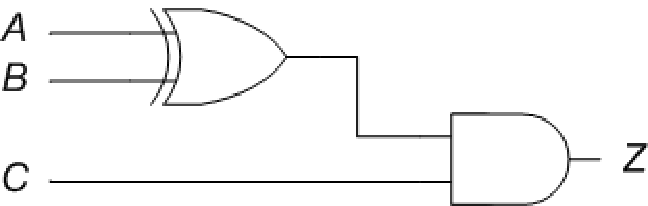
\includegraphics{ch2/bt1.pdf}}
    \end{center}

 \item Phần trình bày ở trên khẳng định rằng việc đặt $1$ cho đầu vào
   phía dưới của Flip-Flop trong Hình~\ref{fig:op-flipflop} (trong khi
   vẫn giữ đầu vào phía trên bằng $0$) sẽ làm cho đầu ra của Flip-Flop
   bằng $0$. Hãy mô tả dãy các sự kiện xuất hiện trong Flip-Flop trong
   trường hợp này?

  \item Một cách xây dựng Flip-Flop khác được chỉ ra bởi hình dưới đây. Giả sử rằng cả hai
    đầu vào của Flip-Flop này là $0$, hãy mô tả dãy các sự kiện xuất hiện khi cho đầu vào
    phía trên giá trị $1$.
   \begin{center}
     \scalebox{0.6}{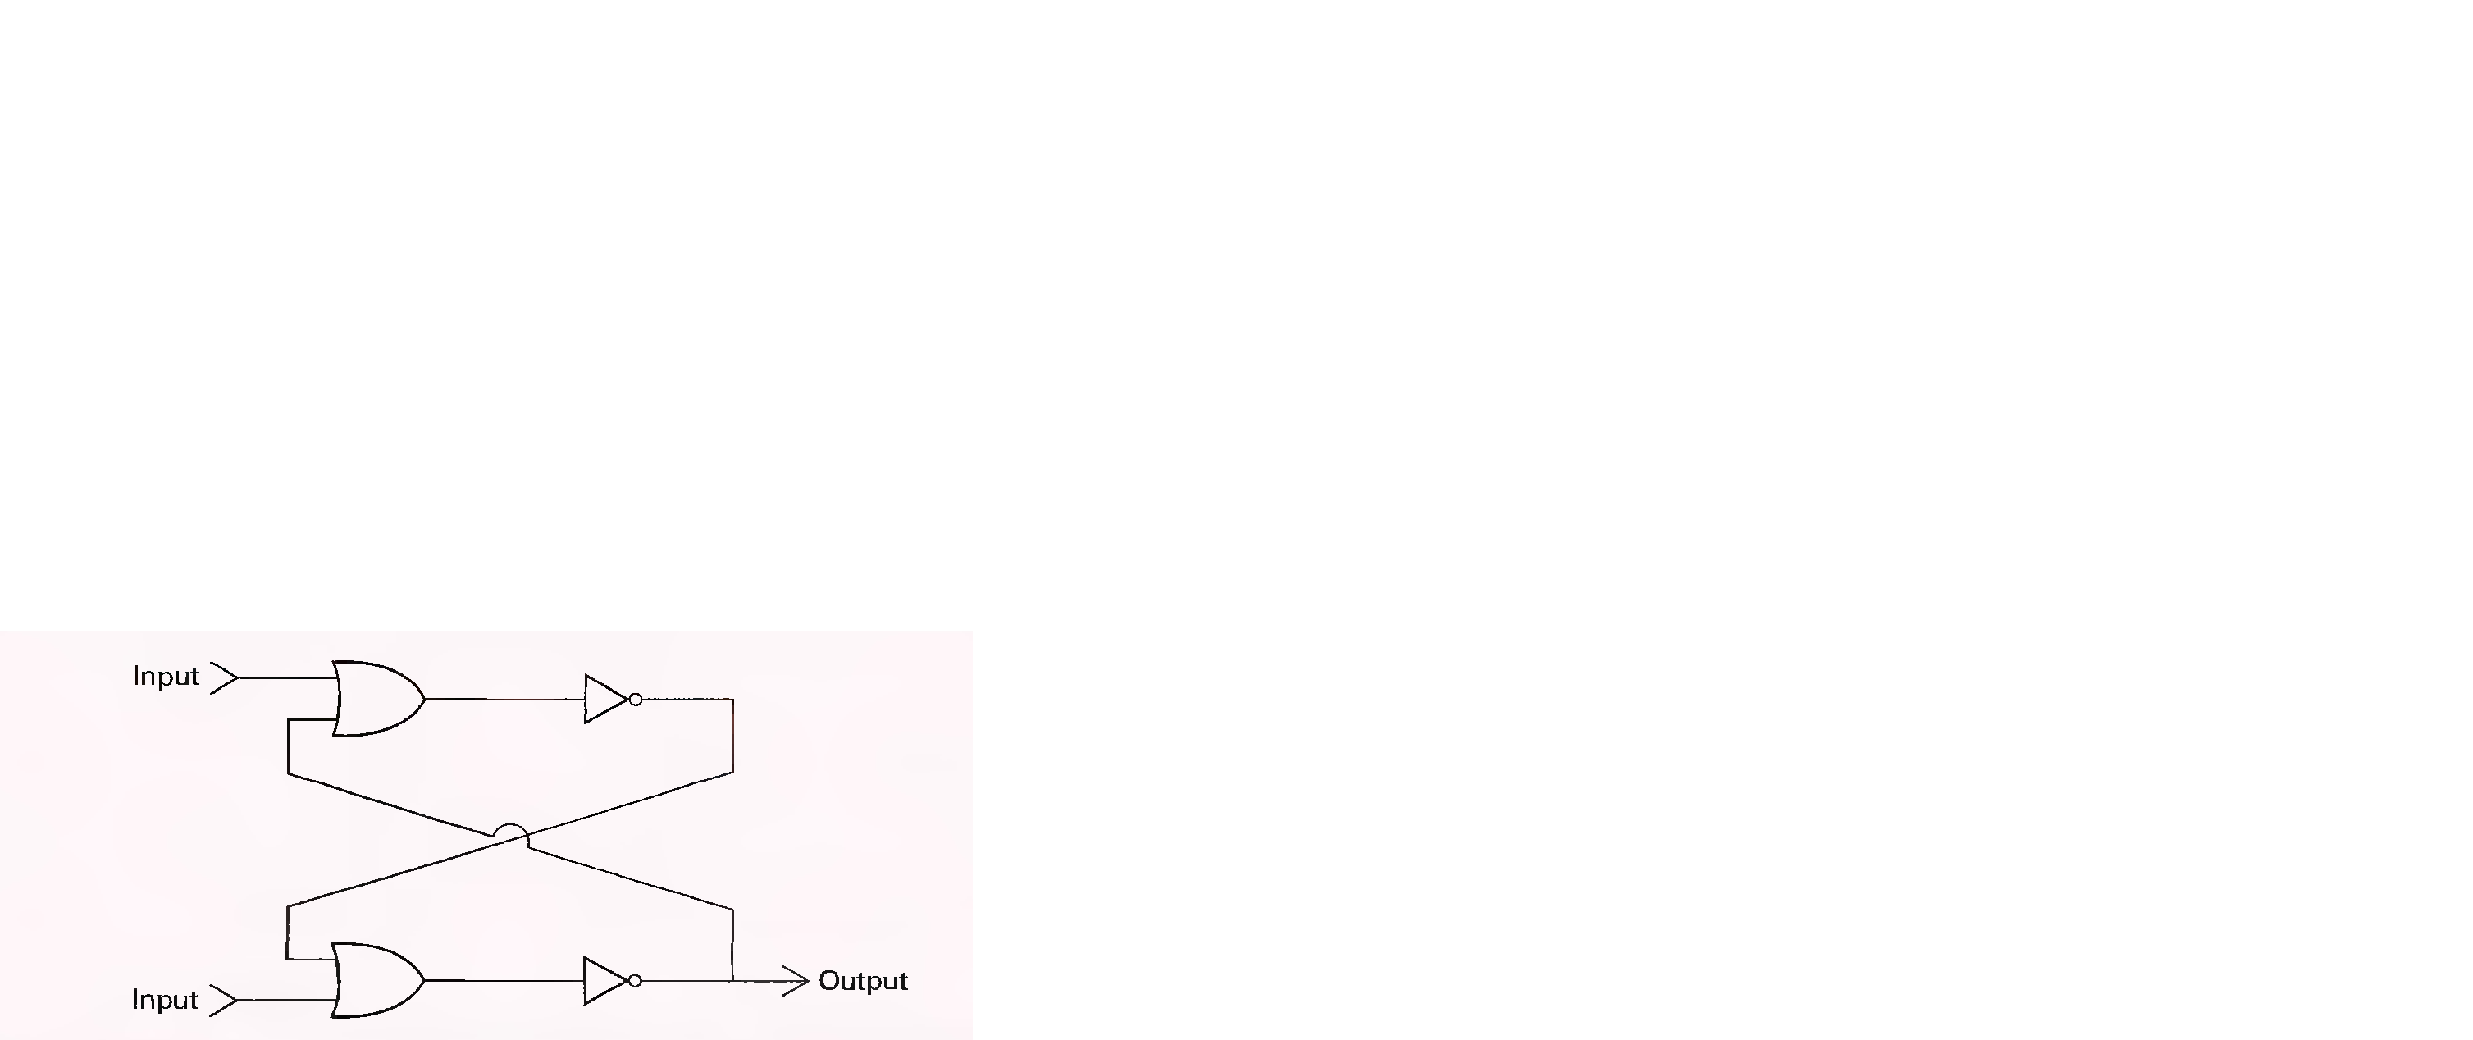
\includegraphics{ch2/fig15.pdf}}
   \end{center}


 \item Phối hợp các hoạt động của các thành phần khác nhau bên trong
   máy tính là rất cần thiết. Điều này được làm bằng cách nối với một
   xung đồng hồ với các mạch cần phối hợp.  Bởi vì đồng hồ thay đổi
   luân phiên giữa giá trị $0$ và $1$, nó làm cho các thành phần mạch
   hoạt động. Dưới đây là một ví dụ một phần của mạch liên quan đến
   Flip-Flop trong Hình~\ref{fig:op-flipflop}. Giá trị nào của xung
   đồng hồ sẽ chặn các giá trị đầu vào của mạch tác động đến
   Flip-Flop? Giá trị nào của xung đồng hồ sẽ làm cho Flip-Flop phản
   ứng lại với giá trị đầu vào của mạch?
    \begin{center}
      \scalebox{0.55}{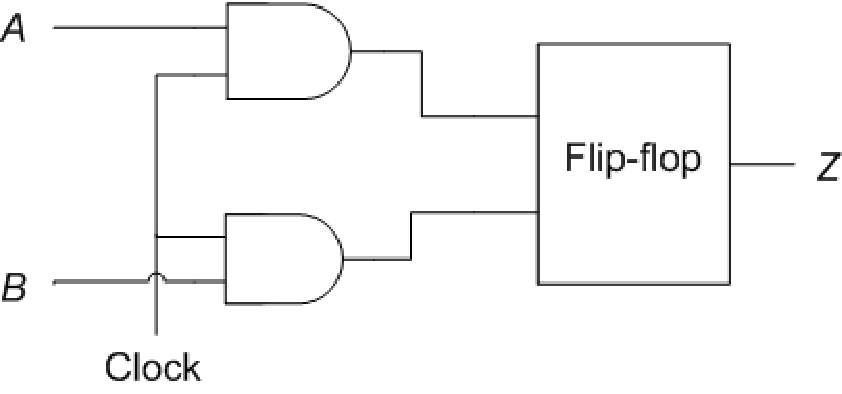
\includegraphics{ch2/bt4.pdf}}
    \end{center}

\item
  \begin{enumerate}
  \item Nếu đầu ra của cổng $\OR$ được nối với cổng $\NOT$, ta gọi nó
    là mạch $\NOR$. Mạch này có đầu ra là $1$ chỉ khi cả hai đầu vào
    đều có giá trị $0$. Ta ký hiệu cổng này cũng giống cổng $\OR$
    nhưng thêm một vòng tròn ở đầu ra của nó. Mạch dưới đây bao gồm
    một cổng $\AND$ và hai cổng $\NOR$. Hãy mô tả phép toán Boolean mà
    mạch này tính?
%\begin{figure}[h]
    \begin{center}
      \scalebox{0.55}{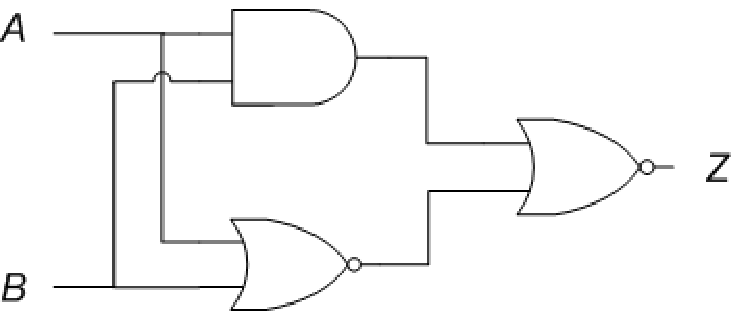
\includegraphics{ch2/bt5a.pdf}}
    \end{center}
%\caption{Một mạch Flip-Flop}
%  \label{fig:op-flipflop}
%\end{figure}

  \item Nếu đầu ra của cổng $\AND$ được nối với cổng $\NOT$, ta gọi nó
    là mạch $\NAND$.  Mạch này có đầu ra là $0$ chỉ khi cả hai đầu vào
    đều có giá trị $1$. Ta ký hiệu cổng này cũng giống cổng $\AND$
    nhưng thêm một vòng tròn ở đầu ra của nó. Mạch dưới đây bao gồm
    các cổng $\NAND$. Hãy mô tả phép toán Boolean mà mạch này tính?
    \begin{center}
      \scalebox{0.55}{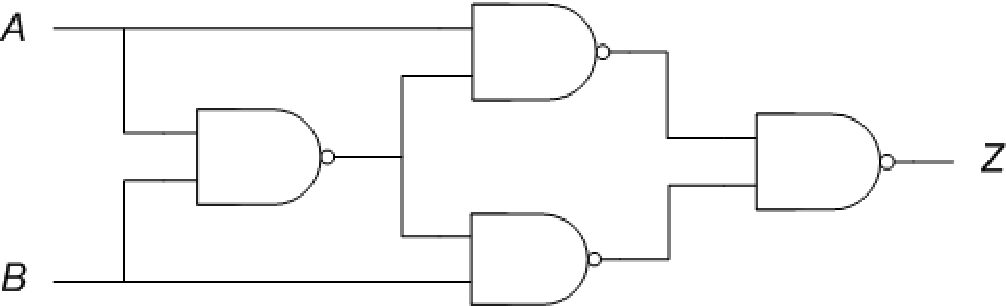
\includegraphics{ch2/bt5b.pdf}}
    \end{center}

  \end{enumerate}
\end{enumerate}

%%% Local Variables: 
%%% mode: latex
%%% TeX-master: "../tindaicuong"
%%% End: 
   
\section{Bộ nhớ chính}

Để lưu trữ dữ liệu, một máy tính chứa một tập các mạch (kiểu như Flip-Flops), mỗi mạch có
khả năng lưu trữ một bít. Dãy bít này gọi là \textbf{bộ nhớ chính} của máy.

\subsection*{Tổ chức bộ nhớ}
Bộ nhớ chính của máy tính được tổ chức theo các đơn vị dễ quản lý, gọi là các \textbf{ô
  nhớ}, một ô nhớ thường gồm tám bít (hay là một \textbf{byte}). Với các máy tính nhỏ dùng
cho các thiết bị gia đình như lò vi sóng, bộ nhớ chính của nó có thể chỉ gồm vài nghìn ô
nhớ. Trong khi các máy tính lớn có thể có bộ nhớ chính lên tới hàng tỷ ô nhớ.

Các ô nhớ trong máy tính không có thứ tự. Tuy nhiên, ta vẫn thường quy ước sắp xếp chúng
theo hàng. Phía phải nhất của hàng này được gọi là ở vị trí \textbf{cao} và phía trái được
gọi là vị trí \textbf{thấp}. Mỗi vị trí (byte) của hàng ta lại đánh thứ tự tính từ
\textit{phải qua trái}. Bít phía trái nhất có trọng số cao nhất và cũng thường được gọi là
\textbf{bít dấu} (cách gọi này dựa theo cách biểu diễn giá trị số của ô nhớ.).  Ta có thể
biểu diễn nội dung của ô nhớ với kích thước tính theo byte như theo Hình~\ref{fig:fig1.8}.

\begin{figure}[tb]
\centering
    \scalebox{0.4}{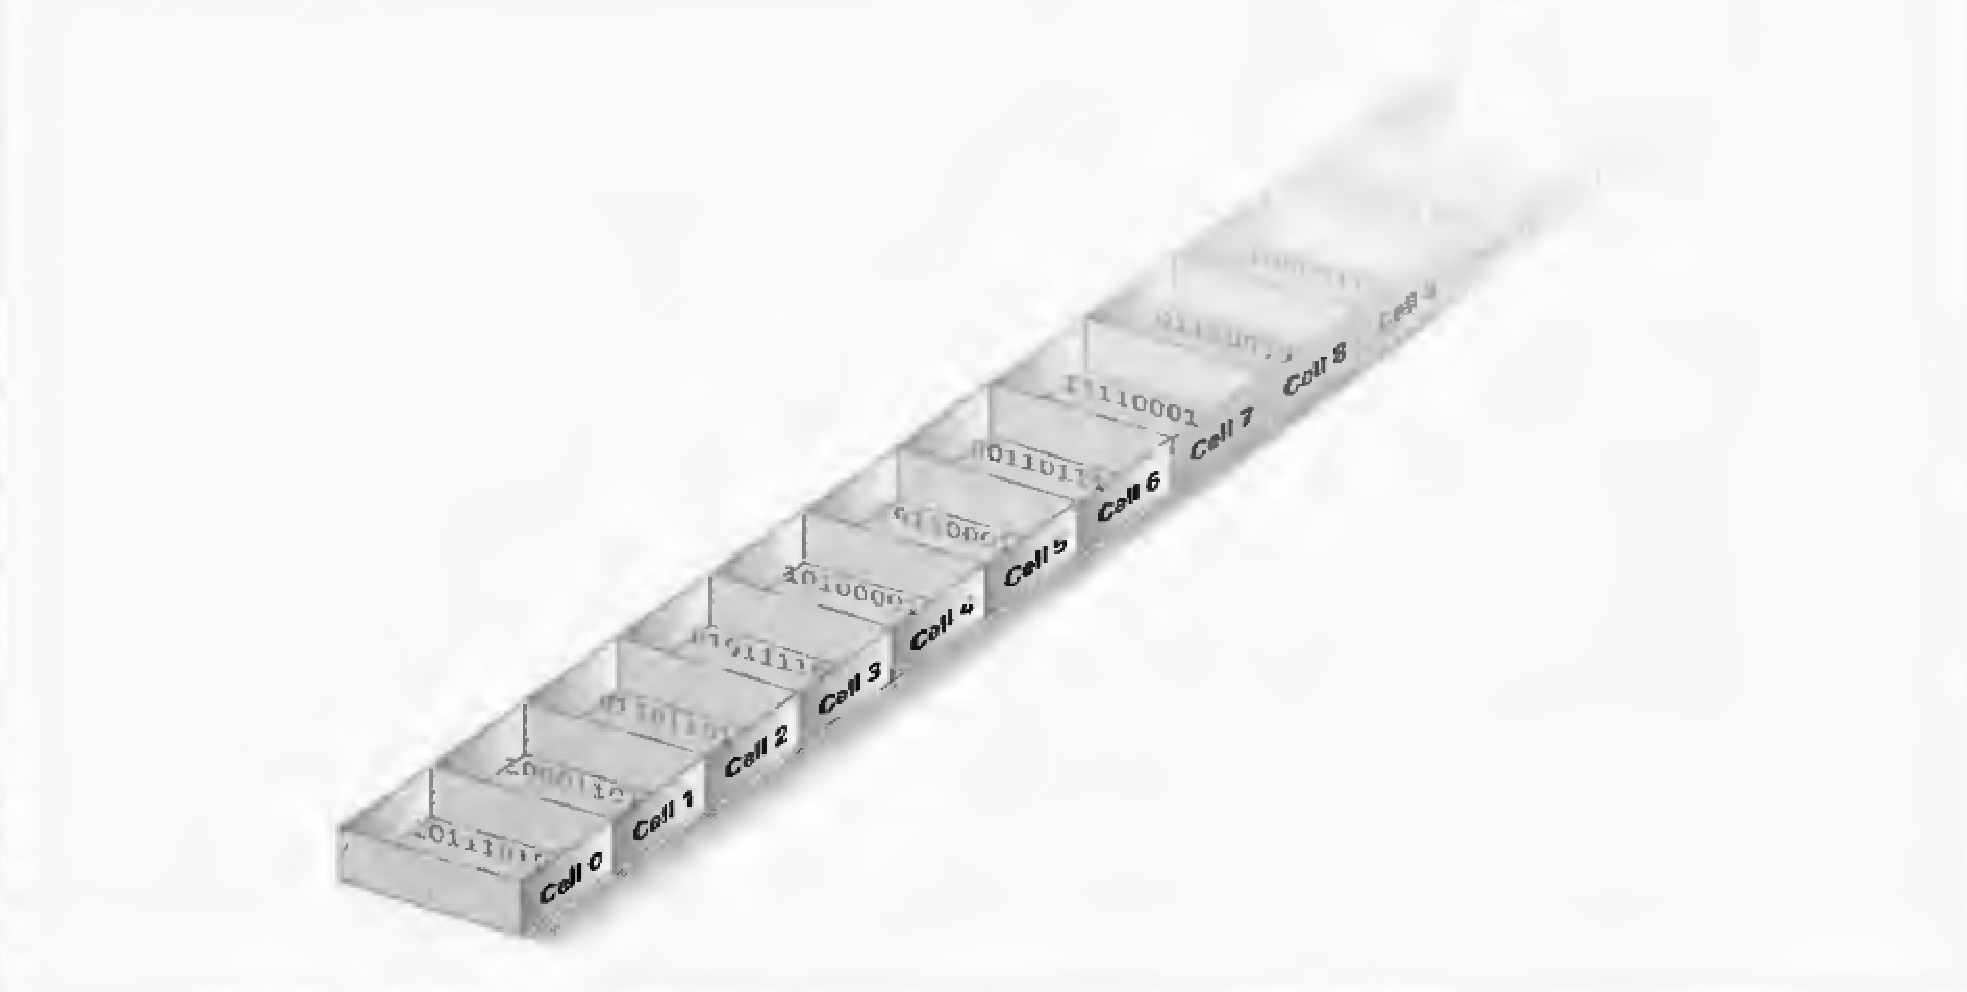
\includegraphics{ch2/Fig1-8.pdf}}
\caption{Các ô nhớ được sắp xếp theo địa chỉ}
  \label{fig:fig1.8}
\end{figure}

Để xác định ô nhớ trong bộ nhớ chính, mỗi ô nhớ được gán với một ``tên'' duy nhất, được
gọi là \textbf{địa chỉ}. Phương pháp này tương tự với cách đánh địa chỉ nhà trong thành
phố. Chính xác hơn, ta nhìn các ô nhớ xếp theo hàng và đánh số bắt đầu từ $0$. Cách đánh
địa chỉ kiểu này cho ta cách xác định ô nhớ một cách duy nhất. Tuy vậy, nó cũng gắn cho
các ô nhớ một thứ tự (Hình \ref{fig:fig1.8}), thứ tự này cho phép ta sử dụng các thuật ngữ ``ô
nhớ tiếp theo''  hoặc thuật ngữ ``ô nhớ trước''.


Việc gán thứ tự cho các ô nhớ trong bộ nhớ chính và các bít bên trong mỗi ô nhớ cho phép
ta đánh thứ tự các bít của  bộ nhớ chính theo hàng. Vậy ta có thể lưu trữ các
dãy bít có kích thước lớn hơn kích thước  của một ô nhớ. Ví dụ, ta có thể lưu trữ các xâu $16$ bít bằng hai ô nhớ liên tiếp.

% Để bổ trợ cho bộ nhớ chính, các mạch thực sự lưu trữ các bít được tổ
% hợp với mạch được yêu cầu để cho phép mạch lưu trữ và lấy dữ liệu từ
% các ô nhớ. Theo cách này, các mạch khác có thể lấy dữ liệu từ bộ nhớ
% bằng cách hỏi nội dung của một số ô nhớ (được gọi là thao tác đọc bộ
% nhớ), hoặc chúng có thể ghi thông tin vào trong bộ nhớ bằng cách yêu
% cầu một số bít đặt trong ô nhớ tại địa chỉ đặc biệt (được gọi là phép
% toán ghi).
%[.....]

Bởi vì bộ nhớ chính của máy tính được tổ chức như tập các ô nhớ riêng biệt được địa chỉ
hoá, nên các ô nhớ này có thể được truy cập một cách độc lập theo yêu cầu (cách truy cập
này của bộ nhớ chính ngược lại với cách truy cập của thiết bị lưu trữ khối, là thiết bị
trong đó các xâu bít dài được xử lý theo từng  khối). Để mô tả khả năng có thể
truy nhập được vào mọi ô nhớ, bộ nhớ chính được gọi là \textbf{bộ nhớ truy cập ngẫu nhiên
  (RAM)}.

Ta đã giới thiệu các Flip-Flop để lưu trữ các bít, nhưng trên thực tế bộ nhớ RAM trong
các máy tính hiện đại thường được xây dựng theo kỹ thuật khác. Kỹ thuật này cho phép bộ
nhớ có kích thước nhỏ hơn và có thời gian trả lời nhanh hơn. Thông thường, người ta dùng các  mạch điện nhỏ dễ  bị mất điện tích để lưu trữ các bít. Bởi vậy các thiết
bị này thường cần thêm các mạch, gọi là mạch làm tươi, chịu trách nhiệm nạp điện nhiều
lần một giây.

Để đoán nhận việc hay thay đổi này, bộ nhớ máy tính được xây dựng từ kiểu kỹ thuật này gọi là
bộ nhớ động, dẫn tới thuật ngữ \textbf{DRAM} (Dynamic RAM). Hoặc, tại thời điểm viết quyển
sách này, người ta hay nói tới \textbf{SDRAM} (Synchronous DRAM, có nghĩa rằng DRAM có sử
dụng kỹ thuật đồng bộ (Synchronous) làm giảm thời gian cần thiết để lấy nội dung của một ô
nhớ.)

\subsection*{Đơn vị đo khả năng bộ nhớ}
Ta sẽ thấy trong chương tiếp theo rằng việc thiết kế hệ thống bộ nhớ chính trong đó tổng
số ô nhớ là một luỹ thừa của $2$ có rất nhiều điểm tiện lợi. Kích thước của bộ nhớ trước
đây thường được tính theo $1024$ (bằng $2^{10}$) đơn vị ô nhớ. Bởi vì $1024$ là gần với
giá trị $1000$, người ta thường sử dụng tiền tố \textit{kilo} cho đơn vị này. Có nghĩa
rằng, thuật ngữ \textit{kilobyte} (viết tắt là KB) được sử dụng để chỉ $1024$ byte. Bởi
vậy, một máy với $4096$ ô nhớ được gọi là có $4$KB bộ nhớ ($4096 = 4 \times 1024$). Khi bộ
nhớ trở nên lớn hơn, thuật ngữ này được phát triển thêm bao gồm các tiền tố \textit{mega}
cho $1,048,576$ (bằng $2^{20}$) và \textit{giga} cho $1,073,741,824$ (bằng $2^{30}$), và
đơn vị như MB (megabyte) và GB (gigabyte) trở nên phổ biến.

Không may, việc áp dụng các tiền tố thể hiện đơn vị tính có thể gây nhầm lẫn vì các tiền
tố này đã được sử dụng trong các lĩnh vực khác theo đơn vị đo là luỹ thừa của~$10$. Ví dụ,
khi tính khoảng cách, một \textit{kilo-mét} tương ứng bằng $1000$ mét, và khi đo tần xuất
radio, một \textit{mega-hertz} tương ứng bằng $1,000,000$ hertz. Tình huống còn tệ hơn khi
một số nhà sản xuất thiết bị máy tính còn pha trộn hai kiểu thuật ngữ này, dùng KB để
chỉ~$1024$ byte nhưng MB theo nghĩa là $1000$KB (bằng $1,024,000$ byte). Điều này gây lộn
xộn và không rõ ràng cho người dùng thuật ngữ này.

Để làm rõ ràng, người ta đề nghị dùng tiền tố \textit{kilo, mega}, và \textit{giga} cho
các đơn vị theo luỹ thừa của~$10$, và đưa thêm các tiền tố mới \textit{kibi} (viết tắt
kilobinary và ký hiệu là Ki), \textit{mebi} (viết tắt cho megabinary và ký hiệu là Mi), và
\textit{gibi} (viết tắt cho gigabinary và ký hiệu là Gi) tương ứng với đơn vị theo luỹ
thừa của $2$. Với hệ thống này, thuật ngữ \textit{kibibyte} (KiB) có thể để chỉ $1024$
byte, trong khi đó \textit{kilobyte} (KB) dùng để chỉ $1000$ byte. Các thuật ngữ này có
trở thành phổ biến hay không thì phải chờ thời gian trả lời. Hiện tại các thuật ngữ bị
hiểu nhầm \textit{kilo, mega,} và \textit{giga} vẫn bị ăn sâu trong cộng đồng người sử
dụng khi nói tới bộ nhớ chính, bởi vậy ta vẫn theo các ký hiệu truyền thống trong các
nghiên cứu khi tham khảo đến việc lưu trữ dữ liệu. Tuy vậy, các tiền tố \textit{kibi,
  megi}, và \textit{gibi} được đưa ra nhằm giải quyết vấn đề này, và có thể rằng là khôn
ngoan khi diễn dịch các thuật ngữ như \textit{kilobyte} và \textit{megabyte} kèm theo lời
cảnh báo.

\subsection*{Câu hỏi \& Bài tập}
\begin{enumerate}
\item Nếu ô nhớ số $5$ chứa giá trị $8$, hãy chỉ ra sự khác nhau giữa việc viết
  giá trị~$5$ vào ô nhớ số $6$ và chuyển nội dung của ô nhớ số $5$ vào ô nhớ số $6$?

\item Giả sử rằng bạn muốn hoán đổi các giá trị được lưu trữ tại ô nhớ số $2$ cho ô nhớ số
  $3$. Cách thực hiện sau đây có gì sai:
  \begin{description}
  \item \textit{Bước 1.} Chuyển nội dung của ô nhớ số $2$ vào ô nhớ số $3$.
  \item \textit{Bước 2.} Chuyển nội dung của ô nhớ số $3$ vào ô nhớ số $2$.
  \end{description}
  Thiết kế một dãy các bước thực hiện đúng việc tráo đổi nội dung của hai ô nhớ này.

\item Có thể lưu trữ bao nhiêu bít vào bộ nhớ máy tính có dung lượng $4$KB (chính xác hơn
  là KiB)?
  
\end{enumerate}
\section{Thiết bị lưu trữ khối}

Do tính không bền vững và kích thước hạn chế của bộ nhớ chính, nên hầu hết các máy tính
đều có thêm thiết bị nhớ,  gọi là các hệ thống lưu trữ khối (hoặc là lưu trữ thứ
cấp). Các thiết bị này bao gồm đĩa từ, CD, DVD, băng từ, và ổ đĩa flash (ta sẽ thảo luận
các thiết bị này sau). Ưu điểm của hệ thống lưu trữ khối so với bộ nhớ chính là tính lưu
trữ thông tin lâu dài, khả năng lưu trữ lớn, giá thành thấp, và trong nhiều trường hợp cho
ta khả năng có thiết bị lưu trữ tạm thời có thể tách rời khỏi máy.

Thuật ngữ \textit{on-line} và \textit{off-line} thường được sử dụng để mô tả thiết bị được
gắn hoặc tách rời khỏi máy. \textbf{On-line} có nghĩa rằng thiết bị hoặc thông tin được
kết nối và sẵn sàng để đọc từ máy mà không cần sự can thiệp của con
người. \textbf{Off-line} có nghĩa rằng cần sự can thiệp của con người trước khi thiết bị
hoặc thông tin có thể truy cập được từ máy--có thể bởi vì thiết bị phải được bật, hoặc cơ
cấu làm việc yêu cầu các thông tin trung gian phải được thêm vào.

Điểm bất lợi chính của thiết bị lưu trữ khối yêu cầu các dịch chuyển cơ học và bởi thế
chúng cần nhiều thời gian hơn để lưu trữ và nhận dữ liệu từ máy so với bộ nhớ chính, nơi
mà mọi hoạt động đều được thực hiện bằng điện.

\subsection*{Các hệ thống từ tính}


Theo thời gian, các công nghệ từ đang chiếm ưu thế trong lĩnh vực lưu trữ khối. Ví dụ, thiết bị  điển hình được  sử dụng ngày nay là \textbf{đĩa từ}, gồm các đĩa tròn được phủ từ được dùng để lưu trữ dữ liệu. Các đầu đọc/ghi được đặt ở trên và/hoặc dưới đĩa, và khi đĩa xoay tròn,
mỗi đầu đọc đi theo một vòng tròn, gọi là một \textbf{track}, quanh bề mặt bên trên và bên
dưới của đĩa. Bằng cách đặt lại vị trí của đầu đọc/ghi, ta có thể truy cập vào các track đồng tâm khác nhau. Trong nhiều trường hợp, hệ thống lưu trữ bao gồm một vài đĩa được gắn
với một ống suốt chung, đĩa này đặt trên đĩa khác, và khe nhỏ ở giữa hai đĩa đủ đặt các
đầu đọc/ghi. Các đầu đọc/ghi dịch chuyển theo cách thống nhất. Mỗi lần đầu đọc/ghi đặt
lại vị trí, ta lại có một tập mới các track, được gọi là \textbf{cylinder}, có thể truy
cập vào được.

Bởi vì một track thường chứa nhiều thông tin  hơn số thông tin ta muốn xử lý tại một thời điểm,
nên ta lại chia nhỏ mỗi track thành các cung, gọi là \textbf{sector}. Thông tin trên
các sector này được ghi như các xâu bít liên tục (Hình \ref{fig:fig1.9}). Các sector trên
một đĩa có thể có cùng số bít (thông thường là nằm trong khoảng từ $512$ byte tới một
KB). Trong trường hợp đơn giản nhất, hệ thống lưu trữ đĩa có số sector trên mỗi track là
bằng nhau. Vì các track bên ngoài có chu vi lớn hơn so với các track ở bên trong, nên
trong trường hợp này số bít trong một sector trên track ở phía ngoài của đĩa lưu trữ ít
dày đặc hơn so với các track ở gần trung tâm. Trên thực tế, với những hệ thống đĩa có khả
năng lưu trữ cao, các track ở phía ngoài xa trung tâm thường chứa nhiều sector hơn track ở
gần trung tâm. Ta có được khả năng này là nhờ áp dụng một kỹ thuật gọi là
\textbf{zoned-bit recording}. Dùng zone-bit recording, một vài track kề nhau được tập hợp
thành một vùng, các đĩa điển hình chứa khoảng mười vùng. Mọi track trong một vùng có cùng
số sector, nhưng các vùng bên ngoài có nhiều sector trên một track so với vùng bên trong
nó. Theo cách này, không gian lưu trữ của đĩa được sử dụng hiệu quả hơn so với cách của hệ
thống đĩa truyền thống. Nói một cách đơn giản, đây là một hệ thống lưu trữ bao gồm nhiều
sector riêng, mỗi sector có thể được truy cập như một xâu bít độc lập.

\begin{figure}[tb]
\centering
    \scalebox{0.3}{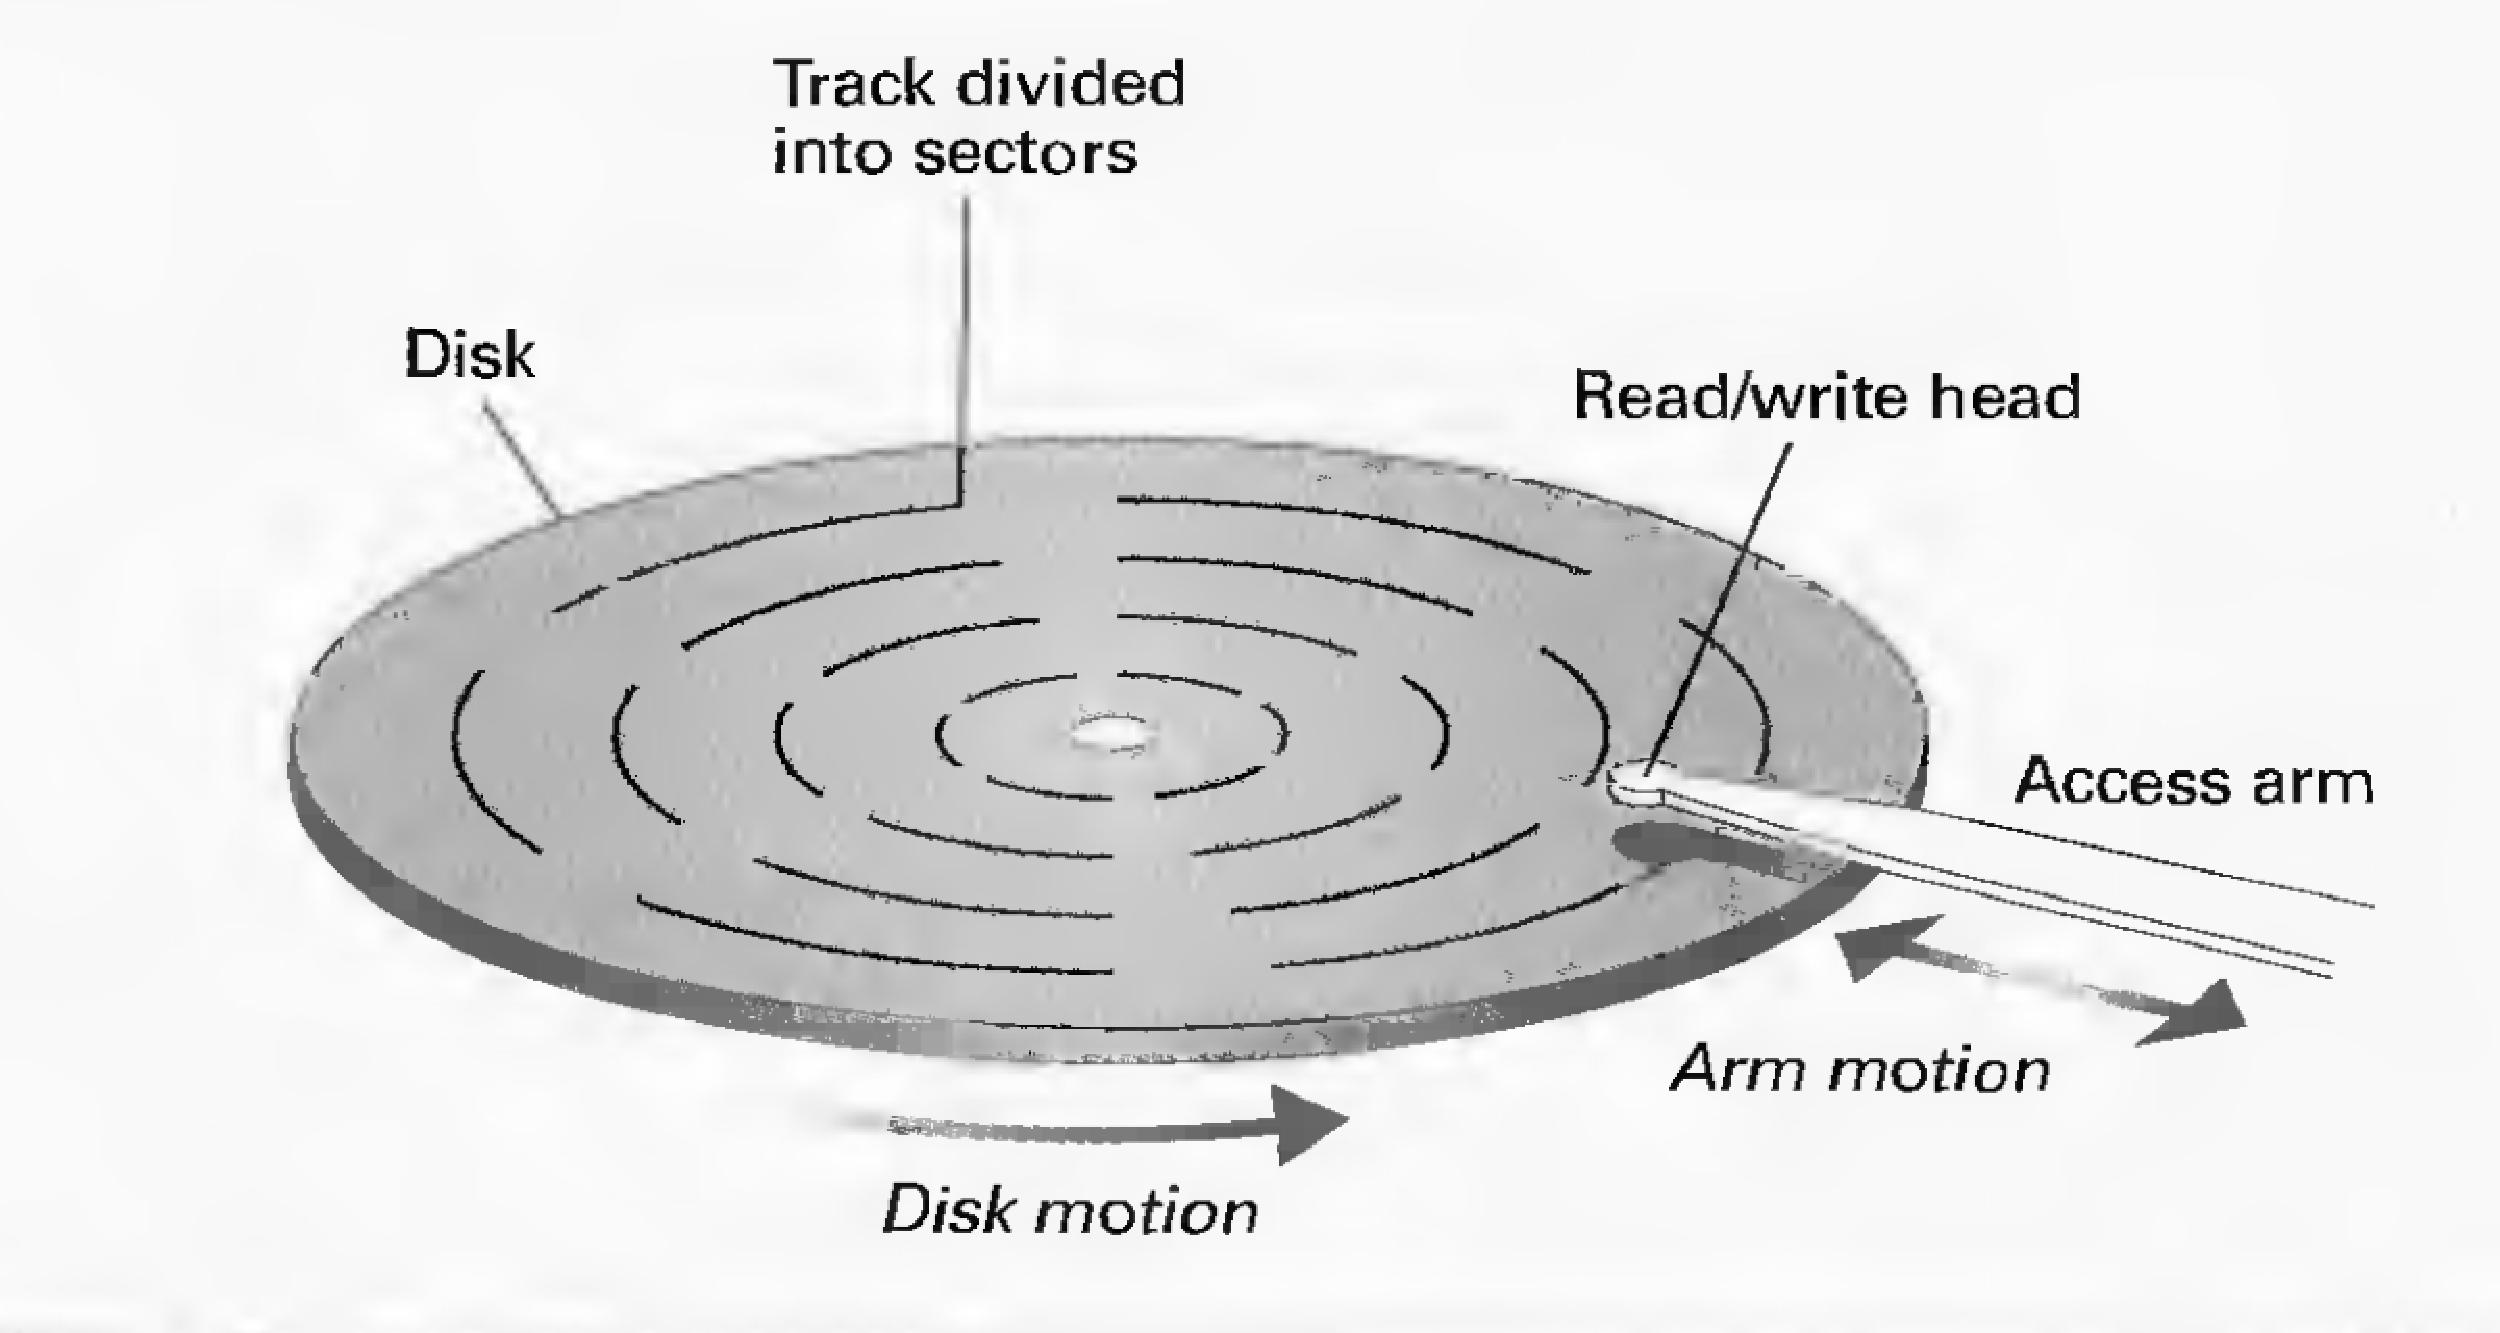
\includegraphics{ch2/Fig1-9.pdf}}
\caption{Một hệ thống lưu trữ đĩa}
  \label{fig:fig1.9}
\end{figure}

Vị trí các track và sector là có thể thay đổi so với cấu trúc vật lý
đĩa. Chúng được đánh dấu về mặt từ tính qua một quá trình gọi là \textbf{formating} (hay
khởi tạo) đĩa. Quá trình này thường được thực hiện bởi nhà sản xuất đĩa, kết quả ta được
một đĩa đã được format. Tuy vậy, hầu hết hệ thống máy tính đều có thể thực hiện nhiệm vụ
này. Bởi vậy, nếu thông tin format trên đĩa bị hỏng, đĩa có thể được format lại. Tuy nhiên
quá trình này sẽ phá huỷ mọi mọi thông tin đã được lưu trữ ghi trên đĩa trước đó.

Khả năng của hệ thống lưu trữ đĩa phụ thuộc vào số đĩa được sử dụng và mật độ track và
sector được thiết đặt. Các hệ thống mức thấp chỉ gồm một đĩa được làm bằng chất dẻo, gọi là \textbf{đĩa mềm}, hay bởi một tên ít dùng hơn là \textbf{floppy}. Đĩa mềm dễ đưa
vào và lấy ra từ các ổ đọc/ghi, đồng thời dễ được lưu trữ lại. Vậy nên đĩa mềm được
dùng rất phổ biến như thiết bị lưu trữ thông tin off-line. Tuy nhiên, bởi vì đĩa
mềm~$3\frac{1}{2}$-in chỉ có khả năng lưu trữ $1.44$MB, nên nó đã nhanh chóng
bị thay thế bởi công nghệ khác.

Các hệ thống đĩa có khả năng lưu trữ cao có thể lưu trữ lên tới nhiều gigabyte. Chúng có
thể bao gồm năm đến mười đĩa cứng đặt trên cùng một trục. Do các đĩa này được làm bằng
chất liệu cứng nên chúng thường được gọi là hệ thống đĩa cứng, ngược lại với thuật ngữ đĩa
mềm. Để cho phép tốc độ quay nhanh, các đầu đọc/ghi trong các hệ thống này không chạm vào
đĩa mà chỉ ``lơ lửng'' trên bề mặt đĩa. Không gian dành cho đầu đọc ở giữa hai đĩa là rất
hẹp, thậm chí chỉ một ít bụi cũng có thể làm kẹt đầu đọc và bề mặt đĩa, dẫn đến phá huỷ cả
hai (hiện tượng này gọi là vỡ đầu đọc). Bởi vậy nên các hệ thống đĩa cứng thường được đặt
bên trong case máy tính và được đóng kín bởi nhà sản xuất.

% Có một vài độ đo để đánh giá hiệu năng hệ thống đĩa:
% \begin{inparaenum}
% \item[(1)] \textbf{thời gian di chuyển} (thời gian chuyển đầu đọc từ track
%   này sang track khác).
% \item[(2)] \textbf{độ trễ vòng quay} hay \textbf{thời gian trễ}
% \end{inparaenum}

%[....]

Hệ thống đĩa cứng nói chung có những đặc trưng tốt hơn so với đĩa mềm. Bởi vì đầu đọc/ghi
không chạm vào bề mặt đĩa, nên nó có tốc độ quay lên tới vài nghìn vòng trong một
phút. Trong khí đó hệ thống đĩa mềm quay chỉ khoảng $300$ vòng một phút. Do đó tốc độ
truyền của hệ thống đĩa cứng, thường là vài MB trên giây, lớn hơn rất nhiều so với đĩa mềm
(chỉ vài KB trên giây).

Do các thao tác của hệ thống đĩa yêu cầu chuyển động về mặt vật lý, nên nó kém hơn rất
nhiều so với tốc độ của mạch điện tử. Thời gian trễ của mạch điện được tính theo đơn vị
nano giây (một phần tỷ của giây) hoặc ít hơn, trong khi đó thời gian di chuyển, thời gian
trễ và thời gian truy cập của hệ thống đĩa được tính theo mili-giây (một phần nghìn của
giây). Bởi vậy, khi các mạch điện đợi lấy kết quả từ hệ thống đĩa, thời gian dường như là
vô tận.

Không chỉ có hệ thống lưu trữ đĩa là thiết bị lưu trữ khối dùng công nghệ từ. Một dạng cũ
hơn của lưu trữ khối dùng công nghệ từ là \textbf{băng từ} (Hình \ref{fig:fig1.10}). Trong
các hệ thống này, thông tin được ghi dưới dạng một băng mềm mỏng quấn xung quanh một ống
để lưu trữ.
 
%[.....]

\begin{figure}[bth]
  \centering \scalebox{0.4}{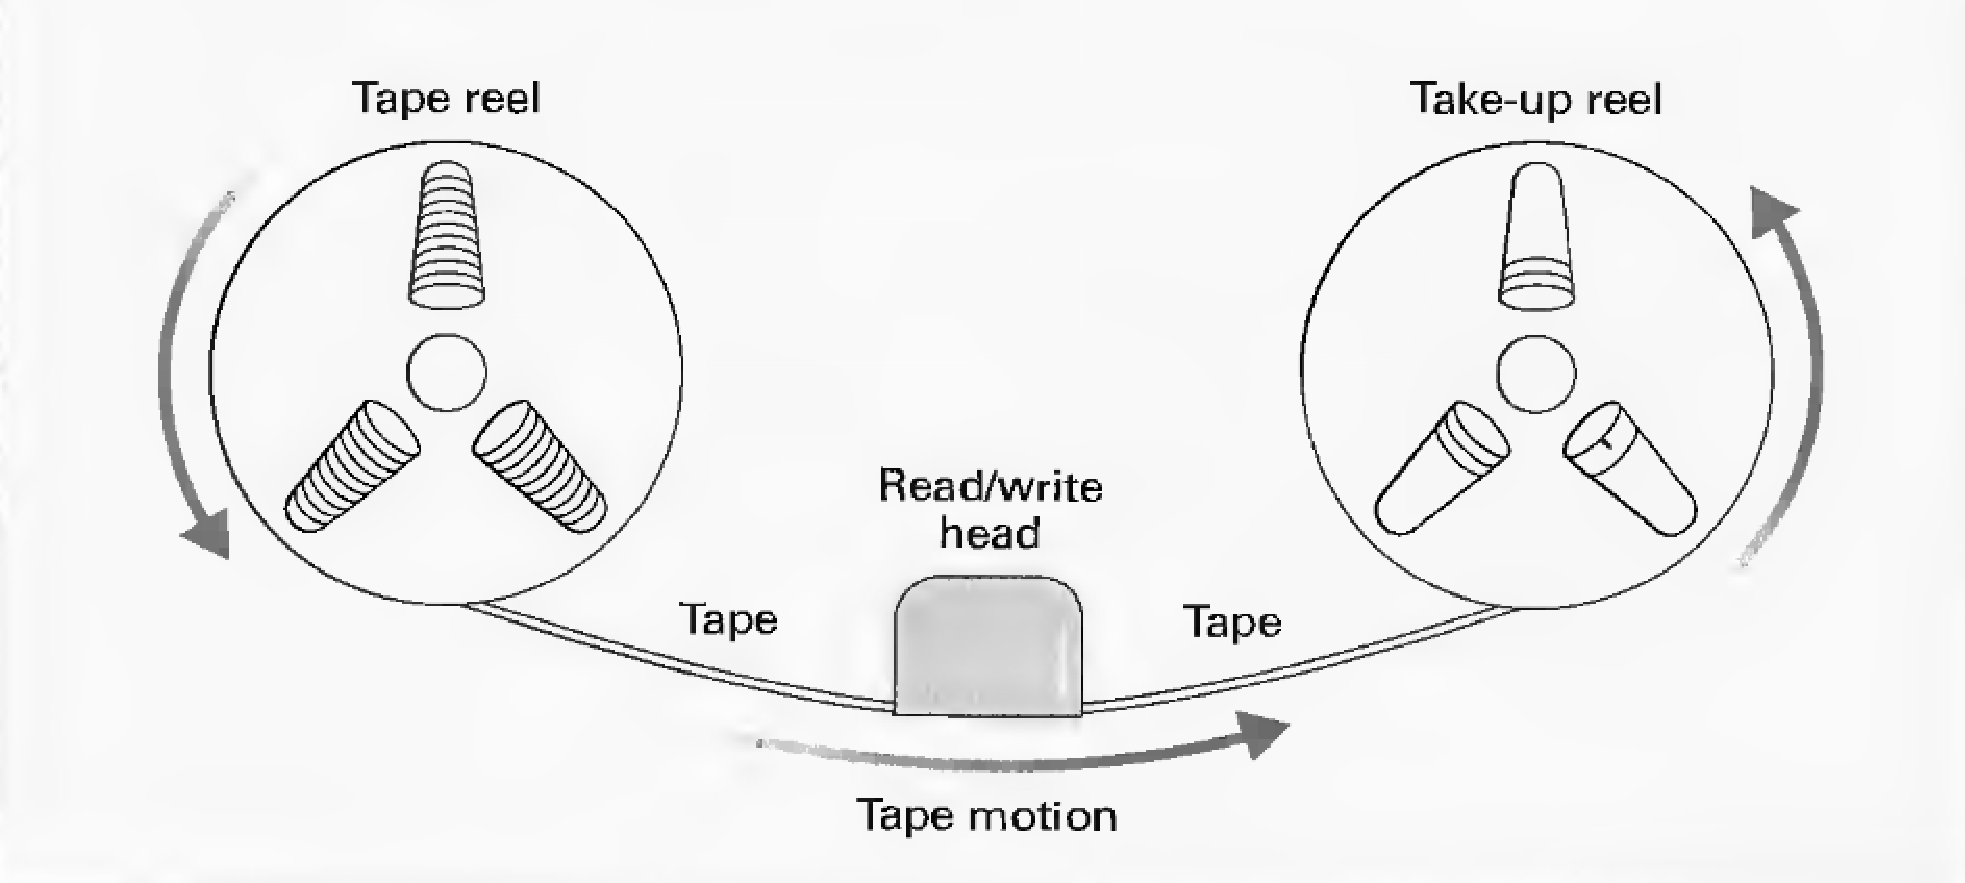
\includegraphics{ch2/Fig1-10.pdf}}
\caption{Cơ chế lưu trữ băng từ}
  \label{fig:fig1.10}
\end{figure}

\subsection*{Hệ thống quang}

Có một lớp thiết bị lưu trữ khối áp dụng kỹ thuật quang. Ví dụ đĩa \textbf{CD} (Compact
Disk). Các đĩa này có đường kính là $12$cm (xấp xỉ $5$ inches) và được phủ một lớp gương
với một lớp phủ bảo vệ. Thông tin được ghi trên đĩa bằng cách thay đổi bề mặt phản xạ. Vì
vậy, các thông tin này có thể được lưu trữ theo cách chùm tia laser được phóng không theo
quy luật trên bề mặt phản xạ của CD khi nó quay.

Công nghệ CD đã được ứng dụng trước đây cho việc thu âm dùng định dạng quen thuộc như
\textbf{CD-DA} (Compact disk-digital audio). Các đĩa CD sử dụng ngày nay về cơ bản có cùng
định dạng. Cụ thể, các thông tin trên các đĩa CD được lưu trữ trên một track đơn xoắn ốc
xung quanh CD giống cách ghi cũ, tuy nhiên điểm khác biệt là các track trên đĩa CD xoắn ốc
theo chiều từ trong ra~(Hình \ref{fig:fig1.11}). Track này được chia thành các đơn vị gọi
là sector, mỗi sector có định danh riêng của nó và có khả năng lưu giữ $2$KB dữ liệu,
tương đương với $\frac{1}{75}$ giây âm nhạc trong trường hợp ghi âm.
 
\begin{figure}[bth]
\centering
    \scalebox{0.3}{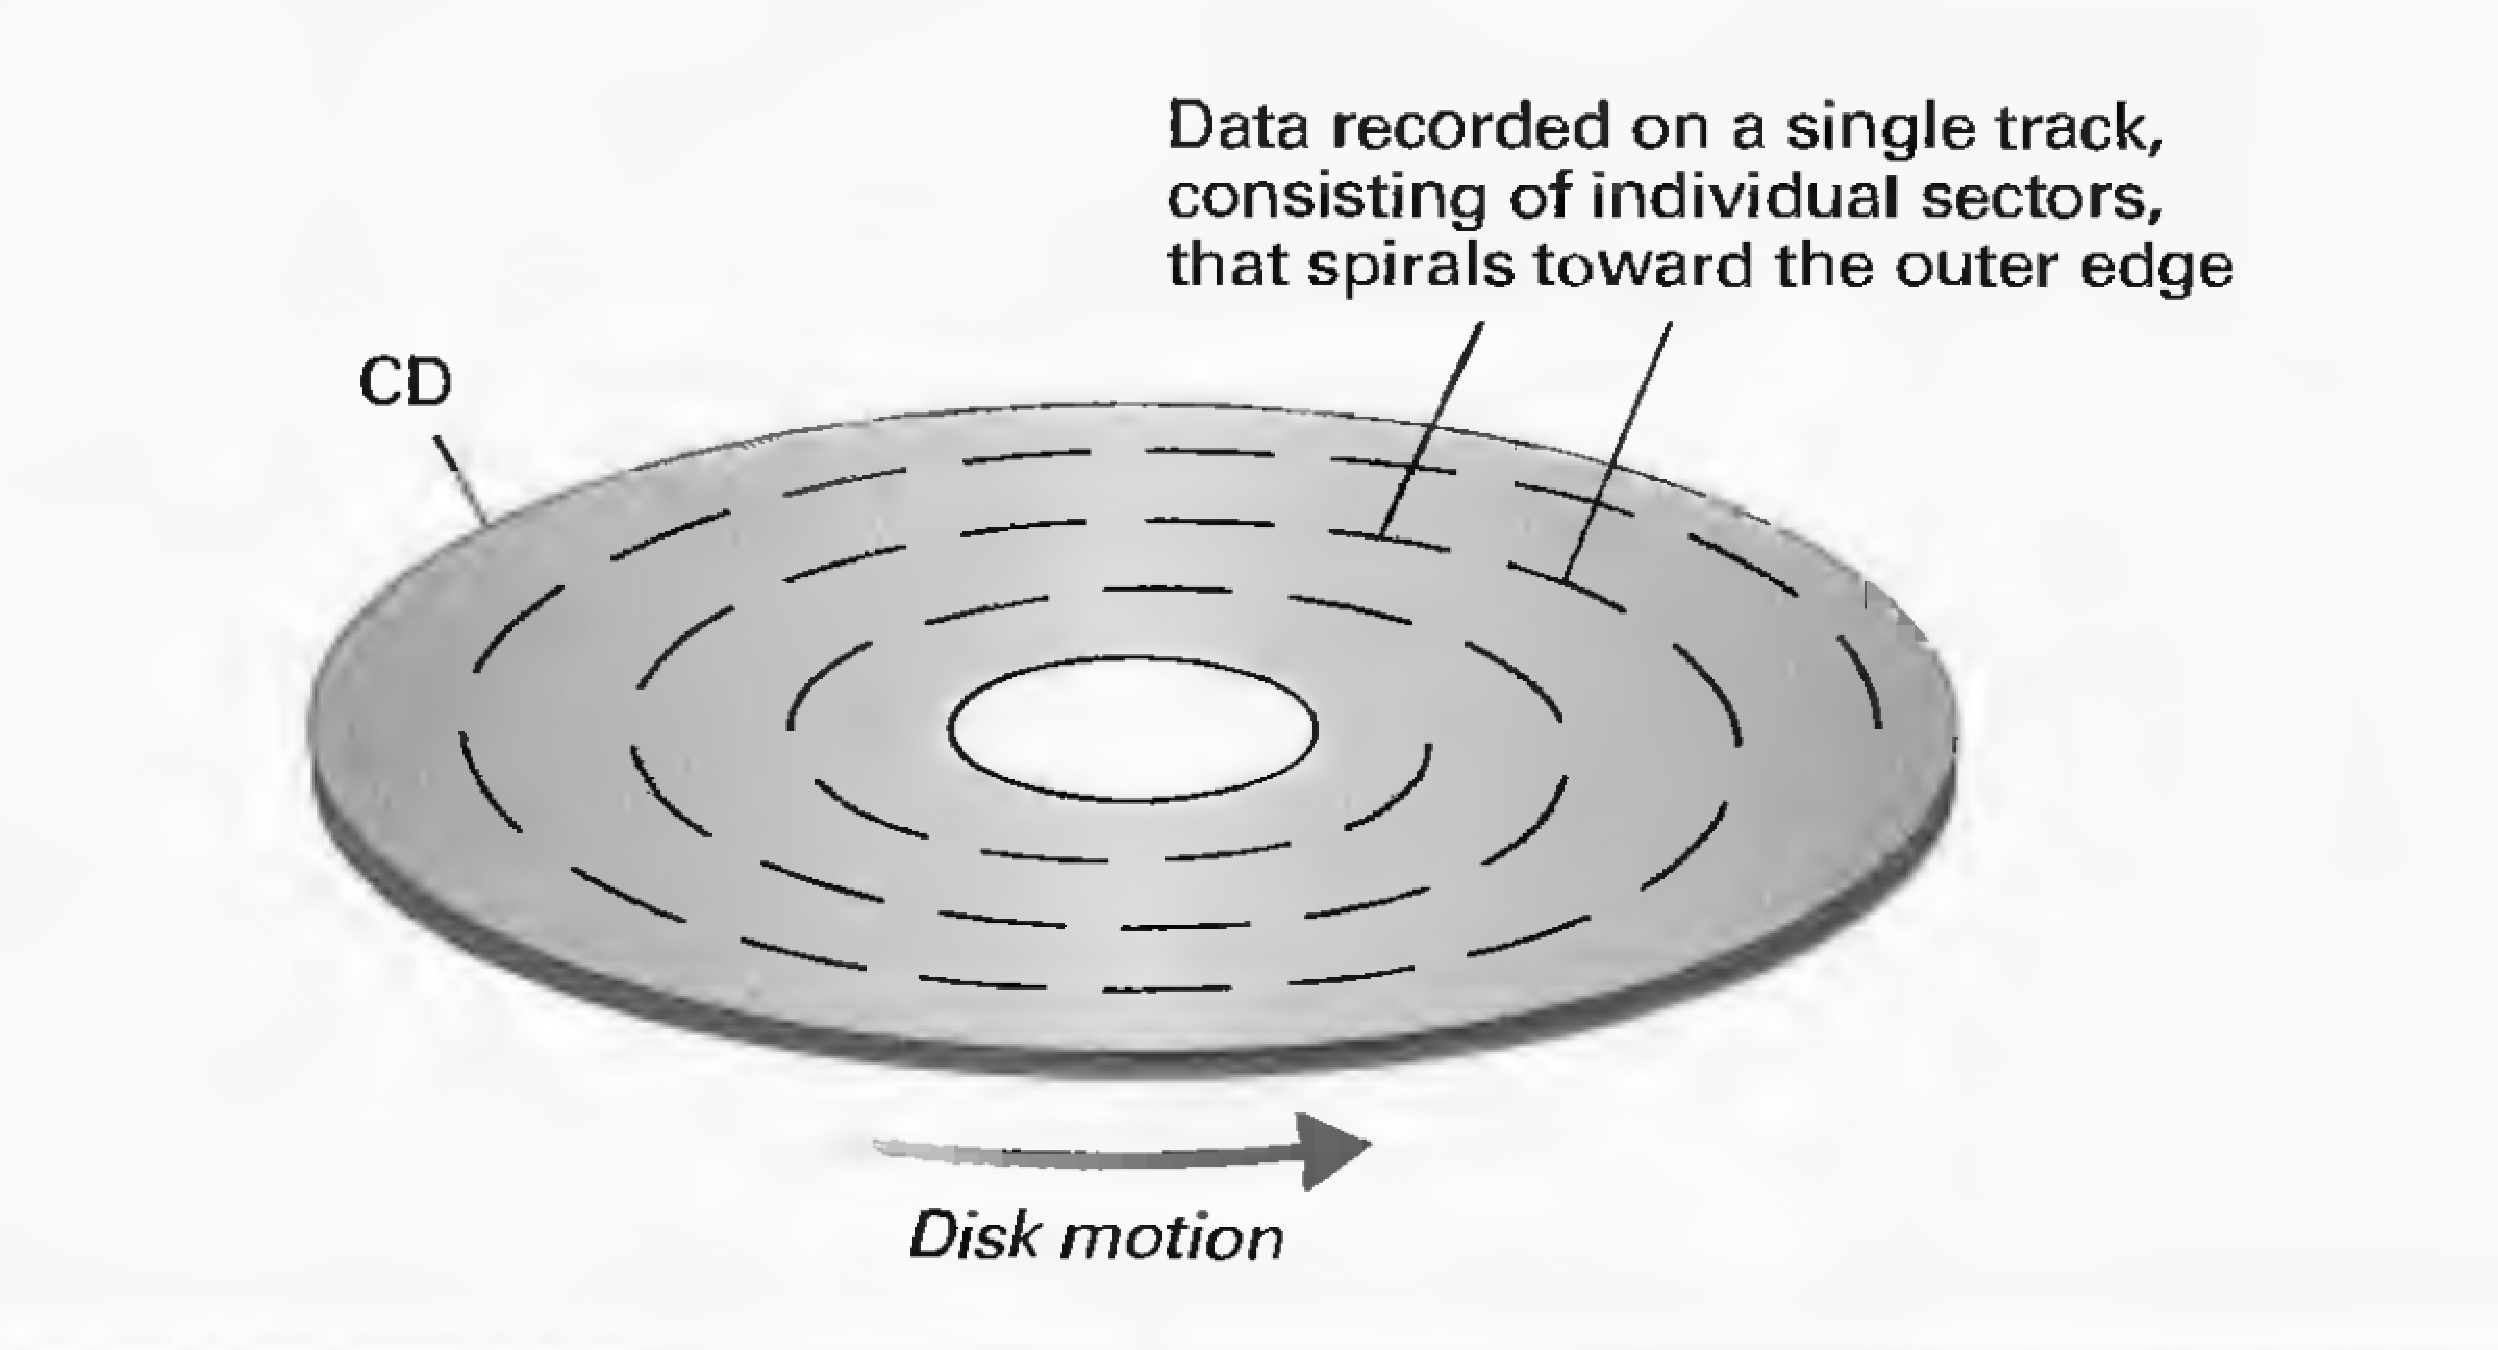
\includegraphics{ch2/Fig1-11.pdf}}
\caption{Định dạng lưu trữ của CD}
  \label{fig:fig1.11}
\end{figure}


% Chú ý rằng khoảng cách quanh track xoắn ốc là lớn dần từ trong ra
% ngoài. Để có thể có khả năng tốt nhất của một CD, các thông tin được
% lưu trữ theo mật đô phân phối tuyến tính chuẩn trên toàn bộ 

%[....]

Như một hệ quả của cách thiết kế, các hệ thống lưu trữ CD thực hiện tốt nhất với xâu dữ
liệu liên tục, dài, giống như khi sản xuất âm nhạc. Ngược lại, khi ứng dụng yêu cầu truy
cập ngẫu nhiên, cách tiếp cận dùng đĩa từ (gồm các track đồng tâm được chia thành các
sector có thể truy cập riêng biệt) làm tốt hơn cách tiếp cận xoắn ốc được dùng trong CDs.

Các đĩa CD truyền thống có khả năng lưu trữ $600$ đến $700$MB. Tuy nhiên, những đĩa
\textbf{DVD (Digital Versatile Disk)}, được xây dựng từ nhiều mối phức tạp, các tầng nửa
trong suốt phục vụ như bề mặt phân biệt khi được nhìn bởi một tia laser hội tụ một cách
chính xác, cho phép khả năng lưu trữ lên tới vài GB. Kiểu đĩa như thế này có khả năng lưu
trữ trình diễn đa phương tiện dài, bao gồm cả hình ảnh chuyển động.

\subsection*{Thiết bị Flash}

Một tính chất chung của thiết bị lưu trữ khối dựa trên công nghệ từ hoặc quang là chuyển
động vật lý như các đĩa xoay, di chuyển đầu đọc, và bắn chùm tia laser, được yêu cầu để
lưu trữ và lấy dữ liệu. Điều này có nghĩa rằng việc lưu trữ dữ liệu và tìm kiếm là chậm so
với mạch điện tử. Công nghệ \textbf{bộ nhớ flash} có khả năng giúp giảm bớt hạn chế
này. Trong hệ thống nhớ flash, các bít được lưu trữ bằng cách gửi tín hiệu điện trực tiếp
tới môi trường lưu trữ ở đó các electron được giữ trong một khoang nhỏ chứa silicon
dioxide, bởi vậy nó biến đổi các đặc trưng của mạch điện. Bởi vì các khoang chứa này có
khả năng giữ các electron trong nhiều năm, nên công nghệ này có thể phù hợp cho việc lưu
trữ dữ liệu off-line.

Mặc dù dữ liệu được lưu trữ trong hệ thống bộ nhớ flash có thể được truy cập theo đơn vị
kích thước nhỏ tính theo byte giống như trong ứng dụng RAM, nhưng hạn chế của công nghệ
hiện nay khiến cho dữ liệu phải được lưu trữ xoá theo khối lớn. Hơn nữa lặp lại việc xoá
sẽ gây thiệt hại cho khoang chứa silicon dioxide. Hạn chế này làm cho công nghệ bộ nhớ
flash hiện tại không thích hợp cho các ứng dụng bộ nhớ chính, nơi yêu cầu nội dung phải
thay đổi nhiều lần trong một giây. Tuy nhiên, đối với các ứng dụng mà tính thay đổi có thể
được điều chỉnh ở mức độ hợp lý như camera số, điện thoại di động, máy PDA cầm tay, thì bộ
nhớ flash lại trở thành thiết bị lưu trữ khối được lựa chọn. Thật vậy, bởi vì bộ nhớ flash
không nhạy cảm với các va chạm về mặt vật lý (ngược lại với hệ thống từ và quang) nên tiềm
năng của nó với các ứng dụng di động là rất hấp dẫn.

Các thiết bị flash được gọi là \textbf{flash drives}, với khả năng lên tới vài GB, là sẵn
có cho các ứng dụng lưu trữ khối tổng quát. Các đơn vị này được nén trong miếng nhựa nhỏ
có độ dài xấp xỉ ba inche cùng với nắp bảo vệ đơn vị kết nối điện khi thiết bị
off-line. Khả năng cao của các đơn vị di động này cũng như sự kiện rằng chúng dễ kết nối
và ngắt kết nối từ máy tính làm cho chúng trở thành lý tưởng cho việc lưu trữ dữ liệu
off-line. Tuy nhiên, tính dễ tổn thương của khoang lưu trữ làm cho chúng không tin cậy như
đĩa quang cho việc lưu trữ thực sự lâu dài.

\subsection*{Lưu trữ và tìm kiếm file}

Thông tin được lưu trữ trong hệ thống lưu trữ khối về mặt thiết kế được nhóm lại thành các
đơn vị lớn gọi là \textbf{file}. Một file điển hình có thể là một tài liệu văn bản được
hoàn thành, một tấm ảnh, một chương trình, một đĩa nhạc, hoặc một tập dữ liệu về nhân viên
trong công ty. Ta đã thấy rằng thiết bị lưu trữ khối làm cho các file được lưu trữ ít
hơn. Ví dụ, một file được lưu trữ trên một đĩa từ phải được xử lý theo sector, mà mỗi
sector có kích thước xác định trước. Một khối dữ liệu phù hợp với đặc trưng của thiết bị
lưu trữ được gọi là \textbf{bản ghi vật lý}. Bởi vậy, một file lớn được lưu trữ trong
thiết bị lưu trữ khối nói chung sẽ bao gồm nhiều bản ghi vật lý.

Ngược lại với cách chia theo các bản ghi vật lý này, một file thường phân chia tự nhiên
theo thông tin được biểu diễn. Ví dụ, một file chứa thông tin về nhân viên trong một công
ty có thể bao gồm nhiều đơn vị, mỗi đơn vị chứa thông tin về một nhân viên. Hoặc một file
chứa tài liệu văn bản có thể bao gồm nhiều đoạn hoặc trang văn bản. Các khối dữ liệu xuất
hiện tự nhiên như thế này được gọi là \textbf{các bản ghi logic}.


Các bản ghi logic thường bao gồm các đơn vị nhỏ hơn gọi là các \textbf{trường}. Ví dụ, một
bản ghi logic chứa thông tin về nhân viên có thể bao gồm trường tên, địa chỉ, số chứng
minh của nhân viên,... Đôi khi mỗi bản ghi logic trong một file xác định một cách duy nhất
bởi một trường đặc biệt bên trong bản ghi (có thể là số chứng minh thư của nhân viên, một
số, hoặc chỉ mục trong bảng liệt kê). Trường xác định như thế này được gọi là
\textbf{trường khoá}. Giá trị giữa trong trường khoá được gọi là \textbf{khoá}.
\begin{figure}
\centering
    \scalebox{0.3}{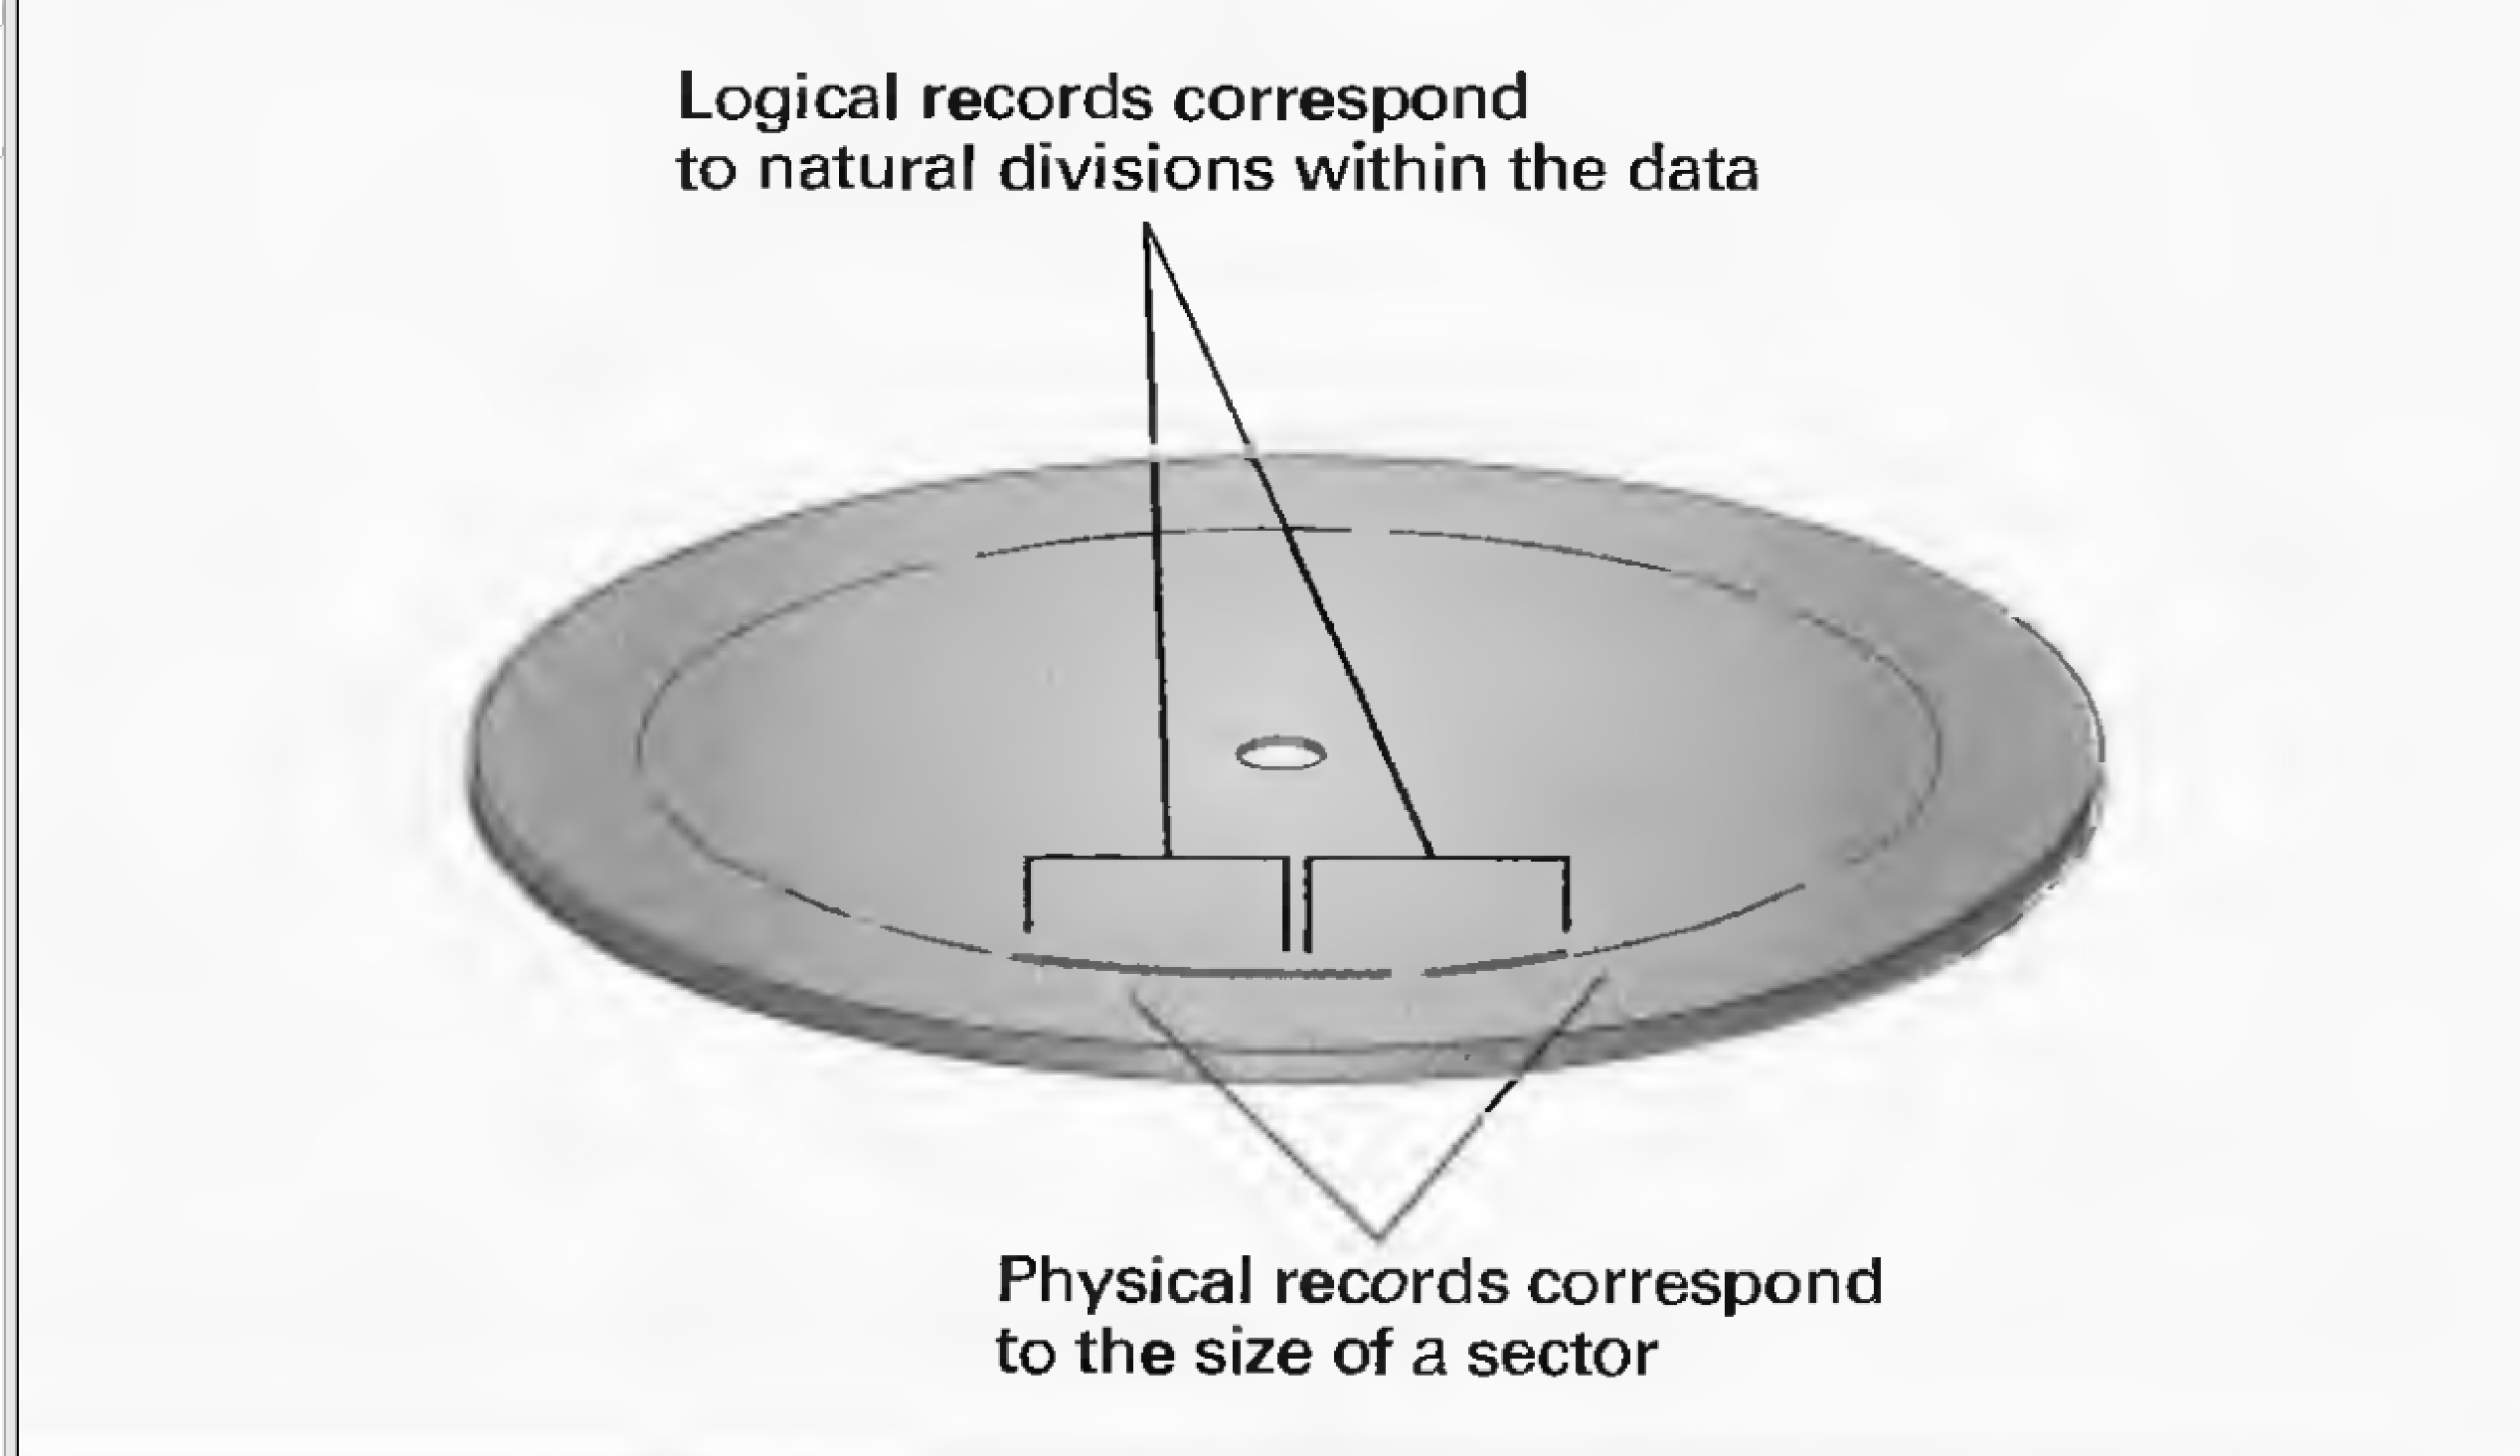
\includegraphics{ch2/Fig1-12.pdf}}
\caption{Bản ghi logic và bản ghi vật lý trên một đĩa}
  \label{fig:fig1.12}
\end{figure}

Các kích thước của bản ghi logic hiếm khi được so sánh với kích thước bản ghi vật lý của
của thiết bị lưu trữ khối. Nói cách khác, người ta có thể tìm thấy một vài bản ghi logic
nằm bên trong một bản ghi vật lý hoặc có thể là một bản ghi logic tách thành hai hoặc
nhiều bản ghi vật lý (Hình \ref{fig:fig1.12}). Kết quả là việc tìm kiếm dữ liệu từ thiết
bị lưu trữ khối phải kèm thêm với việc phục hồi những lộn xộn này. Một giải pháp chung cho
vấn đề này là đặt bên ngoài bộ nhớ chính khoảng đủ lớn lưu giữa một vài bản ghi vật lý và
để sử dụng không gian bộ nhớ này như một vùng nhóm lại. Có nghĩa rằng, các khối dữ liệu
thích hợp với bản ghi vật lý có thể được truyền giữa bộ nhớ chính và thiết bị lưu trữ
khối, trong khi dữ liệu nằm trong bộ nhớ chính có thể được tham khảo như bản ghi logic.


Một vùng bộ nhớ dùng theo cách này được gọi là \textbf{vùng đệm} (buffer). Nói chung, một
vùng đệm là một vùng nhớ được dùng để lưu trữ dữ liệu trung gian trong quá trình truyền dữ
liệu từ thiết bị này tới thiết bị khác. Ví dụ, các máy in hiện đại có chứa mạch nhớ riêng,
phần lớn của mạch này được dùng như vùng đệm để lưu trữ các phần của tài liệu còn chưa
được in mà máy in nhận được.
  
\subsection*{Câu hỏi \& Bài tập}

\begin{enumerate}
\item Hệ thống đĩa cứng có ưu điểm gì so với đĩa mềm khi các đĩa của nó quay nhanh hơn các
  đĩa của đĩa mềm?

\item Khi ghi dữ liệu trên hệ thống nhiều đĩa, ta nên hoàn thành hết bề mặt đĩa trước khi
  bắt đầu bề mặt khác, hay ta đầu tiên nên hoàn thành hết cylinder trước khi bắt đầu sang
  cylinder khác?

\item Trong một hệ thống đặt chỗ, dữ liệu thường phải cập nhật liên tục. Tại sao dữ liệu
  này nên được lưu trữ trên đĩa từ thay vì CD hay DVD?

\item Khi sửa một tài liệu với trình xử lý văn bản, đôi khi việc thêm đoạn văn bản không
  làm tăng kích thước bên ngoài của file trong lưu trữ khối. Nhưng có lúc chỉ thêm một kí
  tự cũng có thể làm tăng kích thước của file tới vài nghìn byte. Bạn hãy giải thích xem
  tại sao?

\item Nêu một vài ưu điểm của thiết bị flash so với hệ thống lưu trữ khác được giới thiệu
  trong phần này?


\item Vùng đệm là gì?
  
\end{enumerate}


  

%%% Local Variables: 
%%% mode: latex
%%% TeX-master: "../tindaicuong"
%%% End: 


\section{Biểu diễn thông tin}

Ta đã xem xét các kỹ thuật để lưu trữ các bít, bây giờ ta sẽ xem xét cách mã hoá thông tin
như dãy bít. Ta sẽ quan tâm đến các phương pháp phổ biến để mã hoá văn bản, dữ liệu số,
hình ảnh, âm thanh. [....]

\subsection*{Biểu diễn văn bản}
Thông tin của văn bản thường được biểu diễn bởi mã của các ký hiệu trong nó (như các chữ
cái trong một bảng chữ, các dấu chấm, phảy,...). Từ đó, văn bản được biểu diễn như một xâu
bít dài trong đó dãy bít liên tiếp biểu diễn các ký hiệu liên tiếp trong văn bản gốc.

Trong những năm~$1940$ và~$1950$, nhiều kiểu mã như vậy đã được thiết kế và được sử dụng
trong liên lạc giữa các thành phần khác nhau của thiết bị, điều này cũng dẫn đến phức tạp
trong truyền thông. Để làm giảm những phức tạp này, \textbf{Hội Chuẩn Quốc Gia Hoa Kỳ
  (ANSI)} đã chọn Mã chuẩn của Mỹ để trao đổi thông tin (\textbf{American Standard Code
  for Information Interchange (ASCII)}). Mã này dùng các xâu bảy bít để biểu diễn các chữ
cái hoa và chữ cái thường của bảng chữ Tiếng Anh, ký hiệu dấu, các số từ $0$ tới $9$, và
một số thông tin điều khiển như ký hiệu xuống dòng, ký hiệu trở về, và tab. Ngày nay, mã
ASCII được mở rộng sang thành dạng tám bít bằng cách thêm một $0$ vào bít trái nhất của
xâu bảy bít. Kỹ thuật này không chỉ cho ta một mã phù hợp với kích thước ô nhớ theo byte
mà còn cho ta thêm $128$ bít nữa (những mã bắt đầu bởi $1$) là những ký hiệu mở rộng thêm
từ bảng mã ASCII ban đầu. Không may, mỗi nhà sản xuất hướng sử dụng các ký hiệu được mở
rộng theo cách riêng của họ, nên dữ liệu mà các xâu bít này biểu diễn không dễ chuyển từ
các ứng dụng của nhà sản xuất này sang ứng dụng của nhà sản suất khác.

Một phần của ASCII theo định dạng xâu tám bít cho mỗi ký hiệu được chỉ ra bởi Phụ lục
\ref{}. Bằng cách tra phụ lục này, ta có thể giải mã xâu bít Hình~\ref{fig:fig1.13}
như thông điệp ``Hello.''.

\begin{figure}[bt]
\centering
\begin{tabular}{cccccc}
  $\underbrace{01001000}$ & $\underbrace{01100101}$
  & $\underbrace{01101100}$ & $\underbrace{01101100}$  
  & $\underbrace{01101111}$ & $\underbrace{00101110}$ \\
  \texttt{H}  & \texttt{e}  & \texttt{l} & \texttt{l} & \texttt{o}
  & \texttt{.}                                        \\
\end{tabular}
\caption{Thông điệp ``Hello.'' biểu diễn ở ASCII}
  \label{fig:fig1.13}
\end{figure}

Mặc dù bảng mã ASCII đã được thừa nhận rộng rãi trong nhiều năm, tuy nhiên do nhu cầu trình
bày tài liệu trong nhiều ngôn ngữ, những mã khác mở rộng hơn hiện nay lại trở nên phổ
biến. Một trong số đó là \textbf{Unicode}, đã được phát triển nhờ hợp tác của một vài nhà
sản xuất phần cứng hàng đầu và nhanh chóng nhận được sự ủng hộ của cộng đồng quốc tế. Mã
này dùng một xâu $16$ bít duy nhất để biểu biễn một ký hiệu. Vậy, Unicode bao gồm $65,536$
xâu bít khác nhau--đủ để biểu diễn các văn bản ở nhiều ngôn ngữ như Tiếng Trung, Tiếng
Nhật, và Tiếng Do Thái.

Chuẩn hoá cho một bộ mã đầy đủ Unicode được phát triển bởi \textbf{Tổ chức Quốc Tế về
  Chuẩn hoá} (International Organization for Standardization, viết tắt là
\textbf{ISO}). Mã này dùng các xâu độ dài $32$ bít, và có khả năng biểu diễn hàng tỉ ký
hiệu khác nhau.

Một file bao gồm một dãy ký hiệu dài được mã hoá dùng ASCII hoặc Unicode thường được gọi
là một \textbf{file văn bản}. Một ý quan trọng mà ta phải phân biệt, đó là giữa một file
văn bản đơn giản có thể thao tác bởi các chương trình công cụ được gọi là \textbf{trình
  soạn thảo} và các file phức tạp hơn được tạo bởi \textbf{bộ xử lý văn bản}. Cả hai đều
bao gồm các văn bản. Tuy nhiên, một file văn bản chỉ chứa các ký hiệu mã hoá của văn bản,
trong khi đó một file tạo bởi bộ xử lý văn bản chứa nhiều mã riêng biểu diễn các font, các
thông tin về cách gióng hàng,... Hơn nữa, bộ xử lý văn bản có thể sử dụng các mã riêng
thay vì chuẩn ASCII hoặc Unicode để biểu diễn văn bản.

\subsection*{Biểu diễn giá trị số}

Lưu trữ thông tin theo cách mã hoá các ký tự là không hiệu quả khi thông tin là các giá
trị số. Để thấy lý do tại sao, ta cùng xem xét vấn đề lưu trữ giá trị $25$. Nếu ta nhất
định lưu trữ nó như các ký hiệu ở dạng ASCII dùng mỗi byte cho mỗi ký hiệu, ta cần $16$
bít để lưu trữ. Hơn nữa, số lớn nhất ta có thể lưu trữ dùng $16$ bít là $99$. Tuy nhiên,
nếu dùng \textbf{ký hiệu nhị phân} thì với $16$ bít ta có thể lưu trữ mọi số nguyên từ $0$
tới $65,535$. Bởi vậy, ký hiệu nhị phân (hay các dạng khác của nó) được sử dụng rộng rãi
cho việc mã hoá dữ liệu số trên máy tính.

Ký hiệu nhị phân là một cách biểu diễn các giá trị số chỉ dùng các số $0$ và $1$ thay vì
các số $0, 1, 2 , 3, 4, 5, 6, 7, 8, $ và $9$ như trong chữ số truyền thống, hoặc cơ sở
$10$. ta sẽ nghiên cứu hệ thống số đầy đủ trong Mục \ref{}. Bây giờ, ta sẽ chỉ cần một vài
kiến thức cơ sở để hiểu hệ thống này. Với mục đích này, ta sẽ xem xét đồng hồ đo số km
trong các ôtô kiểu cũ [.....]

Do tính hiệu quả này, các thông tin dạng số thường được lưu trữ bởi một dạng ký hiệu nhị
phân thay vì dạng ký hiệu được mã hoá. Ta nói ``một dạng ký hiệu nhị phân'' bởi vì hệ
thống nhị phân được mô tả trực tiếp chỉ là cơ sở cho một vài kỹ thuật lưu trữ số được sử
dụng bên trong máy. Một vài dạng khác của hệ thống nhị phân sẽ được thảo luận sau này. Bây
giờ, ta thuần tuý chỉ để ý rằng hệ thống được gọi là ký hiệu \textbf{bù hai} (xem Phần
\ref{}) là cách chung để lưu trữ các số bởi vì nó cho ta phương pháp thích hợp để biểu
diễn số ấm cũng như số nguyên dương. Để biểu diễn phân số như $4\frac{1}{2}$ hoặc
$\frac{3}{4}$, được gọi là ký hiệu \textbf{dấu chấm động} (xem Mục \ref{}).

\subsection*{Biểu diễn hình ảnh}

Các ứng dụng máy tính ngày nay bao gồm nhiều hơn là chỉ có văn bản và giá trị số. Chúng
còn bao gồm cả hình ảnh, âm thanh, và video. Kỹ thuật phổ biến để biểu diễn ảnh bao gồm
hai loại: \textbf{các kỹ thuật bitmap} và \textbf{các kỹ thuật vectors}. Với kỹ thuật bit
map, một ảnh được biểu diễn như một tập các điểm, mỗi điểm gọi là một \textbf{pixel}, viết
tắt của từ ``picture element.'' (phần tử ảnh). Một ảnh đen trắng được mã hoá như một xâu
bít dài biểu diễn các dòng pixel trong ảnh, trong đó mỗi bít hoặc là bằng $1$ hoặc
bằng~$0$ phụ thuộc khi nào pixel tương ứng là đen hay trắng. Kỹ thuật này được sử dụng
trong hầu hết các máy sao chép (facsimile).

Thuật ngữ \textit{bit map} bắt nguồn từ sự kiện rằng các bít biểu diễn một ảnh theo định
dạng một-bít-cho-một-pixel [...]. Ngày nay thuật ngữ đã được tổng quát hoá để bao gồm mọi
hệ thống trong đó các ảnh được mã hoá theo cách pixel-cạnh-pixel. Ví dụ, trong trường hợp
ảnh đen trắng, mỗi pixel được biểu diễn bởi một tập các bít (thường là tám), cho phép bóng
xám được biểu diễn.

Cách tiếp cận bip map được mở rộng cho ảnh màu, trong đó mỗi điểm ảnh (pixel) được biểu
diễn bởi một tổ hợp các bít chỉ ra có mặt của pixel. Hai cách tiếp cận này là chung. Trong
đó, cách ta sẽ gọi là mã hoá RGB, mỗi điểm ảnh được biểu diễn bởi thành phần màu-- đỏ
(red), xanh lá cây (green) và xanh lam (blue)--tương ứng với ba màu của ánh sáng. Thông
thường ta dùng một byte để biểu diễn cường độ của mỗi thành phần màu. Bởi vậy, mỗi điểm
ảnh cần ba byte để lưu trữ.

Một lựa chọn phổ biến khác để mã hoá RGB là sử dụng thành phần ``độ sáng'' kết hợp với hai
thành phần màu. Ở đây, thành phần ``độ sáng'' được gọi là độ chiếu sáng của điểm ảnh, về
cơ bản nó là tổng của ba thành phần đỏ, xanh lá cây và xanh lam. (Trên thực tế, nó chính
là tổng số ánh sáng trắng trong điểm ảnh, nhưng ở đây ta sẽ không cần quan tâm chi tiết.)
Hai thành phần còn lại được gọi là độ màu xanh lam và độ màu đỏ. Độ màu xanh lam (tương
ứng, độ màu đỏ) được xác định bằng cách tính chênh lệch giữa độ chiếu sáng của điểm ảnh và
tổng số ánh sáng xanh lam (tương ứng tổng số ánh sáng đỏ) trong điểm ảnh. Kết hợp cả ba
thành phần này lại ta được thông tin xác định điểm ảnh.

Tính phổ biến của mã hoá ảnh dùng độ sáng và các thành phần màu bắt nguồn từ lĩnh vực
truyền hình màu bởi vì cách tiếp cận này cho phép tương thích giữa việc mã hoá các ảnh màu
và các tín hiệu nhận được của các tivi đen trắng đời cũ. Thực ra, các ảnh xám có thể được
xem như ảnh màu khi giới hạn chỉ dùng thành phần độ sáng.

Một điểm bất lợi của kỹ thuật bitmap là ảnh không thể thay đổi kích thước một cách tuỳ
ý. Về cơ bản, chỉ có cách phóng to ảnh là tăng độ lớn của điểm ảnh, nhưng nó sẽ làm vỡ
ảnh. (Đây là kỹ thuật dùng trong các camera số gọi là ``digital zoom'', ngược lại với
``optical zoom'' là điều chỉnh thấu kính của cameras.) Kỹ thuật vector cho phép khắc phục
vấn đề này. Với cách tiếp cận này, một ảnh được biểu diễn như một tập các đường thẳng và
đường cong. Kiểu mô tả này bỏ qua chi tiết xem làm thế nào các đường thẳng và đường cong
được vẽ ra thiết bị tạo ảnh mà thay vào đó nó nhấn mạnh đến cách tạo ra một mẫu điểm ảnh
đặc biệt.

Nhiều font trong các hệ thống xử lý văn bản ngày nay được mã hoá dùng kỹ thuật vector. Kỹ
thuật này cho phép làm thay đổi kích thước của ký tự trong văn bản một cách mềm dẻo. Các
font này được gọi là \textbf{scalable fonts}. Ví dụ, TrueType (được phát triển bởi
Microsoft và Apple Computer) là một hệ thống mô tả cách các ký hiệu trong văn bản được
vẽ. Tương tự, PostScript (được phát triển bởi Adobe System) cho phép mô tả các ký tự cũng
như các dữ liệu ảnh tổng quát hơn. Các kỹ thuật biểu diễn vector cũng phổ biến trong các
hệ thống \textbf{thiết kế với trợ giúp của máy tính} (Computer-aided design) trong đó việc
vẽ các đối tượng ba chiều được hiện và được thao tác trên màn hình máy tính.

\subsection*{Biểu diễn âm thanh}

Phương pháp chung nhất để mã hoá thông tin audio để lưu trữ và xử lý trong máy tính là lấy
mẫu biên độ của sóng âm theo từng khoảng và ghi lại như dãy giá trị. Ví dụ, dãy $0$,
$1.5$, $2.0$, $3.0$, $4.0$, $3.0$, $0$ là dãy sóng âm theo biên độ, nói một cách ngắn gọn,
sóng này tăng dần rồi quay lại $0$ (Hình \ref{fig:fig1.14}). Kỹ thuật này sử dụng một tỷ lệ lấy mẫu
là $8000$ mẫu mỗi giây, đã được dùng trong nhiều năm để truyền thông điện thoại khoảng
cách xa. Giọng nói được mã hoá bằng giá trị số biểu diễn biên độ của giọng $8000$ lần
trong một giây. Các giá trị này được truyền đến nơi nhận, tại đây âm của giọng được tái
tạo lại.


Dù tỷ lệ $8000$ mẫu trên giây có vẻ khá nhanh, nhưng nó vẫn không đủ để thu âm với độ
trung thực cao. Để đạt được chất lượng âm thanh cao của đĩa CD nhạc, một tỷ lệ mẫu
$44,100$ mẫu trên giây được dùng. Dữ liệu đạt được từ mỗi mẫu được biểu diễn bởi $16$ bít
($32$ bít cho thu âm stereo). Vậy nên ta cần hơn một triệu bít cho mỗi giây của âm nhạc
thu ở dạng stereo.

\begin{figure}[tbh]
\centering
    \scalebox{0.65}{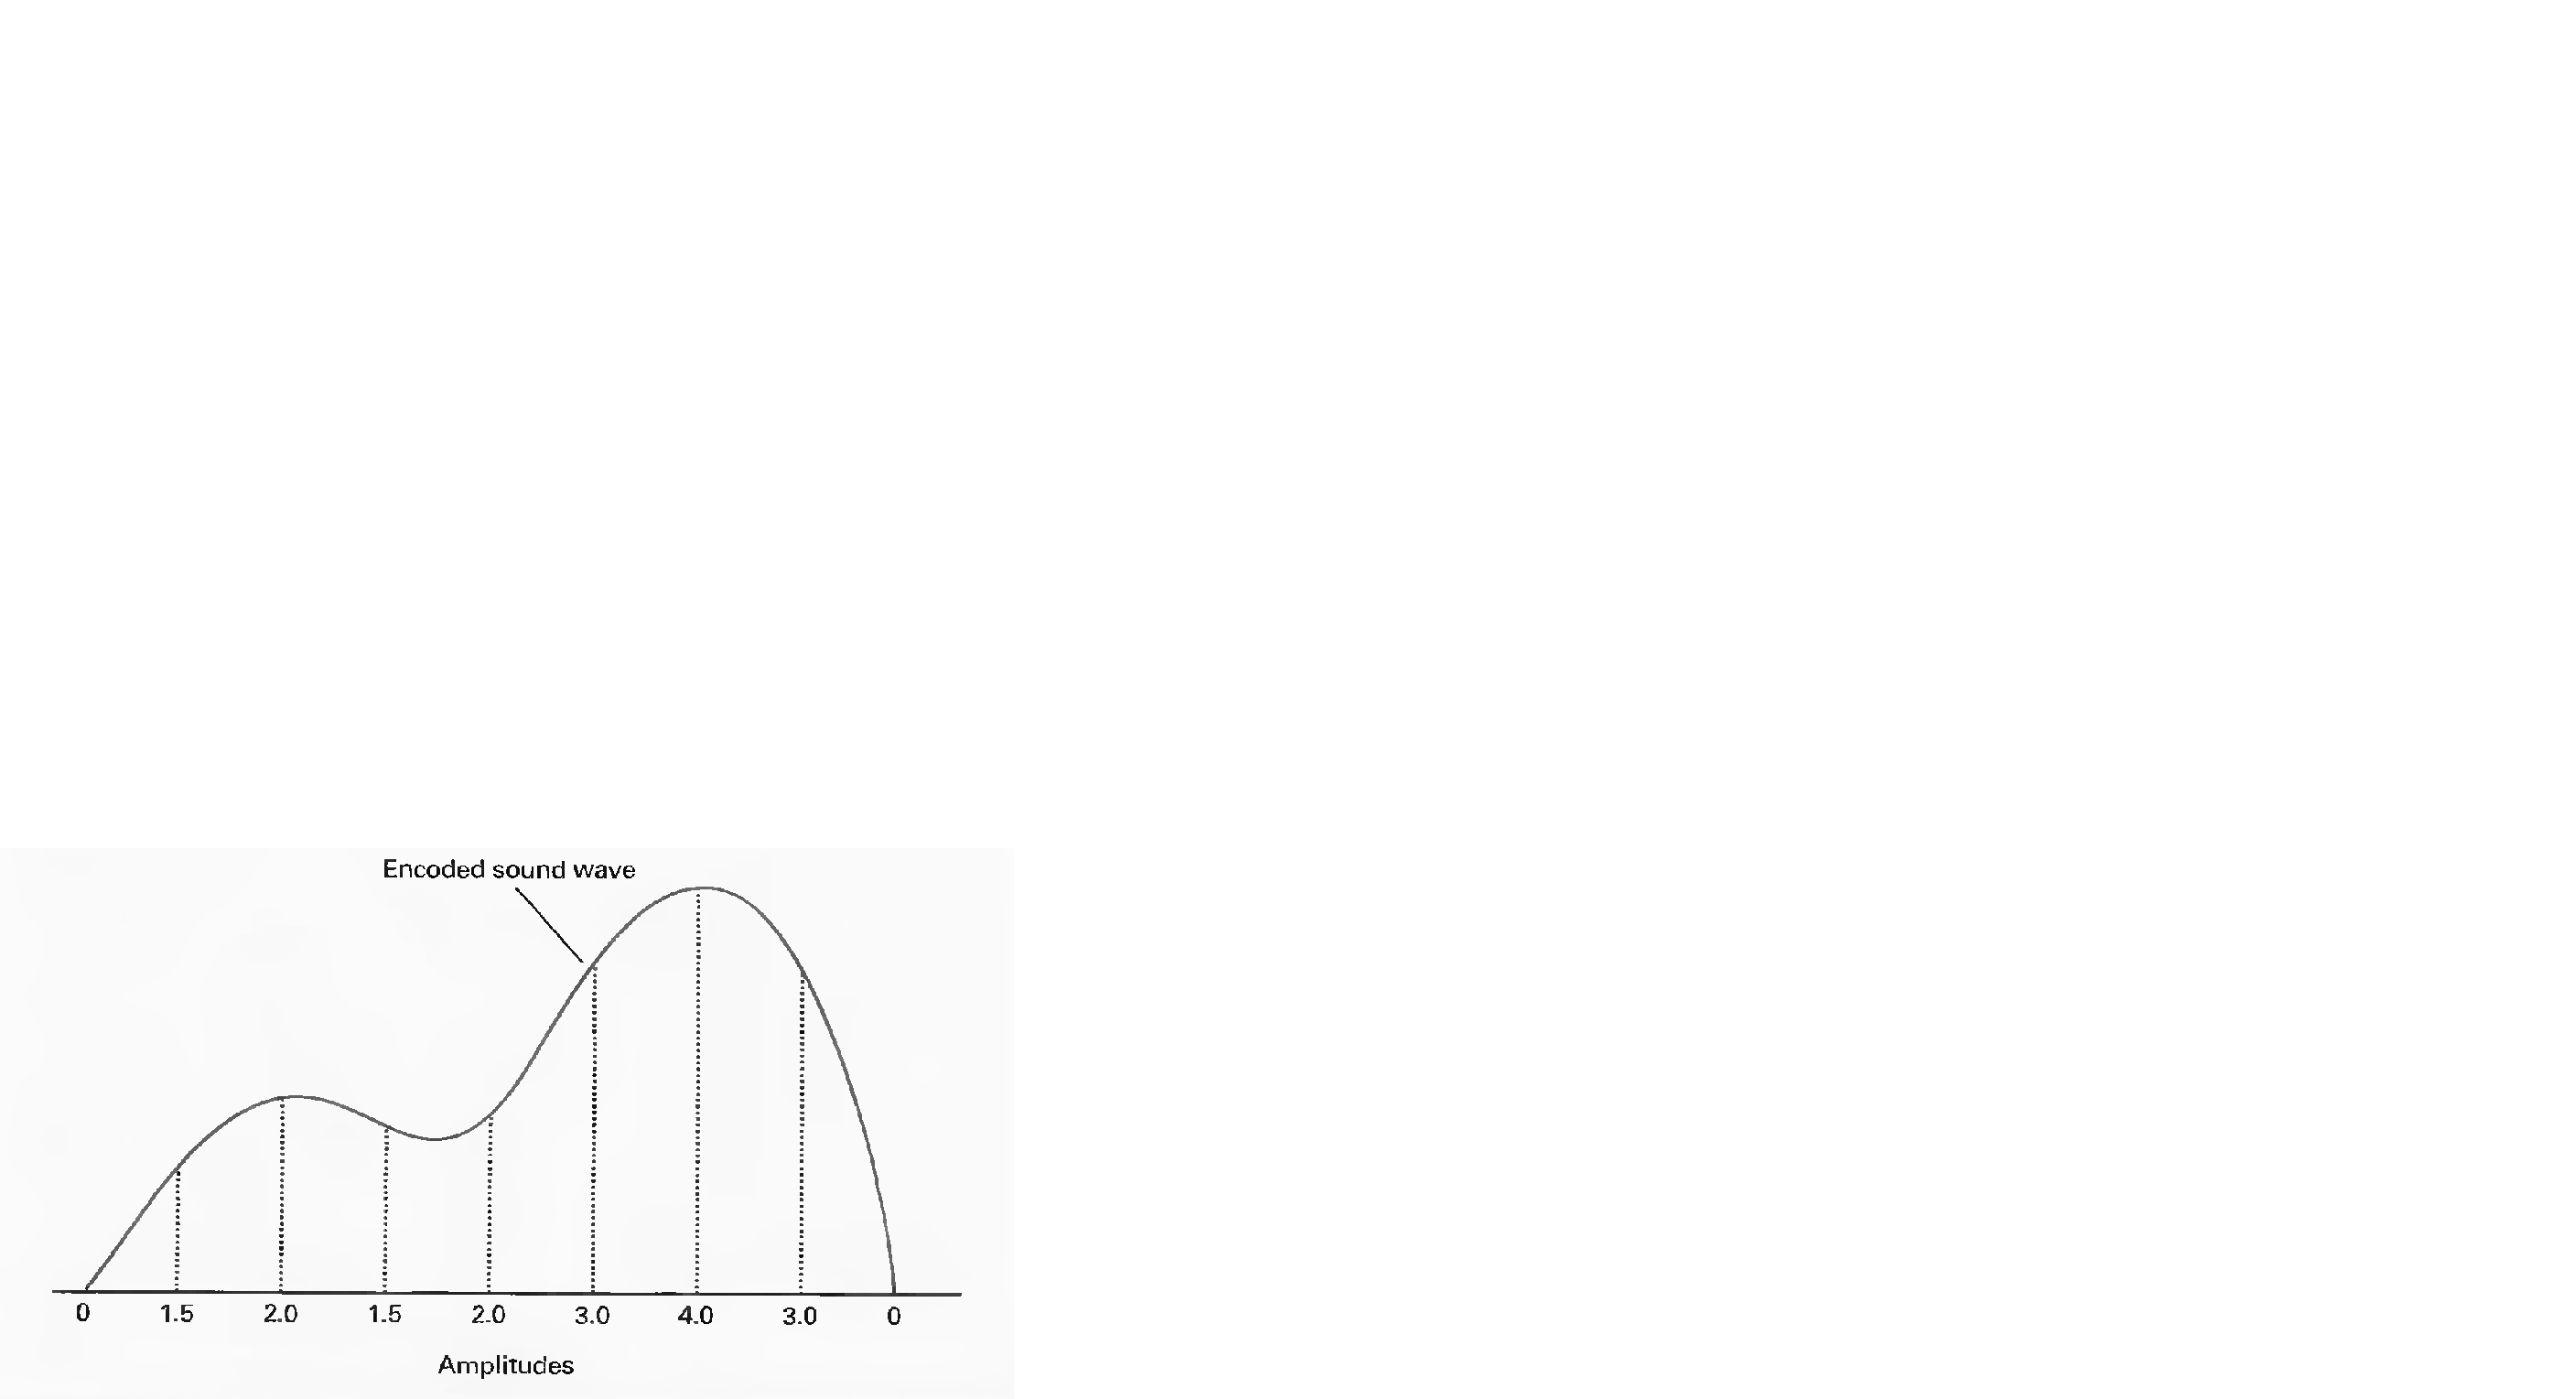
\includegraphics{ch2/Fig114.pdf}}
    \caption{Sóng âm được biểu diễn bởi dãy $0$, $1.5$, $2.0$, $3.0$, $4.0$, $3.0$, $0$}
  \label{fig:fig1.14}
\end{figure}


Một hệ thống mã hoá khác là Musical Instrumental Digital Interface (MIDI) được sử dụng
rộng rãi được sử dụng trong các bộ tổng hợp được tìm thấy trong các bàn phím điện tử,
trong âm thanh của các trò chơi video, và trong âm thanh hiệu ứng kèm các các trang
web. Bằng cách mã hoá các chỉ dẫn để tạo ra âm cho một thiết bị tổng hợp thay vì phải mã
hoá bản thân âm thanh, MIDI tránh được các yêu cầu lưu trữ lớn của kỹ thuật lấy mẫu. Chính
xác hơn, MIDI mã hoá các nốt nhạc của các nhạc cụ theo thời gian, ví dụ clarinet chơi nốt
Rê trong hai giây có thể mã hoá bằng ba byte thay vì mất hơn hai triệu bít bằng cách lấy
mẫu với tỷ lệ $44,100$ mẫu trên giây.

Nói tóm lại, ta có thể nghĩ MIDI như cách mã hoá các bản nhạc đọc bởi người biểu diễn thay
vì chính bản thân việc trình diễn, và việc chơi một file MIDI có thể nghe rất khác trên
các thiết bị tổng hợp khác nhau.

\subsection*{Câu hỏi \& Bài tập}

\begin{enumerate}
\item Đây là một thông điệp được mã hoá ở dạng ASCII dùng tám bít cho mỗi ký hiệu. Thông
  điệp này ý nghĩa là gì? (Xem Phụ lục \ref{})

\begin{tabular}{cccccc}
  01000011 &01101111 &01101101 &01110000 &01110101 &01110100  \\
  01100101 &01110010 &00100000 &01010011 &01100011 &01101001  \\
  01100101 &01101110 &01100011 &01100101 & &
\end{tabular}


\item Hãy chỉ ra mối quan hệ giữa mã của ký tự hoa và ký tự thường của
  cùng một ký tự theo bảng mã ASCII.

\item Mã hoá các câu sau theo bảng mã ASCII.
  \begin{enumerate}
  \item Where are you?

  \item "How?" Cheryl asked.

  \item 2 + 3 = 5.
  \end{enumerate}

\item Hãy mô tả một thiết bị trong cuộc sống hàng ngày có thể ở một trong hai trạng thái,
  ví dụ như lá cờ cắm trên cột cờ có thể ở trạng thái được treo hay không treo. Gán ký
  hiệu $1$ tới một trong hai trạng thái này và $0$ cho trạng thái còn lại, và chỉ ra cách
  biểu diễn ASCII cho ký tự $b$ khi lưu trữ dùng kiểu bít này.

\item Chuyển mỗi biểu diễn nhị phân sau đây sang cơ số mười:

  \begin{inparaenum}
  \item $0101 $ \hspace{2cm}
  \item $1001 $ \hspace{2cm}
  \item $1011 $

  \item $0110 $ \hspace{2cm}
  \item $10000$ \hspace{2cm}
  \item $10010$
  \end{inparaenum}

\item Chuyển mỗi biểu diễn thập phân sau đây sang nhị phân:

  \begin{inparaenum}
  \item $6$ \hspace{2cm} 
  \item $13$ \hspace{2cm}
  \item $11$ \hspace{2cm}


  \item $18$ \hspace{2cm}
  \item $27$ \hspace{2cm}
  \item $4$
  \end{inparaenum}

\item Nếu mỗi chữ số được mã hoá bởi một byte theo ASCII thì giá trị số lớn nhất có thể
  được biểu diễn dùng ba bytes là bao nhiêu? cũng vẫn ba byte đó nếu ta dùng ký hiệu nhị
  phân thì giá trị số lớn nhất là bao nhiêu?

\item Một lựa chọn khác so với ký hiệu hexa để biểu diễn dãy bít là \textbf{ký hiệu thập
    phân ngăn cách bởi dấu chấm} trong đó mỗi byte biểu diễn bởi giá trị ở cơ sở $10$
  tương đương. byte biểu diễn một số ngăn cách bởi các dấu chấm. Ví dụ, $12.5$ biểu diễn
  xâu $0000110000000101$ (byte $00001100$ biểu diễn số $12$, và $00000101$ biểu diễn số
  $5$), và xâu $100010000001000000000111$ được biểu diễn số $136.16.7$. Hãy biểu diễn mỗi
  xâu bít sau đây theo ký hiệu thập phân ngăn cách bởi dấu chấm.

  \begin{inparaenum}[a.]
  \item $0000111100001111$ \hspace {3cm}
  \item $001100110000000010000000$

  \item $0000101010100000$
  \end{inparaenum}

\item Chỉ ra ưu điểm của cách biểu diễn ảnh dùng kỹ thuật vector so với các kỹ thuật
  bitmap? ưu điểm của kỹ thuật bipmap so với kỹ thuật vector?

\item Giả sử ta dùng kỹ thuật lấy mẫu với $44,100$ mẫu trong một giây để thu âm stereo một
  giờ âm nhạc giống như đã thảo luận ở trên. Hãy so sánh kích thước của phiên bản được mã
  hoá theo cách này với một đĩa CD.
\end{enumerate}


















%%% Local Variables: 
%%% mode: latex
%%% TeX-master: "../tindaicuong"
%%% End: 


\section{Bài tập cuối chương}
\begin{multicols}{2}
  \begin{enumerate}

  \item Hãy xác định đầu ra của mỗi mạch sau đây, giả sử đầu vào phía trên là $1$ và đầu
    vào phía dưới là $0$.
    \begin{enumerate}
    \item \scalebox{0.6}{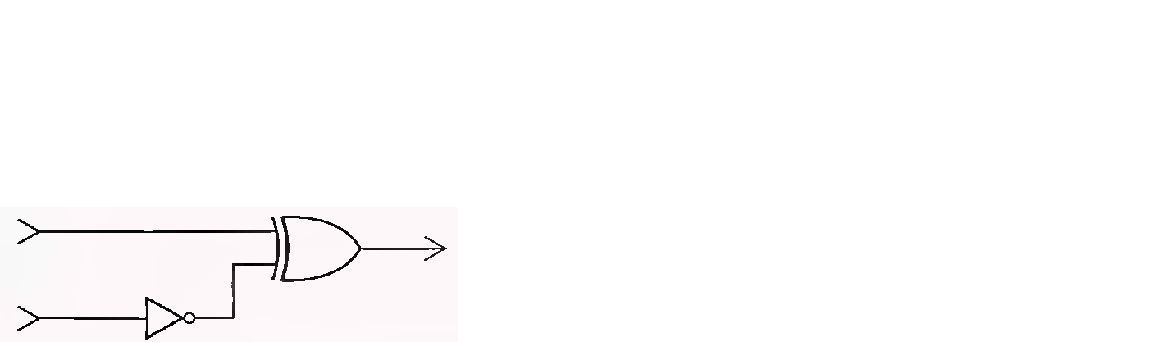
\includegraphics{ch2/ex21a.pdf}}

    \item \scalebox{0.6}{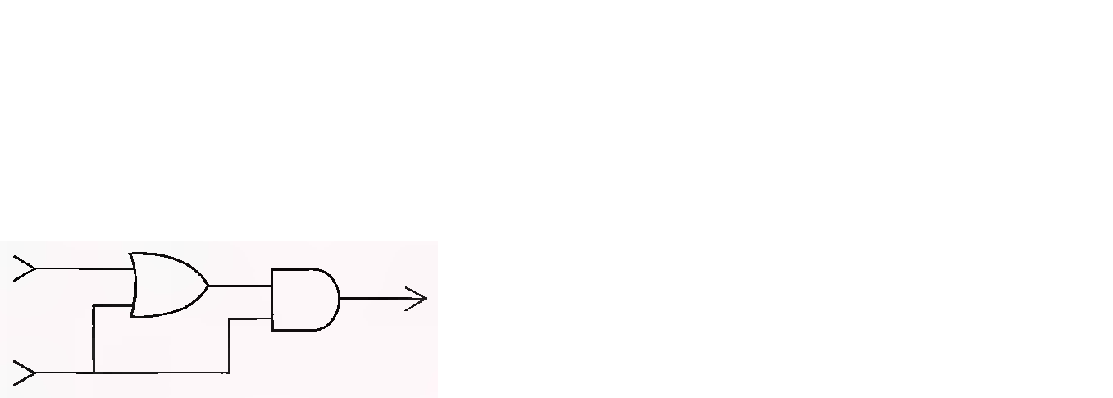
\includegraphics{ch2/ex21b.pdf}}

    \item \scalebox{0.6}{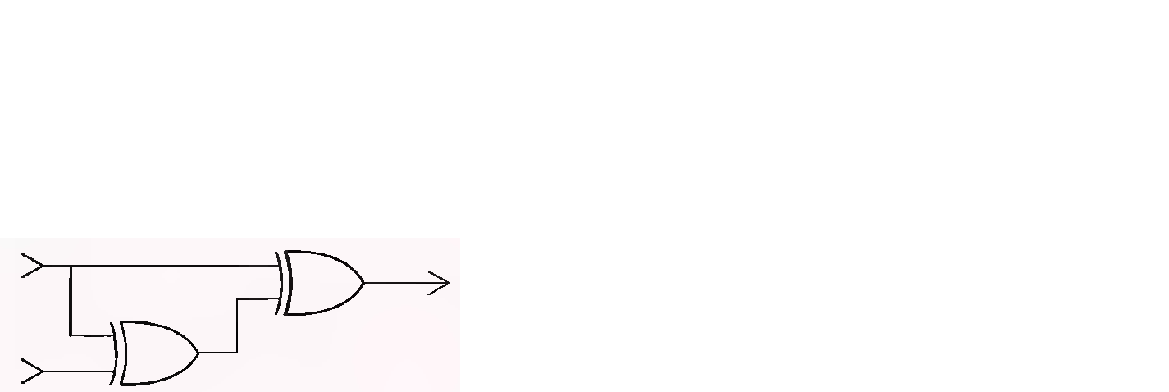
\includegraphics{ch2/ex21c.pdf}}
    \end{enumerate}
  \item Với mỗi mạch dưới đây, hãy xác định các tổ hợp đầu vào để đầu ra là $1$.
    \begin{enumerate}
    \item \scalebox{0.6}{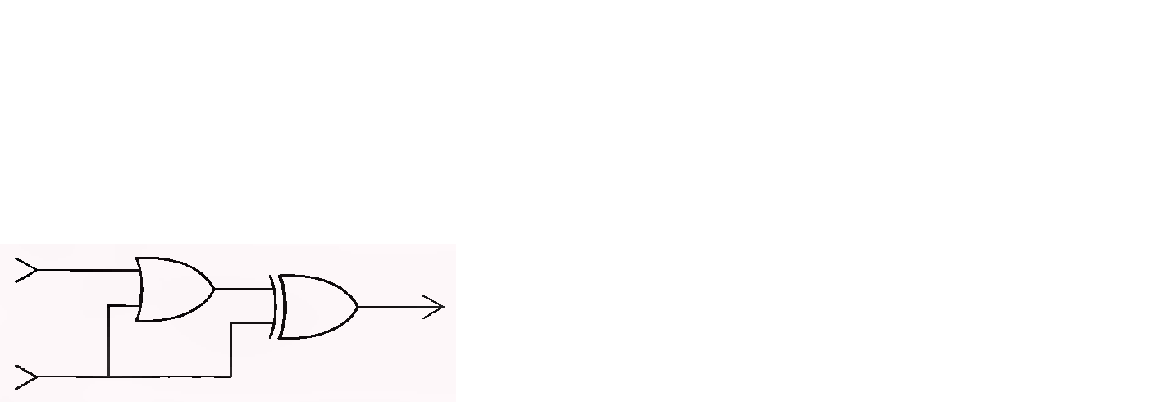
\includegraphics{ch2/ex22a.pdf}}

    \item \scalebox{0.6}{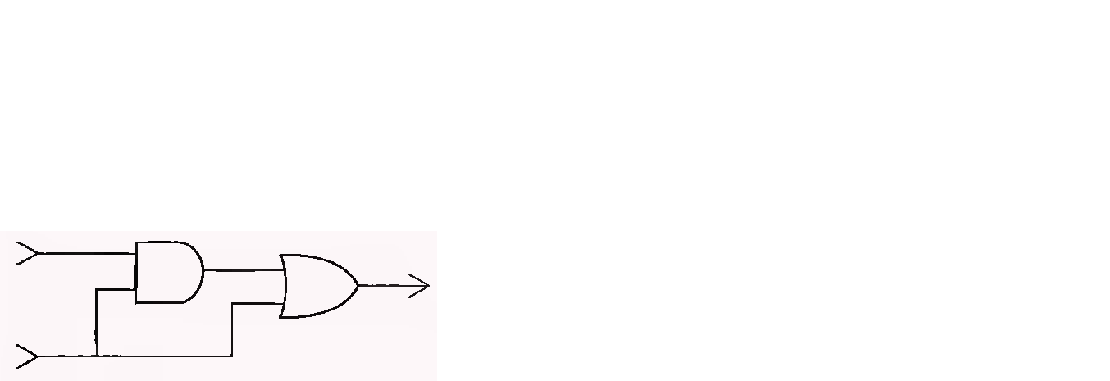
\includegraphics{ch2/ex22b.pdf}}

    \item \scalebox{0.6}{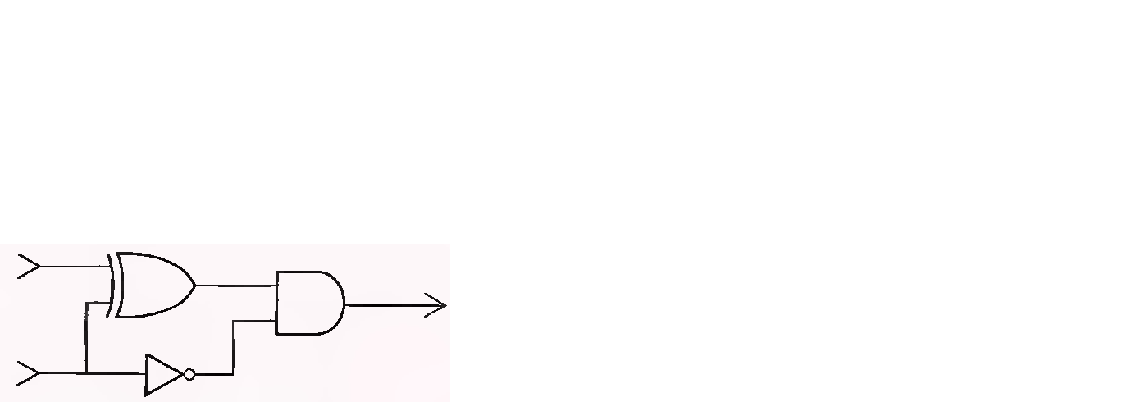
\includegraphics{ch2/ex22c.pdf}}

    \end{enumerate}

  \item Trong mỗi mạch dưới đây, các hình chữ nhật biểu diễn cùng một loại cổng. Dựa vào
    thông tin đầu vào và đầu ra, hãy xác định cổng liên quan trong hình là $\AND$, $\OR$
    hay $\XOR$.
    \begin{enumerate}
    \item \scalebox{0.6}{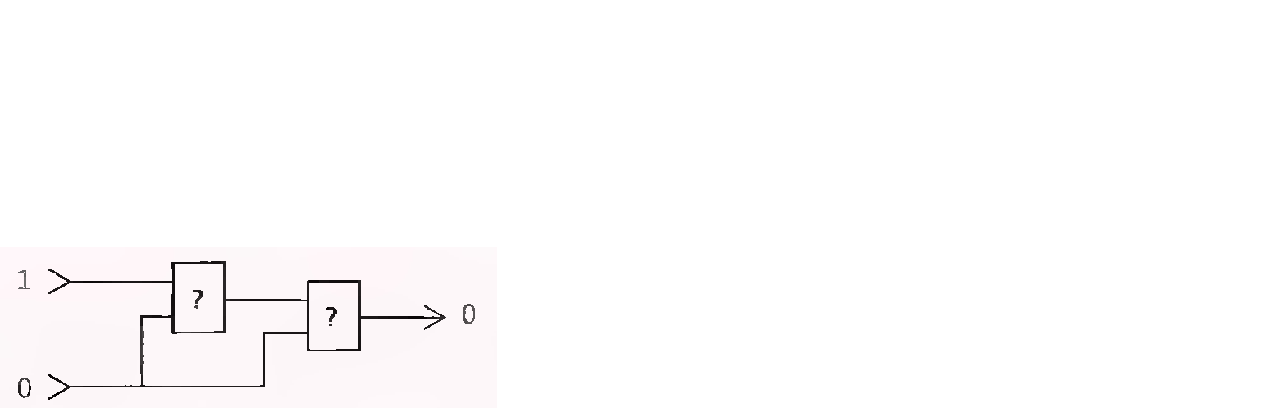
\includegraphics{ch2/ex23a.pdf}}

    \item \scalebox{0.6}{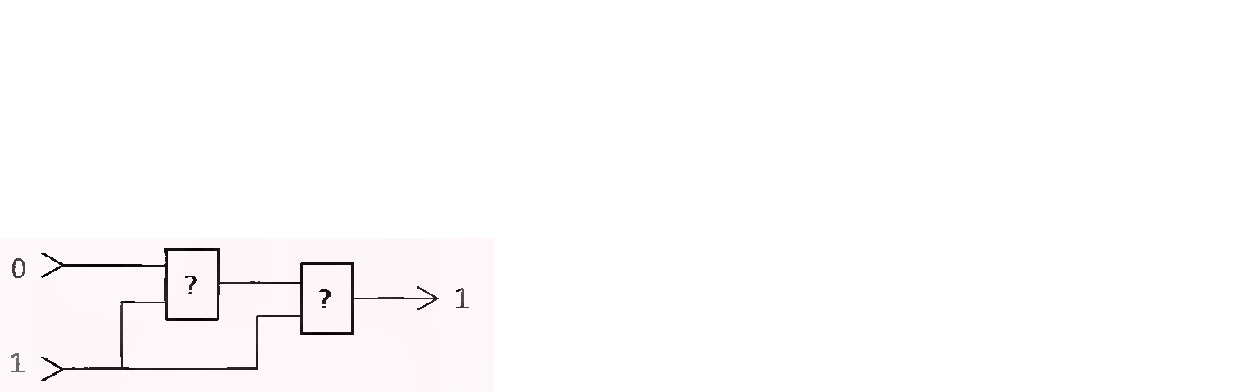
\includegraphics{ch2/ex23b.pdf}}

    \item \scalebox{0.6}{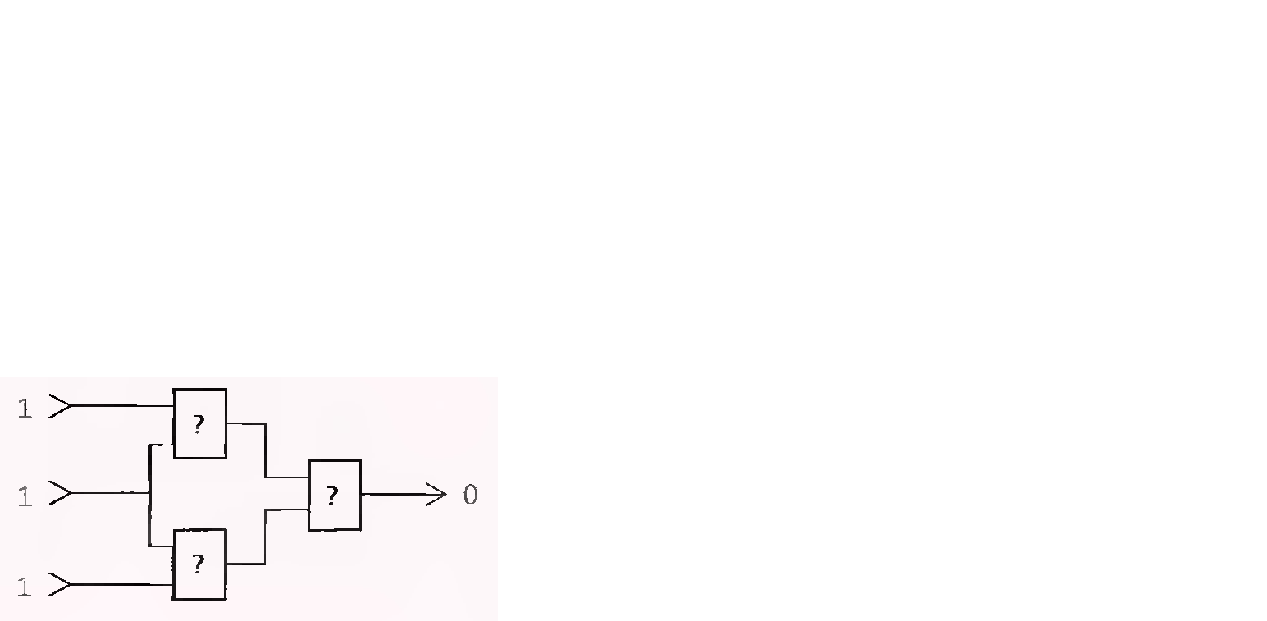
\includegraphics{ch2/ex23c.pdf}}

    \end{enumerate}

  \item Giả sử rằng cả đầu vào và đầu ra trong mạch dưới đây là $1$. Mô tả xem chuyện gì
    xảy ra nếu đầu vào phía trên tạm thời thay đổi về $0$. Mô tả xem chuyện gì xảy ra nếu
    đầu vào phía dưới tạm thời thay đổi về $0$. Vẽ lại mạch sử dụng các cổng $\NAND$.
    \begin{center}
      \scalebox{0.7}{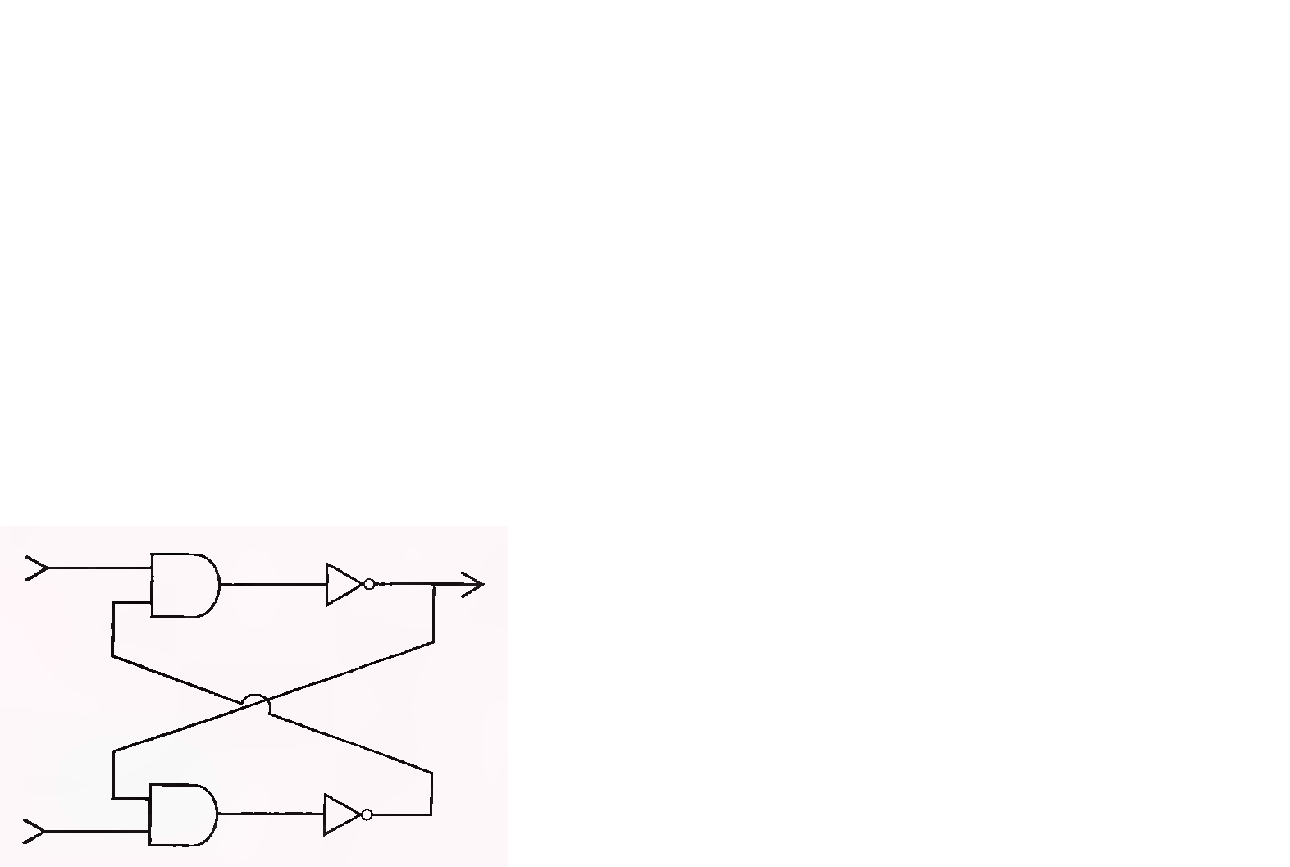
\includegraphics{ch2/ex24.pdf}}
    \end{center}
  \item Bảng dưới đây biểu diễn địa chỉ và nội dung (dùng ký hiệu hexa) của một vài ô nhớ
    trong bộ nhớ chính của máy tính. Hãy thực hiện theo dãy các lệnh ở dưới đây và ghi lại
    nội dung của các ô nhớ này.

    \begin{tabular}[c]{cc}
      Địa chỉ & Nội dung \\
      $00$ & $AB$ \\
      $01$ & $53$ \\
      $02$ & $D6$ \\
      $03$ & $02$
    \end{tabular}
    \begin{enumerate}[B1. ]
    \item Chuyển nội dung của ô nhớ có địa chỉ là $03$ vào ô nhớ địa chỉ~$00$.

    \item Chuyển giá trị $01$ vào ô nhớ tại địa chỉ $00$.

    \item Chuyển giá trị được lưu trữ tại địa chỉ $01$ vào ô nhớ tại địa chỉ~$03$.
    \end{enumerate}

  \item Nếu địa chỉ mỗi ô nhớ của một máy được biểu diễn bởi hai số hexa, vậy có bao nhiêu
    ô nhớ trong bộ nhớ chính của máy tính này?  có bao nhiêu ô nhớ nếu mỗi ô nhớ biểu diễn
    bởi bốn số hexa?

  \item Xâu bít gì được biểu diễn bởi ký hiệu hexa sau đây?

    \begin{inparaenum}[a.]
    \item $CB$ \quad
    \item $67$ \quad
    \item $A9$ \quad
    \item $10$ \quad
    \item $FF$
    \end{inparaenum}

  \item Giá trị của bít trọng số cao nhất trong xâu bít được biểu diễn bởi các ký hiệu
    hexa sau đây là gì?

    \begin{inparaenum}[a.]
    \item $7F$ \quad
    \item $FF$ \quad
    \item $8F$ \quad
    \item $1F$
    \end{inparaenum}

  \item Biểu diễn các xâu bít dưới đây thành ký hiệu hexa:
    \begin{enumerate}[a.]
    \item $101010101010$
    \item $110010110111$
    \item $000011101011$
    \end{enumerate}

  \item Giả sử một camera số có một khả năng lưu trữ là $256$MB. Có bao nhiêu bức ảnh có
    thể được lưu trữ trong camera nếu mỗi ảnh bao gồm $1024$ điểm ảnh trên một dòng và
    $1024$ điểm ảnh trên một cột và nếu mỗi điểm ảnh cần ba byte để lưu trữ.

  \item Giả sử một bức ảnh được biểu diễn trên màn hình máy tính bởi một mảng hình chữ
    nhật chứa $1024$ cột và $768$ dòng điểm ảnh. Nếu tám bít yêu cầu để mã hoá màu và
    cường độ của mỗi điểm ảnh, vậy cần bao nhiêu ô nhớ (tính theo byte) để lưu trữ được
    toàn bộ bức ảnh này.

  \item \begin{enumerate}[a.]
    \item Chỉ ra hai ưu điểm của bộ nhớ chính so với đĩa từ.
    \item Chỉ ra hai ưu điểm của đĩa từ so với bộ nhớ chính.
    \end{enumerate}

  \item Giả sử bạn chỉ còn $50$GB trống trong ổ đĩa cứng $120$GB của bạn. Có hợp lý không
    khi bạn định dùng các đĩa CD để lưu trữ toàn bộ dữ liệu trên ổ như dữ liệu backup? Có
    hợp lý không khi dùng DVD?

  \item Nếu mỗi sector trên đĩa từ chứa $1024$ byte, ta cần bao nhiêu sector để lưu trữ
    một trang văn bản (mỗi trang chứa khoảng $50$ dòng, mỗi dòng khoảng $100$ ký tự) và
    mỗi ký tự được biểu diễn dùng Unicode?

  \item Ta cần bao nhiêu byte để lưu trữ $400$ trang ở đó mỗi trang lưu trữ $3500$ nếu ký
    tự được mã hoá dùng ASCII? Cần bao nhiêu byte nếu mỗi ký tự biểu diễn ở dạng Unicode?

  \item Thời gian trễ của một đĩa cứng là bao nhiêu nếu nó quay với tốc độ $60$ vòng trên
    giây?

  \item Thời gian truy cập trung bình của đĩa cứng là bao nhiêu nếu nó quay với tốc độ
    $60$ vòng trên giây và thời gian dịch chuyển là $10$ milli giây?

  \item Giả sử một người đánh máy có thể đánh được $60$ từ trong một phút liên tục từ ngày
    này sang ngày khác. Để số ký tự đã đánh lưu vào được đầy một đĩa CD kích thước
    $640$MB, người này cần đánh máy trong bao lâu? (giả sử một từ gồm năm ký tự và mỗi ký
    tự cần một byte để lưu trữ.)

  \item Đây là một bức thông điệp ở dạng ASCII. Hãy giải mã xem nó nói
    gì? \\
    \texttt{01010111 01101000 01100001 01110100 00100000 01100100 01101111 01100101
      01110011 00100000 01101001 01110100 00100000 01110011 01100001 01111001 00111111}

  \item Thông điệp dưới đây được mã hoá dưới dạng ASCII dùng một byte cho mỗi ký tự và
    được biểu diễn dùng ký hiệu hexa. Thông điệp sau
    đây muốn nói gì?
    \begin{center}
      $68657861646563696D616C$
    \end{center}
  \item Mã hoá các câu sau đây dưới dạng mã ASCII dùng một byte một ký tự.
\label{ex:221}
    \begin{enumerate}[a.]
    \item $100/5=20$
    \item To be or not to be?
    \item The total cost is \$$7.25$.
    \end{enumerate}
 
  \item Biểu diễn các câu trả lời của bài \ref{ex:221} dưới dạng ký hiệu hexa.

  \item Liệt kê các biểu diễn nhị phân của các số nguyên từ $6$ tới $16$.

  \item \begin{enumerate}[a.]
    \item Viết số $26$ bằng cách biểu diễn $2$ và $6$ ở dạng ASCII.

    \item Viết số $26$ ở dạng biểu diễn nhị phân.
    \end{enumerate}

  \item Những giá trị nào trong biểu diễn nhị phân chỉ có một trong các bít bằng~$1$? Liệt
    kê các biểu diễn nhị phân cho sáu giá trị nhỏ nhất với tính chất này.

  \end{enumerate}

\end{multicols}



%%% Local Variables: 
%%% mode: latex
%%% TeX-master: "../tindaicuong"
%%% End: 

%%% Local Variables: 
%%% mode: latex
%%% TeX-master: "../tindaicuong"
%%% End: 
 

\chapter{Thao tác dữ liệu}
\label{chap:ch3}

\minitoc
\vspace{0.5cm}
\noindent
Trong chương này, ta sẽ xem xét cách máy tính thao tác với dữ liệu và giao tiếp với thiết
bị ngoại vi như máy in và bàn phím. Để làm điều đó, ta sẽ xem xét cơ bản về kiến trúc máy
tính, chỉ ra làm thế nào để lập trình bằng cách mã hoá các lệnh (ở mức máy).


\section{Kiến trúc máy tính}
Phần mạch điện trong máy tính điều khiển các thao tác trên dữ liệu gọi là \textbf{đơn vị
  xử lý trung tâm}, hay CPU - Center Processing Unit.  Người ta thường ví nó như là "bộ
não" của máy tính.
 

Một CPU bao gồm hai phần: \textbf{đơn vị tính toán số học/logic}, hay ALU (viết tắt của
Arthmetic/Logic Unit) và \textbf{đơn vị điều khiển} (control unit). Phần ALU gồm các mạch
thực hiện các phép toán trên dữ liệu (như cộng hoặc trừ). Còn đơn vị điều khiển gồm các
mạch để điều phối các hoạt động của máy. Ngoài ra, để lưu trữ các thông tin trung gian,
CPU còn chứa một tập các ô nhớ, gọi là \textbf{thanh ghi}, tương tự như các ô nhớ của bộ
nhớ chính. Các thanh ghi này được chia làm hai loại: \textbf{thanh ghi đa năng}
(general-purpose registers) và \textbf{thanh ghi chuyên dụng} (special-purpose
registers). Dưới đây, ta xem xét thanh ghi đa năng, còn các thanh ghi chuyên dụng sẽ được
thảo luận trong Mục~\ref{sec:2.3}.

\begin{figure}
  \centering \scalebox{0.6}{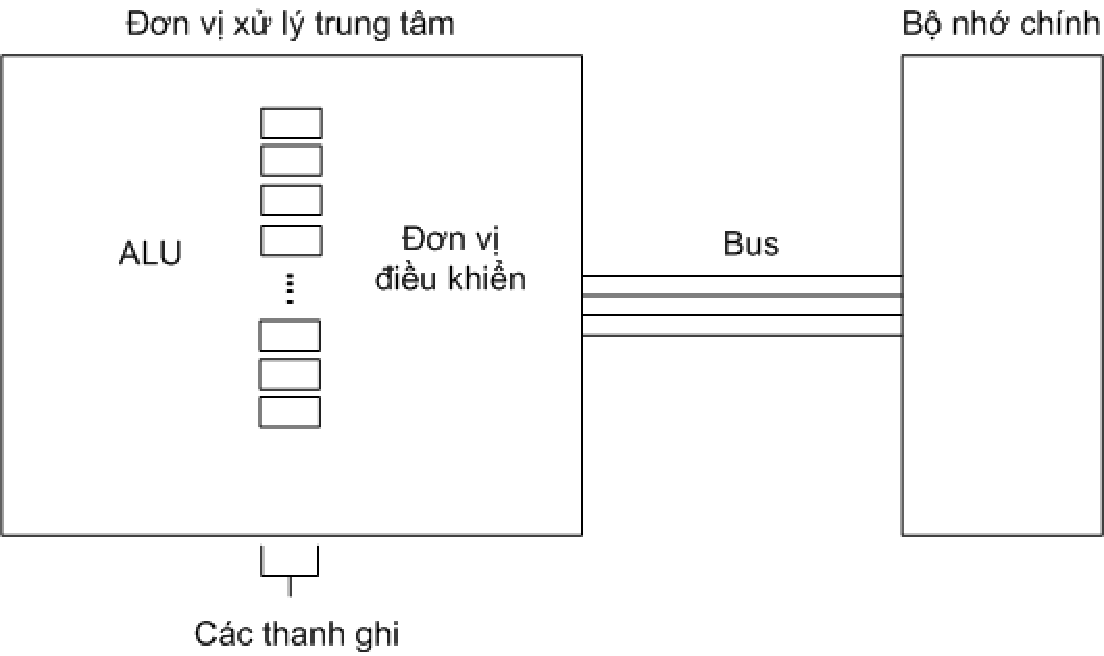
\includegraphics{ch3/fig21.pdf}}
  \caption{CPU và bộ nhớ chính kết nối với nhau thông qua một bus}
  \label{fig:fig21}
\end{figure}

Thanh ghi đa năng dùng để lưu trữ các dữ liệu tạm thời trong khi CPU thực hiện tính
toán. Các thanh ghi này vừa lưu trữ giá trị đầu vào, vừa lưu trữ kết quả sau khi tính toán
của ALU. Để thực hiện một phép toán liên quan đến dữ liệu trong bộ nhớ chính, đơn vị điều
khiển phải chuyển dữ liệu từ bộ nhớ vào các thanh ghi đa năng, thông báo cho ALU biết
thanh ghi nào lưu trữ dữ liệu, kích hoạt mạch thích hợp trong ALU, và thông báo cho ALU
thanh ghi nào để lưu trữ kết quả.      


Để chuyển dữ liệu (dãy bít), CPU và bộ nhớ chính được liên kết với nhau bởi nhiều dây nối,
thường gọi là các \textbf{bus} (xem Hình~\ref{fig:fig21}). Nhờ các bus này, CPU có thể lấy
(đọc) dữ liệu từ bộ nhớ chính bằng cách cung cấp hai thông tin: \begin{inparaenum}[(1)]
\item địa chỉ ô nhớ cần đọc;
\item một tín hiệu đặc biệt thông báo với bộ nhớ gửi dữ liệu cho nó.
\end{inparaenum}
Tương tự, CPU ghi dữ liệu vào bộ nhớ bằng cách cung cấp ba thông
tin: \begin{inparaenum}[(1)]
\item địa chỉ của ô nhớ cần ghi; 
\item dữ liệu cần ghi;
\item một tín hiệu đặc biệt thông báo với bộ nhớ ghi dữ liệu mà nó gửi đến.
\end{inparaenum}

Dựa trên cách thiết kế này, việc cộng hai giá trị nằm trong bộ nhớ chính sẽ không phải chỉ
là thực hiện phép cộng. Thực vậy, để thực hiện thao tác cộng này, nó phải hoàn thành đầy
đủ năm bước liệt kê trong Hình~\ref{fig:fig22}. Tóm lại, các thao tác bao gồm: dữ liệu được
chuyển từ bộ nhớ chính tới các thanh ghi bên trong CPU, sau đó ALU thực hiện cộng giá trị
của các thanh ghi này, và cuối cùng đặt giá trị của thanh ghi kết quả vào trong một ô nhớ
trong bộ nhớ chính.
 
\begin{figure}[tb]
  \centering
  \begin{tabular}{m{1.5cm}m{9cm}}
    Bước $1$. & Lấy toán hạng thứ nhất  từ  trong bộ nhớ và đặt vào các thanh   ghi.\\ \\

    Bước $2$. & Lấy toán hạng thứ hai  từ trong bộ nhớ và đặt nó vào một thanh ghi   khác.   \\  \\

    Bước $3$. & Kích hoạt mạch cộng với đầu vào là các thanh ghi trong các Bước $1$ và
    $2$, và dùng  một thanh ghi khác để lưu kết quả. \\ \\

    Bước $4$. & Lưu giữ kết quả vào trong bộ nhớ. \\ \\

    Bước $5$. & Dừng chương trình. 
  \end{tabular}
  \caption{Cộng các giá trị trong bộ nhớ}
  \label{fig:fig22}
\end{figure}


Các máy tính trước đây rất khó khăn khi thực hiện các công việc khác nhau, vì đối với mỗi
việc, các bước thực hiện phải được xây dựng sẵn trước trong đơn vị điều khiển như một phần
của máy. Để có được tính mềm dẻo, các thiết bị điện trước đây được thiết kế sao cho có thể
dễ dàng nối lại dây tương ứng cho mỗi nhiệm vụ. Trước khi thực hiện một nhiệm vụ các dây
nối phải được cắm sẵn vào trong các lỗ cắm thích hợp. Cách thiết kế này giống như chuyển
mạch trong các hệ thống điện thoại đời cũ.

Mọi vấn đề được giải quyết nhờ vào ý tưởng mang tính đột phá của Von Neumann. Ông đã chỉ
ra rằng chương trình cũng là một loại dữ liệu, nó được mã hoá và lưu trong bộ nhớ
chính. Nếu đơn vị điều khiển được thiết kế để đọc lệnh từ bộ nhớ, giải mã lệnh, và thực
hiện lệnh, thì thay vì phải nối lại dây để thay đổi chương trình máy tính, ta chỉ phải đặt
nội dung của một vài ô nhớ tương ứng với chương trình.

Ý tưởng về chương trình được đặt trong bộ nhớ chính được gọi là \textbf{khái niệm lưu trữ
  chương trình}. Ngày nay, nó trở thành cách tiếp cận chính thống - nó quen thuộc tới mức
đã trở nên hiển nhiên trong việc thiết kế máy tính. Thực chất, những khó khăn của thời kỳ
trước là do mọi người đã quen với việc phân biệt chương trình và dữ liệu như những thực
thể khác nhau: dữ liệu được lưu trữ trong bộ nhớ, còn chương trình phải là một phần của
đơn vị điều khiển. Đây là một ví dụ điển hình cho thấy lợi ích khi thay đổi cách tư duy.

\subsection*{Câu Hỏi \& Bài tập}

\begin{enumerate}
\item Bạn hãy chỉ ra dãy các hoạt động cần thiết để chuyển dữ liệu từ một ô nhớ này tới
  một ô nhớ khác trong máy tính?

\item Để có thể ghi một giá trị vào ô nhớ, CPU phải cung cấp cho bộ nhớ chính những thông
  tin gì?

\item Thiết bị lưu trữ khối, bộ nhớ chính, và thanh ghi đa năng đều là các hệ thống lưu
  trữ. Hãy chỉ ra sự khác nhau trong cách sử dụng của chúng?

\end{enumerate}

\section{Ngôn ngữ máy}
Để áp dụng được khái niệm lưu trữ chương trình, các CPU được thiết kế để đoán nhận các
lệnh được mã hoá dưới dạng các dãy bít. Tập các lệnh cùng với cách mã hoá được gọi là
\textbf{ngôn ngữ máy}. Các lệnh biểu thị trong ngôn ngữ này được gọi là lệnh ở mức máy,
hay ngắn gọn là \textbf{lệnh máy}.

\subsection*{Tập lệnh}
Danh sách các lệnh mà một CPU điển hình có thể giải mã và thực hiện được khá ngắn. Khi mà
một máy đã có thể thực hiện một số nhiệm vụ cơ bản và được lựa chọn hợp lý, việc thêm vào
một số đặc điểm, về mặt lý thuyết, sẽ không làm tăng khả năng của máy. Nói cách khác, việc
thêm những đặc điểm này chỉ làm máy thêm thích hợp với người sử dụng, chứ không tăng chức
năng cơ bản của nó.

Có hai quan điểm về kiến trúc CPU. Một quan điểm cho rằng CPU nên được thiết kế chỉ có một
số tối thiểu các lệnh máy cần thiết. Cách tiếp cận này dẫn tới khái niệm \textbf{kiến trúc
  tập lệnh rút gọn} (RISC - reduced instruction set computer). Ưu điểm của kiến trúc RISC
là máy thực hiện hiệu quả và nhanh chóng do tính đơn giản của tập lệnh.

Quan điểm khác cho rằng CPU nên có sẵn một tập lớn các lệnh phức tạp, dù chúng có dư thừa
về mặt kỹ thuật. Kết quả cách tiếp cận này là \textbf{kiến trúc tập lệnh phức tạp} (CISC -
reduced instruction set computer).  Luận điểm của kiến trúc CISC là nếu CPU phức tạp có
nghĩa là việc viết chương trình trên đó sẽ đơn giản.  Bởi vậy, để thực hiện một lệnh phức
tạp ở kiến trúc CISC nói chung cần thực hiện nhiều lệnh ở kiến trúc RISC.

Cả hai loại bộ xử lý RISC và CISC đều có sẵn trên thị trường. Dòng xử lý Pentium, được
phát triển bởi Intel, là một ví dụ về kiến trúc CISC. Dòng PowerPC (bao gồm các bộ xử lý
mà Apple gọi là G4 và G5), được phát triển bởi Apple, IBM và Motorola là ví dụ về kiến
trúc RISC.  (Apple hiện nay sản xuất máy dựa trên sản phẩm của Intel. Tuy nhiên, việc
chuyển đổi này là vì lý do thương mại, chứ không phải là do phân biệt ưu nhược điểm của
triết lý thiết kế RISC và CISC).

Dù ở kiến trúc RISC hay CISC, một lệnh máy vẫn có thể được phân loại thành ba
nhóm: \begin{inparaenum}[(1)]
\item nhóm lệnh chuyển dữ liệu;
\item nhóm lệnh số học và logic;
\item nhóm lệnh điều khiển.
\end{inparaenum}

\paragraph{Chuyển dữ liệu} Nhóm chuyển dữ liệu bao gồm các lệnh yêu cầu chuyển dữ liệu từ
ô nhớ này sang ô nhớ khác. Các bước 1, 2, và 4 trong Hình \ref{fig:fig22} là loại lệnh
này. Ta nên để ý rằng việc sử dụng thuật ngữ \textit{chuyển} ở đây không hoàn toàn chính
xác. Rất hiếm khi dữ liệu được chuyển đi bằng cách sao chép sang ô nhớ mới đồng thời xoá ở
ô nhớ gốc. Lệnh chuyển ở đây giống như việc sao chép dữ liệu hơn. Bởi vậy nên mô tả hoạt
động của nhóm lệnh này bằng thuật ngữ sao chép thay vì chuyển.

Cũng liên quan đến thuật ngữ, ta thảo luận hai thuật ngữ đặc biệt thường dùng cho thao tác
chuyển dữ liệu giữa CPU và bộ nhớ chính: đó là LOAD và STORE. Yêu cầu đặt giá trị cho
thanh ghi đa năng bằng nội dung của ô nhớ thường được gọi là lệnh LOAD.  Ngược lại, yêu
cầu chuyển nội dung của thanh ghi vào trong một ô nhớ được gọi là STORE. Trong hình
\ref{fig:fig22}, Bước 1 và 2 là lệnh LOAD, và bước 4 là lệnh STORE.

Một nhóm con quan trọng trong nhóm lệnh chuyển dữ liệu là các lệnh giao tiếp với thiết bị
ngoại vi (như máy in, bàn phím, màn hình, bộ điều khiển đĩa,...). Bởi vì các lệnh này thực
hiện các hoạt động vào/ra (I/O) của máy, nên chúng được gọi là lệnh I/O. Thực chất, các
lệnh này được thực hiện nhờ vào các lệnh chuyển dữ liệu giữa CPU và bộ nhớ, ta sẽ giải
thích chi tiết cách làm trong Mục~\ref{sec:2.5}. Vì vậy, ta cũng xếp các lệnh I/O vào nhóm
lệnh chuyển dữ liệu.

\paragraph{Số học và logic} Nhóm số học và logic gồm các lệnh nhằm thông báo với bộ điều
khiển yêu cầu một hoạt động xử lý bởi đơn vị tính toán số học và logic. Bước 3 trong hình
\ref{fig:fig22} rơi vào nhóm này. Giống như tên gọi, đơn vị số học và logic không chỉ có khả
năng thực hiện các phép toán số học, mà còn nhiều phép toán khác nữa.  Một số trong đó là
các phép toán Boolean $\AND$, $\OR$ và $\XOR$ như được giới thiệu trong Chương~\ref{chap:chuong1}.

Ngoài ra, một tập các phép toán khác sẵn có trong hầu hết các đơn vị số học và logic cho
phép dịch nội dung thanh ghi sang phải hoặc trái. Các phép toán này được biết như các phép
toán SHIFT hoặc ROTATE. Sự khác biệt giữa hai lệnh này là, đối với lệnh SHIFT thì bít ``ở
vị trí cuối cùng'' của thanh ghi bị bỏ qua, còn với ROTATE thì bít này được quay vòng lại
phía đầu bên kia của thanh ghi.

\paragraph{Điều khiển} Nhóm lệnh điều khiển bao gồm các lệnh trực tiếp thực hiện chương
trình thay vì thao tác dữ liệu. Bước 5 trong Hình \ref{fig:fig22} thuộc nhóm lệnh
này. Nhóm lệnh này chứa nhiều lệnh rất quan trọng trong tập lệnh máy, như họ các lệnh nhảy
JUMP (hoặc BRANCH) được sử dụng để thay đổi thứ tự thực hiện lệnh. Nó cho phép chuyển đến
thực hiện một lệnh bất kỳ, thay vì thực hiện lệnh tiếp theo trong danh sách lệnh. Có hai
kiểu lệnh JUMP: \textbf{lệnh nhảy không điều kiện} và \textbf{lệnh nhảy có điều kiện}. Một
ví dụ của kiểu lệnh nhảy không điều kiện là ``Nhảy tới Bước 5''; một ví dụ của kiểu lệnh
nhảy có điều kiện là ``Nếu giá trị đạt được là 0, vậy nhảy tới Bước 5''. Sự khác biệt giữa
các lệnh này là lệnh nhảy có điều kiện thực hiện ``thay đổi nơi đến'' chỉ nếu một số điều
kiện được thoả mãn. Như một ví dụ, dãy các lệnh trong Hình~\ref{fig:fig23} biểu diễn thuật
toán chia hai giá trị ở đó Bước 3 là điều kiện nhảy có điều kiện nhằm tránh trường hợp
chia cho không.

\begin{figure}[tb]
  \begin{center}
    \begin{tabular}{m{2cm}m{7cm}}
      Bước $1$. & LOAD một thanh ghi với một giá trị từ bộ nhớ.         \\   \\

      Bước $2$. & LOAD thanh ghi khác với giá trị khác trong bộ nhớ.    \\   \\

      Bước $3$. & Nếu giá trị thứ hai này bằng không,                   \\
      & JUMP tới Bước $6$.                                    \\   \\

      Bước $4$. & Chi nội dung của thanh ghi đầu tiên với thanh ghi thứ hai   và đặt kết quả vào thanh ghi thứ ba.                              \\   \\

      Bước $5$. & STORE nội dung của thanh ghi thứ ba vào trong bộ nhớ. \\   \\

      Bước $6$. & STOP.
    \end{tabular}
  \end{center}
  \caption{Chia các giá trị trong bộ nhớ}
  \label{fig:fig23}

\end{figure}

\subsection*{Một mô tả ngôn ngữ máy}
Ta sẽ cùng xem xét cách mã hoá các lệnh của một máy tính. Máy mà ta sẽ sử dụng cho thảo
luận sẽ được mô tả trong Phụ lục~\ref{phuluc1} và được tóm tắt trong
Hình~\ref{fig:fig24}. Máy này gồm~$16$ thanh ghi đa năng và bộ nhớ chính gồm $256$ ô nhớ,
mỗi ô nhớ có khả năng lưu trữ tám bít. Để tiện tham chiếu, ta gán nhãn các thanh ghi bởi
các giá trị từ $0$ tới $15$ và địa chỉ của các ô nhớ từ $0$ tới $255$. Để tiện lợi, ta xem
các nhãn và địa chỉ này như các giá trị nhị phân và viết gọn dưới dạng hexa. Và do đó, các
thanh ghi được gán nhãn từ $0$ tới $F$, và các ô nhớ được đánh địa chỉ từ $00$ tới $FF$.

\begin{figure}[tbh]
  \centering \scalebox{0.6}{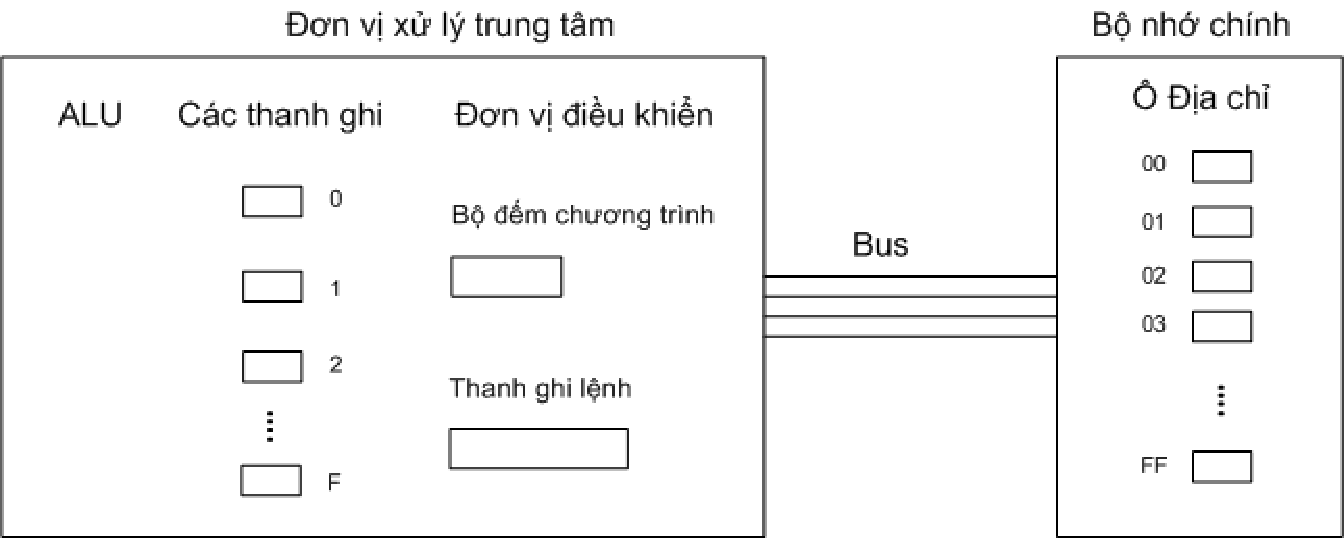
\includegraphics{ch3/fig24.pdf}}
  \caption{Kiến trúc máy được mô tả trong Phụ lục \ref{phuluc1}}
  \label{fig:fig24}
\end{figure}

Các lệnh máy được mã hoá gồm hai phần: trường \textbf{op-code} (viết tắt của mã toán tử)
và trường \textbf{toán hạng}. Dãy bít xuất hiện trong phần op-code chỉ ra phép toán nào
được thực hiện, kiểu như STORE, SHIFT, XOR, và JUMP; và trường này bắt buộc phải có trong
mọi lệnh. Dãy bít trong trường toán hạng cung cấp các thông tin chi tiết về phép toán được
xác định bởi op-code. Ví dụ với phép toán STORE, thông tin trong trường toán hạng chỉ
ra: \begin{inparaenum}[(1)]
\item thanh ghi nào chứa dữ liệu cần ghi;
\item và ô nhớ nào để nhận dữ liệu. 
\end{inparaenum}

Ngôn ngữ máy mô tả ở Phục lục \ref{phuluc1} chỉ gồm $12$ lệnh cơ bản. Mỗi lệnh được mã hoá
bằng $16$ bít, và biểu diễn bởi một số thập lục phân gồm bốn chữ số
(Hình~\ref{fig:fig25}). Trong đó, bốn bít đầu tiên là phần op-code, hay tương đương chữ số
dầu tiên của số thập lục phân. Để ý (Phụ lục \ref{phuluc1}) rằng các op-code này được biểu
diễn bởi các chữ số hexa từ $1$ tới~$C$. Đặc biệt, Bảng trong Phụ lục \ref{phuluc1} chỉ
cho ta rằng một lệnh bắt đầu bằng chữ số $3$ (ở dạng hexa) tham chiếu đến lệnh STORE, lệnh
bắt đầu bằng chữ số $A$ tham chiếu đến lệnh ROTATE.

\begin{figure}[bth] 
  \centering \input{ch3/fig25}
  \caption{Các thành phần của một lệnh máy trong Phụ lục \ref{phuluc1}}
  \label{fig:fig25}
\end{figure}


Trường toán hạng của mỗi lệnh trong mô tả máy của ta bao gồm ba chữ số hexa~(12 bít), và
ngoại trừ lệnh HALT không cần thông tin gì thêm, nó sẽ làm rõ xem lệnh đưa bởi op-code
phải làm gì. Ví dụ, xem Hình~\ref{fig:fig26}, nếu chữ số hexa đầu tiên của một lệnh là $3$
chỉ ra đây là lệnh lưu trữ nội dung của thanh ghi vào bộ nhớ, số hexa tiếp theo của lệnh
chỉ ra thanh ghi nào cần lưu trữ, và hai số hexa cuối chỉ ra ô nhớ nào dùng để lưu dữ
liệu. Bởi vậy lệnh $35A7$ (ở dạng hexa) dịch thành lệnh ``STORE mẫu bít tìm thấy trong
thanh ghi 5 vào trong ô nhớ có địa chỉ là A7''. Chú ý rằng việc sử dụng ký hiệu hexa giúp
ta đơn giản trong việc nhìn các lệnh. Còn trên thực tế, lệnh $35A7$ là dãy
bít~$0011010110100111$.
 

%\begin{wrapfigure}{r}{90mm}
\begin{figure}[thb]
  \centering \input{ch3/fig26}
  \caption{Giải mã lệnh $35A7$}
  \label{fig:fig26}
\end{figure}
%\end{wrapfigure}

Lệnh $35A7$ cũng cung cấp một ví dụ rõ ràng tại sao dung lượng bộ nhớ chính được tính theo
luỹ thừa của hai. Bởi vì tám bít trong lệnh để dành cho việc xác định ô nhớ nào được sử
dụng trong lệnh, nó có khả năng tham khảo tới chính xác $2^8$ ô nhớ khác nhau. Bởi thế ta
cần xây dựng bộ nhớ có đúng số ô nhớ như thế--đánh địa chỉ từ $0$ tới $255$. Nếu bộ nhớ
chính có nhiều ô nhớ hơn, thì số ta không thể viết lệnh phân biệt chúng; còn nếu có ít ô
nhớ hơn, có trường hợp ta viết lệnh tham chiếu đến một ô nhớ không tồn tại.


Một ví dụ khác chỉ ra xem làm thế nào trường toán hạng được sử dụng để làm rõ lệnh xác
định bởi op-code. Ta xét lệnh có op-code $7$ (ở dạng hexa), lệnh này yêu cầu $\OR$ nội
dung của hai thanh ghi với nhau (ta sẽ giải thích làm thế nào để $\OR$ hai thanh ghi sau,
trong Mục~\ref{sec:2.4}). Bây giờ ta chỉ đơn thuần quan tâm xem làm thế nào lệnh được mã
hoá. Trong trường hợp này, chữ số hexa tiếp theo chỉ ra thanh ghi nào sẽ được lưu kết quả,
còn hai số hexa cuối chỉ ra hai thanh ghi nào sẽ được $\OR$ với nhau. Bởi vậy lệnh~$70C5$
được dịch thành ``OR nội dung của thanh ghi $C$ với nội dung của thanh ghi $5$ và đặt kết
quả vào thanh ghi $0$''.

Ta cũng cần phân biệt giữa hai lệnh máy LOAD. Ở đây ta, lệnh có op-code $1$ (ở dạng hexa)
là lệnh nạp giá trị là nội dung của một ô nhớ vào một thanh ghi, trong khi đó op-code $2$
(ở dạng hexa) là lệnh nạp một hằng số vào thanh ghi. Sự khác biệt ở đây là, với lệnh nạp
kiểu đầu tiên, trường toán hạng chứa một địa chỉ; trong khi đó, với lệnh nạp kiểu thứ hai,
trường toán hạng là dãy bít cần được được nạp.

Để ý rằng máy có hai lệnh ADD, một để cộng hai số biểu diễn bù hai và một để cộng biểu
diễn dấu chấm động. Sự phân biệt này là hậu quả của sự kiện rằng, bên trong đơn vị số học
và logic, cách hoạt động để cộng các số được mã hoá ở dạng bù hai khác với cách cộng các
số mã hoá theo ký hiệu dấu chấm động .

\begin{figure}[thb]
  \centering
  \begin{tabular}{m{2.5cm}m{7cm}}
    \textbf{Lệnh}   & \textbf{Ý nghĩa}                                                             \\ \\
    $156C$ & Nạp thanh ghi $5$ với giá trị bằng với xâu bít tìm thấy trong bộ nhớ tại địa chỉ $6C$                                                                           \\ \\

    $166D$ & Nạp thanh ghi $6$ bằng xâu bít tìm thấy tại ô nhớ có địa chỉ là $6D$. \\  \\

    $5056$ & Cộng nội dung biểu diễn dưới dạng bù hai của thanh ghi $5$ và thanh ghi $6$ và lưu kết quả vào thanh ghi  $0$.                                                \\ \\

    $306E$ & Lưu nội dung của thanh ghi $0$ vào trong bộ nhớ tại địa chỉ $6E$.     \\ \\

    $C000$ & Dừng chương trình. 
  \end{tabular}
  \caption{Một cách mã hoá các lệnh trong Hình~\ref{fig:fig22}}
  \label{fig:fig27}
\end{figure}


Ta kết thúc phần này với Hình~\ref{fig:fig27}, nó chứa mã một cách mã hoá của lệnh trong hình
\ref{fig:fig22}. Ta giả sử rằng các giá trị được cộng đã được lưu trữ như các số bù hai tại ô
nhớ có địa chỉ $6C$ và $6D$ và tổng của chúng sẽ được đặt tại địa chỉ $6E$.

\subsection*{Câu Hỏi \& Bài Tập}
\begin{enumerate}
\item Tại sao thuật ngữ \textit{dịch chuyển} (move) được xem như một tên không đúng cho
  phép toán dịch chuyển dữ liệu từ một vị trí tới một vị trí khác trong máy?

\item Trong phần trình bày ở trên, các lệnh JUMP đã được giải thích bằng cách xác định rõ
  rằng vị trí nhảy tới bởi tên (hoặc số bước nhảy) của lệnh đích bên trong lệnh JUMP (ví
  dụ, ``Nhảy tới Bước 6''). Một trở ngại của cách tiếp cận này là nếu tên một lệnh (số) bị
  thay đổi sau đó, ta sẽ phải tìm được mọi lệnh nhảy tới lệnh đó và thay đổi lại phần tên
  trong lệnh. Hãy mô tả một cách khác giải thích lệnh JUMP sao cho tên lệnh đích không cần
  phải xác định một cách rõ ràng.

\item Lệnh ``Nếu $0$ bằng $0$, thì nhảy tới Bước $7$'' là lệnh nhảy có điều kiện hay không
  có điều kiện? Giải thích câu trả lời của bạn.

\item Viết lại chương trình trong Hình \ref{fig:fig27} dưới dạng các dãy bít.

\item Các lệnh sau đây được viết trong ngôn ngữ máy mô tả ở Phụ lục \ref{phuluc1}. Hãy mô
  tả chính xác chúng bằng ngôn ngữ tự nhiên.

  \begin{inparaenum}[a. ]
  \item $386A$ \qquad \qquad \qquad
  \item $BADE$ \qquad \qquad \qquad
  \item $803C$ \qquad \qquad \qquad
  \item $40F4$
  \end{inparaenum}

\item Nêu sự khác nhau giữa các lệnh $15AB$ và $25AB$ trong ngôn ngữ máy mô tả ở Phụ lục
  \ref{phuluc1}.

\item Dưới đây là mộ tả của một vài lệnh. Hãy dịch chúng sang ngôn ngữ máy trong Phụ lục
  \ref{phuluc1}.
  \begin{enumerate}
  \item LOAD thanh ghi số $3$ với giá trị hexa là $56$.

  \item ROTATE thanh ghi số $5$ ba bít sang phải.

  \item AND nội dung của thanh ghi $A$ với nội dung của thanh ghi $5$ và đặt kết quả vào
    thanh ghi $0$.
  \end{enumerate}
\end{enumerate}

\section{Thực hiện chương trình}
\label{sec:2.3}


Máy tính thực hiện một chương trình nằm trong bộ nhớ bằng cách sao chép các lệnh vào đơn
vị điều khiển. Tại đơn vị điều khiển, từng lệnh một được giải mã và thực thi. Thứ tự các
lệnh được nạp từ bộ nhớ tương ứng với thứ tự chúng được lưu trữ trong bộ nhớ, trừ trường
hợp lệnh hiện hành được chọn trước đó bởi một lệnh nhảy~JUMP.

Để hiểu quá trình này hoạt động thế nào, ta cần phải xem xét tổ chức của đơn vị điều khiển
trong CPU. Nó có hai thanh ghi chuyên dụng: \textbf{thanh ghi lệnh} và \textbf{bộ đếm
  chương trình} (xem lại Hình~\ref{fig:fig24}). Thanh ghi lệnh lưu giữ lệnh đang thực
hiện. Bộ đếm chương trình chứa địa chỉ của lệnh tiếp theo sẽ được thực hiện; bằng cách
này, máy biết được lệnh tiếp theo nó sẽ phải thực hiện là lệnh gì.

%\begin{wrapfigure}{r}{60mm}
\begin{figure}[tbh]
  \begin{center}
    \input{ch3/fig28}
  \end{center}
  \caption{Chu kỳ máy}
  \label{fig:fig28}
\end{figure}
%\end{wrapfigure}
Đơn vị điều khiển thực hiện lệnh theo một quá trình gồm ba bước, gọi là \textbf{chu kỳ
  máy}.  Các bước này gồm: nạp, giải mã, và thực hiện lệnh (Hình~\ref{fig:fig28}). Trong
bước nạp, đơn vị điều khiển yêu cầu bộ nhớ cung cấp cho nó lệnh được lưu trữ tại ô nhớ
được chỉ ra bởi bộ đếm chương trình. Bởi vì mỗi lệnh trong máy bao gồm $2$ byte, bước nạp
sẽ lấy nội dung của hai ô nhớ liên tiếp từ bộ nhớ chính. Nó đặt hai ô nhớ này vào thanh
ghi lệnh như một lệnh, sau đó tăng bộ đếm chương trình lên hai để trỏ tới lệnh tiếp
theo. Như vậy, bộ đếm chương trình đã sẵn sàng cho bước nạp tiếp theo.

Khi lệnh đã nằm trong thanh ghi lệnh, đơn vị điều khiển tiến hành giải mã để tách riêng
từng toán hạng tương ứng với từng thành phần của lệnh dựa trên phần op-code của nó. Sau
đó, đơn vị điều khiển sẽ thực hiện lệnh bằng cách kích hoạt các mạch điện phù hợp với
nhiệm vụ được yêu cầu. Ví dụ, nếu là lệnh nạp dữ liệu từ bộ nhớ, đơn vị điều khiển sẽ gửi
tín hiệu tương ứng tới bộ nhớ chính, đợi bộ nhớ chính gửi lại dữ diệu, và đưa dữ liệu nhận
được vào các thanh ghi được yêu cầu. Nếu lệnh cần thực hiện đòi hỏi tính toán số học, đơn
vị điều khiển sẽ kích hoạt mạch điện thích hợp của đơn vị số học và logic với các thanh
ghi đầu vào thích hợp; đợi câu trả lời từ đơn vị tính toán số học và logic để đặt vào các
thanh ghi đầu ra được yêu cầu.

Khi lệnh ở trong thanh ghi lệnh đã thực hiện xong, đơn vị điều khiển lại bắt đầu chu kỳ
máy mới. Để ý rằng bộ đếm chương trình đã được tăng ở cuối mỗi bước nạp, vậy nó trỏ đến
địa chỉ lệnh đúng cho bước nạp của chu kỳ sau.

\begin{figure}  
  \centering \input{ch3/fig29}
  \caption{Giải mã lệnh $B258$}
  \label{fig:fig29}
\end{figure}

Có gì đặc biệt khi thực hiện lệnh nhảy JUMP? Ta xem xét, ví dụ lệnh $B258$
(Hình~\ref{fig:fig29}), ý nghĩa của nó là ``JUMP tới lệnh tại địa chỉ $58$ (dạng hexa) nếu
nội dung của thanh ghi~$2$ bằng với nội dung thanh ghi $0$''. Trong trường hợp này, ở bước
thực hiện của chu kỳ máy, đầu tiên máy sẽ tiến hành so sánh nội dung hai thanh ghi $2$ và
$0$. Nếu chúng là hai dãy bít khác nhau, bước thực hiện kết thúc và chu kỳ máy tiếp theo
sẽ bắt đầu. Ngược lại, nếu nội dung của hai thanh ghi này bằng nhau, máy sẽ đặt giá trị
$58$ (dạng hexa) vào bộ đếm chương trình (vẫn trong bước thực hiện). Trong trường hợp này,
bước nạp tiếp theo sẽ thấy $58$ trong bộ đếm chương trình, và lệnh tiếp theo sẽ tại địa
chỉ này sẽ được nạp và thực hiện.

Chú ý rằng, nếu lệnh là $B058$, vậy thì việc quyết định khi nào bộ đếm chương trình bị
thay đổi sẽ phụ thuộc vào khi nào nội dung thanh ghi $0$ bằng nội dung thanh ghi $0$. Vậy
thì, đây là lệnh nhảy không điều kiện. Và mọi lệnh có dạng $B0xy$ sẽ thực hiện nhảy tới vị
trí $xy$ mà không cần quan tâm đến nội dung của thanh ghi~$0$.

\subsection*{Một ví dụ về quá trình thực hiện chương trình}
Ta sẽ thử áp dụng các thảo luận về chu kỳ máy ở trên cho chương trình trong
Hình~\ref{fig:fig27}. Chương trình này nạp hai giá trị từ bộ nhớ chính, tính toán tổng của
chúng, và ghi lại vào một ô nhớ trong bộ nhớ. Đầu tiên ta cần đặt chương trình vào một nơi
trong bộ nhớ. Trong ví dụ này, ta giả sử chương trình đã được lưu giữ tại vùng nhớ liên
tục bắt đầu tại địa chỉ $A0$ (hexa). Khi chương trình đã được lưu trữ theo cách này, ta có
thể chạy chương trình bằng cách đặt địa chỉ ($A0$) của lệnh đầu tiên trong bộ đếm chương
trình và cho máy chạy (Hình \ref{fig:fig210}).

\begin{figure}[tbh]
  \centering \scalebox{0.6}{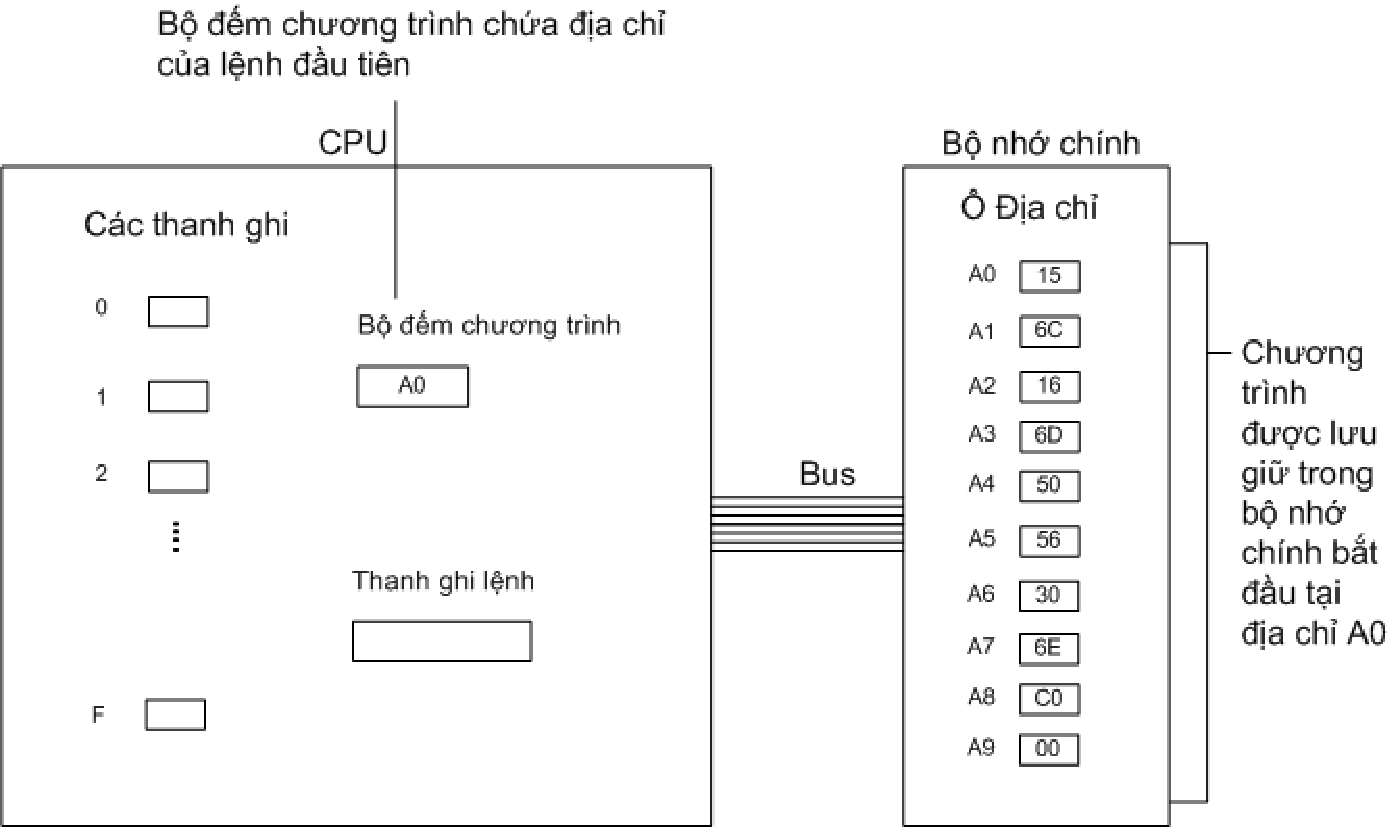
\includegraphics{ch3/fig210.pdf}}
  \caption{Chương trình từ Hình \ref{fig:fig27} được lưu giữ trong bộ nhớ để sẵn sàng thực
    hiện.}
  \label{fig:fig210}
\end{figure}


\begin{figure}
  \centering \subfloat[Lúc bắt đầu của bước nạp, lệnh bắt đầu tại địa chỉ $A0$ được nhận
  từ bộ nhớ và đặt vào thanh ghi lệnh]
  {\scalebox{0.8}{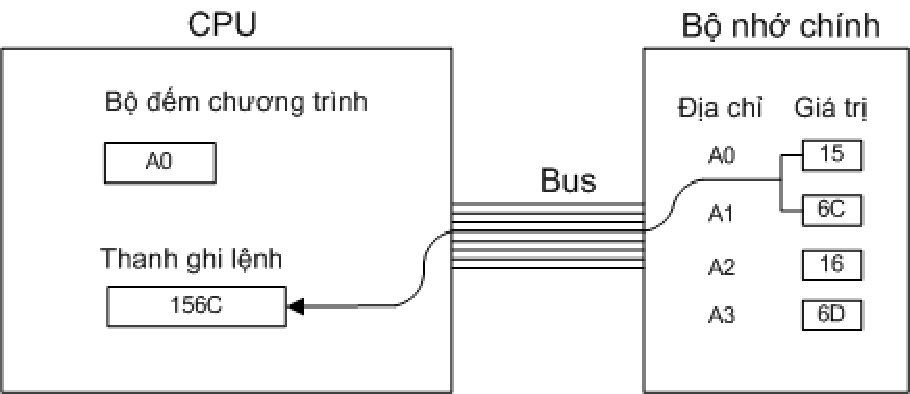
\includegraphics{ch3/fig211a.pdf}} \label{fig:fig211a}}

  \subfloat[Sau đó bộ đếm chương trình tăng lên để trỏ vào lệnh tiếp theo.]
  {\scalebox{0.8}{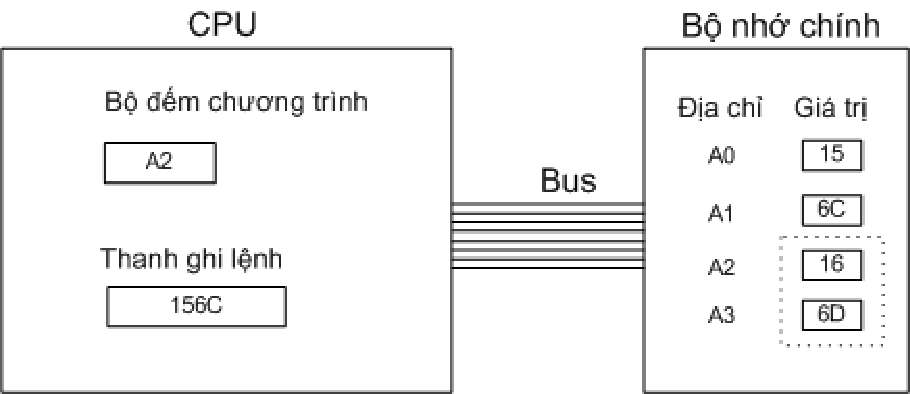
\includegraphics{ch3/fig211b.pdf}} \label{fig:fig211b}}
  \caption{Thực hiện bước nạp của chu kỳ máy.}
\end{figure}


Đơn vị điều khiển bắt đầu bước nạp của chu kỳ máy bằng cách lấy lệnh nằm trong bộ nhớ
chính tại địa chỉ $A0$ và đặt lệnh này ($156C$) trong thanh ghi lệnh (Hình
\ref{fig:fig211a}). Chú ý rằng, một lệnh trong máy của ta có độ dài $16$ bít (bằng $2$
byte). Bởi vậy nó sẽ chiếm hai ô nhớ $A0$ và $A1$ trong bộ nhớ. Đơn vị điều khiển được
thiết kế để đặt nội dung cả hai ô nhớ này vào thanh ghi lệnh (độ dài $16$ bít).  Nó tăng
bộ đếm chương trình lên hai giá trị để trỏ tới địa chỉ của lệnh tiếp theo (Hình
\ref{fig:fig211b}). Vậy, ở cuối bước nạp của chu kỳ máy đầu tiên, bộ đếm chương trình và
thanh ghi lệnh chứa dữ liệu sau đây:

\begin{itemize}
\item[] Bộ đếm chương trình: $A2$

\item[] Thanh ghi lệnh: $156C$
\end{itemize}

Sau đó, đơn vị điều khiển phân tích lệnh trong thanh ghi lệnh và kết luận rằng đây là lệnh
``nạp thanh ghi $5$ bằng nội dung của ô nhớ tại địa chỉ $6C$''.  Việc nạp được thực hiện
trong bước thực hiện của chu kỳ máy. Đơn vị điều khiển lại bắt đầu chu kỳ tiếp theo.

Chu kỳ này bắt đầu với việc nạp lệnh $166D$ từ hai ô nhớ bắt đầu tại địa chỉ $A2$. Đơn vị
điều khiển đặt lệnh này vào thanh ghi lệnh và tăng bộ đếm chương trình lên $A4$. Bây giờ
đơn vị điều khiển giải mã lệnh $166D$ và xác định rằng phải nạp thanh ghi $6$ với nội dung
của ô nhớ tại địa chỉ $6D$. Thanh ghi $6$ được nạp trong bước thực hiện của chu kỳ máy.

Bởi vì bộ đếm chương trình bây giờ chứa $A4$, đơn vị điều khiển đọc lệnh tiếp theo tại địa
chỉ này. Kết quả là $5056$ được đặt trong thanh ghi lệnh, và bộ đếm chương trình được tăng
lên thành $A6$. Đơn vị điều khiển bây giờ giải mã nội dung thanh ghi lệnh và thực hiện nó
bằng cách kích hoạt mạch cộng số bù hai với đầu vào là các thanh ghi $5$ và~$6$.

Trong bước thực hiện này, ALU thực hiện phép cộng và đặt kết quả vào thanh ghi~$0$ (theo
yêu cầu của đơn vị điều khiển), và thông báo với đơn vị điều khiển rằng nó đã kết
thúc. Đơn vị điều khiển sau đó bắt đầu chu kỳ máy khác. Một lần nữa, với sự trợ giúp của
bộ đếm chương trình, nó nạp lệnh tiếp theo ($306E$) từ hai ô nhớ bắt đầu tại địa chỉ $A6$
và tăng bộ đếm chương trình thành $A8$. Lệnh này được giải mã và thực hiện. Tại điểm này,
giá trị tổng được đặt vào ô nhớ tại vị trí $6E$.

Lệnh tiếp theo được nạp bắt đầu tại địa chỉ $A8$, và bây giờ bộ đếm chương trình được tăng
thành $AA$. Nội dung của thanh ghi lệnh là $C000$ và được giải mã là lệnh dừng chương
trình. Kết quả là, máy dừng tại bước thực hiện của chu kỳ máy, và hoàn tất việc chạy
chương trình.

Tóm lại, quá trình mà máy thực hiện lệnh cũng giống như ta đã làm để theo dõi chi
tiết từng lệnh. Nếu ta giữ vị trí bằng cách đánh dấu lệnh thì máy tính sử dụng bộ
đếm chương trình. Sau khi xác định lệnh nào tiếp theo sẽ được thực hiện, ta có thể
đọc lệnh xem ý nghĩa của nó là gì. Điều đó có nghĩa rằng ta đã thực hiện được nhiệm
vụ yêu cầu và quay trở lại danh sách để thực hiện lệnh tiếp theo giống như máy thực hiện
lệnh trong thanh ghi và quay trở lại với quá trình nạp tiếp theo.

\subsection*{Chương trình hay dữ liệu}
Nhiều chương trình có thể được lưu trữ đồng thời trong bộ nhớ chính của máy tính, miễn là
chúng ở những vị trí khác nhau. Việc xác định chương trình nào sẽ được chạy đơn thuần chỉ
là việc đặt một giá trị thích hợp cho bộ đếm chương trình.

Tuy nhiên, ta cũng phải để ý rằng, dữ liệu cũng được chứa trong bộ nhớ chính và được
mã hóa dưới dạng các dãy $0$ và $1$, máy tính không thể biết được đâu là dữ liệu và đâu là
chương trình. Nếu bộ đếm chương trình được trỏ đến một vùng dữ liệu thay vì vùng cho
chương trình, máy tính sẽ đọc các bít dữ liệu như các lệnh và thực hiện chúng. Kết quả
chạy chương trình lúc đó phụ thuộc vào dữ liệu đọc được và không thể dự đoán trước được nó
sẽ làm gì.

Ta cũng không nên kết luận rằng việc để chương trình và dữ liệu nằm chung trong bộ nhớ
chính là ý tưởng tồi. Trên thực tế, điều này rất có ích. Nó cho phép một chương trình thao
tác một chương trình khác (hoặc thậm chí với bản thân nó) giống như nó là dữ liệu. Hãy
tưởng tượng, ví dụ chương trình có khả năng học bằng cách tự thay đổi bản thân nó để phản
hồi lại các tương tác với môi trường bên ngoài. Hoặc thậm chí có tồn lại một loại chương
trình có thể viết và thực hiện một chương trình khác để giải quyết vấn đề cho trước.

\subsection*{Câu Hỏi \& Bài Tập}
\begin{enumerate}
\item Giả sử rằng các ô nhớ tại địa chỉ từ $00$ tới $05$ trong máy mô tả bởi Phụ lục
  \ref{phuluc1} chứa dãy bít (dưới dạng hexa) được cho trong bảng sau:

\begin{tabular}{cc}
  Địa chỉ & Nội dung \\
  $00$    & $14$     \\
  $01$    & $02$     \\
  $02$    & $34$     \\
  $03$    & $17$     \\
  $04$    & $C0$     \\
  $05$     & $00$
\end{tabular}

Nếu ta bắt đầu cho máy chạy với bộ đếm chương trình chưa giá trị $00$, vậy khi máy
dừng thì ô nhớ tại địa chỉ $17$ (ở dạng hexa) sẽ chứa giá trị bao nhiêu?

\item Giả sử rằng các ô nhớ từ $B0$ tới $B8$ trong máy mô tả ở Phụ lục \ref{phuluc1} chứa
  dãy bít (dưới dạng hexa) được cho bởi bảng sau:

\begin{tabular}{cc}
  Địa chỉ & Nội dung \\
  $B0$    & $13$     \\
  $B1$    & $B8$     \\
  $B2$    & $A3$     \\
  $B3$    & $02$     \\
  $B4$    & $33$     \\
  $B5$     & $B8$ \\
  $B6$    & $C0$     \\
  $B7$    & $00$     \\
  $B8$     & $0F$ 
\end{tabular}
\begin{enumerate}
\item Nếu chương trình bắt đầu tại địa chỉ $B0$, nội dung (tính theo bít) của thanh ghi số
  $3$ sau khi lệnh đầu tiên được thực hiện sẽ là bao nhiêu?

\item Nội dung của ô nhớ tại địa chỉ $B8$ là bao nhiêu sau khi lệnh kết thúc chương trình
  được thực hiện?
\end{enumerate}

\item \label{ex:233} Giả sử rằng các ô nhớ từ $A4$ tới $B1$ trong máy mô tả ở Phụ lục
  \ref{phuluc1} chứa dãy bít (dưới dạng hexa) được cho bởi bảng sau:
 
\begin{tabular}{cc}
  Địa chỉ & Nội dung \\
  $A4$    & $20$     \\
  $A5$    & $00$     \\
  $A6$    & $21$     \\
  $A7$    & $03$     \\
  $A8$    & $22$     \\
  $A9$     & $01$ \\
  $AA$    & $B1$     \\
  $AB$    & $B0$     \\
  $AC$     & $50$ \\
  $AD$    & $02$     \\
  $AE$     & $B0$ \\
  $AF$    & $AA$     \\
  $B0$    & $C0$     \\
  $B1$     & $00$ 
\end{tabular}

Hãy trả lời các câu hỏi dưới đây với giả sử rằng máy bắt đầu với bộ đếm chương trình chứa
giá trị $A4$.

\begin{enumerate}
\item Giá trị của thanh ghi $0$ bằng bao nhiêu sau khi lệnh tại địa chỉ $AA$ được thực
  hiện lần đầu tiên?

\item Giá trị của thanh ghi $0$ bằng bao nhiêu khi lệnh tại địa chỉ $AA$ được thực hiện
  lần thứ hai ?

\item Lệnh tại địa chỉ $AA$ sẽ được thực hiện bao nhiêu lần trước khi máy dừng?
\end{enumerate}

\item \label{ex:234} Giả sử rằng các ô nhớ từ $F0$ tới $F9$ trong máy mô tả ở Phụ lục
  \ref{phuluc1} chứa dãy bít (dưới dạng hexa) được cho bởi bảng sau:
 
  \begin{tabular}{cc}
    Địa chỉ & Nội dung \\
    $F0$    & $20$     \\ 
    $F1$    & $C0$     \\
    $F2$    & $31$     \\
    $F3$    & $F8$     \\
    $F4$    & $20$     \\
    $F5$     & $00$ \\
    $F6$    & $30$     \\
    $F7$    & $F9$     \\
    $F8$     & $FF$ \\
    $F9$    & $FF$     \\
  \end{tabular}

  Nếu ta cho máy bắt đầu với bộ đếm chương trình chứa $F0$, máy thực hiện nhiệm vụ
  gì khi nó đi tới lệnh tại địa chỉ $F8$?
\end{enumerate}

\section{Các lệnh số học và logic}
\label{sec:2.4}
Như đã chỉ ra ở phần trước, nhóm lệnh số học và logic bao gồm các lệnh thực hiện các phép
toán số học, logic và các phép toán dịch. Trong phần này, ta sẽ xem chi tiết các
phép toán này.

\subsection*{Các Phép Toán Logic}
Ta đã xem xét các phép toán logic $\AND$, $\OR$, $\XOR$ (tuyển loại) trong Chương
\ref{chap:1}, như các phép toán hai ngôi, có hai đầu vào và một đầu ra đều một bít. Các
phép toán này có thể mở rộng cho đầu vào, đầu ra là các dãy bít bằng cách áp dụng các phép
toán cơ bản cho các từng bít tương ứng trong dãy. Ví dụ, kết quả của việc $\AND$ hai dãy
bít $10011010$ và $11001001$ cho kết quả là
\begin{flushleft}
  \begin{tabular}{ll}
    & $10011010$ \\
    $\AND$ & $11001001$\\
    \hline
    &10001000
  \end{tabular}
\end{flushleft}
bằng việc đơn thuần áp dụng phép toán $\AND$ cho từng cặp bít tương ứng ở các cột. Cũng
tương tự, cho các phép toán $\OR$ và $\XOR$
\begin{flushleft}
  \begin{tabular}{ll}
    & $10011010$ \\
    $\OR$ & $11001001$\\
    \hline
    &11011011
  \end{tabular}
  \qquad \qquad \qquad
  \begin{tabular}{ll}
    & $10011010$ \\
    $\XOR$ & $11001001$\\
    \hline
    &01010011
  \end{tabular}
\end{flushleft}

Một trong những ứng dụng chính của phép toán $\AND$ là ẩn một phần của dãy bít không làm
ta quan tâm. Ta xem xét, ví dụ, chuyện gì xảy ra nếu byte $00001111$ là toán hạng
đầu tiên của phép toán $\AND$. Không cần biết về nội dung của toán hạng thứ hai, ta
vẫn có thể kết luận rằng bốn bít trái nhất của dãy bít kết quả sẽ là $0$. Hơn nữa, bốn bít
phía phải của kết quả sẽ sao chép phần tương ứng của toán hạng thứ hai, như được chỉ ra
trong ví dụ dưới đây:
\begin{flushleft}
  \begin{tabular}{ll}
    & $00001111$ \\
    $\AND$ & $10101010$\\
    \hline
    &$00001010$
  \end{tabular}
\end{flushleft}

Cách sử dụng phép toán $\AND$ trong trường hợp này là một ví dụ của xử lý \textbf{mặt
  nạ}. Ở đây, một phép toán, được gọi là \textbf{mặt nạ}, xác định phần của toán hạng khác
sẽ ảnh hưởng đến kết quả. Trong trường hợp của phép toán $\AND$ ở trên, mặt nạ sẽ cho kết
quả là bản sao của một phép toán, với các bít $0$ sẽ thay thế vào các vị chí không cần sao
chép.

Như vậy, đây là một phép toán có ích khi thao tác với \textbf{ánh xạ bít}, là một xâu bít
trong đó mỗi bít dùng để biểu diễn sự có mặt hay vắng mặt của một đối tượng. Một ví dụ là
các ánh xạ bít trong các ứng dụng xử lý ảnh, ở đó mỗi bít được gắn với một điểm ảnh.

Vậy thì, giả sử rằng một ô nhớ tám bít (một byte) đang được sử dụng như một ánh xạ bít, và
ta muốn biết đối tượng gắn với bít thứ ba từ cao xuống thấp có mặt hay không; chúng
ta chỉ cần $\AND$ byte này với mặt nạ $00100000$, nó sẽ cho kết quả là một byte gồm toàn
bít $0$ nếu và chỉ nếu bít thứ ba từ cao xuống thấp có giá trị là $0$. Hơn nữa, nếu ta
muốn đặt bít thứ ba từ cao xuống thấp bằng $0$ mà không muốn tác động tới các bít khác,
vậy thì ta có thể $\AND$ ánh xạ bít với mặt nạ $11011111$ và lưu trữ lại kết quả vào
ánh xạ bít ban đầu.

Trong khi phép toán $\AND$ có thể được sử dụng để sao chép một phần dãy bít bằng cách đặt
các bít $0$ vào phần không cần sao chép, thì phép toán $\OR$ có thể sử dụng để sao chép
một phần của dãy bít bằng cách đặt các giá trị $1$ vào phần không cần sao chép. Để làm
điều này, một lần nữa ta lại sử dụng một mặt nạ, nhưng lần này ta chỉ ra những
vị trí bít được sao chép với các bít $0$, còn các bít $1$ chỉ ra các phần không sao
chép. Ví dụ, khi ta $\OR$ một byte với $11110000$ sẽ cho kết quả là $1111$ trong bốn bít
cao, còn bốn bít thấp là bản sao bốn bít thấp của toán hạng kia, như dưới đây:
\begin{flushleft}
  \begin{tabular}{ll}
    & $11110000$ \\
    $\OR$ & $10101010$\\
    \hline
    &$11111010$
  \end{tabular}
\end{flushleft}
Kết quả là, trong khi mặt nạ $11011111$ có thể sử dụng với phép toán $\AND$ để đặt giá trị
$0$ vào bít thứ ba từ cao xuống thấp, thì mặt nạ $00100000$ có thể được sử dụng với phép
toán $\OR$ để đặt giá trị $1$ vào vị trí này.

Một trong những ứng dụng chính của phép toán $\XOR$ là để tính phần bù của một dãy
bít. Nếu $\XOR$ một byte tuỳ ý với mặt nạ gồm tám số $1$, thì ta sẽ được phần bù của byte
này. Ví dụ, để ý quan hệ giữa toán hạng thứ hai và kết quả trong ví dụ dưới đây:
\begin{flushleft}
  \begin{tabular}{ll}
    & $11111111$ \\
    $\XOR$ & $10101010$\\
    \hline
    &$01010101$
  \end{tabular}
\end{flushleft}

Trong ngôn ngữ máy mô tả trong Phụ lục \ref{phuluc1}, các op-code $7,8$ và $9$ được sử
dụng cho các phép toán logic $\AND$, $\OR$, và $\XOR$, tương ứng. Các phép toán này yêu
cầu đầu vào là hai thanh ghi và cho ra kết quả vào một thanh ghi. Ví dụ, lệnh $7ABC$ thực
hiện $\OR$ nội dung của thanh ghi $B$ với thanh ghi $C$ và đặt kết quả vào thanh ghi $A$.

\subsection*{Các phép toán quay  và dịch}
Các phép toán trong nhóm các phép toán quay và dịch cho phép dịch chuyển các bít bên trong
một thanh ghi. Các phép toán này được phân loại theo hướng dịch chuyển (trái hoặc phải)
hoặc là xử lý quay vòng. Ta có thể xây dựng nhiều phép toán bằng cách kết hợp các khả năng
đó lại. Ta sẽ lướt nhanh các ý tưởng liên quan.

Xét một thanh ghi tám bít (một byte), nếu ta dịch nội dung của nó sang phải một bít, ta
tưởng tượng rằng bít phải nhất sẽ bị rơi ra ngoài và một lỗ trống sẽ xuất hiện ở phía trái
nhất. Nếu bít bị rơi ra ngoài và lỗ trống là khác nhau sẽ cho ta nhiều cách dịch khác
nhau. Một cách dịch là đặt bít rơi ra ngoài phía bên phải vào lỗ trống phía bên trái; kết
quả ta có \textbf{dịch vòng}, cũng còn được gọi là \textbf{quay}. Nếu ta thực hiện phép
toán quay tám lần trên một byte, thì ta đạt được chính xâu bít ban đầu.

Một kỹ thuật khác là loại bỏ bít rơi ra và luôn đặt vào lỗ trống giá trị $0$. Thuật ngữ
\textbf{dịch logic} thường được dùng cho phép toán này. Nói chung, việc dịch trái một số
nhị phân tương đương với việc nhân nó với hai, cũng tương tự như dịch trái một số thập
phân tương đương với việc nhân nó với mười. Hơn nữa, phép chia cho hai cũng có thể được
thực hiện bằng cách dịch phải. Với ý nghĩa này, trong cả hai phép dịch, ta đều phải cẩn
thận bảo toàn bít dấu trong một số hệ thống ký hiệu (ví dụ với biểu diễn bù hai). Bởi vậy,
ta thường thấy một số kiểu dịch phải luôn bảo toàn giá trị gốc của lỗ trống để giữ bít
dấu. Các phép dịch mà bít dấu không thay đổi đôi khi được gọi là phép \textbf{dịch số
  học}.

Mặc dù các phép toán dịch và quay phong phú như vậy, ngôn ngữ máy mô tả trong phần Phụ lục
\ref{phuluc1} chỉ có phép toán quay phải, với op-code là $A$. Trong trường hợp này số hexa
đầu tiên trong trường toán hạng xác định thanh ghi được quay, phần còn lại xác định số bít
cần quay. Bởi vậy lệnh $A501$ có nghĩa rằng ``Quay nội dung thanh ghi $5$ sang phải $1$
bít''.  Cụ thể, nếu thanh ghi $5$ ban đầu có nội dung là $65$ (hexa), vậy thì nó sẽ
chứa~$B2$ sau khi lệnh được thực hiện (Hình~\ref{fig:fig212}).  Các phép dịch và quay khác
có thể tạo ra bằng cách tổ hợp các lệnh trong ngôn ngữ máy của Phụ lục \ref{phuluc1}. Ví
dụ, với một thanh ghi $8$ bít, việc dịch phải ba bít đồng nhất với việc dịch trái năm bít.

\begin{figure}[tbh]
  \centering {\scalebox{0.7}{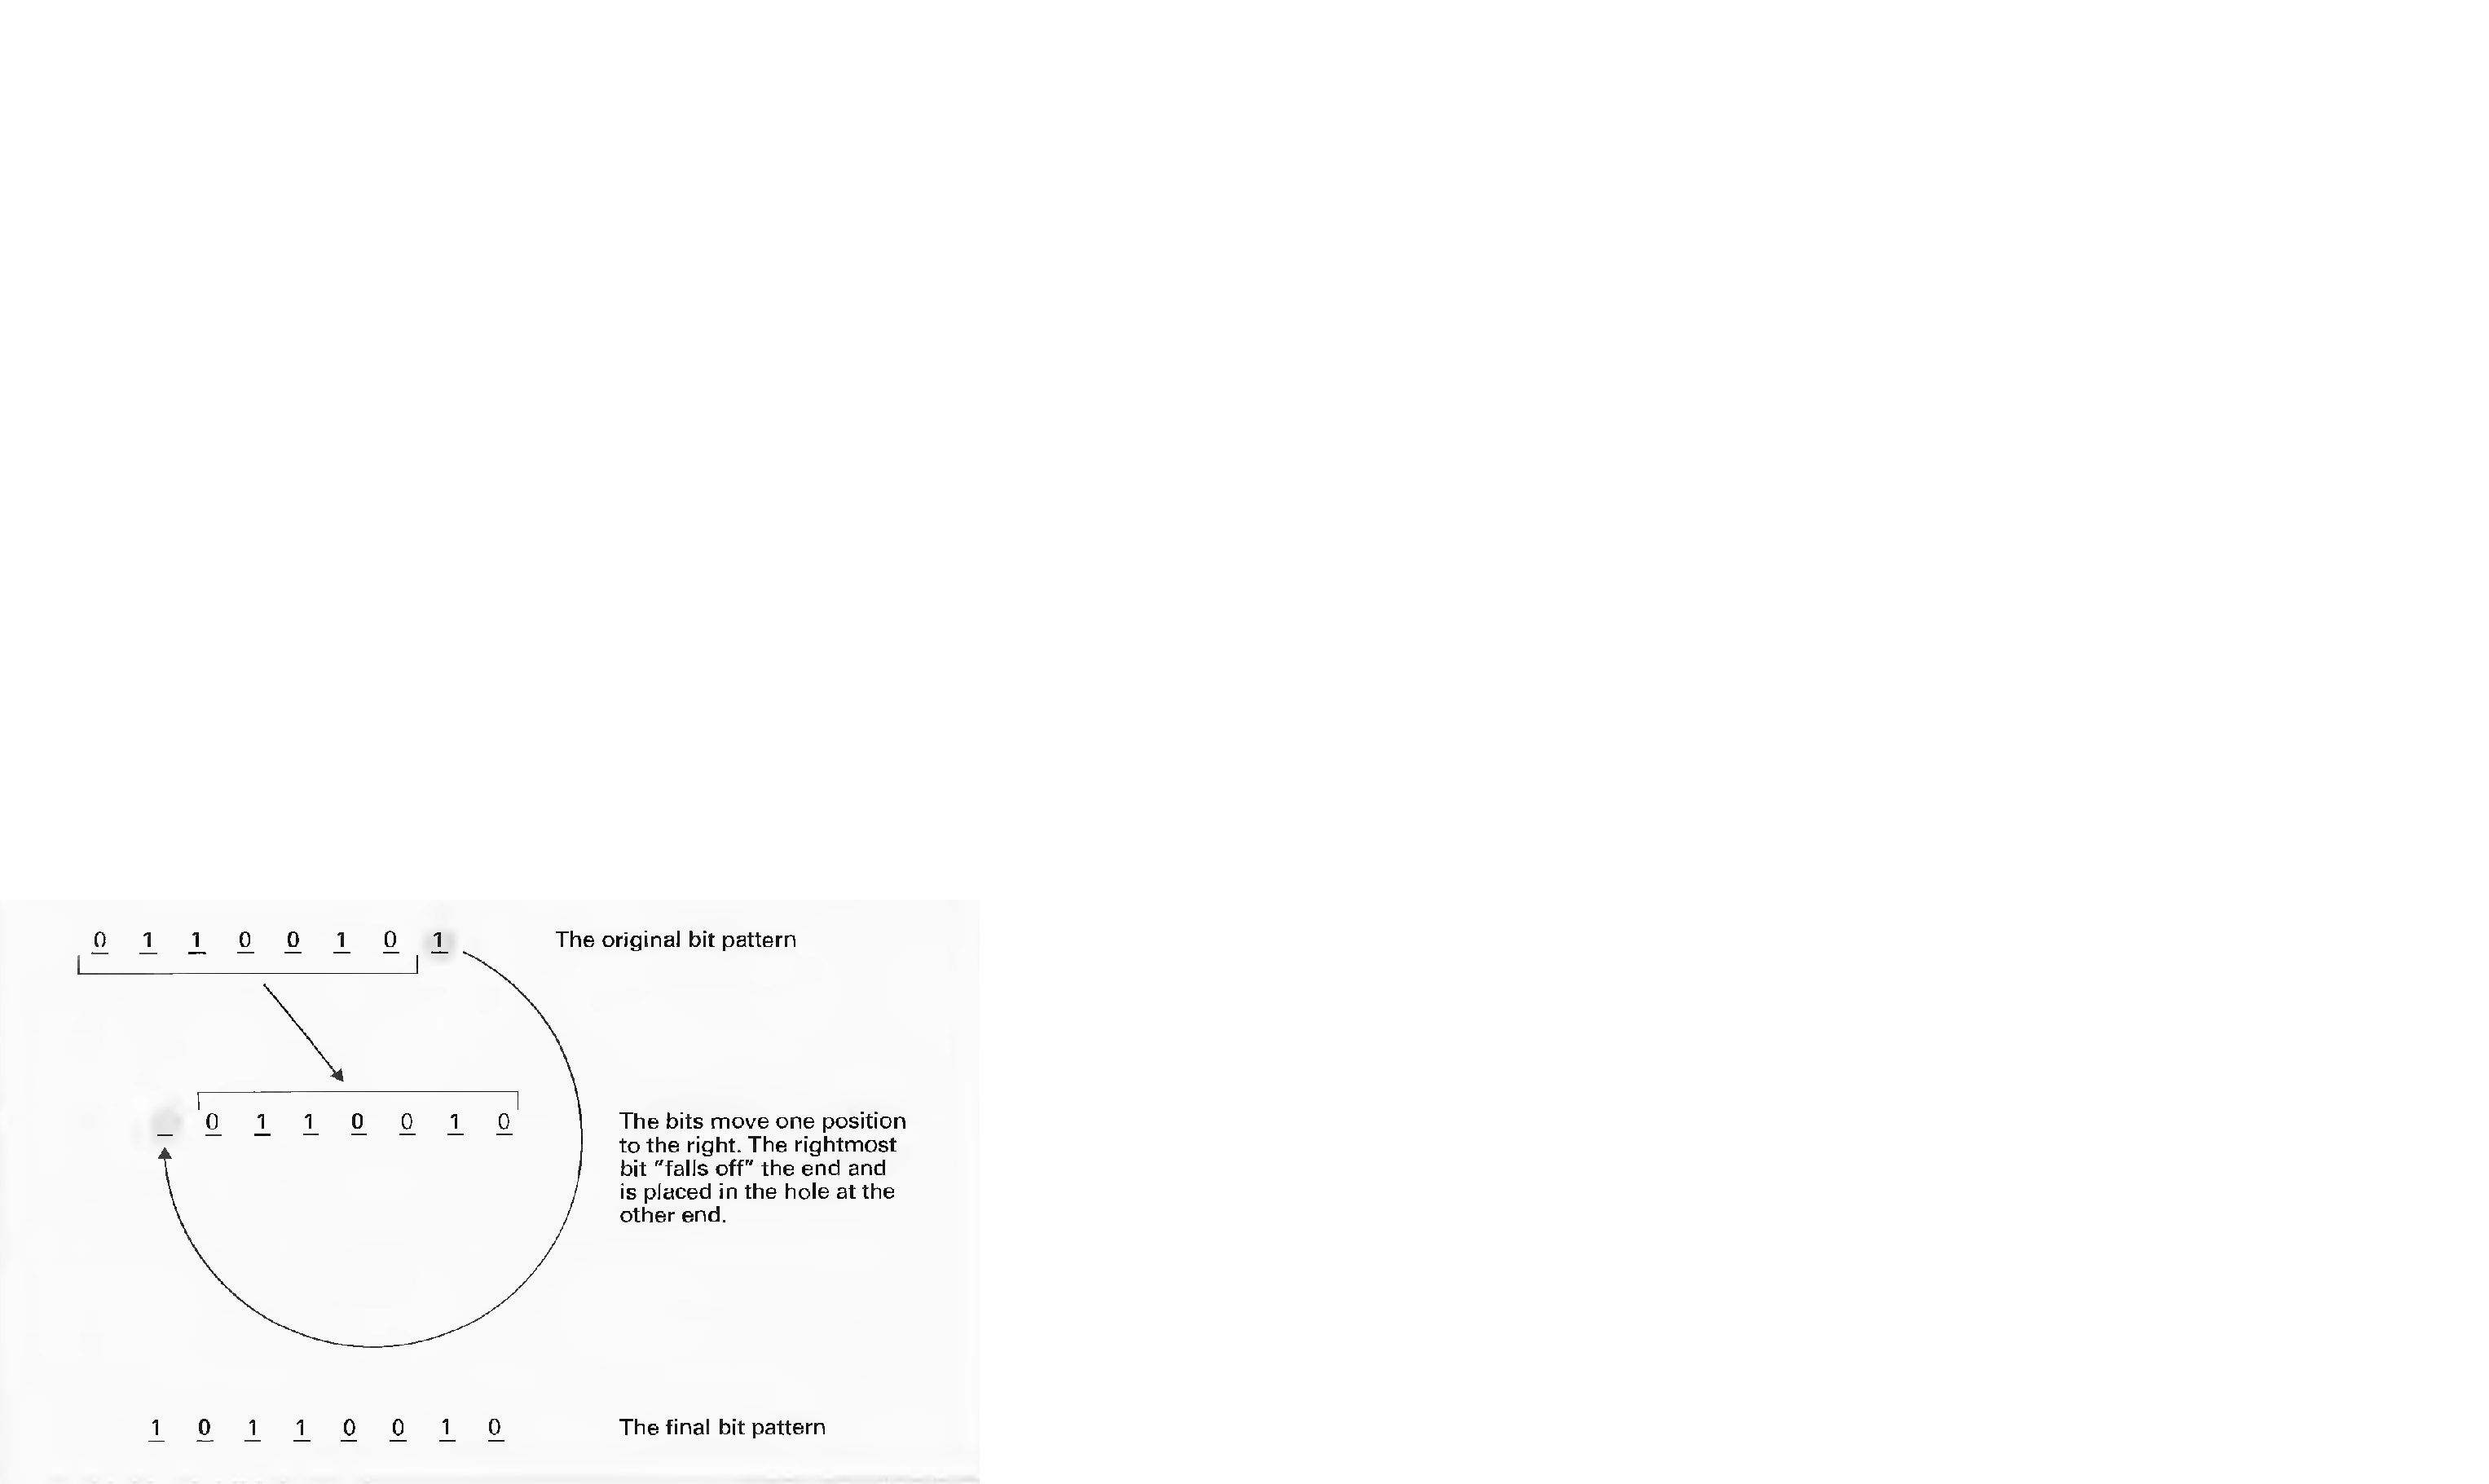
\includegraphics{ch3/fig212.pdf}} }
  \caption{Quay xâu bít $65$ ở dạng hexa sang phải một bít.}
  \label{fig:fig212}
\end{figure}

\subsection*{Các phép toán số học}

Mặc dù ta đã thảo luận về các phép toán số học cộng, trừ, nhân, và chia; nhưng ta cần chú
ý rằng giữa chúng có một vài liên hệ không rõ ràng lắm. Đầu tiên, ta đã thấy rằng phép trừ
có thể được thực hiện nhờ phép cộng và phép lấy phần bù. Hơn nữa, phép nhân chỉ đơn thuần
là lặp lại của phép cộng; và phép chia đơn thuần là lặp lại của phép trừ (ví dụ, sáu chia
cho hai bằng ba bởi vì sáu trừ cho hai chỉ được nhiều nhất là ba lần). Vì lý do này, một
vài CPU nhỏ được thiết kế chỉ có lệnh cộng hoặc chỉ có lệnh cộng hoặc trừ.

Ta để ý rằng có một vài điểm khác biệt tồn tại giữa các hệ thống số (điều này cũng
liên quan đến hai phép toán cộng có sẵn trong máy ở Phụ lục \ref{phuluc1}). Ví dụ, nếu giá
trị được cộng biểu diễn dưới dạng bù hai, quá trình cộng sẽ phải thực hiện cộng từng bít
tương ứng theo cột. Tuy nhiên, nếu các toán hạng được lưu trữ theo kiểu dấu chấm động, quá
trình cộng phải thực hiện đọc phần định trị của mỗi toán hạng, dịch chúng sang phải hoặc
trái theo phần số mũ, kiểm tra bít dấu, thực hiện phép cộng, và dịch kết quả ra theo ký
hiệu dấu phảy động. Bởi vậy, mặc dù cả hai đều là phép cộng, hoạt động của máy để thực
hiện chúng là khác nhau.

\subsection*{Câu Hỏi \& Bài Tập}
\begin{enumerate}
\item Thực hiện các phép toán sau.

  \begin{inparaenum}[a. ]
  \item \begin{tabular}{m{1cm}l}
      & $01001011$\\
      $\AND$ & $10101011$\\
      \hline
    \end{tabular} \quad
  \item \begin{tabular}{m{1cm}l}
      & $10000011$\\
      $\AND$ & $11101100$\\
      \hline
    \end{tabular} \quad
  \item \begin{tabular}{m{1cm}l}
      & $11111111$\\
      $\AND$ & $00101101$\\
      \hline
    \end{tabular}

    \bigskip

  \item \begin{tabular}{m{1cm}l}
      & $01001011$\\
      $\OR$ & $11101100$\\
      \hline
    \end{tabular} \quad 
  \item \begin{tabular}{m{1cm}l}
      & $10000011$\\
      $\OR$ & $11101100$\\
      \hline
    \end{tabular} \quad 
  \item \begin{tabular}{m{1cm}l}
      & $11111111$\\
      $\OR$ & $00101101$\\
      \hline
    \end{tabular}


    \bigskip

  \item \begin{tabular}{m{1cm}l}
      & $01001011$\\
      $\XOR$ & $11101100$\\
      \hline
    \end{tabular} \quad 
  \item \begin{tabular}{m{1cm}l}
      & $10000011$\\
      $\XOR$ & $11101100$\\
      \hline
    \end{tabular} \quad 
  \item \begin{tabular}{m{1cm}l}
      & $11111111$\\
      $\XOR$ & $00101101$\\
      \hline
    \end{tabular}
  \end{inparaenum}

\bigskip

\item Giả sử rằng bạn muốn cô lập bốn bít giữa của một byte bằng cách đặt các số~$0$ vào
  bốn bít còn lại. Vậy bạn phải sử dụng mặt nạ và phép toán gì để làm điều này?

\item Giả sử rằng bạn muốn tính phần bù của bốn bít giữa của một byte mà không muốn tác
  động vào các bít khác. Vậy bạn phải sử dụng mặt nạ gì và với phép toán gì để làm điều
  này?

\item
  \begin{enumerate}
  \item Giả sử rằng bạn thực hiện $\XOR$ hai bít đầu tiên của một xâu bít và sau đó tiếp
    tục $\XOR$ bít kết quả với bít tiếp theo, lại tiếp tục kết quả với bít tiếp
    theo... cho đến hết xâu. Kết quả cuối cùng có liên quan như thế nào đến số số $1$ xuất
    hiện trong xâu?

  \item Bài toán này có liên quan như thế nào trong việc xác định bít chẵn lẻ khi mã hoá
    thông điệp?

  \end{enumerate}

\item Thông thường, việc sử dụng các phép toán logic là thích hợp hơn so với dùng phép
  toán trên số. Ví dụ, phép toán logic $\AND$ tổ hợp hai bít giống như phép nhân. Phép
  toán logic nào gần giống như phép cộng hai số? phép toán logic bạn chỉ ra đó khác phép
  cộng trong trường hợp nào?

\item Phép toán logic cùng với mặt nạ nào có thể dùng để đổi các mã ASCII từ mã của chữ
  thường thành mã của chữ hoa? và ngược lại, từ chữ hoa thành chữ thường?

\item Kết quả thực hiện việc quay sang phải ba bít trên các xâu bít sau đây là gì?

  \begin{inparaenum}[a. ]
  \item $01101010$ \qquad \qquad \qquad
  \item $00001111$ \qquad \qquad \qquad
  \item $01111111$
  \end{inparaenum}

\item Kết quả của việc quay một bít sang trái trên các byte được biểu diễn bởi các ký hiệu
  hexa dưới đây là gì? Hãy đưa ra kết quả ở dạng hexa.

  \begin{inparaenum}[a. ]
  \item $AB$ \qquad \qquad \qquad
  \item $5C$ \qquad \qquad \qquad
  \item $B7$ \qquad \qquad \qquad
  \item $35$
  \end{inparaenum}


\item Quay một xâu tám bít sang phải ba bít thì tương đương với quay nó sang trái bao
  nhiêu bít?

\item Xâu bít nào biểu diễn tổng của $01101010$ với $11001100$ nếu chúng được biểu diễn
  dưới dạng bù hai? nếu chúng được lưu trữ dưới dạng dấu chấm động như thảo luận ở Chương
  \ref{chap:1}?

\item Sử dụng ngôn ngữ máy ở Phụ lục \ref{phuluc1}, hãy viết chương trình đặt giá trị $1$
  vào bít trái nhất của ô nhớ tại địa chỉ $A7$ mà không thay đổi các bít khác.

\item Sử dụng ngôn ngữ máy ở Phụ lục \ref{phuluc1}, hãy viết chương trình sao chép bốn bít
  giữa từ ô nhớ $E0$ vào bốn bít thấp của ô nhớ tại địa chỉ $E1$ bằng cách đặt các giá trị
  $0$ vào bốn bít cao nhất của ô nhớ tại địa chỉ $E1$.

\end{enumerate}

\section{Giao tiếp với các thiết bị khác}
\label{sec:2.5}
Bộ nhớ chính và CPU là trung tâm của máy tính. Trong phần này, ta sẽ thảo luận làm thế nào
phần trung tâm này, cái mà ta sẽ gọi là máy tính, giao tiếp với các thiết bị ngoại vi như
hệ thống lưu trữ khối, máy in, bàn phím, chuột, màn hình, camera số, và thậm chí với máy
tính khác.

\subsection*{Vai Trò của Bộ Điều Khiển}

Việc giao tiếp giữa máy tính và các thiết bị khác thông thường được thực hiện thông qua
một bộ phận trung gian gọi là \textbf{bộ điều khiển}. Trong trường hợp máy tính cá nhân,
một bộ điều khiển có thể bao gồm hệ thống mạch điện cắm vào bảng mạch chính của máy tính
hoặc, cho tính mềm dẻo, nó có thể có dạng một bảng mạch điện cắm vào khe cắm trên bảng
mạch chính. Trong cả hai trường hợp, bộ điều khiển nối bằng cáp bên trong máy tính tới các
thiết bị ngoại vi hoặc có thể tới bộ kết nối, gọi là \textbf{cổng} (port), nằm phía sau
máy tính ở đó các thiết bị bên ngoài có thể gắn với nó. Các bộ điều khiển này đôi khi bản
thân nó cũng là một máy tính nhỏ, cũng có bộ nhớ của mạch và CPU đơn giản thực hiện chương
trình điều khiển.

Bộ điều khiển dịch các thộng điệp và dữ liệu đến/đi thành dạng tương thích giữa đặc trưng
bên trong của máy tính và thiết bị ngoại vi gắn với nó. Ban đầu, mỗi bộ điều khiển được
thiết kế cho một kiểu thiết bị đặc biệt. Bởi vậy, mua thêm một thiết bị ngoại vi mới cũng
phải mua thêm bộ điều khiển mới.

Tuy nhiên gần đây, một vài giải pháp đã được đưa ra trong lĩnh vực máy tính cá nhân để
chuẩn hoá, như là \textbf{Universal Serial Bus (USB)} và \textbf{FireWire}. Theo cách này,
một bộ điều khiển có thể điều khiển rất nhiều thiết bị. Ví dụ, một bộ điều khiển USB có
thể được sử dụng để giao tiếp giữa máy tính và một tập các thiết bị tương thích USB. Danh
sách các thiết bị này trên thị trường hiện nay bao gồm chuột, máy in, máy scan, thiết bị
lưu trữ khối, và camera số.

Mỗi bộ điều khiển giao tiếp với máy tính cũng sử dụng cùng một bus kết nối mà CPU của máy
tính và bộ nhớ chính sử dụng để giao tiếp với nhau (Hình~\ref{fig:fig213}). Nó có thể theo
dõi tín hiệu đang được gửi giữa CPU và bộ nhớ cũng như đặt tín hiệu của nó vào trong bus.

\begin{figure}
  \centering \scalebox{0.5}{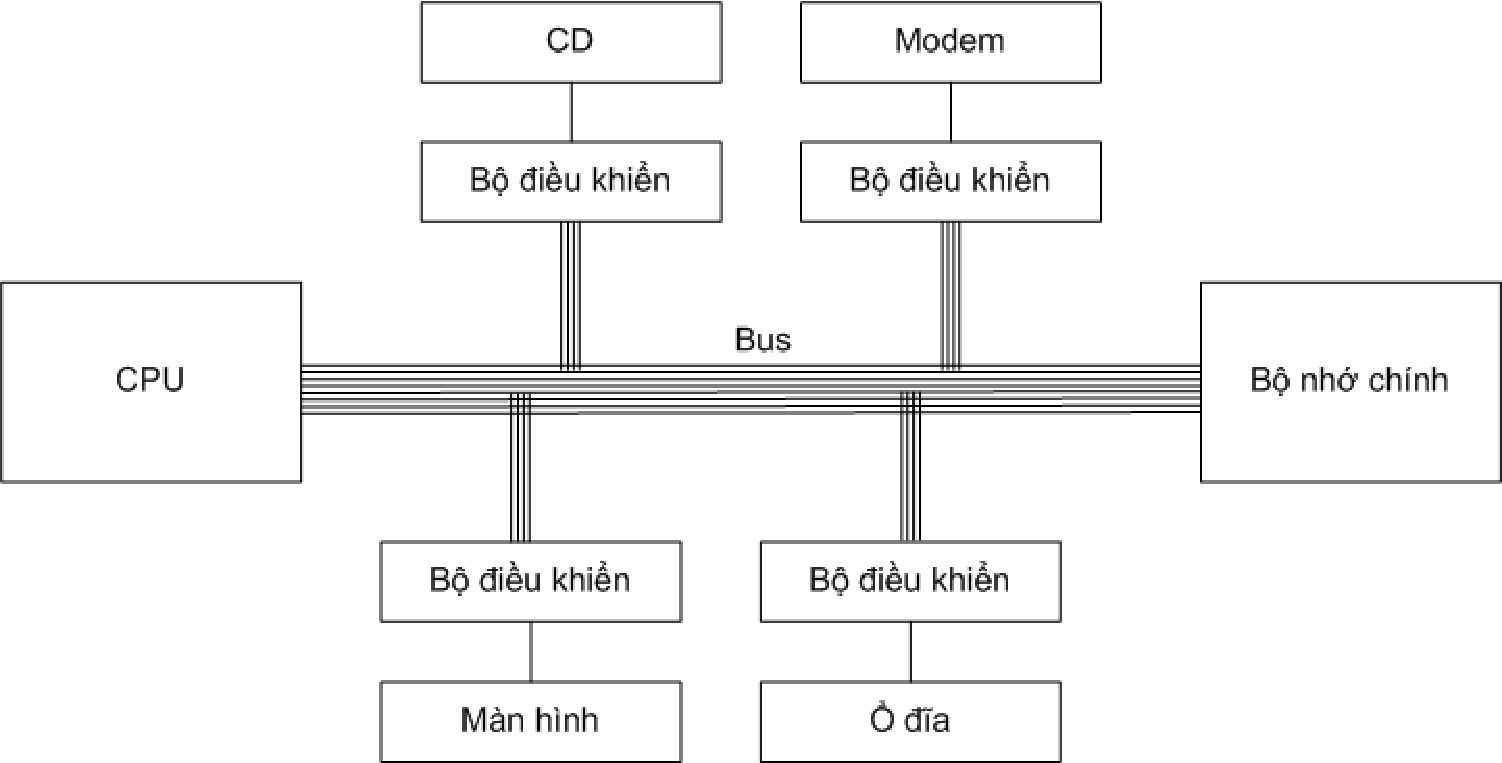
\includegraphics{ch3/fig213.pdf}}
  \caption{Bộ điều khiển gắn với một Bus của máy.}
  \label{fig:fig213}
\end{figure}

Với cách bố trí này, CPU có thể giao tiếp với các bộ điều khiển được gắn với bus giống như
nó giao tiếp với bộ nhớ chính. Để gửi một dãy bít tới bộ điều khiển, dãy bít đầu tiên phải
nằm trong thanh ghi đa năng. Và một lệnh tương tự như lệnh STORE sẽ được thực hiện bởi CPU
để ``lưu trữ'' dữ liệu vào bộ điều khiển. Để nhận một dãy bít từ bộ điều khiển, một lệnh
tương tự lệnh~LOAD sẽ được sử dụng.

Có một vài kiểu máy tính được thiết kế để chuyển dữ liệu từ/tới bộ điều khiển dùng cùng
op-code LOAD và STORE, là các lệnh giao tiếp với bộ nhớ chính. Trong các trường hợp này,
bộ xử lý được thiết kế để đáp ứng lại các ô nhớ tại các chỉ xác định gán cho các bộ điều
khiển. Trong khi đó bộ nhớ chính được thiết kế để bỏ qua các vị trí này. Bởi vậy, khi CPU
gửi thông điệp tới bus để lưu trữ một dãy bít tại các ô nhớ được gán cho bộ điều khiển,
dãy bít này thực sự được ``lưu trữ'' trong bộ điều khiển thay vì trong bộ nhớ. Tương tự,
nếu CPU cố gắng đọc dữ liệu từ một vị trí bộ nhớ như vậy bằng lệnh~LOAD, nó sẽ nhận được
dãy bít từ đơn vị điều khiển thay vì từ bộ nhớ. Cách giao tiếp này được gọi là \textbf{ánh
  xạ bộ nhớ I/O} bởi vì các thiết bị vào/ra của máy tính được ánh xạ vào trong các vùng
nhớ khác nhau (Hình~\ref{fig:fig214}).

\begin{figure}
  \centering \scalebox{0.5}{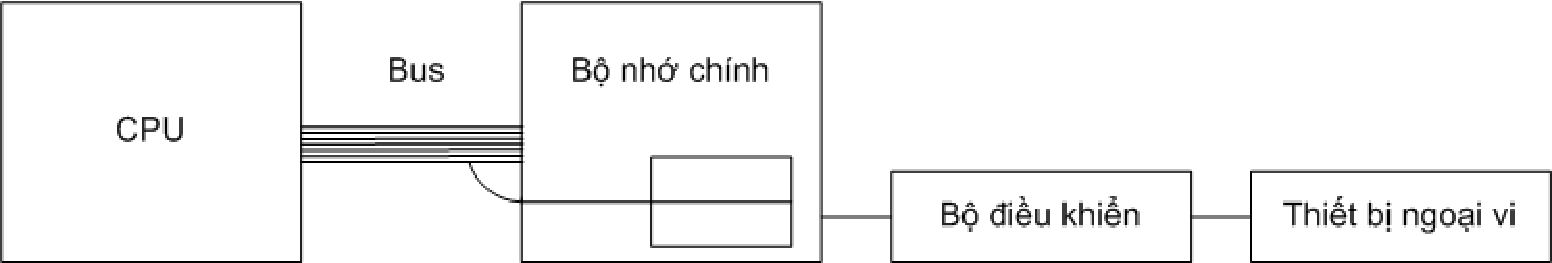
\includegraphics{ch3/fig214.pdf}}
  \caption{Biểu diễn khái niệm của ánh xạ bộ nhớ I/O.}
  \label{fig:fig214}
\end{figure}

Một lựa chọn thay thế cho ánh xạ bộ nhớ I/O là đưa ra một op-code đặc biệt ở ngôn ngữ máy
để chuyển trực tiếp tới/từ bộ điều khiển. Các lệnh với các op-code này được gọi là lệnh
I/O. Ví dụ, nếu ngôn ngữ mô tả trong Phụ lục \ref{phuluc1} theo cách tiếp cận này, nó có
thể có một lệnh kiểu như $F5A3$ với ý nghĩa rằng ``STORE nội dung của thanh ghi $5$ vào
trong bộ điều khiển xác định bởi dãy bít $A3$''.

\subsection*{Truy cập bộ nhớ trực tiếp (DMA)}
Bởi vì bộ điều khiển gắn với bus của máy tính, nó có thể thực hiện giao tiếp với bộ nhớ
chính thông qua bus (tính theo nano giây) khi CPU không sử dụng bus. Khả năng truy cập vào
bộ nhớ chính của bộ điều khiển được gọi là \textbf{truy cập bộ nhớ trực tiếp (DMA)}, và đó
là một khả năng đáng giá cho hiệu năng của máy tính. Ví dụ, để lưu trữ dữ liệu lấy từ một
sector của đĩa, CPU có thể gửi yêu cầu (được mã hoá dưới dạng một dãy bít) tới bộ điều
khiển gắn với đĩa yêu cầu đọc sector và đặt dữ liệu vào một vùng nhớ xác định của bộ
nhớ. Trong khi bộ điều khiển thực hiện thao tác đọc và gửi dữ liệu tới bộ nhớ chính qua
DMA thì CPU tiếp tục làm nhiệm vụ khác. Bởi vậy hai hoạt động sẽ được thực hiện đồng
thời. CPU vẫn thực hiện chương trình và bộ điều khiển phụ trách việc chuyển dữ liệu giữa
đĩa và bộ nhớ chính. Bằng cách này, CPU không mất thời gian liên quan đến việc chuyển dữ
liệu vốn rất chậm chạp.

Việc sử dụng DMA cũng có nhiều bất lợi do ảnh hưởng của việc truyền thông phức tạp trên
bus. Các dãy bít được chuyển giữa CPU và bộ nhớ chính, giữa CPU và các bộ điều khiển, giữa
các bộ điều khiển và bộ nhớ chính. Điều phối được tất cả những hoạt động này trên bus là
vấn đề lớn. Thậm chí với một thiết kế tốt, trung tâm của bus có thể trở thành một trở ngại
cho CPU và bộ điều khiển hoàn thành nhiệm vụ. Trở ngại này được biết như \textbf{trở ngại
  von Neumann} bởi vì nó là hệ quả của \textbf{kiến trúc von Neumann}-- CPU nạp các lệnh
của nó từ bộ nhớ vào bus trung tâm.

\subsection*{Phương pháp bắt tay (Hand Shaking)}

Chuyển dữ liệu giữa hai thành phần máy tính hiếm khi chỉ theo một chiều. Thậm chí dù ta
nghĩ rằng máy in chỉ là một thiết bị nhận dữ liệu, trên thực tế nó cũng gửi dữ liệu trở
lại máy tính. Bởi vì một máy tính có thể gửi dữ liệu tới máy in nhanh hơn rất nhiều so với
khả năng máy in có thể in chúng, nên nếu máy tính cứ nhắm mắt gửi dữ liệu, máy in sẽ bị
tụt hậu một cách nhanh chóng, và kết quả là bị mất dữ liệu. Bởi vậy một quá trình như in
dữ liệu liên quan đến hội thoại hai chiều, được biết như \textbf{bắt tay} (handshaking),
trong đó máy tính và thiết bị ngoại vi trao đổi thông tin về trạng thái thiết bị và điều
phối hoạt động của chúng.

Phương pháp bắt tay liên quan đến một \textbf{từ trạng thái} (status word), là một xâu bít
được sinh bởi thiết bị ngoại vi và gửi tới bộ điều khiển. Từ trạng thái là một \textit{ánh
  xạ bít} dùng để phản hồi lại trạng thái của thiết bị. Ví dụ, trong trường hợp của máy
in, giá trị của bít cao nhất của từ trạng thái có thể chỉ ra khi nào máy in hết giấy,
trong khi đó bít tiếp theo chỉ ra khi nào máy in sẵn sàng thêm dữ liệu. Một bít khác có
thể sử dụng để chỉ ra tình trạng kẹt giấy,... Phụ thuộc vào hệ thống, bộ điều khiển có thể
phản hồi thông tin trạng thái của nó hay nó sẵn sàng với CPU. Trong cả hai trường hợp, từ
trạng thái cho ta một cơ chế để điều phối việc giao tiếp với thiết bị ngoại vi.

\subsection*{Các phương tiện truyền thông  phổ biến}
Việc truyền thông giữa thiết bị tính toán được thực hiện trên hai kiểu truyền: song song
và tuần tự. Các thuật ngữ này chỉ ra cách mà tín hiệu được truyền. Trong trường hợp
\textbf{truyền song song}, nhiều tín hiệu được truyền cùng lúc, mỗi tín hiệu trên một
``đường'' riêng. Kỹ thuật kiểu này cho phép truyền dữ liệu nhanh chóng nhưng yêu cầu đường
truyền phức tạp. Một ví dụ kiểu này là bus bên trong máy tính, nó có nhiều dây cho phép
truyền cả khối dữ liệu và cả tín hiệu khác đồng thời. Hơn nữa, hầu hết các PC đều cho phép
ít nhất một ``cổng song song'' để qua đó dữ liệu có thể truyền cùng lúc tám bít tới/từ máy
tính.

Ngược lại, \textbf{truyền tuần tự} dựa trên việc truyền tín hiệu lần lượt, tín hiệu này
rồi mới đến tín hiệu khác, trên một đường truyền đơn. Bởi vậy, truyền tuần tự yêu cầu
đường dữ liệu đơn giản hơn so với truyền song song, đó là một lý do làm nó trở nên phổ
biến. Ví dụ về truyền tuần tự là USB và FireWire, cả hai đều liên quan đến việc truyền dữ
liệu tốc độ cao ở khoảng cách ngắn chỉ một vài mét. Với khoảng cách dài hơn (trong nhà
hoặc trong văn phòng làm việc) thì truyền tuần tự qua mạng cục bộ (Phần \ref{}), bằng dây
nối hoặc phát sóng radio, là phổ biến hơn.

Với việc truyền thông ở khoảng cách lớn hơn, thì từ nhiều năm nay đường điện thoại đã
chiếm ưu thế so với máy tính cá nhân. Đường truyền này, bao gồm một dây đơn trên đó âm
được truyền lần lượt âm này tiếp sau âm khác, vốn là hệ thống tuần tự. Việc truyền dữ liệu
số trên các đường này dẫn tới khái niệm \textbf{modem} (viết ngắn gọn cho từ điều chế-giải
điều chế, modulator-demodulator), bằng việc chuyển đổi các dãy bít thành giọng nói trên hệ
thống điện thoại, và sau đó chuyển đổi ngược từ giọng nói thành các dãy bít bằng một modem
khác ở phía đích.

Để có chất lượng cao hơn cho truyền thông khoảng cách xa, các công ty điện thoại đưa ra
một phục vụ gọi là \textbf{DSL (Digital Subscriber Line)}, ở đó sử dụng ưu điểm của các
đường điện thoại có băng tần rộng sẵn có thay vì chỉ truyền âm thanh truyền thống. Chính
xác hơn, DSL sử dụng tần số ở phía trên phạm vi của âm để truyền dữ liệu số; còn dành
đường truyền có phổ tần số thấp cho việc truyền giọng nói.  Các kỹ thuật khác cạnh tranh
với DSL bao gồm cáp, được sử dụng như hệ thống cáp tivi, và liên kết vệ tinh qua phát
radio.

\subsection*{Tốc độ truyền}
Tốc độ truyền các bít từ một thành phần của máy tính tới thành phần khác được tính bằng
\textbf{bít trên giây} (bit per second--bps). Các đơn vị chung bao gồm \textbf{Kbps}
(Kilo-bps, bằng $1$ nghìn bps), \textbf{Mbps} (mega-bps, bằng $1$ triệu bps),
\textbf{Gbps} (giga-bps, bằng $1$ tỷ bps). Chú ý phân biệt giữa bít và byte--$8$ Kbps
bằng $1$ KB trên giây. Trong viết tắt, chữ b thường được hiểu là \textit{bit} trong khi đó
chữ B hoa được hiểu là \textit{byte}.

Với các khoảng cách ngắn, USB và FireWire có tốc độ truyền hàng trăm Mbps, đủ cho các ứng
dụng đa phương tiện (multimedia). Điều này, cùng với thuận lợi về chi phí thấp, là lý do
tại sao các thiết bị này được dùng phổ biến cho việc truyền thông giữa máy tính và các
thiết bị ngoại vi cục bộ như máy in, bộ điều khiển đĩa cứng bên ngoài, các camera,...

Dù có kết hợp giữa truyền \textbf{đa công} (multiplexing), có nghĩa là mã hoá hoặc đan xen
dữ liệu sao cho một đường truyền đơn phục vụ được như nhiều đường, và kỹ thuật nén dữ
liệu, hệ thống điện thoại vẫn chỉ có thể có tốc độ khoảng $57.6$ Kbps. Nó không đủ cho các
ứng dụng đa phương tiện ngày nay. Ví dụ, để thu nhạc MP3 yêu cầu tốc độ truyền khoảng $64$
Kbps, và để có chất lượng tốt hơn cho video thì tốc độ truyền cần phải tính theo Mbps. Đó
là lý do tại sao một số lựa chọn khác như DSL, cáp, và liên kết vệ tinh, cung cấp tốc độ
truyền tốt theo phạm vi Mbps, nhanh chóng thay thế hệ thống điện thoại truyền thống cho
việc truyền dữ liệu phạm vi rộng.

Tốc độ truyền cao nhất có sẵn cho môi trường đặc biệt phụ thuộc vào kiểu của đường truyền
và công nghệ sử dụng để cài đặt của nó. Tốc độ cao nhất thường mất cân bằng so với
\textbf{băng tần} của đường truyền, mặc dù thuật ngữ \textit{băng tần} mang ý nghĩa khả
năng hơn là theo tốc độ. Có nghĩa rằng, để nói rằng đường truyền có băng tần cao (hoặc
cung cấp phục vụ \textbf{băng thông}) có nghĩa rằng đường truyền có khả năng truyền các
bít với tốc độ cao cũng như là khả năng mang một số lượng lớn thông tin đồng thời.

\subsection*{Câu Hỏi \& Bài Tập}
\begin{enumerate}
\item Giả sử rằng máy được mô tả trong Phụ lục \ref{phuluc1} sử dụng ánh xạ bộ nhớ I/O và
  tại địa chỉ $B5$ là địa chỉ cổng máy in chỉ ra dữ liệu nào sẽ được gửi để in.
  \begin{enumerate}
  \item Nếu thanh ghi $7$ chứa mã ASCII của chữ cái A, lệnh ngôn ngữ máy gì được sử dụng
    để in ký tự này ra máy in?

  \item Nếu máy thực hiện một triệu lệnh trong một giây, bao nhiêu lần ký tự này có thể
    được gửi tới máy in trong một giây?
    \label{ex2.6.1b}

  \item Nếu máy in có khả năng in năm trang văn bản trong một phút, nó sẽ có thể giữ bao
    nhiêu ký tự đang được gửi tới nó trong câu \ref{ex2.6.1b}?
  \end{enumerate}

\item Giả sử rằng ổ cứng trong máy tính cá nhân của bạn quay với tốc độ $3000$ vòng trong
  một phút, và mỗi track chứa $16$ sector, và mỗi sector chứa $1024$ byte. Hãy tính xấp xỉ
  tốc độ truyền yêu cầu giữa ổ đĩa và bộ điều khiển đĩa nếu bộ điều khiển sẽ nhận các bít
  từ ổ đĩa như là chúng được đọc từ đĩa xoay vòng?

\item Đánh giá xem mất bao lâu để truyền $300$ trang mới được mã hoá theo ASCII với tốc độ
  truyền là $57.6$ Kbps.
\end{enumerate}

\section{Các kiến trúc khác}
Trong phần này, ta sẽ xem xét một vài kiến trúc máy tính khác với kiến trúc truyền
thống đã thảo luận.
 
\subsection*{Kiến trúc đường ống (Pipelining)}

Xung điện truyền qua dây dẫn không thể nhanh hơn tốc độ ánh sáng. Bởi vì tốc độ ánh sáng
là xấp xỉ một bước chân trong một nano giây (một tỷ giây), vậy cần ít nhất $2$ nano giây
để đơn vị điều khiển trong CPU nạp một lệnh từ ô nhớ cách nó một bước chân (Lệnh yêu cầu
đọc phải được gửi tới bộ nhớ, yêu cầu ít nhất một nano giây, và lệnh phải được gửi lại đơn
vị điều khiển, yêu cầu ít nhất một nano giây nữa). Hậu quả là, để nạp và thực hiện một
lệnh trong một máy nào đó mất khoảng vài nano giây--điều này có nghĩa rằng việc tăng tốc
độ thực hiện của máy cũng không giúp nhiều cho hiệu năng của máy.

Tuy vậy, việc tăng tốc độ thực hiện không chỉ là cách duy nhất để cải thiện hiệu năng của
máy. Mục đính chính ở đây là cải thiện \textbf{năng suất} của máy, tức là số lượng công
việc mà máy có thể hoàn thành trong thời gian cho trước.

Một cách để tăng năng suất của máy mà không cần tăng tốc độ thực hiện liên quan đến khái
niệm \textbf{đường ống}. Kỹ thuật này cho phép các bước trong một chu kỳ máy có thể gối
nhau. Đặc biệt, trong khi một lệnh đang được thực hiện, lệnh tiếp theo có thể được nạp
luôn, có nghĩa rằng tại một thời điểm có thể có nhiều hơn một lệnh ở trong ``đường ống'',
và chúng ở trong các giai đoạn khác nhau của quá trình thực hiện. Vì vậy, năng suất của
máy tăng lên dù thời gian yêu cầu để nạp và thực hiện lệnh mỗi lệnh vẫn như thế. Tất
nhiên, đối với lệnh JUMP thì điều này là không hiệu quả, bởi vì trước khi nó được thực
hiện, ta vẫn chưa biết lệnh tiếp theo là lệnh gì để nạp.

Khái niệm đường ống trong thiết kế của máy tính hiện đại tiến xa hơn rất nhiều so với ví
dụ ta đã xem xét. Nó cho phép khả năng nạp một vài lệnh tại một thời điểm và thực sự thực
hiện nhiều hơn một lệnh tại một thời điểm khi lệnh này không ảnh hưởng đến lệnh khác.
   
\subsection*{Kiến trúc máy với nhiều bộ xử lý}

Xử lý đường ống có thể xem như bước đầu tiên của \textbf{xử lý song song} (có nghĩa là,
thực hiện một vài hoạt động tại một thời điểm). Mặc dù vậy, việc xử lý song song thật sự
cần nhiều hơn một đơn vị xử lý, loại máy kiểu này gọi là máy đa bộ xử lý.

Kiến trúc \textbf{MIMB} (multiple-instruction stream, multiple-data stream), có nghĩa là
nhiều luồng lệnh, nhiều luồng dữ liệu, là một kiến trúc cho việc xử lý song song. Nó thiết
kế để chứa nhiều bộ xử lý trong một máy, và các bộ xử lý này dùng chung một bộ nhớ
chính. Với cách này, máy có thể tách nhiệm vụ lớn thành nhiều nhiệm vụ nhỏ và để các bộ xử
lý thực hiện chúng một cách độc lập.  Kết quả tính toán được kết hợp lại bằng cách truyền
thông điệp qua các ô nhớ dùng chung. Rõ ràng ở đây các lệnh được xử lý song song, và mỗi
lệnh xử lý trên dữ liệu riêng của nó. Đó là lý do kiến trúc này được gọi là kiểu nhiều
luồng lệnh, nhiều luồng dữ liệu, so với kiểu kiến trúc truyền thống \textbf{SISD}, đơn
luồng lệnh, đơn luồng dữ liệu (single-instruction stream, single-data stream).

Một cách thiết kế khác là liên kết nhiều bộ xử lý lại để tất cả cùng thực hiện một dãy
lệnh, nhưng mỗi bộ xử lý lại tính toán tập dữ liệu riêng của nó. Điều này dẫn tới kiến
trúc \textbf{SIMD}, một luồng lệnh, nhiều luồng dữ liệu (single-instruction stream,
multiple-data stream).  Các máy kiểu này thích hợp cho các ứng dụng cần xử lý cùng một
nhiệm vụ nhưng trên khối dữ liệu lớn.

Một cách tiếp cận khác để xử lý song song là xây dựng máy tính lớn từ cụm các máy nhỏ hơn,
mỗi máy có bộ nhớ và CPU của riêng nó. Ở bên trong, các máy nhỏ hơn được ghép thành cặp
với các máy xung quanh nó sao cho các nhiệm vụ được gắn với toàn bộ hệ thống có thể được
chia thành các nhiệm vụ con cho các máy con. Và khi một nhiệm vụ được giao cho một máy,
nhiệm vụ này sẽ được chia thành nhiều nhiệm vụ con cho các hàng xóm của nó thực hiện đồng
thời. Kết quả là nhiệm vụ ban đầu sẽ được thực hiện ít thời gian hơn so với trên một máy
đơn.

\subsection*{Câu hỏi \& Bài tập}
\begin{enumerate}
\item Hãy xem lại Câu hỏi \ref{ex:233} của Mục~\ref{sec:2.3}, nếu máy sử dụng kỹ thuật
  đường ống đã thảo luận trong sách, trong ``đường ống'' sẽ có gì khi lệnh tại địa chỉ
  $AA$ được thực hiện?  Dưới điều kiện nào thì kỹ thuật đường ống không chứng minh được là
  có ưu điểm với lệnh này của chương trình?

\item Sẽ phải giải quyết xung đột gì khi chạy chương trình trong Câu hỏi~\ref{ex:234} của
  Mục \ref{sec:2.3} trên một máy đường ống?

\item Giả sử rằng có hai đơn vị xử lý trung tâm gắn với cùng một bộ nhớ chính phải thực
  hiện hai chương trình khác nhau. Hơn nữa, giải sử rằng một bộ xử lý cần tăng một giá trị
  ở nội dung của một ô nhớ, cũng cùng thời điểm đó, bộ xử lý khác cần thực hiện lệnh trừ
  một vào nội dung cùng ô nhớ đó. Kết quả đúng là ô nhớ đó lúc kết thúc phải có cùng giá
  trị với giá trị ban đầu.

  \begin{enumerate}
  \item Mô tả dãy hoạt động có thể làm ô nhớ kết quả lúc kết thúc có giá trị nhỏ hơn một
    so với giá trị bắt đầu.

  \item Mô tả dãy hoạt động có thể làm cho ô nhớ kết quả lúc kết thúc có giá trị lớn hơn
    một so với giá trị ban đầu.
  \end{enumerate}
\end{enumerate}
 
\section{Bài tập cuối chương}


\begin{multicols}{2}

  \begin{enumerate}
  \item
    \begin{enumerate}
    \item Các thanh ghi đa năng và các ô nhớ chính có gì giống nhau?

    \item Các thanh ghi đa năng và các ô nhớ chính có gì khác nhau?
 
    \end{enumerate}

  \item Trả lời các câu hỏi sau đây theo các mô tả của ngôn ngữ máy ở Phụ
    lục~\ref{phuluc1}.
    \begin{enumerate}
    \item Viết lệnh $2105$ (hexa) dưới dạng xâu $16$ bít.

    \item Viết op-code của lệnh $A324$ (hexa) như xâu bốn bít.

    \item Viết trường toán hạng của lệnh $A324$ (hexa) như xâu $12$ bít.
    \end{enumerate}

  \item Giả sử một khối dữ liệu được lưu trong ô nhớ của máy mô tả trong Phụ lục
    \ref{phuluc1} từ địa chỉ $B9$ tới $C1$. Có bao nhiêu ô nhớ trong khối này? Hãy liệt kê
    địa chỉ của chúng.

  \item Bộ đếm chương trình sẽ bằng bao nhiêu ngay sau khi thực hiện lệnh~$B0BA$?

  \item Giả sử rằng các ô nhớ từ địa chỉ $00$ tới địa chỉ $05$ chứa các dãy bít sau:

    \begin{tabular}{cc}
      Địa chỉ & Nội dung \\
      $00$    & $21$     \\
      $01$    & $04$     \\
      $02$    & $31$     \\
      $03$    & $00$     \\
      $04$    & $C0$     \\
      $05$     & $00$ 
    \end{tabular}

    Giả sử rằng bộ đếm chương trình khởi đầu chứa giá trị $00$, hay ghi lại chi tiết nội
    dung của bộ đếm chương trình, thanh ghi lệnh, và ô nhớ ở địa chỉ $00$ tại thời điểm
    kết thúc bước nạp trong chu kỳ máy cho đến khi máy dừng.

  \item Giả sử rằng ba giá trị $x, y$ và $z$ được lưu trữ trong bộ nhớ của máy. Mô tả dãy
    các sự kiện (nạp các thanh ghi từ bộ nhớ, lưu giữ lại giá trị trong bộ nhớ...) để có
    thể thực hiện tính toán~$x + y + z$. Tương tự, Mô tả tính toán~$(2x) +y$.

  \item Dịch các lệnh sau đây dưới dạng ngôn ngữ tự nhiên.

    \begin{inparaenum}[a. ]
    \item $407E$ \qquad
    \item $8008$ \qquad
    \item $A403$ \qquad
    \item $2835$ \qquad
    \item $B3AD$
    \end{inparaenum}

  \item Giả sử một ngôn ngữ máy được thiết kế với trường op-code bốn bít. Có bao nhiêu
    lệnh ngôn ngữ này có thể có? Có bao nhiêu lệnh có thể nếu trường op-code là tám bít?

  \item Dịch các lệnh sau đây từ ngôn ngữ tự nhiên sang ngôn ngữ máy.
    \begin{enumerate}
    \item LOAD thanh ghi số $7$ với giá trị hexa $66$.

    \item LOAD thanh ghi số $7$ với nội dung của ô nhớ $66$.

    \item $\AND$ nội dung của thanh ghi $F$ với $2$ và đặt kết quả vào thanh ghi $0$.

    \item ROTATE thanh ghi $4$ sang phải ba bít.

    \item JUMP tới lệnh tại địa chỉ $31$ nếu nội dung của thanh ghi $0$ bằng với giá trị
      trong thanh ghi~$B$.
    \end{enumerate}

  \item Viết lại chương trình trong Hình~\ref{fig:fig27} với giả sử rằng các giá trị được
    cộng và mã hóa dùng ký hiệu dấu chấm động thay vì ký hiệu bù hai.


  \item Phân loại mỗi lệnh sau đây (dạng ngôn ngữ máy trong Phụ lục~\ref{phuluc1}) theo
    các kiểu: thực hiện thay đổi nội dung của ô nhớ tại vị trí $3B$, hay lưu trữ nội dung
    của ô nhớ tại vị trí~$3B$, hay độc lập với nội dung của ô nhớ tại địa chỉ~$3B$.

    \begin{inparaenum}[a. ]
    \item $153BE$ \quad
    \item $253B$ \quad
    \item $353B$ \quad
    \item $3B3B$ \quad
    \item $403B$
    \end{inparaenum}

  \item Giả sử rằng các ô nhớ tại địa chỉ từ $00$ tới $03$ của máy được mô tả trong Phụ
    lục \ref{phuluc1} chứa dãy lệnh sau đây:

    \begin{tabular}{cc}
      Địa chỉ & Nội dung \\
      $00$    & $24$     \\
      $01$    & $05$     \\
      $02$    & $C0$     \\
      $03$    & $00$     
    \end{tabular}

    \begin{enumerate}
    \item Dịch lệnh đầu tiên ra dạng ngôn ngữ tự nhiên.

    \item Nếu máy được bắt đầu với bộ đếm chương trình chứa giá trị~$00$, khi máy dừng
      thanh ghi~$4$ sẽ chứa dãy bít gì?
    \end{enumerate}

  \item Giả sử rằng ô nhớ tại địa chỉ từ $00$ đến $02$ trong máy được mô tả trong Phụ
    lục~\ref{phuluc1} chứa các bít sau đây:

    \begin{tabular}{cc}
      Địa chỉ & Nội dung \\
      $00$    & $24$     \\
      $01$    & $1B$     \\
      $02$    & $34$     
    \end{tabular}

    \begin{enumerate}
    \item Nếu ta đặt bộ đếm chương trình bằng $00$, lệnh đầu tiên sẽ làm gì?

    \item Nếu ta đặt bộ đếm chương trình bằng $01$ thì lệnh đầu tiên sẽ làm gì ?

    \end{enumerate}

  \item Giả sử rằng ô nhớ tại địa chỉ từ~$00$ tới~$05$ trong máy mô tả trong Phụ
    lục~\ref{phuluc1} chứa các dãy bít sau đây:

    \begin{tabular}{cc}
      Địa chỉ & Nội dung \\
      $00$    & $10$     \\
      $01$    & $04$     \\
      $02$    & $30$  \\
      $03$    & $45$     \\
      $04$    & $C0$  \\
      $05$    & $00$     
    \end{tabular}

    Giả sử máy bắt đầu tại địa chỉ $00$, hãy trả lời các câu hỏi sau đây:

    \begin{enumerate}
    \item Dịch các lệnh được thực hiện sang ngôn ngữ tự nhiên.

    \item Dãy bít gì nằm trong ô nhớ tại địa chỉ $45$ khi máy dừng?

    \item Dãy bít gì nằm trong bộ đếm chương trình khi máy dừng?
    \end{enumerate}

  \item Giả sử rằng ô nhớ tại địa chỉ từ~$00$ tới~$09$ trong máy được mô tả trong Phụ lục~\ref{phuluc1} chứa dãy bít sau đây:

    \begin{tabular}{cc}
      Địa chỉ & Nội dung \\
      $00$    & $1A$     \\
      $01$    & $02$     \\
      $02$    & $2B$     \\
      $03$    & $02$     \\
      $04$    & $9C$     \\
      $05$    & $AB$     \\
      $06$    & $3C$     \\
      $07$    & $00$     \\
      $08$    & $C0$     \\
      $09$    & $00$   
    \end{tabular}

    Giả sử rằng máy bắt đầu với bộ đếm chương trình chứa $00$.

    \begin{enumerate}
    \item Giá trị nào nằm trong ô nhớ tại địa chỉ $00$ khi máy dừng?

    \item Dãy bít nào sẽ ở trong bộ đếm chương trình khi máy dừng?
    \end{enumerate}

  \item Giả sử rằng các ô nhớ tại địa chỉ từ $00$ tới $07$ trong máy mô tả trong Phụ
    lục~\ref{phuluc1} chứa nội dung sau đây:

    \begin{tabular}{cc}
      Địa chỉ & Nội dung \\
      $00$    & $1A$     \\
      $01$    & $06$     \\
      $02$    & $3A$     \\
      $03$    & $07$     \\
      $04$    & $C0$     \\
      $05$    & $00$     \\
      $06$    & $23$     \\
      $07$    & $00$
    \end{tabular}

    \begin{enumerate}
    \item Liệt kê các địa chỉ của ô nhớ chứa chương trình được thực hiện nếu ta bắt đầu
      máy với bộ đếm chương trình chứa~$00$.

    \item Liệt kê địa chỉ của các ô nhớ được sử dụng để lưu giữ dữ liệu.
    \end{enumerate}


  \item Giả sử rằng các ô nhớ tại địa chỉ từ $00$ tới $0D$ trong máy mô tả trong Phụ
    lục~\ref{phuluc1} chứa nội dung sau đây:

    \begin{tabular}{cc}
      Địa chỉ & Nội dung \\
      $00$    & $20$     \\
      $01$    & $03$     \\
      $02$    & $21$     \\
      $03$    & $01$     \\
      $04$    & $40$     \\
      $05$    & $12$     \\
      $06$    & $51$     \\
      $07$    & $12$     \\
      $08$    & $B1$     \\
      $09$    & $0C$     \\
      $0A$    & $B0$     \\
      $0B$    & $06$     \\
      $0C$    & $C0$     \\
      $0D$    & $00$    

    \end{tabular}

    Giả sử rằng máy bắt đầu với bộ đếm chương trình chứa giá trị $00$.

    \begin{enumerate}
    \item Dãy bít nào sẽ nằm trong thanh ghi $1$ khi máy dừng.

    \item Dãy bít nào sẽ nằm trong thanh ghi $0$ khi máy dừng.

    \item Dãy bít nào sẽ nằm trong bộ đếm chương trình khi máy dừng.

    \end{enumerate}


  \item Giả sử rằng các ô nhớ tại địa chỉ từ~$F0$ tới $FD$ trong máy mô tả trong Phụ lục
    \ref{phuluc1} chứa nội dung sau đây:
    \label{ex26.18}

    \begin{tabular}{cc}
      Địa chỉ & Nội dung \\
      $F0$    & $20$     \\
      $F1$    & $00$     \\
      $F2$    & $21$     \\
      $F3$    & $01$     \\
      $F4$    & $23$     \\
      $F5$    & $05$     \\
      $F6$    & $B3$     \\
      $F7$    & $FC$     \\
      $F8$    & $50$     \\
      $F9$    & $01$     \\
      $FA$    & $B0$     \\
      $FB$    & $F6$     \\
      $FC$    & $C0$     \\
      $FD$    & $00$    

    \end{tabular}

    Giả sử rằng máy bắt đầu với bộ đếm chương trình chứa giá trị $F0$, giá trị nào nằm
    trong thanh ghi $0$ khi máy thực hiện lệnh dừng tại địa chỉ $FC$.

  \item Nếu máy trong Phụ lục \ref{phuluc1} mất một micro giây (một phần nghìn giây) để
    thực hiện một lệnh, vậy nó mất bao lâu để hoàn thành chương trình trong Bài tập
    \ref{ex26.18}.

  \item Giả sử rằng các ô nhớ tại địa chỉ từ~$20$ tới~$28$ trong máy mô tả trong Phụ
    lục~\ref{phuluc1} chứa nội dung sau đây:

    \begin{tabular}{cc}
      Địa chỉ & Nội dung \\
      $20$    & $12$     \\
      $21$    & $20$     \\
      $22$    & $32$     \\
      $23$    & $30$     \\
      $24$    & $B0$     \\
      $25$    & $21$     \\
      $26$    & $20$     \\
      $27$    & $C0$     \\
      $28$    & $00$     
    \end{tabular}

    Giả sử rằng máy bắt đầu với bộ đếm chương trình chứa giá trị $20$.

    \begin{enumerate}
    \item Dãy bít nào sẽ nằm trong thanh ghi $0, 1$ khi máy dừng?

    \item Dãy bít nào sẽ nằm trong ô nhớ tại địa chỉ $30$ khi máy dừng?

    \item Dãy bít nào sẽ nằm trong ô nhớ tại địa chỉ $B0$ khi máy dừng?
    \end{enumerate}

  \item Giả sử rằng các ô nhớ tại địa chỉ từ $AF$ tới $B1$ trong máy mô tả trong Phụ lục
    \ref{phuluc1} chứa nội dung sau đây:
    \begin{center}
      \begin{tabular}{cc}
        Địa chỉ & Nội dung \\
        $AF$    & $B0$     \\
        $B0$    & $B0$     \\
        $B1$    & $AF$  
      \end{tabular}
    \end{center}
    Chuyện gì xảy ra khi ta khởi động máy với bộ đếm chương trình chứa $AF$?

  \item Giả sử rằng các ô nhớ tại địa chỉ từ $00$ tới $05$ trong máy mô tả trong Phụ lục
    \ref{phuluc1} chứa nội dung sau đây:

    \begin{tabular}{cc}
      Địa chỉ & Nội dung \\
      $00$    & $25$     \\
      $01$    & $B0$     \\
      $02$    & $35$     \\
      $03$    & $04$     \\
      $04$    & $C0$     \\
      $05$    & $00$  
    \end{tabular}

    Nếu chúng bắt đầu máy với bộ đếm chương trình chứa giá trị $00$, chuyện gì xảy ra khi
    máy dừng?

  \item Trong mỗi trường hợp dưới đây, viết một chương trình ngắn theo ngôn ngữ máy mô tả
    trong Phụ lục~\ref{phuluc1} để thực hiện các hoạt động được yêu cầu. Giả sử rằng mỗi
    chương trình của bạn được đặt trong bộ nhớ tại địa chỉ $00$.

    \begin{enumerate}
    \item Sao chép giá trị trong bộ nhớ tại vị trí $8D$ sang vị trí ô nhớ $B3$.

    \item Hoán đổi các giá trị tại địa chỉ $8D$ và $B3$.

    \item Nếu giá trị được lưu giữ trong bộ nhớ tại địa chỉ $45$ là $00$, vậy hãy đặt giá
      trị $CC$ vào địa chỉ $88$; còn trường khác, đặt giá trị~$DD$ trong bộ nhớ tại địa
      chỉ~$88$.
    \end{enumerate}

  \item Core wars - một dạng khác của trò chơi cũ xe tăng ....

  \item Viết chương trình theo ngôn ngữ máy mô tả trong Phụ lục~\ref{phuluc1} để tính tổng
    của các số bù hai được lưu giữ tại địa chỉ $A1$, $A2$, và $A4$. Chương trình của bạn
    phải lưu giữ kết quả tại địa chỉ $A5$.

  \item Giả sử rằng ô nhớ tại địa chỉ từ~$00$ tới $05$ trong máy được mô tả trong Phụ lục
    \ref{phuluc1} chứa các dãy bít sau đây (ở dạng hexa):

    \begin{tabular}{cc}
      Địa chỉ & Nội dung \\
      $00$    & $20$     \\
      $01$    & $C0$     \\
      $02$    & $30$     \\
      $03$    & $04$     \\
      $04$    & $00$     \\
      $05$    & $00$  
    \end{tabular}

    Chuyện gì xảy ra nếu ta khởi động máy với bộ đếm chương trình chứa $00$?

  \item Chuyện gì xảy ra nếu các ô nhớ tại địa chỉ~$06$ và $07$ của máy mô tả trong Phụ
    lục \ref{phuluc1} chứa dãy bít $B0$ và $B6$, tương ứng, và máy được bắt đầu với bộ đếm
    chương trình của nó chứa giá trị $06$?

  \item Giả sử rằng chương trình sau đây, được viết dưới dạng ngôn ngữ máy trong Phụ lục
    \ref{phuluc1}, được lưu giữ trong bộ nhớ bắt đầu tại địa chỉ $30$ (dạng hexa). Chương
    trình sẽ thực hiện nhiệm vụ gì?

    \begin{tabular}{l}
      $2003$ \\  
      $2101$ \\  
      $2200$ \\  
      $2310$ \\  
      $1400$ \\  
      $3410$ \\  
      $5221$ \\  
      $5331$ \\  
      $3239$ \\  
      $333B$ \\  
      $B248$ \\  
      $B038$ \\  
      $C000$
    \end{tabular}

  \item Tóm tắt các bước để máy trong Phụ lục \ref{phuluc1} thực hiện lệnh lệnh có
    op-code~$B$.

  \item Tóm tắt các bước để máy trong Phụ lục \ref{phuluc1} thực hiện lệnh lệnh có
    op-code~$5$.

  \item Tóm tắt các bước để máy trong Phụ lục \ref{phuluc1} thực hiện lệnh lệnh có
    op-code~$6$.
  
  \item Giả sử rằng thanh ghi $4, 5$ trong máy mô tả bởi Phụ lục \ref{phuluc1} chứa các
    bít $3C$ và $C8$, tương ứng. Dãy bít gì được đặt vào thanh ghi $0$ sau khi thực hiện
    mỗi lệnh sau đây:

    \begin{inparaenum}[a. ]
    \item $5045$ \qquad
    \item $6045$ \qquad
    \item $7045$ \qquad
    \item $8045$ \qquad
    \item $9045$
    \end{inparaenum}

  \item Dùng ngôn ngữ máy mô tả trong Phụ lục \ref{phuluc1}, viết chương trình thực hiệc
    các lệnh sau đây:

    \begin{enumerate}
    \item Sao chép dãy bít được lưu giữ tại địa chỉ $66$ vào vị trí tại địa chỉ $BB$.

    \item Đưa bốn bít thấp nhất của ô nhớ tại địa chỉ $34$ thành $0$ nhưng không làm thay
      đổi các bít khác.


    \item Sao chép bốn bít thấp nhất của ô nhớ tại vị trí $A5$ vào bốn bít thấp nhất của
      vị trí $A6$ nhưng không làm thay đổi các bít khác của ô nhớ $A6$.


    \item Sao chép bốn bít thấp nhất từ ô nhớ ở vị trí $A5$ vào bốn bít cao của chính nó.
      (Như thế này bốn bít đầu của ô nhớ $A5$ sẽ giống bốn bít cuối.)
    \end{enumerate}


  \item Thực hiện các phép toán sau đây:

    \begin{inparaenum}[a. ]
    \item \begin{tabular}{m{0.7cm}l}
        & $111000$\\
        $\AND$ & $101001$\\
        \hline
      \end{tabular}  

      \bigskip

    \item \begin{tabular}{m{0.7cm}l}
        & $000100$\\
        $\AND$ & $101010$\\
        \hline
      \end{tabular} 

      \bigskip

    \item \begin{tabular}{m{0.7cm}l}
        & $000100$\\
        $\AND$ & $010101$\\
        \hline
      \end{tabular}  

      \bigskip

    \item \begin{tabular}{m{0.7cm}l}
        & $111011$\\
        $\AND$ & $110101$\\
        \hline
      \end{tabular} 


      \bigskip

    \item \begin{tabular}{m{0.7cm}l}
        & $111000$\\
        $\OR$ & $101001$\\
        \hline
      \end{tabular} 
      
      \bigskip
      
    \item \begin{tabular}{m{0.7cm}l}
        & $000100$\\
        $\OR$ & $101010$\\
        \hline
      \end{tabular} 

      \bigskip

    \item \begin{tabular}{m{0.7cm}l}
        & $000100$\\
        $\OR$ & $010101$\\
        \hline
      \end{tabular}  
      
      \bigskip
      
    \item \begin{tabular}{m{0.7cm}l}
        & $111011$\\
        $\OR$ & $110101$\\
        \hline
      \end{tabular} 

      \bigskip

    \item \begin{tabular}{m{0.7cm}l}
        & $111000$\\
        $\XOR$ & $101001$\\
        \hline
      \end{tabular}  
      
      \bigskip
      
    \item \begin{tabular}{m{0.7cm}l}
        & $000100$\\
        $\XOR$ & $101010$\\
        \hline
      \end{tabular} 

      \bigskip

    \item \begin{tabular}{m{0.7cm}l}
        & $000100$\\
        $\XOR$ & $010101$\\
        \hline
      \end{tabular}   
      
      \bigskip
      
    \item \begin{tabular}{m{0.7cm}l}
        & $111011$\\
        $\XOR$ & $110101$\\
        \hline
      \end{tabular} 

    \end{inparaenum}

  \item Xác định mặt nạ và phép toán logic cần thiết để hoàn thành mục đích sau đây:
    \begin{enumerate}
    \item Đặt bốn bít ở giữa một xâu tám bít bằng $0$ mà không ảnh hưởng đến các bít khác.

    \item Lấy phần bù của một xâu tám bít.

    \item Lấy phần bù của bít cao nhất của một xâu tám bít mà không làm ảnh hưởng đến các
      bít khác.

    \item Đặt $1$ vào bít cao nhất của một xâu tám bít mà không làm ảnh hưởng đến các bít
      khác.

    \item Đặt các giá trị $1$ vào tất cả các bít \underline{trừ} bít cao nhất mà không ảnh
      hưởng đến bít cao nhất.
    \end{enumerate}

  \item Xác định phép toán logic (cùng với mặt nạ tương ứng) để khi áp dụng nó cho một xâu
    tám bít sẽ cho ta một xâu bít toàn $0$ nếu và chỉ nếu xâu đầu vào là $10000001$.

  \item Mô tả dãy các phép toán logic (cùng với các mặt nạ tương ứng) để khi áp dụng nó
    cho một xâu tám bít sẽ cho ta một xâu bít toàn $0$ nếu và chỉ nếu xâu đầu vào là xâu
    bắt đầu và kết thúc bởi $1$. Ngược lại, sẽ cho một xâu có ít nhất một bít $1$.

  \item Ta sẽ được kết quả là gì nếu quay các xâu sau đây sang trái bốn bít?

    \begin{inparaenum}[a. ]
    \item $10101$ \quad
    \item $11110000$ \quad  \\
    \item $001$ \quad
    \item $101000$ \quad
    \item $00001$
    \end{inparaenum}

  \item Ta sẽ được kết quả là gì nếu quay các xâu (ở dạng hexa) sau đây sang phải một bít?

    \begin{inparaenum}[a. ]
    \item $3F$ \quad
    \item $0D$ \quad
    \item $FF$ \quad
    \item $77$
    \end{inparaenum}

  \item
    \begin{enumerate}
    \item Lệnh nào trong ngôn ngữ ở Phụ lục \ref{phuluc1} có thể sử dụng để thực hiện quay
      thanh ghi $B$ sang phải ba bít?

    \item Lệnh nào trong ngôn ngữ ở Phụ lục \ref{phuluc1} có thể sử dụng để thực hiện quay
      thanh ghi $B$ sang trái ba bít?
    \end{enumerate}

  \item Viết chương trình ở dạng ngôn ngữ máy trong Phụ lục \ref{phuluc1} để đảo ngược nội
    dung của ô nhớ tại địa chỉ $8C$. (Có nghĩa rằng, xâu bít kết quả ở địa chỉ $8C$ khi
    đọc từ trái sang phải sẽ trùng với xâu ban đầu khi đọc từ phải qua trái.)


  \item Viết chương trình bằng ngôn ngữ máy trong Phụ lục \ref{phuluc1} để thực hiện trừ
    nội dung của ô nhớ $A1$ cho nội dung của ô nhớ $A0$ và đặt kết quả vào ô nhớ $A2$.
    Giả sử rằng các kết quả được lưu trữ dưới dạng bù hai.

  \item Một máy in, in $40$ ký tự trong một giây, có thể in kịp hay không một xâu ASCII
    (một byte cho một ký hiệu) đến một cách tuần tự với tốc độ $300$ bps? có thể với kịp
    hay không với tốc độ $1200$ bps?

  \item Giả sử rằng một người đánh máy đánh được $30$ từ trong một phút. (Một từ được xem
    như là năm ký tự.) Nếu một máy thực hiện $50$ lệnh trong một micro giây (một phần
    triệu giây), thì bao nhiêu lệnh có thể thực hiện trong khoảng thời gian giữa lúc đánh
    hai ký tự liên tiếp?

  \item Một hệ thống truyền thống có khả năng truyền các dãy tám trạng thái khác nhau với
    tốc độ cao nhất là $300$ trạng thái trong một giây. Vậy nó có thể được sử dụng để
    truyền thông tin với tốc độ bao nhiêu bít trên giây?


  \item Giả sử rằng máy trong Phụ lục \ref{phuluc1} giao tiếp với các máy in sử dụng kỹ
    thuật ánh xạ bộ nhớ I/O. Cũng giả sử rằng địa chỉ $FF$ được sử dụng để gửi ký tự tới
    máy in và địa chỉ $FE$ được sử dụng để nhận thông tin về trạng thái máy in. Đặc biệt,
    giả sử bít cao nhất tại địa chỉ $FE$ chỉ ra khi nào máy in sẵn sàng nhận một ký tự mới
    (với $0$ chỉ ra ``không sẵn sàng'' và $1$ chỉ ra ``sẵn sàng''). Bắt đầu tại địa chỉ
    $00$, viết các lệnh ở mức ngôn ngữ máy để đợi cho đến khi máy in sẵn sàng in ký tự mới
    và sau đó gửi ký tự được biểu diễn bởi xâu bít trong thanh ghi $5$ tới máy in.


  \item Viết một chương trình bằng ngôn ngữ máy mô tả trong Phụ lục \ref{phuluc1} để đặt
    các bít $0$ vào các ô nhớ từ $A0$ tới $C0$. Chương trình của bạn phải đủ nhỏ để có thể
    đặt vừa vào các ô nhớ từ $00$ tới $13$ (ở dạng hexa).


  \item Giả một máy có $20$ GB không gian lưu trữ có sẵn trên đĩa cứng; và nó nhận dữ liệu
    trên một đường kết nối điện thoại với tốc độ $14,400$ bps. Với tốc độ này, mất bao lâu
    để làm đầy không gian lưu trữ sẵn có này?


  \item Giả sử một đường truyền đang được dùng để truyền dữ liệu tuần tự với tốc độ
    $14,400$ bps. Nếu nó bị ngắt vào~$.01$ giây cuối cùng, bao nhiêu bít dữ liệu sẽ bị
    mất?

  \item Giả sử rằng bạn có $32$ bộ xử lý, mỗi cái có khả năng tính tổng của hai số có
    nhiều chữ số trong một phần triệu giây. Mô tả xem làm thế kỹ thuật xử lý song song có
    thể sử dụng để tính tổng $64$ số chỉ trong sáu phần triệu giây.

  \item Tóm tắt những khác biệt giữa hai kiến trúc RISC và CISC.

  \item Nêu hai cách tiếp cận để tăng năng lực truyền của máy tính.

  \item Mô tả xem làm thế nào việc tính trung bình của một tập hợp số sử dụng máy đa bộ xử
    lý có thể nhanh hơn so với sử dụng máy đơn bộ xử lý.

  \end{enumerate}

\end{multicols}


%%% local variables: 
%%% mode: latex
%%% TeX-master: "../tindaicuong"
%%% End: 

        

\chapter{Hệ điều hành}
\label{chap:4}

\minitoc
\vspace{0.5cm}
\noindent
Trong chương này, ta sẽ xem xét về Hệ Điều Hành, là tập các gói phần mềm để điều phối các
 hoạt động bên trong của máy cũng như để giao tiếp với thế giới bên ngoài. Cũng chính điều
hành của máy đã chuyển đổi phần cứng thành các công cụ có ích. Ta sẽ cùng tìm hiểu xem hệ
điều hành làm những gì và làm như thế nào.

\textbf{Hệ điều hành} là phần mềm điều khiển toàn bộ thao tác của máy tính. Nó cung cấp
cho người dùng cách lưu trữ và tìm kiếm các tập tin, giao diện để người dùng yêu cầu thực
hiện chương trình, và môi trường cần thiết để thực hiện các chương trình được yêu cầu.


Hệ điều hành được nhiều người biết đến nhất có lẽ là Windows, nó có nhiều phiên bản khác
nhau và được viết bởi hãng Microsoft. Một ví dụ khác là UNIX, thường được dùng cho các hệ
thống máy tính lớn cũng như cho các máy PC. Trên thực tế, Mac OS, hệ điều hành của Apple
chuyên cho dòng máy Mac, được viết dựa trên nhân của UNIX. Một ví dụ khác nữa là
GNU/Linux, dùng cho cả hệ thống lớn và nhỏ, nó gốc được phát triển bởi cộng đồng những
người say mê và không vì mục đích thương mại.  Hiện nay nó cũng được hỗ trợ bởi các công
ty lớn như IBM.

\begin{figure}
\begin{quotation}
\noindent
\textbf{Linux} \vspace{0.3cm}
\\
Nếu bạn đam mê máy tính và muốn thử nghiệm với các thành phần bên trong của một hệ điều
hành, vậy thì Linux là dành cho bạn. Linux là một hệ điều hành được thiết kế đầu tiên bởi
Linus~Torvald khi anh là sinh viên tại Trường Đại học Helsinki. Đây không phải là một sản
phẩm thuộc quyền sở hữu của ai cả và luôn có sẵn, cùng với mã nguồn và tài liệu, cũng
không có ai chịu trách nhiệm. Bởi vì nó luôn có sẵn ở dạng mã nguồn, nên nó đã trở nên phổ
biến trong giới những người say mê máy tính, các sinh viên học hệ điều hành, và những
người lập trình. Hơn nữa, Linux được thừa nhận là một trong những hệ điều hành mềm dẻo
nhất sẵn có ngày nay. Vì lý do này, nhiều công ty hiện nay đã đóng gói và đưa ra thị
trường nhiều phiên bản Linux ở dạng dễ sử dụng, và các sản phẩm này hiện nay đang cạnh
tranh với các hệ điều hành thương mại khác đã có mặt từ lâu trên thị trường. Bạn có thể
tham khảo thêm thông tin về Linux tại trang web \url{http://www.linux.org}.
\end{quotation}
\end{figure}
 

\section{Lịch sử  các hệ điều hành}
\label{sec:31}

Máy tính trong những năm $1940$ và $1950$ rất không mềm dẻo và hiệu quả. Chúng chiếm hết
cả căn phòng, và việc thực hiện chương trình yêu cầu chuẩn bị nhiều thứ: lắp các băng từ,
đặt các bìa đục lỗ vào ổ đọc, bố trí các chuyển mạch,... Việc thực hiện chương trình (ở
đây ta gọi là \textbf{công việc} (job)) được xử lý như một hoạt động riêng biệt, và máy đã
phải đã được chuẩn bị sẵn sàng từ trước để thực hiện chương trình này.  Khi chương trình
thực hiện xong, nếu ta muốn thực hiện tiếp chương trình khác thì ta lại phải lưu trữ trước
mọi băng, thẻ đục lỗ,... Khi có nhiều người muốn chia sẻ một máy, họ phải đăng ký trước
thời gian dùng máy. Trong khoảng thời gian được cấp phép, máy hoàn toàn thuộc quyền điều
khiển của người dùng. Phiên làm việc bao gồm cài đặt chương trình (mất rất nhiều thời
gian) và chạy chương trình (trong khoảng thời gian rất ngắn). Mọi thứ luôn phải làm vội
vàng vì luôn có người đang kiên nhẫn chờ để dành máy.

Trong môi trường như vậy, các hệ điều hành ban đầu chỉ nhằm đơn giản hoá việc cài đặt
chương trình và hợp lý hoá việc chuyển đổi giữa các công việc. Những cải tiến đầu tiên là
tách riêng người sử dụng và thiết bị nhằm tránh việc có quá nhiều người ra vào phòng máy
tính. Với mục đích này, các phòng máy luôn có người trực máy. Khi người dùng muốn thực
hiện một chương trình, anh ta phải gửi chương trình, dữ liệu cần chạy, và các chỉ dẫn cụ
thể về chương trình cho người trực máy, và đợi để nhận lại kết quả chạy. Về phía người
trực máy, anh ta phải bật máy, đưa các thông tin này vào thiết bị lưu trữ khối của máy nơi
một chương trình được gọi là hệ điều hành có thể đọc và thực hiện chúng. Đây là bắt đầu
của \textbf{xử lý theo lô}--các công việc cần thực hiện được tập hợp lại và thực hiện mà
không cần tương tác với người sử dụng.


Trong các hệ thống xử lý theo lô, các công việc đợi thực hiện nằm trong một thiết bị lưu
trữ khối. Thiết bị này được gọi là \textbf{hàng đợi công việc} (job queue) (Hình
\ref{fig:fig3.1}). Một \textbf{hàng đợi} là một tập các đối tượng (trong trường hợp này là
các công việc) được tổ chức theo kiểu \textbf{vào trước, ra trước} (gọi tắt là FIFO). Có
nghĩa rằng, các đối tượng được lấy ra khỏi hàng đợi theo thứ tự chúng được đưa vào. Trên
thực tế, hầu hết các hàng đợi không tổ chức chặt chẽ theo cấu trúc FIFO mà xem xét theo độ
ưu tiên của từng đối tượng. Các hệ điều hành nói chung đều cho phép xem xét các công việc
theo độ ưu tiên. Bởi vậy, một công việc nằm trong hàng đợi dù sắp đến lượt vẫn có thể bị
đẩy về sau bởi một công việc khác có độ ưu tiên cao hơn.

\begin{figure}[bt]
\centering
    \scalebox{0.35}{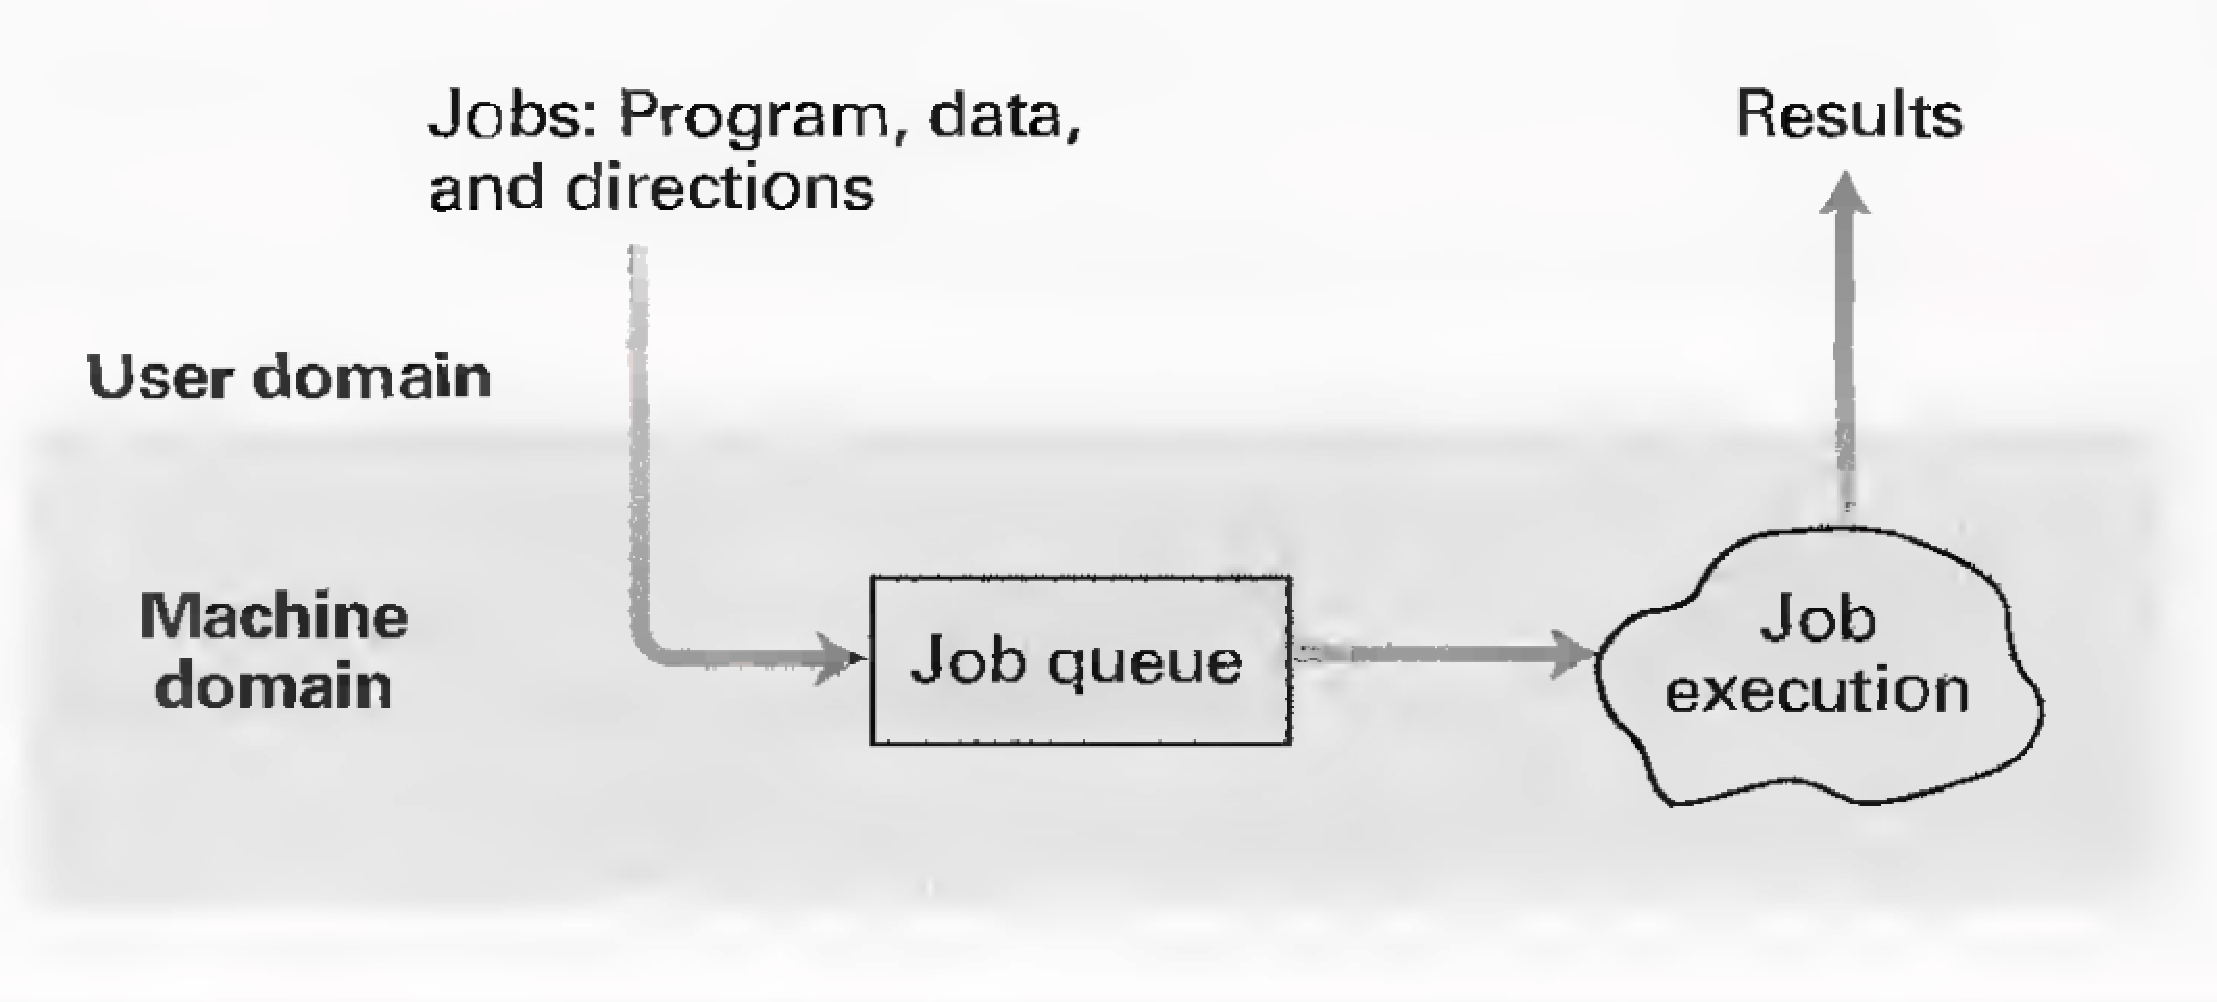
\includegraphics{ch4/fig31.pdf}}
\caption{Xử lý theo lô}
  \label{fig:fig3.1}
\end{figure}

Trong các hệ thống xử lý theo lô trước đây, mỗi công việc đi kèm với bởi một tập các chỉ
thị giải thích các bước yêu cầu người trực máy chuẩn bị theo đặc thù của công việc đó. Các
chỉ thị này được mã hoá, dùng một hệ thống gọi là ngôn ngữ điều khiển công việc (JCL). Tập
chỉ thị này được lưu trữ cùng với công việc trong hàng đợi công việc. Khi một công việc
được chọn để thực hiện, hệ điều hành in các chỉ thị này ra máy in để người trực máy tính
có thể đọc và làm theo. Ngày nay, ta vẫn thấy cách giao tiếp này, ví dụ như các báo lỗi
của hệ điều hành: ``no dial tone'', ``ổ đĩa không truy cập được'' hay ``máy in không trả
lời''.

Một trở ngại trong việc sử dụng người trực máy làm trung gian là người dùng phải gửi công
việc cho người trực máy, và do đó họ không thể tương tác được với công việc của họ. Cách
tiếp cận này có thể phù hợp với một số kiểu ứng dụng, ví dụ như xử lý bảng lương ở đó tất
cả mọi dữ liệu và cách xử lý đã được xác định trước. Tuy nhiên, trong nhiều trường hợp
cách này là không chấp nhận được, ví dụ như trong hệ thống đặt vé ở đó việc đặt và huỷ vé
phải được báo cáo ngay khi chúng xuất hiện, trong hệ thống xử lý văn bản ở đó tài liệu
được viết và viết lại liên tục, hay trong các trò chơi máy tính ở đó người dùng luôn phải
tương tác với máy.

Để thích nghi với các nhu cầu này, người ta đã phát triển các hệ điều hành mới cho phép
các chương trình thực hiện giao tiếp với người sử dụng qua trạm cuối ở xa--đặc điểm này
được gọi là \textbf{xử lý tương tác} (Hình \ref{fig:fig3.2}). Vào thời kỳ đó, các thiết bị
đầu cuối (cũng được gọi là máy trạm) chỉ có tính năng giống máy chữ--người dùng nhập dữ
liệu và đọc câu trả lời đã được máy tính in trên giấy.

\begin{figure}[tb]
  \centering \scalebox{0.35}{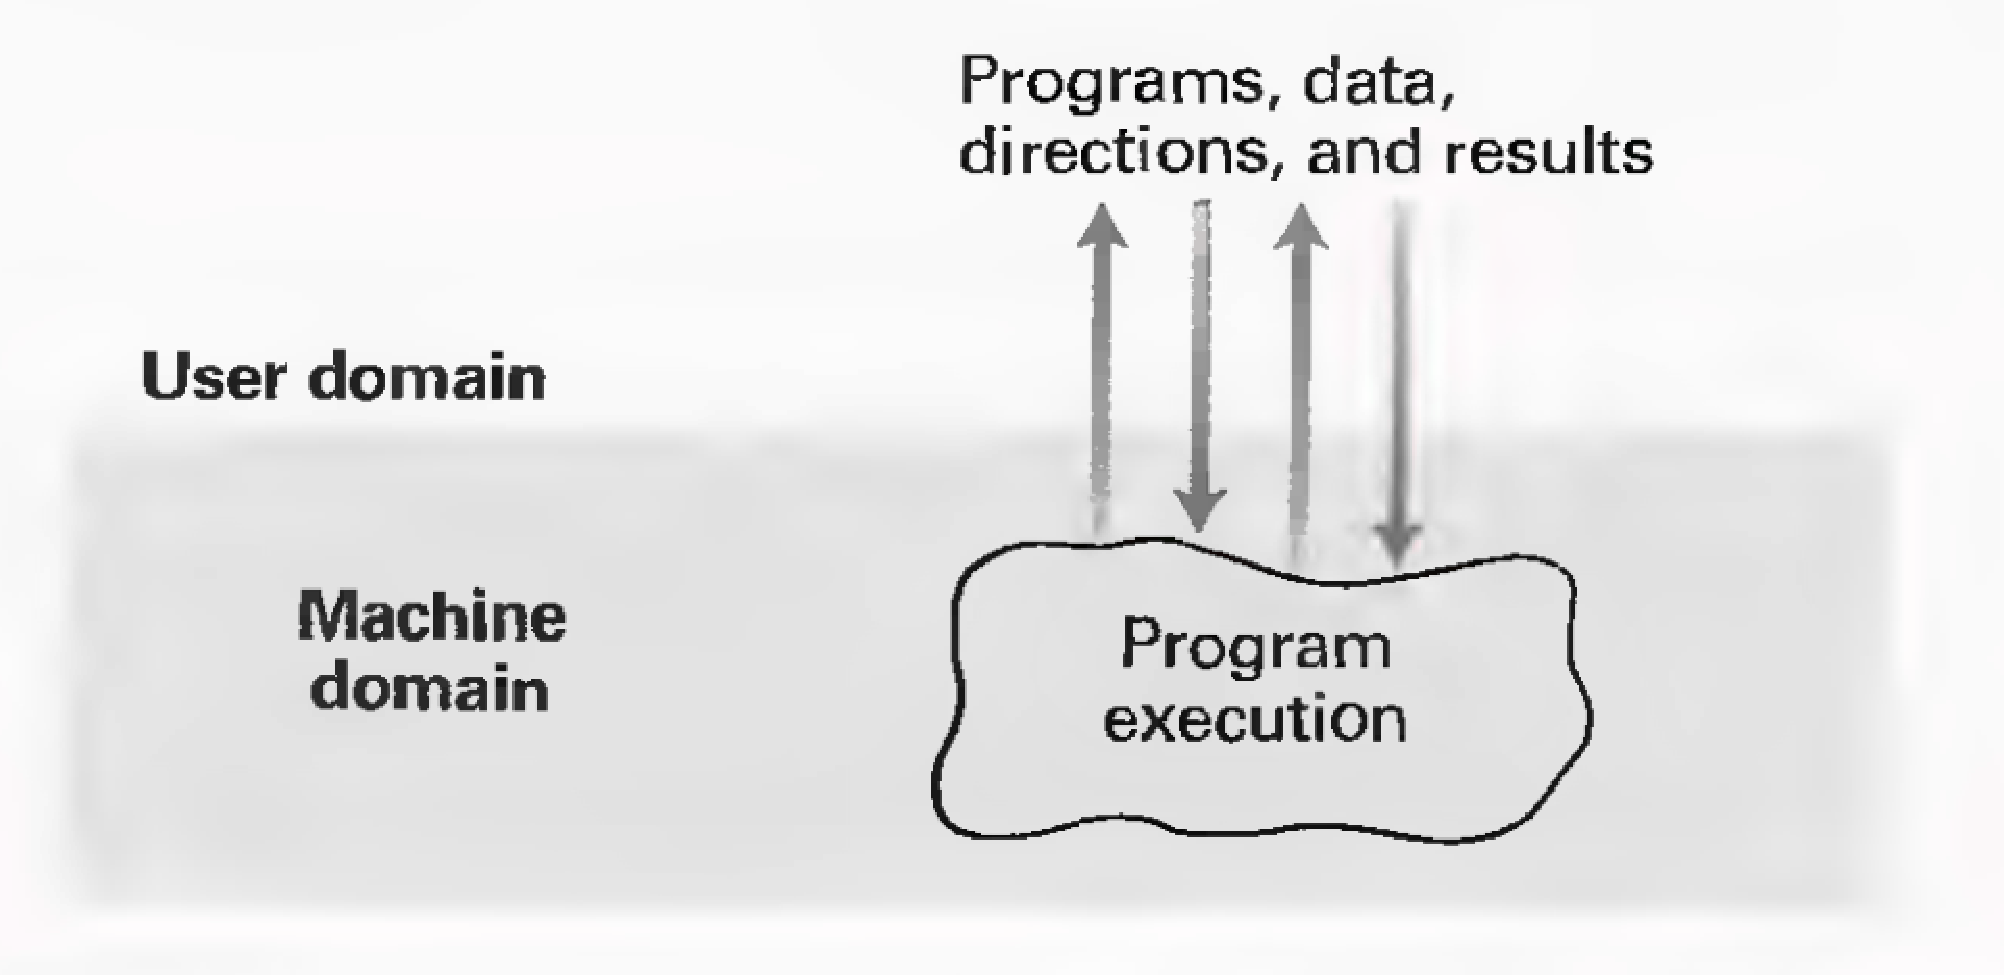
\includegraphics{ch4/fig32.pdf}}
\caption{Xử lý tương tác}
  \label{fig:fig3.2}
\end{figure}

Để việc xử lý tương tác thành công, điều hết sức quan trọng là các hoạt động của máy tính
phải đủ nhanh để phối hợp với các thao tác của người dùng thay vì ép người dùng phải chờ
đợi (ta có thể chờ đợi các các nhiệm vụ xử lý tiền lương thực hiện, nhưng không thể chấp
nhận nếu trong ứng dụng xử lý văn bản, máy tính không trả lời dấu nhắc lệnh khi các ký tự
được đánh). Các phục vụ của máy tính thoả mãn yêu cầu về thời gian được gọi là \textbf{xử
  lý thời gian thực}. Có nghĩa rằng, máy tính thực hiện nhiệm vụ đủ nhanh để để có thể
theo kịp các hoạt động của môi trường bên ngoài (thế giới thực).

Nếu hệ thống tương tác chỉ phục vụ một người dùng tại một thời điểm, vậy nó không gặp vấn
đề gì trong xử lý thời gian thực. Nhưng các máy tính trong những năm $1960$ và~$1970$ rất
đắt tiền, bởi vậy tại mỗi thời điểm, mỗi máy phải phục vụ rất nhiều người dùng. Họ làm
việc qua thiết bị đầu cuối ở xa để chuyển các phục vụ tương tác với máy, và vấn đề thời
gian thực trở thành một trở ngại. Nếu hệ điều hành cứ nhất định thực hiện một nhiệm vụ tại
một thời điểm, vậy thì chỉ một người dùng có thể thoả mãn phục vụ thời gian thực.

Một giải pháp cho vấn đề này là thiết kế hệ điều hành sao cho nó có thể chuyển việc thực
hiện các công việc khác nhau theo một chiến lược gọi là \textbf{chia sẻ thời gian thực},
đó là kỹ thuật chia thời gian thành các khoảng và sau đó hạn chế việc thực hiện mỗi công
việc trong một khoảng thời gian nhất định tại một thời điểm. Khi kết thúc mỗi khoảng, công
việc hiện hành bị đặt tạm ra bên ngoài và cho phép công việc khác tiếp tục thực hiện trong
khoảng tiếp theo. Bằng cách tráo đổi các công việc trước và sau một cách nhanh chóng theo
cách này, nó tạo ra cảm giác có nhiều công việc được chạy đồng thời. Phụ thuộc vào kiểu
công việc đang thực hiện, các hệ thống chia sẻ thời gian thực trước đây đã có thể cho phép
xử lý thời gian thực chấp nhận được với khoảng $30$ người sử dụng đồng thời. Ngày nay,
chia sẻ thời gian thực được sử dụng với hệ thống đơn người dùng cũng tốt như đa người
dùng, mặc dù về hình thức nó được gọi là \textbf{đa nhiệm}, để chỉ các hệ thống cho phép
(về mặt cảm giác) tại một thời điểm có thể có nhiều nhiệm vụ được thực hiện đồng thời.

Với sự phát triển của hệ điều hành đa người dùng và chia sẻ thời gian thực, một máy tính
đã được cấu hình như máy trung tâm kết nối với nhiều máy trạm. Từ các máy trạm này, người
dùng có thể giao tiếp trực tiếp với máy tính bên ngoài phòng máy thay vì phải gửi yêu cầu
tới người trực máy. Các chương trình sử dụng chung được lưu trữ trước trong thiết bị lưu
trữ khối của máy và hệ điều hành đã được thiết kế để thực hiện các chương trình này theo
yêu cầu từ các máy trạm. Vai trò người trực máy dần bị phai nhoà.

Ngày nay, về cơ bản không còn người trực máy nữa, đặc biệt trong lĩnh vực máy tính cá nhân
ở đó người sử dụng chịu mọi trách nhiệm thay người trực máy. Thậm chí hầu hết các máy tính
lớn không còn cần có người quản lý. Giờ đây công việc của người trực máy đã được thay bằng
người quản trị hệ thống, người chịu trách nhiệm quản lý hệ thống máy tính--có nhiệm vụ
theo dõi và thực hiện cài đặt thiết bị mới và phần mềm, bắt người dùng tôn trọng các quy
định như tạo tài khoản mới và thiết lập giới hạn không gian lưu trữ khối cho nhiều người
dùng, và cố gắng điều phối để giải quyết vấn đề gây ra trong hệ thống--hơn là thao tác với
máy trực tiếp bằng tay.

Tóm là, hệ điều hành đã phát triển từ một chương trình chỉ thực hiện nhiệm vụ đơn giản là
lưu trữ và thực hiện chương trình thành một hệ thống phức tạp điều phối việc chia sẻ thời
gian, bảo trì chương trình và các file dữ liệu trong các thiết bị lưu trữ khối của máy, và
trả lời trực tiếp yêu cầu từ người dùng.
 
Nhưng sự phát triển của các hệ điều hành vẫn chưa dừng ở đó. Sự phát triển của máy đa bộ
xử lý đã dẫn tới các hệ điều hành thực hiện đa nhiệm bằng cách gán các nhiệm vụ khác nhau
cho các bộ xử lý khác nhau thay vì chia sẻ thời gian của một bộ xử lý. Các hệ điều hành
này phải vật lộn với các vấn đề như \textbf{cân bằng tải} (các nhiệm vụ được gán một cách
động tới các bộ xử lý khác nhau sao cho mọi bộ xử lý được sử dụng một cách hiệu quả) cũng
như \textbf{scaling} (chia các nhiệm vụ thành các nhiệm vụ con tương thích với số bộ xử lý
có sẵn). Hơn nữa, sự phát triển của các mạng máy tính với nhiều máy ở khoảng cách xa được
kết nối với nhau đã dẫn tới tính cần thiết của phần mềm hệ thống để điều phối các hoạt
động của mạng. Bởi vậy lĩnh vực mạng (ta sẽ nghiên cứu chi tiết ở Chương \ref{} ) là một
trong nhiều chủ đề mở rộng của các hệ điều hành--mục đích là phát triển một hệ điều hành
đơn cho mạng rộng thay vì một mạng gồm nhiều hệ điều hành riêng lẻ.

\subsection*{Câu hỏi \& Bài tập}
\begin{enumerate}
\item Cho các ví dụ về hàng đợi. Trong mỗi trường hợp, chỉ ra tình
  huống vi phạm với cấu trúc FIFO.

\item Các hoạt động nào dưới đây yêu cầu xử lý thời gian thực?
  \begin{enumerate}
  \item In các nhãn thư điện tử

  \item Chơi một trò chơi trên máy tính

  \item Hiện các ký tự ra màn hình như chúng được nhập vào từ bàn phím

  \item Thực hiện chương trình dự báo tình trạng nền kinh tế trong năm
    tới
  \end{enumerate}

\item Nêu sự khác nhau giữa hệ điều hành xử lý thời gian thực và hệ
  điều hành tương tác?

\item Nêu sự khác nhau giữa hệ điều hành chia sẻ thời gian và đa nhiệm?
\end{enumerate}







%%% Local Variables: 
%%% mode: latex
%%% TeX-master: "../tindaicuong"
%%% End: 

\section{Kiến trúc hệ điều hành}

Để hiểu cấu tạo của một hệ điều hành, đầu tiên ta sẽ xem xét các phần mềm tìm thấy
bên trong một hệ thống máy tính. Sau đó ta sẽ trọng tâm trên bản thân hệ điều hành.

\subsection*{Tổng quan về phần mềm}

Ta sẽ tiến hành phân loại phần mềm để có cái nhìn tổng quan về phần mềm.  Lược đồ
phân loại phần mềm như vậy cũng giống như cách mà người ta phân múi giờ để mọi người đặt
đồng hồ chung chứ không có ý nghĩa phân biệt giữa sự xuất hiện của bình minh và hoàng
hôn. Hơn nữa, trong trường hợp phân loại phần mềm, tính động của phần mềm và thiếu định
nghĩa chính xác dẫn tới các thuật ngữ mâu thuẫn. Ví dụ, người sử dụng hệ điều hành Windows
của Microsoft sẽ tìm thấy nhóm phần mềm ``Accessories'' và ``Administrative Tool'' gồm
những phần mềm nằm trong cả phần ứng dụng và lớp công cụ. Cách phân loại dưới đây được
nhìn theo nghĩa kinh nghiệm về tính mở rộng và tính động của chủ đề hơn là một phát biểu
được chấp nhận rộng rãi trong thực tế.

Ta bắt đầu bằng cách chia phần mềm máy tính thành hai phạm trù rộng: \textbf{phần mềm ứng
  dụng} và \textbf{phần mềm hệ thống} (xem Hình~\ref{fig:fig3.3}). Phần mềm ứng dụng bao
gồm các chương trình nhằm thực hiện các nhiệm vụ đặc biệt. Một máy tính được dùng để bảo
quản việc kiểm kê hàng hoá tồn kho của một nhà sản xuất sẽ có các phần mềm ứng dụng khác
với một máy tính được dùng bởi một kỹ sư điện tử. Các ví dụ phần mềm ứng dụng bao gồm:
bảng tính, hệ quản trị cơ sở dữ liệu, hệ thống xuất bản desktop, hệ thống kế toán, phần
mềm phát triển chương trình, và các trò chơi.

\begin{figure}[tb]
  \centering \scalebox{0.4}{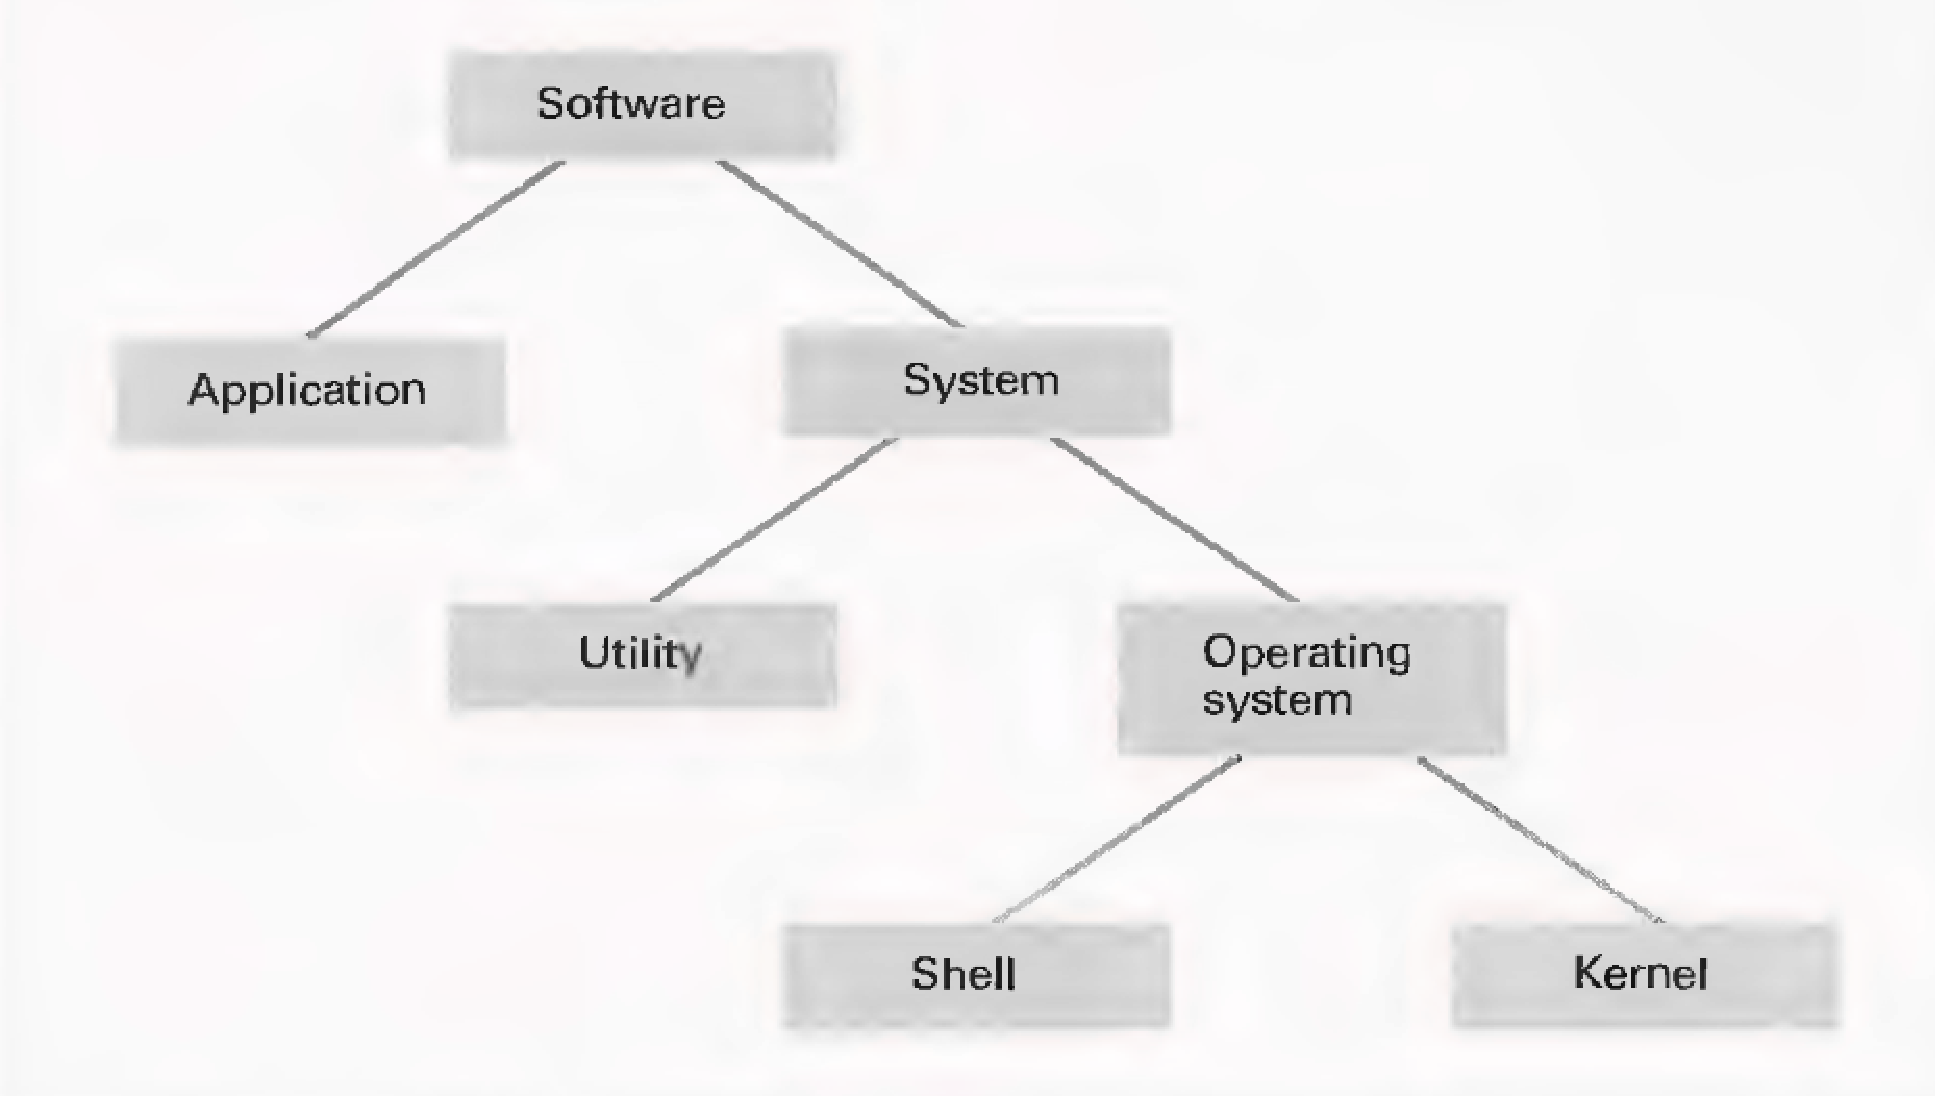
\includegraphics{ch4/fig33.pdf}}
  \caption{Phân loại phần mềm}
  \label{fig:fig3.3}
\end{figure}

Ngược lại với phần mềm ứng dụng là phần mềm hệ thống nhằm thực hiện các nhiệm vụ chung của
các hệ thống máy tính. Theo một nghĩa nào đó, phần mềm hệ thống cung cấp cơ sở hạ tầng cho
các phần mềm ứng dụng. Ta có thể ví nó với cơ sở hạ tầng của một quốc gia (chính
phủ, đường đi lại, các nghành phục vụ, viện tài chính,...) cung cấp cơ sở cho người dân
dựa vào sống theo cách của họ.

Bên trong các lớp các phần mềm hệ thống ta lại chia thành hai phạm trù: một là bản thân hệ
điều hành và hai là những phần mềm khác bao gồm các đơn vị phần mềm tập hợp lại dưới dạng
\textbf{phần mềm công cụ}. Phần lớn phần mềm công cụ cài đặt các chương trình nhằm thực
hiện các hoạt động cơ bản của máy tính nhưng không có sẵn trong hệ điều hành. Theo một
nghĩa nào đó, phần mềm công cụ bao gồm các đơn vị phần mềm giúp mở rộng (cũng có thể để
tuỳ biến) khả năng của hệ điều hành. Ví dụ, chức năng format một đĩa từ hoặc sao chép một
files từ đĩa từ vào đĩa CD thường không được cài đặt bởi hệ điều hành nhưng nó được cung
cấp bởi phần mềm công cụ. Những ví dụ khác của phần mềm công cụ là phần mềm nén và giải
nén dữ liệu, phần mềm để trình diễn đa phương tiện, và phần mềm để thực hiện truyền thông
trong mạng.

Sử dụng các phần mềm công cụ cho phép phần mềm hệ thống có thể tuỳ biến dễ dàng hơn so với
việc đặt chúng có sẵn ngay trong hệ điều hành. Thật vậy, thông thường các công ty hoặc cá
nhân phải thay đổi, hoặc thêm, các phần mềm công cụ vào hệ điều hành trong máy của họ.

Không may mắn, việc phân biệt giữa phần mềm ứng dụng và phần mềm công cụ là không rõ
ràng. Theo quan điểm của chúng tôi, sự khác biệt là gói phần mềm này có là một phần trong
cơ sở hạ tầng phần mềm của máy hay không. Bởi vậy một ứng dụng mới có thể thuộc nhánh công
cụ nếu nó trở thành một công cụ cơ bản. Khi vẫn còn là dự án nghiên cứu, phần mềm để
truyền thông trên Internet đã được xem là phần mềm ứng dụng; ngày nay phần mềm kiểu này là
cơ bản cho hầu hết việc sử dụng PC và bởi vậy nó được phân loại là phần mềm công cụ.



Sự phân biệt giữa phần mềm công cụ và hệ điều hành cũng không rõ ràng. Ví dụ, luật chống
độc quyền ở Mỹ và Châu Âu đã đặt ra câu hỏi liên quan đến phần mềm như trình duyệt web
Internet Explorer và Media Player là một thành phần của hệ điều hành của Microsoft hay chỉ
là phần mềm công cụ mà Microsoft đã cố tình cho vào hệ điều hành nhằm mục đích cạnh tranh.


\subsection*{Các thành phần của một hệ điều hành}

Ta sẽ chú tâm vào thành phần bên trong một hệ điều hành. Để có thể thực hiện các hoạt động
được yêu cầu bởi những người dùng, hệ điều hành phải có khả năng giao tiếp. Thành phần của
một hệ điều hành thực hiện việc giao tiếp này thường được gọi là \textbf{shell}. Các shell
hiện đại thực hiện nhiệm vụ này thường theo hướng \textbf{giao diện đồ hoạ với người dùng
  (GUI)} trong đó các đối tượng cần thao tác như các file và chương trình, được biểu diễn
bằng các biểu tượng trên màn hình. Các hệ thống này cho phép hiểu lệnh của người dùng
thông qua việc trỏ tới các biểu tượng này. Việc này thường được thực hiện nhờ một thiết bị
cầm tay được gọi là chuột. Các shell cũ hơn thường giao tiếp với người dùng qua thông điệp
dạng văn bản sử dụng bàn phím và màn hình.



Mặc dù shell của hệ điều hành đóng vai trò quan trọng trong việc thiết lập các chức năng
của máy, các shell này đơn thuần chỉ là giao diện giữa người dùng và nhân (trái tim) của
hệ điều hành (Hình \ref{fig:fig3.4}). Ta phân biệt giữa shell và phần bên trong của hệ
điều hành như thế này bởi vì một số hệ điều hành cho phép người dùng lựa chọn các shell
khác nhau để có một giao diện phù hợp với từng đối tượng người dùng cụ thể. Ví dụ, người
dùng hệ điều hành UNIX có thể lựa chọn một trong nhiều shell như Bourne shell, C shell, và
Korn shell. Hơn nữa, những phiên bản trước của hệ điều hành Microsoft Windows về mặt cơ
bản đã được xây dựng nhằm thay thế các shell dựa trên văn bản đang sử dụng (trên hệ điều
hành MS-DOS) bằng một shell kiểu giao diện đồ hoạ, tuy nhiên khung của nó vẫn là MS-DOS.

\begin{figure}[tb]
  \centering \scalebox{0.4}{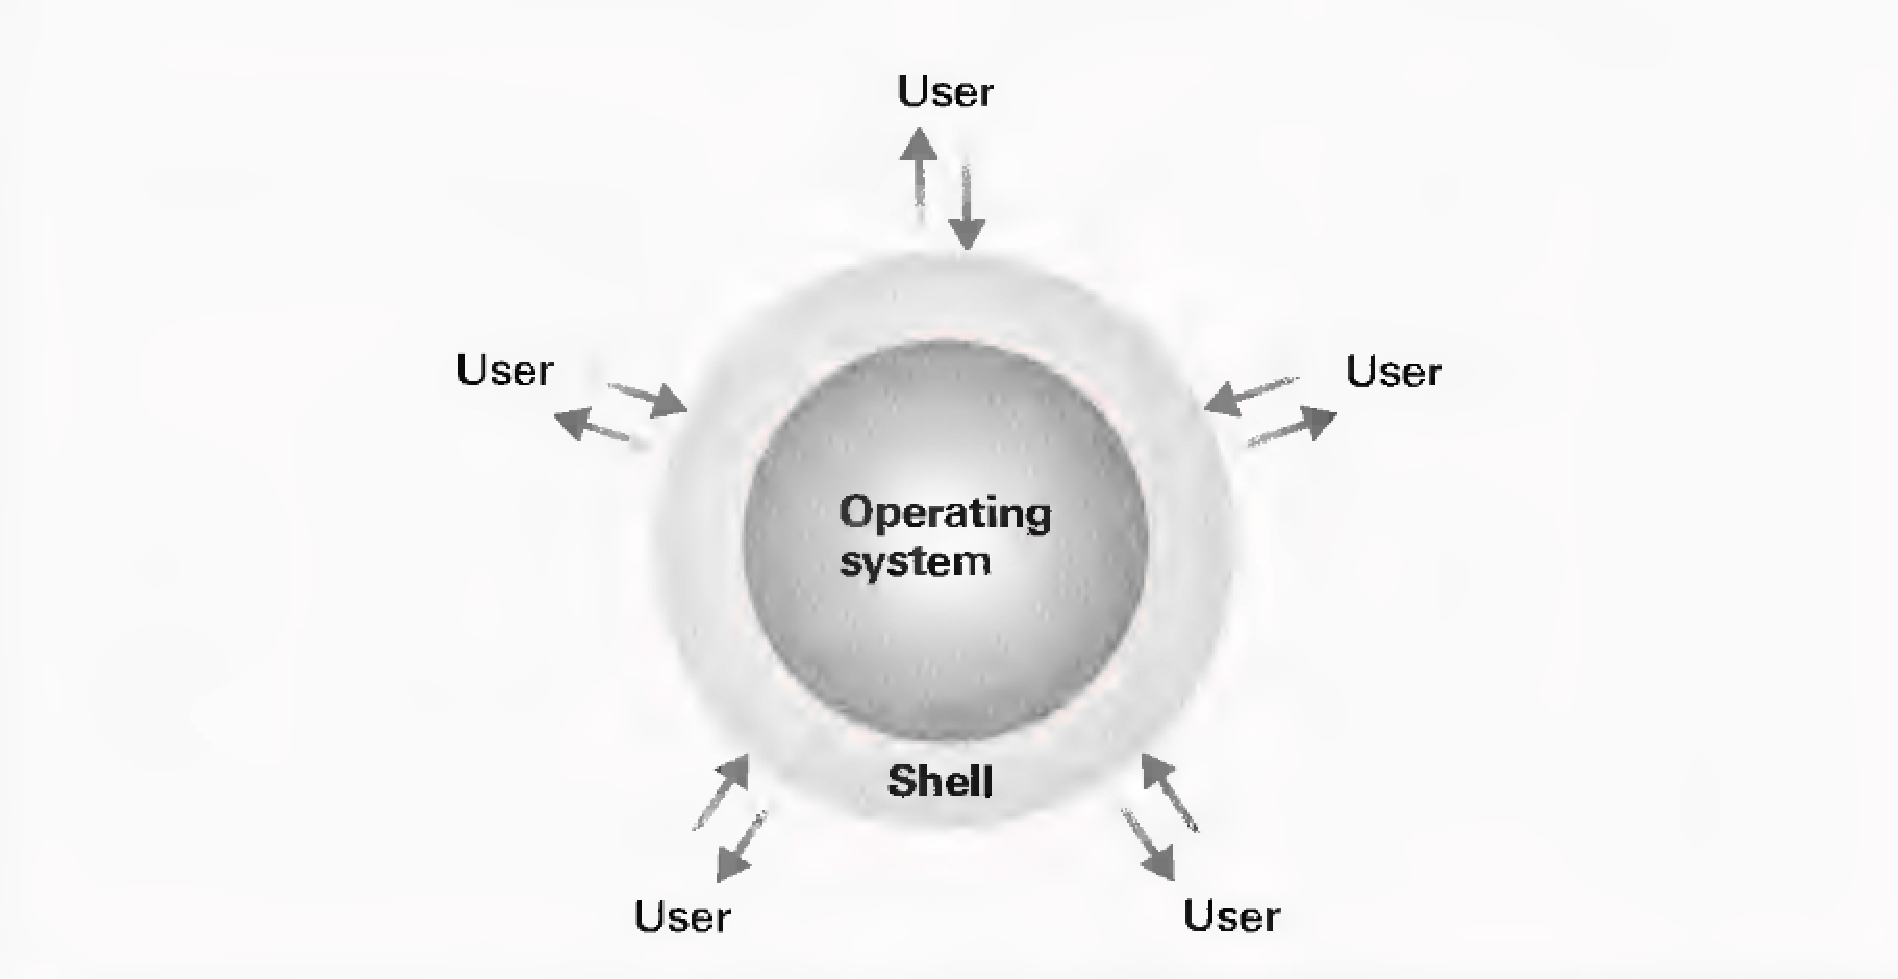
\includegraphics{ch4/fig34.pdf}}
  \caption{Shell như một giao diện giữa người dùng và hệ điều hành}
  \label{fig:fig3.4}
\end{figure}

Một thành phần quan trọng bên trong các shell đồ hoạ của ngày nay là \textbf{chương trình
  quản lý cửa sổ}, với các khối được cấp phát của không gian màn hình, được gọi là cửa sổ,
và mỗi các ứng dụng được gắn với mỗi cửa sổ. Khi một ứng dụng muốn hiện một thứ gì đó ra
màn hình, nó thông báo với trình quản lý cửa sổ, và trình quản lý cửa sổ sẽ đặt các hình
ảnh mong đợi vào trong cửa sổ gắn với ứng dụng. Từ đó, mỗi khi một nút chuột được nhấn,
chính trình quản lý cửa sổ sẽ tính toán vị trí của chuột trên màn hình và gọi ứng dựng
thích hợp tương ứng với thao tác của chuột.

Ngược lại với shell của hệ điều hành, phần bên trong của hệ điều hành được gọi là
\textbf{nhân} (kernel). Một nhân của hệ điều hành chứa các thành phần phần mềm thực hiện
các chức năng rất cơ bản yêu cầu bởi hệ thống máy tính. Một ví dụ là \textbf{trình quản lý
  file}, công việc của nó là phối hợp làm dễ dàng việc sử dụng thiết bị lưu trữ khối của
máy. Chính xác hơn, trình quản lý file chứa các bản ghi của mọi file nằm trong thiết bị
lưu trữ khối, gồm cả vị trí mỗi file được đặt, người dùng nào được phép truy cập vào file
nào, và bộ phận nào của lưu trữ khối sẵn sàng dành cho các file mới, hoặc mở rộng các file
đã tồn tại. Các bản ghi này được giữ ở một nơi lưu trữ trung gian chứa các file liên quan
sao cho mỗi thời điểm nơi trung gian được đặt trực tuyến, trình quản lý file có thể tìm
thấy chúng và biết có gì được lưu trữ ở phần trung gian này.

Để thích hợp với người dùng máy, hầu hết các trình quản lý file cho phép các file được
nhóm lại dưới dạng \textbf{thư mục} (directory hoặc folder). Cách tiếp cận này cho phép
người dùng tổ chức các file của anh hay chị ta theo mục đích bằng cách đặt các file có
liên quan trong cùng một thư mục. Hơn nữa, bằng cách cho phép các thư mục chứa các thư mục
khác, được gọi là thư mục con, một tổ chức theo kiểu phân cấp có thể được xây dựng. Ví dụ,
một người dùng tạo ra một thư mục gọi là \texttt{MyRecords} có chứa các thư mục con là
\texttt{FinancialRecord}, \texttt{MedicalRecords} và \texttt{HouseHoldRecord}. Bên trong
mỗi thư mục con có thể có các file ở một phạm trù đặc biệt (Người dùng hệ điều hành
Windows có thể hỏi trình quản lý file để hiện tập các thư mục hiện hành bằng cách thực
hiện chương trình Windows Explorer).

Một đường đi tới một thư mục bên trong các thư mục được gọi là \textbf{đường dẫn thư
  mục}. Đường dẫn thường được biểu diễn bằng cách liệt kê các thư mục dọc theo đường đi
ngăn cách bởi dấu gạch chéo. Ví dụ,  \texttt{animals/prehistoric/dinosaurs} để biểu
diễn dẫn bắt đầu từ thư mục có tên là \texttt{animals}, qua thư mục con có tên là
\texttt{prehistoric}, và kết thúc trong thư mục con \texttt{dinosaurs}. (Đối với người
dùng Windows, dấu gạch xuôi được thay bằng các dấu gạch ngược lại, ví dụ đường dẫn ở trên
được thay bằng \texttt{animals$\backslash$prehistoric$\backslash$dinosaurs}).

Mọi sự truy cập vào một file bởi một phần mềm khác phải được sự đồng ý của trình quản lý
file theo một thủ tục. Thủ tục bắt đầu bằng cách yêu cầu trình quản lý file kiểm tra quyền
truy cập tới file qua thủ tục mở file. Nếu trình quản lý file đồng ý với yêu cầu truy cập,
nó cung cấp thông tin cần để tìm và thao tác file. Thông tin này được lưu trữ trong một
vùng nhớ được gọi là \textbf{bộ mô tả file} (file descriptor). Phần mềm cần truy cập sẽ
tham khảo các thông tin trong bộ mô tả file này để thực hiện các thao tác nó mong muốn.

Các thành phần khác của nhân (kernel) hệ điều hành bao gồm một tập các \textbf{bộ điều
  khiển thiết bị}, là đơn vị phần mềm chịu trách nhiệm giao tiếp với các bộ điều khiển
(hoặc đôi khi, giao tiếp trực tiếp với thiết bị ngoại vi) để thực hiện các thao tác trên
các thiết bị ngoại vi gắn với máy. Mỗi thiết bị được thiết kế duy nhất cho một kiểu thiết
bị đặc biệt (như máy in, bộ điều khiển đĩa, hoặc màn hình). Nó có trách nhiệm dịch các yêu
cầu chung thành các bước kỹ thuật hơn được yêu cầu bởi thiết bị được gán với bộ điều
khiển. Ví dụ, một bộ điều khiển thiết bị máy in chứa các phần mềm đọc và giải mã các từ mô
tả trạng thái của máy in và các phương pháp giao tiếp kiểu bắt tay khác. Bởi vậy, các
thành phần phần mềm khác không giải quyết được về mặt kỹ thuật cho vấn đề in file. Thật
vậy, các thành phần khác có thể đơn thuần là dựa vào phần mềm điều khiển thiết bị để in
file, còn làm chi tiết thế nào nó để lại cho bộ điều khiển thiết bị. Bằng cách này, việc
thiết kế của các đơn vị phần mềm khác nhau không bị phụ thuộc vào đặc trưng của thiết bị
cụ thể. Kết quả là ta có thể tuỳ biến hệ điều hành cho các thiết bị ngoại vi đặc biệt đơn
thuần bằng cách cài gắn thêm trình điều khiển thiết bị thích hợp.

Một thành phần khác của nhân hệ điều hành là \textbf{quản lý bộ nhớ}, nó chịu trách nhiệm
điều phối việc sử dụng bộ nhớ chính. Trong môi trường đơn nhiệm (máy chỉ thực hiện một
nhiệm vụ tại một thời điểm), nhiệm vụ kiểu này là rất đơn giản. Ở đây, chương trình thực
hiện nhiệm vụ hiện hành đã được đặt trong bộ nhớ, sau khi nó thực hiện xong, bộ nhớ sẽ
được thay thế bởi chương trình thực hiện nhiệm vụ tiếp theo. Tuy nhiên, trong môi trường
đa người dùng hay đa nhiệm, ở đó máy tính phải đáp ứng nhiều yêu cầu tại cùng một thời
điểm, thì việc quản lý bộ nhớ là rất khó khăn. Trong các trường hợp này, nhiều chương
trình và khối dữ liệu phải đồng thời nằm trong bộ nhớ. Bởi thế, trình quản lý bộ nhớ phải
tìm và gán không gian bộ nhớ cho các yêu cầu này và đảm bảo rằng các hoạt động của mỗi
chương trình bị hạn chế trong không gian được cấp phát. Hơn nữa, bởi yêu cầu các hoạt động
khác nhau đến và đi liên tục, trình quản lý bộ nhớ phải nắm bắt được các vùng nhớ nào
không bị còn bận nữa.

Nhiệm vụ của trình quản lý bộ nhớ phức tạp hơn khi tổng số không gian bộ nhớ yêu cầu lớn
hơn so với không gian thực sự có trong máy tính. Trong trường hợp này trình quản lý bộ nhớ
có thể tạo ra cảm giác có không gian lưu trữ thêm bằng cách chuyển chương trình và dữ liệu
qua lại giữa bộ nhớ chính và phần lưu trữ khối (một kỹ thuật gọi là \textbf{phân
  trang}). Giả sử rằng, yêu cầu bộ nhớ chính là $1024$MB nhưng máy tính chỉ có~$512$MB. Để
tạo ra cảm giác có không gian lưu trữ lớn hơn, trình quản lý bộ nhớ dành~$1024$MB không
gian lưu trữ trên đĩa từ để lưu trữ các dãy bít có thể lưu trữ trên bộ nhớ chính nếu bộ
nhớ chính có khả năng thực sự là $1024$MB. Các dữ liệu này được chia thành các khối bằng
nhau được gọi là \textbf{các trang}, kích thuớc các trang này thường chỉ vài KB. Trình
quản lý bộ nhớ điều khiển các trang này tráo đổi giữa bộ nhớ chính và bộ nhớ thứ cấp sao
cho các trang hiện tại cần sẽ nằm trong $512$MB của bộ nhớ chính. Vậy máy tính có thể xử
lý giống như nó có $1024$MB bộ nhớ chính. Không gian bộ nhớ ``tưởng tượng'' này được tạo
bởi cách phân trang được gọi là \textbf{bộ nhớ ảo}.

Nhân hệ điều hành còn có thêm hai thành phần nữa là \textbf{bộ lập lịch} (scheduler) và
\textbf{bộ điều phối} (dispacher). Trong hệ thống chia sẻ thời gian thực, bộ lập lịch xác
định hoạt động nào được thực hiện và bộ điều phối điều khiển việc cấp phát thời gian bộ xử
lý cho các hoạt động này. Ta sẽ nghiên cứu chi tiết hai thành phần này trong mục sau.

\subsection*{Quá trình khởi động máy}
Ta đã thấy rằng hệ điều hành cung cấp cơ sở hạ tầng phần mềm cần thiết cho các đơn
vị phần mềm khác, nhưng ta chưa biết bản thân hệ điều hành bắt đầu như thế nào. Đây
chính là quá trình \textbf{khởi động}, quá trình này được thực hiện mỗi khi máy tính được
bật. Nó là thủ tục nạp hệ điều hành từ thiết bị lưu trữ thứ cấp vào trong bộ nhớ chính
(luôn là rỗng khi máy bật). Để hiểu quá trình khởi động và sự cần thiết của quá trình này,
ta bắt đầu bằng cách xem xét cấu trúc của CPU.

Một CPU được thiết kế có bộ đếm chương trình bắt đầu với một địa chỉ xác định trước mỗi
khi máy bật. Và tại đây, CPU mong đợi tìm thấy một chương trình để thực hiện. Về mặt thiết
kế, ta chỉ cần lưu trữ hệ điều hành bắt đầu tại địa chỉ này. Tuy nhiên, do tính chất của
bộ nhớ chính, dữ liệu bị mất đi sau khi tắt máy nên ta phải tìm cách nạp lại dữ liệu vào
bộ nhớ chính mỗi khi máy tính khởi động lại.

Do vậy, một phần nhỏ của bộ nhớ chính nơi CPU mong muốn tìm thấy chương trình khởi đầu của
nó được xây dựng từ kiểu bộ nhớ bền vững (không bị mất khi tắt máy) gọi là \textbf{bộ nhớ
  chỉ đọc (ROM)}, nội dung của nó không thể bị thay đổi. Tuy vậy, hầu hết bộ nhớ ROM ngày
nay được được xây dựng dựa trên công nghệ bộ nhớ flash (có nghĩa rằng nó không hoàn toàn
là ROM bởi vì nó cho phép ghi lại trong trường hợp cần thiết).



Chương trình được lưu trữ trong ROM gọi là \textbf{chương trình mồi}. Chương trình này
được thực hiện một cách tự động khi máy được bật. Nó có nhiệm vụ điều khiển CPU nạp hệ
điều hành từ vị trí xác định trước trong bộ nhớ thứ cấp (thường là đĩa từ) vào bộ nhớ
chính (xem Hình~\ref{fig:fig3.5}). Khi hệ điều hành đã được đặt trong bộ nhớ chính, chương
trình mồi thực hiện một lệnh nhảy đến vùng nhớ này. Lúc này hệ điều hành tiếp quản và bắt
đầu điều khiển các hoạt động của máy.

\begin{figure}[tb]
  \centering \scalebox{0.35}{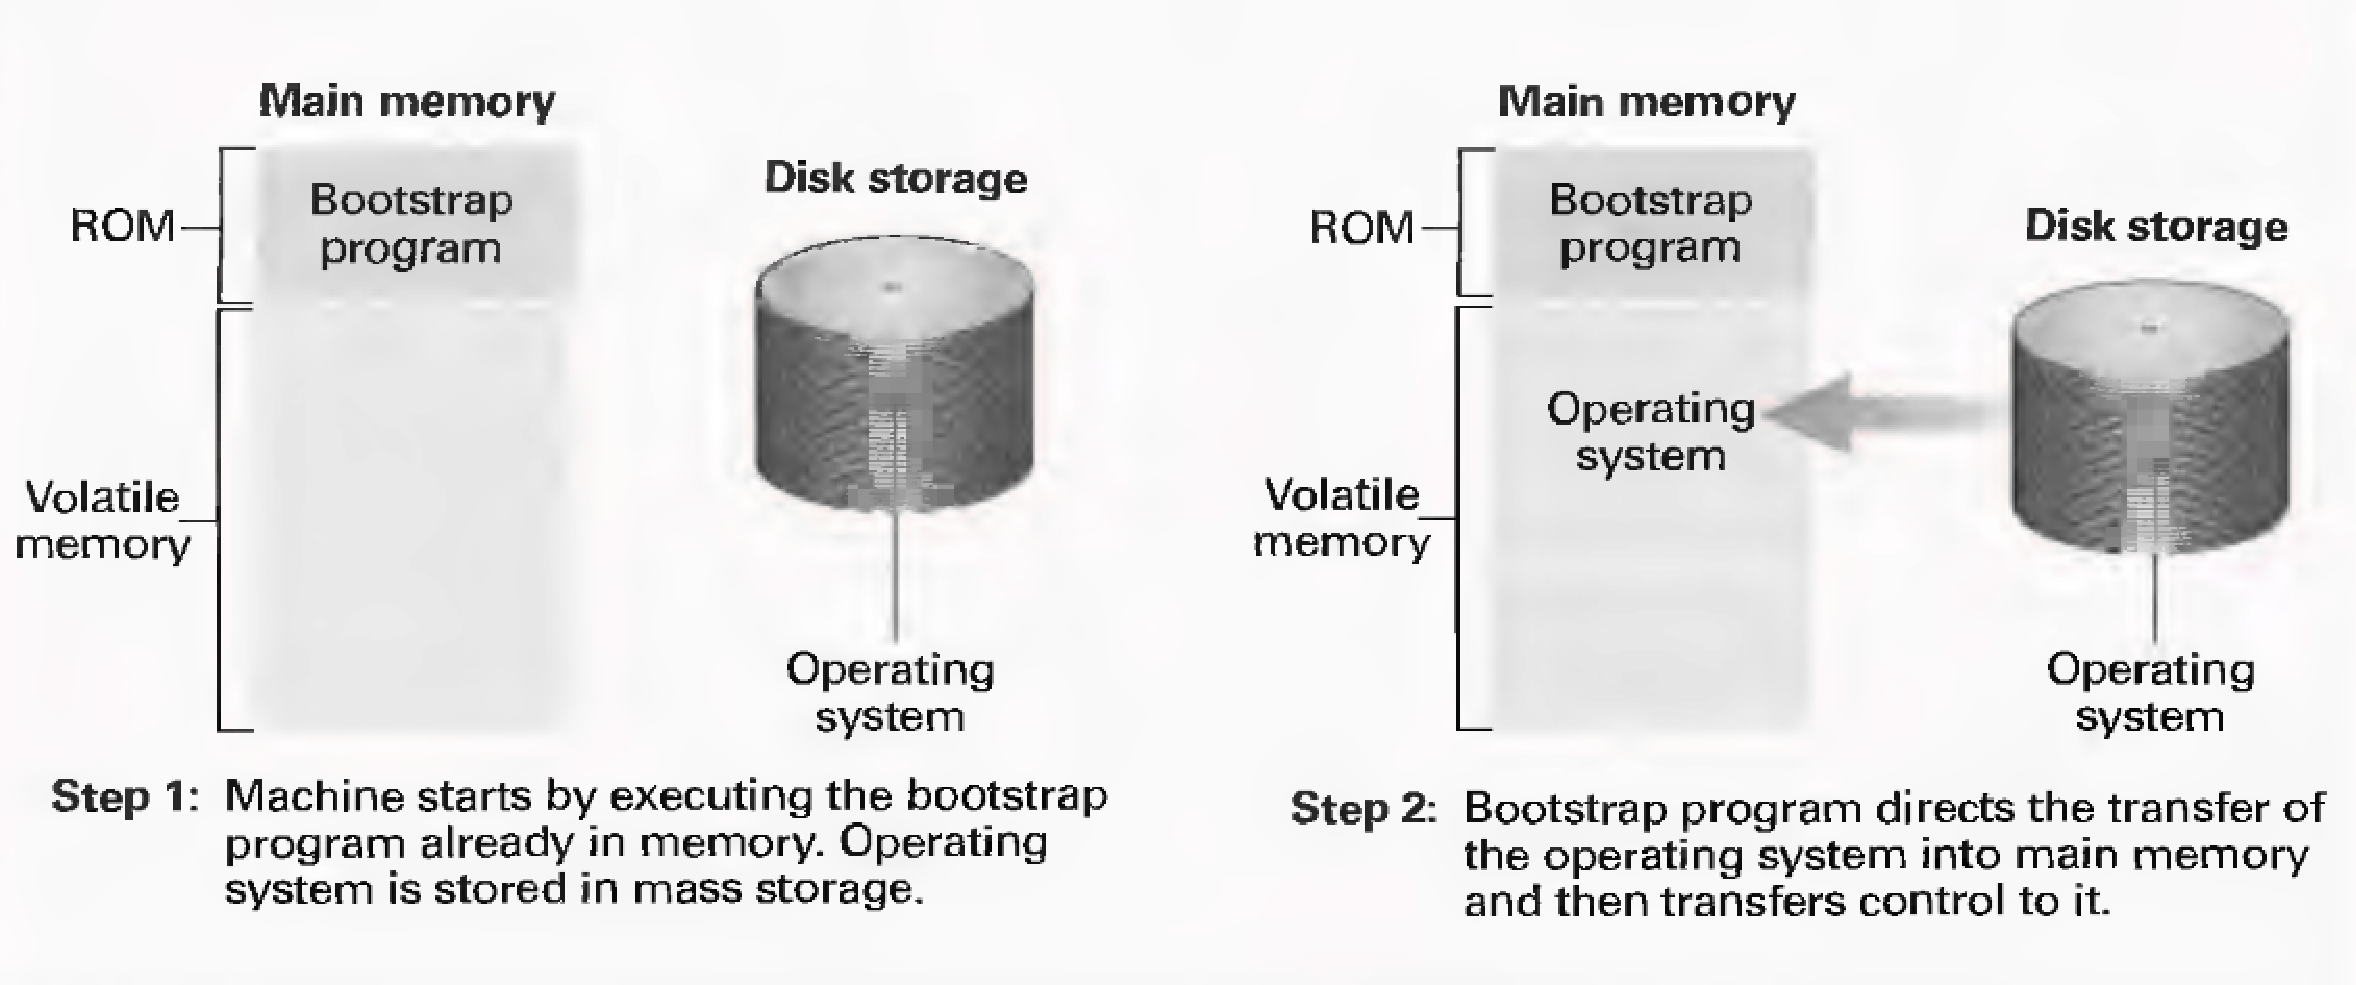
\includegraphics{ch4/fig35.pdf}}
  \caption{Quá trình khởi động}
  \label{fig:fig3.5}
\end{figure}



Một câu hỏi là tại sao không cung cấp đủ ROM để lưu trữ toàn bộ hệ điều hành để tránh phải
nạp từ bộ nhớ thứ cấp. Câu trả lời là do công nghệ hiện tại chưa cho phép dành hẳn một
vùng nhớ lớn của bộ nhớ chính làm vùng lưu trữ bền vững. Tuy nhiên, với sự phát triển
nhanh chóng của công nghệ bộ nhớ, quá trình khởi động mất nhiều bước như thế sẽ sớm trở
nên lạc hâu, và thay vào đó là cách tiếp cận cho phép các phần mềm được lưu trữ lâu bền
trong bộ nhớ.

\subsection*{Câu hỏi \& Bài tập}
\begin{enumerate}
\item Liệt kê các thành phần của một hệ điều hành điển hình và tóm tắt vai trò của mỗi
  thành phần trong một câu.

\item Chỉ ra sự khác nhau giữa phần mềm ứng dụng và phần mềm công cụ.

\item Bộ nhớ ảo là gì?

\item Tóm tắt quá trình khởi động máy.
\end{enumerate}

\section{Điều phối các hoạt động của máy}

Trong phần này ta xem xét cách một hệ điều hành điều phối việc thực hiện phần mềm ứng
dụng, phần mềm công cụ, và bản thân các đơn vị bên trong hệ điều hành. Ta bắt đầu với khái
niệm tiến trình.

\subsection*{Khái niệm tiến trình}
Một trong những khái niệm cơ bản nhất của hệ điều hành hiện đại là phân biệt giữa một
chương trình và hoạt động thực hiện chương trình. Chương trình là một tập tĩnh các chỉ
thị, trong khi đó hoạt động thực hiện chương trình là động, và thay đổi theo thời gian khi
chương trình chạy. Hoạt động này được gọi là \textbf{tiến trình}. Gắn với một tiến trình
là trạng thái hiện hành của hoạt động, được gọi là \textbf{trạng thái của tiến
  trình}. Trạng thái này bao gồm vị trí hiện tại của chương trình đang thực hiện (giá trị
của bộ đếm chương trình) cũng như các giá trị của các thanh ghi và các ô nhớ gắn với
nó. Nói nôm na, trạng thái tiến trình là một ảnh chụp nhanh (snapshot) của máy tại một
thời điểm cụ thể. Những thời điểm khác nhau trong lúc thực hiện chương trình (tại các thời
điểm khác nhau trong một tiến trình) ta quan sát được các ảnh chụp khác nhau (trạng thái
khác nhau của tiến trình).


Trong một hệ thống chia sẻ thời gian thực, thường có nhiều tiến trình tranh chấp tài
nguyên của máy. Nhiệm vụ của hệ điều hành là phải quản lý các tiến trình này sao cho mỗi
tiến trình có tài nguyên (thiết bị ngoại vi, không gian trong bộ nhớ chính, truy cập các
file, và truy cập vào CPU) nó cần, sao cho các tiến trình độc lập không gây trở ngại lẫn
nhau, và sao cho các tiến trình có thể trao đổi thông tin nếu cần.

\subsection*{Quản lý tiến trình}

Các nhiệm vụ liên quan đến việc điều phối tiến trình được thực hiện bởi bộ lập lịch và bộ
điều phối trong nhân của hệ điều hành. Bộ lập lịch duy trì thông tin về tiến trình có mặt
trong hệ thống, đưa các tiến trình mới vào hàng đợi, loại bỏ các tiến trình đã hoàn thành
ra khỏi hệ thống. Bởi vậy, khi người dùng yêu cầu thực hiện một ứng dụng, chính bộ lập
lịch thêm việc thực hiện ứng dụng vào danh sách các tiến trình hiện thời.

Để lưu vết mọi tiến trình, bộ lập lịch duy trì một khối thông tin trong bộ nhớ chính gọi
là \textbf{bảng các tiến trình}. Mỗi khi có yêu cầu thực hiện một chương trình, bộ lập
lịch thêm một mục mới vào trong bảng tiến trình cho tiến trình này. Mục này chứa các thông
tin như vùng bộ nhớ được gán cho tiến trình (lấy từ chương trình quản lý bộ nhớ), độ ưu
tiên của các tiến trình, và trạng thái tiến trình sẵn sàng hay đang đợi. Một tiến trình là
\textbf{sẵn sàng} nếu nó ở trạng thái có thể tiếp tục chạy; nó là \textbf{đợi} nếu hiện
tại nó đang phải đợi cho đến khi một vài sự kiện nào đó bên ngoài xuất hiện, như việc truy
cập đĩa đã hoàn thành, nhấn một phím trên bàn phím, hoặc một thông điệp đến từ tiến trình
khác.



Bộ điều phối tiến trình là thành phần của nhân hệ điều hành chịu trách nhiệm đảm bảo tiến
trình được lập lịch thực sự được thực hiện. Trong hệ thống chia sẻ thời gian thực nhiệm vụ
này được kèm với việc \textbf{chia sẻ thời gian}; có nghĩa rằng, chia thời gian thành
những khoảng ngắn, mỗi khoảng gọi là \textbf{time slide} (thông thường khoảng $50$ mili
giây), và chuyển đổi sự chú ý của CPU tới mỗi tiến trình cho phép mỗi tiến trình thực hiện
trong một time slide (Hình \ref{fig:fig3.6}). Thủ tục chuyển từ tiến trình này sang tiến
trình khác gọi là \textbf{chuyển đổi tiến trình} (process switch) hay \textbf{chuyển ngữ
  cảnh} (context switch).

\begin{figure}[bt]
  \centering \scalebox{0.35}{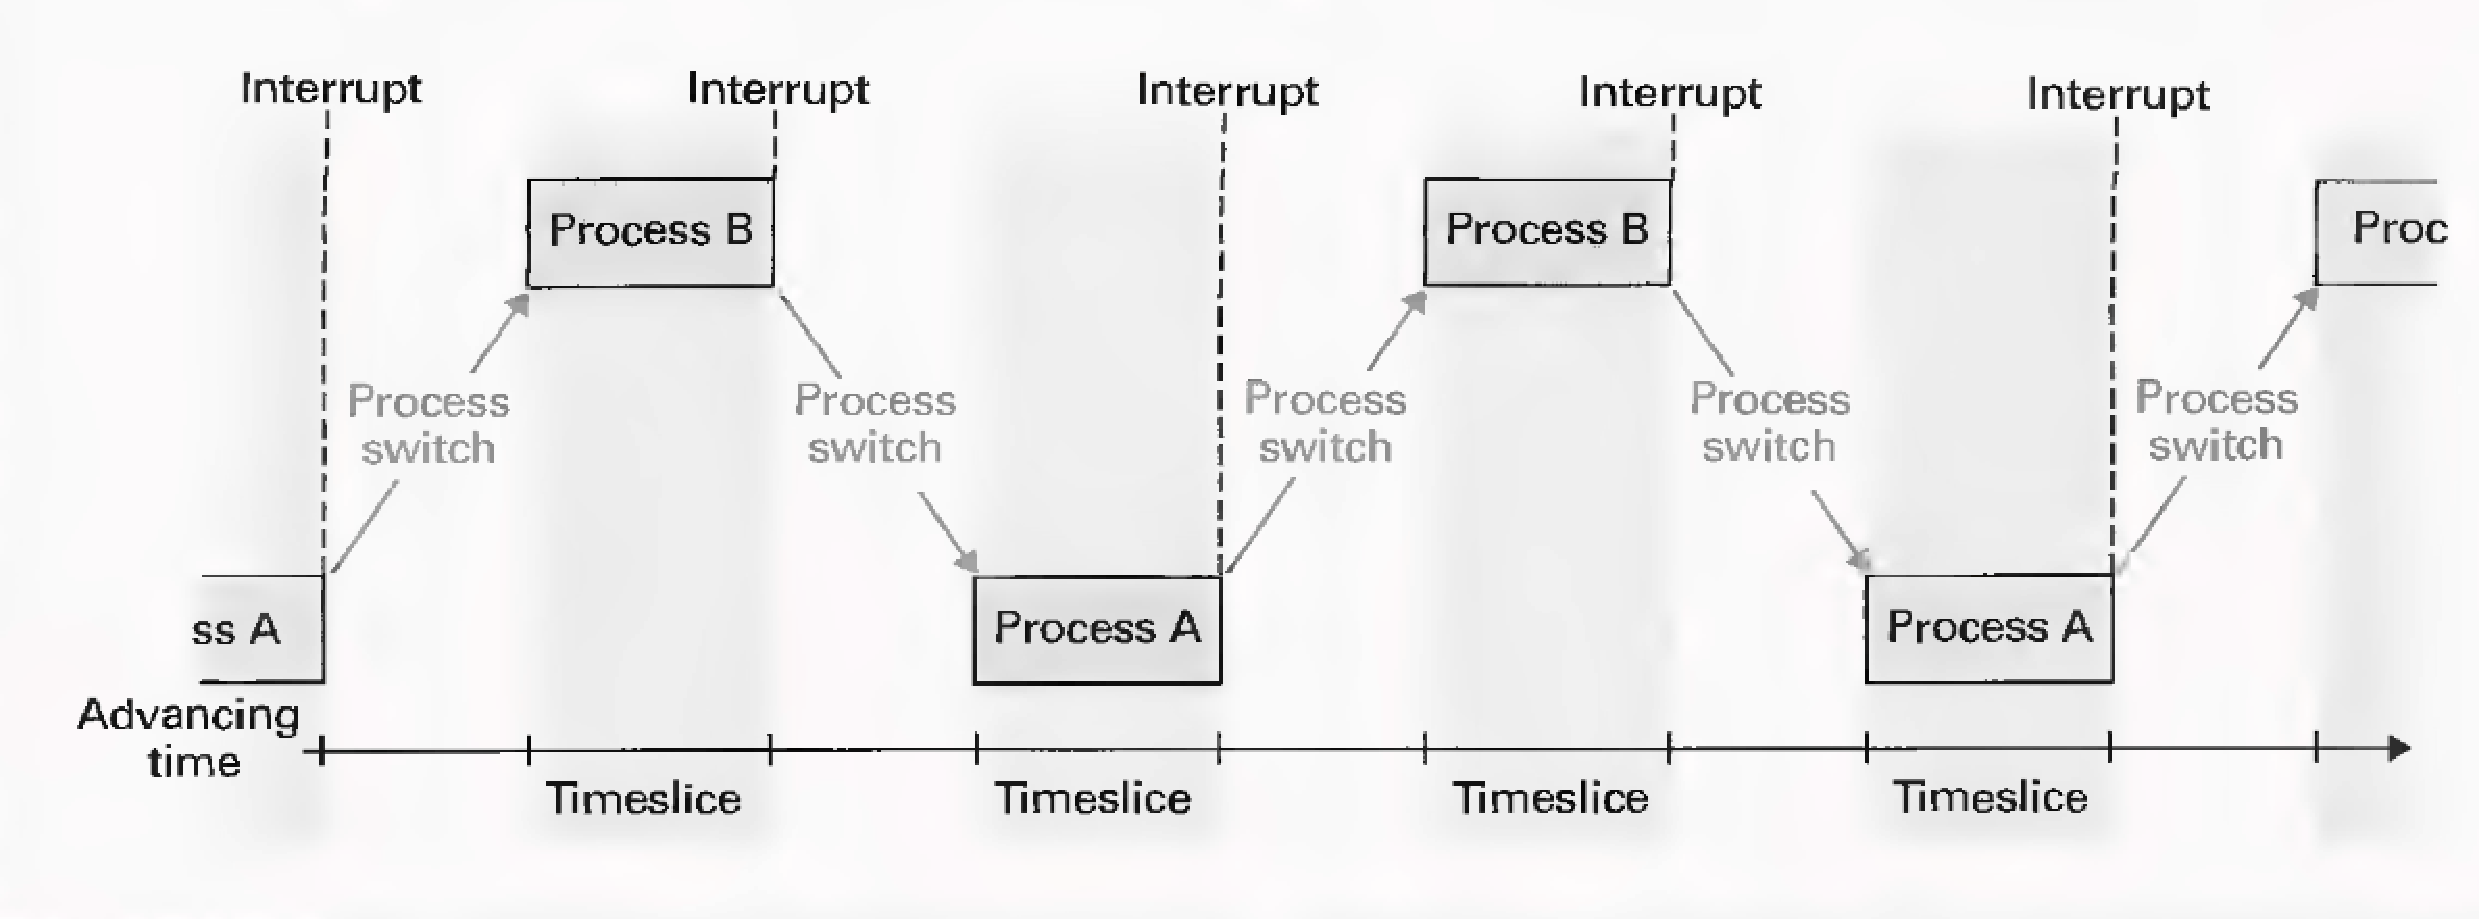
\includegraphics{ch4/fig36.pdf}}
  \caption{Chia sẻ thời gian thực giữa tiến trình $A$ và tiến trình $B$}
  \label{fig:fig3.6}
\end{figure}


Mỗi khi bộ điều phối tiến trình trao time slide cho một tiến trình, nó khởi tạo một mạch
thời gian. Mạch này sẽ sinh ra một tín hiệu gọi là \textbf{ngắt} (interrupt) mỗi khi kết
thúc một time slide. CPU phản hồi lại tín hiệu ngắt này giống như bạn phản ứng khi bị dừng
một công việc. Bạn dừng việc bạn đang làm, ghi nhận lại chỗ công việc bị dừng (để bạn có
thể tiếp tục làm sau), và chuyển sự quan tâm đến đối tượng đòi bạn phải tạm dừng công
việc. Khi CPU nhận một tín hiệu ngắt, nó hoàn thành chu kỳ máy hiện thời của nó, ghi lại
vị trí hiện thời của tiến trình và bắt đầu thực hiện một chương trình, được gọi là
\textbf{trình xử lý ngắt}. Chương trình này được lưu giữ ở một vị trí được xác định trước
trong bộ nhớ chính. Trình xử lý ngắt này là một phần của bộ điều phối, và nó chỉ ra cách
bộ điều phối phải trả lời tín hiệu ngắt.

Bởi vậy, ảnh hưởng của tín hiệu ngắt là để chiếm quyền ưu tiên của tiến trình hiện thời và
chuyển quyền điều khiển lại cho bộ điều phối. Đầu tiên, bộ điều phối cho phép bộ lập lịch
cập nhật bảng các tiến trình (ví dụ, độ ưu tiên của tiến trình vừa hoàn thành time slide
phải thấp hơn độ ưu tiên của các tiến trình khác vừa được đưa vào). Sau đó, bộ điều phối
lựa chọn tiến trình đang sẵn sàng và có độ ưu tiên cao nhất trong bảng các tiến trình,
khởi động lại mạch thời gian, và cho phép tiến trình vừa được lựa chọn bắt đầu time slide
của nó.

Điểm hết sức quan trọng quyết định sự thành công của hệ thống chia sẻ thời gian thực là
khả năng dừng một tiến trình, và sau đó cho phép nó chạy lại. Nếu bạn bị ngắt trong khi
đang đọc sách, khả năng để bạn đọc tiếp sau đó phụ thuộc vào khả năng nhớ vị trí trong
sách cũng như thông tin bạn đã tích luỹ được tính đến thời điểm đó. Nói ngắn gọn, bạn phải
có thể tái tạo lại được môi trường trước thời điểm bị ngắt.

Trong trường hợp của tiến trình, môi trường phải được tái tạo lại là trạng thái của tiến
trình. Nhắc lại rằng trạng thái này bao gồm giá trị của bộ đếm chương trình cũng như nội
dung của các thanh ghi và các ô nhớ thích hợp. Các CPU được thiết kế cho hệ thống chia sẻ
thời gian thực có khả năng kết hợp nhiệm vụ lưu giữ các thông tin này như một phần của
việc phản hồi lại của CPU với tín hiệu ngắt. Các CPU này cũng có các lệnh máy để nạp lại
trạng thái được lưu trữ trước đó. Các đặc điểm này đơn giản hoá nhiệm vụ của bộ điều phối
khi thực hiện chuyển đổi tiến trình và cũng là một ví dụ cho thấy việc thiết kế các CPU
hiện đại bị ảnh hưởng bởi nhu cầu của các hệ điều hành thế nào.

Cuối cùng, ta cũng để ý rằng việc chia sẻ thời gian thực làm tăng hiệu quả của hệ thống về
mặt tổng thể. Điều này đôi khi ngược lại với trực giác của ta vì việc chuyển đổi giữa các
tiến trình yêu cầu bởi hệ thời gian thực làm tốn thời gian của CPU. Tuy nhiên, nếu không
chia sẻ thời gian thực, mỗi tiến trình sẽ phải hoàn thành việc thực hiện trước khi tiến
trình tiếp theo bắt đầu, có nghĩa rằng thời gian tiến trình đợi thiết bị ngoại vi hoàn
thành hoặc đợi yêu cầu từ người sử dụng là bị lãng phí. Còn nếu chia sẻ thời gian thực sẽ
cho phép chuyển CPU đang đợi cho tiến trình khác. Ví dụ, nếu một tiến trình thực hiện một
yêu cầu vào/ra, ví dụ yêu cầu lấy dữ liệu từ đĩa, bộ lập lịch sẽ cập nhật bảng tiến trình
để phản ánh rằng tiến trình này đang đợi một sự kiện bên ngoài. Vậy, bộ điều phối sẽ cắt
time slide của tiến trình này. Sau đó (có thể đến vài nghìn mili giây), khi yêu cầu vào/ra
được hoàn thành, bộ lập lịch sẽ cập nhật bảng tiến trình để chỉ ra rằng tiến trình là sẵn
sàng, và bởi vậy tiến trình này sẽ một lần nữa cạnh tranh để lấy time slides. Tóm lại, một
tiến trình vẫn có thể được thực hiện trong khi yêu cầu vào/ra đang được thực hiện. Bởi
vậy, các nhiệm vụ sẽ được hoàn thành mất ít thời gian hơn so với thực hiện theo cách tuần
tự.

\subsection*{Câu hỏi \& Bài tập}
\begin{enumerate}
\item Tóm tắt sự khác nhau giữa chương trình và tiến trình.

\item Tóm tắt các bước được thực hiện bởi CPU khi một ngắt xuất hiện.

\item Trong hệ thống chia sẻ thời gian, làm thế nào các tiến trình có
  độ ưu tiên cao được phép chạy nhanh hơn so với các tiến trình khác?

\item Nếu mỗi time slide trong hệ thống chia sẻ thời gian là $50$
  milli giây và mỗi việc chuyển đổi ngữ cảnh yêu cầu ít nhất một micro
  giây, có bao nhiêu tiến trình có thể được phục vụ trong một giây?
\label{ex:3.3.4}

\item Nếu mỗi tiến trình sử dụng đầy đủ time slide của nó theo máy ở
  Bài tập \ref{ex:3.3.4}, khoảng thời gian nào của máy thực sự dành
  cho việc thực hiện tiến trình? khoảng thời gian của máy thực sự dành
  cho thực hiện tiến trình là bao nhiêu nếu mỗi tiến trình thực hiện
  một yêu cầu vào/ra chỉ sau một micro giây time slide của nó?
\end{enumerate}







%%% Local Variables: 
%%% mode: latex
%%% TeX-master: "../tindaicuong"
%%% End: 


\section{An ninh của máy tính}

Bởi vì các hệ điều hành giám sát các hoạt động của máy tính, nên nó cũng đóng vai trò
chính trong việc đảm bảo an ninh. Theo nghĩa rộng, nó có thể ở nhiều dạng, một trong số
chúng là độ tin cậy. Nếu sai sót trong trình quản lý file gây ra mất dữ liệu của file, vậy
file không an toàn. Nếu chương trình điều phối gây ra đổ vỡ hệ thống, làm mất dữ liệu ta
mất cả giờ để đánh, vậy công việc của ta không an toàn. Bởi vậy, an ninh của một hệ
thống tính toán đòi hỏi hệ điều hành phải được thiết kế tốt và đáng tin cậy.

Việc phát triển các phần mềm đáng tin cậy không phải là vấn đề nghiên cứu của hệ điều
hành. Nó thuộc phạm vi của Công nghệ phần mềm, ta sẽ xem xét sau trong
Chương~\ref{}. Trong phần này, ta chỉ quan tâm đế các vấn đề an ninh liên quan riêng đến
hệ điều hành.

\subsection*{Tấn công từ bên ngoài}
Một trong những nhiệm vụ quan trọng của hệ điều hành là bảo vệ tài nguyên của máy tính
tránh khỏi các truy cập bất hợp lệ. Trong trường hợp hệ thống có nhiều người sử dụng, việc
bảo vệ này dựa trên ``tài khoản'' (account)--một tài khoản được quản lý trong trong hệ
điều hành như một mục gồm tên người dùng, mật khẩu và quyền truy cập gắn với người
dùng. Hệ điều hành dùng các thông tin này trong mỗi lần đăng nhập (login) để điều khiển
việc truy cập vào hệ thống.

Các tài khoản được tạo bởi một người gọi là \textbf{super user} hay \textbf{người quản
  trị} (administrator). Người này có quyền cao nhất trong hệ thống, và cũng phải đăng nhập
vào hệ thống để xác thực anh/chị ta là người quản trị (thường bởi tên và mật khẩu). Khi đã
đăng nhập, người quản trị có thể làm nhiều thay đổi bên trong hệ thống như: thay đổi gói
phần mềm, gán quyền cho người dùng, thực hiện các hoạt động bảo trì hệ thống,...

Dùng ``quyền rất cao'' này, người quản trị phải điều khiển hoạt động trong hệ thống để
kiểm tra các hành vi phá hoại hệ thống, do vô tình hay cố ý. Cũng có nhiều phần mềm công
cụ trợ giúp người quản trị, được gọi là \textbf{phần mềm kiểm tra} (auditing software). Nó
ghi lại và phân tích các hoạt động xảy ra bên trong hệ thống. Ví dụ, phần mềm kiểm tra có
thể cho biết những lần đăng nhập sai mật khẩu. Phần mềm kiểm tra cũng phát hiện các hoạt
động của một tài khoản người dùng không phù hợp với các hành vi của anh ta trong quá khứ,
để từ đó chỉ ra những người dùng không có thẩm quyền đã giành được quyền truy cập vào tài
khoản này. (ví dụ, với một người dùng bình thường chỉ dùng gói phần mềm xử lý văn bản và
bảng tính, bây giờ lại dùng các ứng dụng phần mềm kỹ thuật cao hoặc thực hiện các gói công
cụ không hợp lệ với quyền của anh ta.)

Phần mềm kiểm tra cũng được thiết kế để phát hiện các \textbf{phần mềm sniffing}, là phần
mềm khi được phép chạy trên hệ thống sẽ tìm cách ghi lại các hoạt động và sau đó thông báo
lại cho kẻ thâm nhập (intruder). Một ví dụ tuy cũ nhưng được biết rộng rãi là một chương
trình một phỏng thủ tục đăng nhập của hệ điều hành. Các chương trình như thế này có thể
làm cho người dùng khác nhầm tưởng họ đang giao tiếp với hệ điều hành, và cung cấp tên và
mật khẩu cho kẻ mạo danh.

Với mọi sự phức tạp về mặt kỹ thuật được gắn với máy tính, thật đáng ngạc nhiên là rào cản
chính của an ninh của máy tính là do sự thiếu thận trọng của người dùng. Họ chọn các mật
khẩu rất dễ đoán (như tên và ngày sinh), họ chia sẻ mật khẩu của họ với bạn bè, họ không
thay đổi mật khẩu thường xuyên, họ đưa các thiết bị lưu trữ khối off-line của mình đến chỗ
hỏng hóc khi họ chuyển các thiết bị này giữa các máy, họ cài đặt các phần mềm có thể gây
mất an toàn vào hệ thống. Để giải quyết những vấn đề này, hầu hết các hệ thống máy tính
lớn đều bắt ép người dùng tuân theo một số yêu cầu về an toàn để nâng cao ý thức trách
nhiệm của họ.

\subsection*{Tấn công từ bên trong}
Khi một kẻ thâm nhập (có thể là người dùng hợp lệ nhưng có ý đồ xấu) tấn công vào hệ
thống, chúng thường tìm cách thăm dò, tìm các thông tin quan tâm, hoặc cài đặt vào hệ
thống các phần mềm phá hoại. Điều này rất đơn giản nếu kẻ rình mò có thể truy cập hệ thống
bằng tài khoản của người quản trị. Đây chính là lý do tại sao mà mật khẩu của người quản
trị phải được bảo vệ một cách nghiêm ngặt. Tuy nhiên, nếu truy cập được vào tài khoản
người dùng thông thường, kẻ thâm nhập phải tìm cách làm đánh lừa hệ điều hành để truy cập
vào các vùng bị cấm. Ví dụ, kẻ truy cập có thể đánh lừa trình quản lý bộ nhớ cho phép một
tiến trình truy cập ra ngoài vùng nhớ dành cho nó, hoặc kẻ truy cập có thể cố gắng đánh
lừa trình quản lý file để lấy các file mà nó không có quyền truy cập.


Các CPU hiện đại được thiết kế có thêm các đặc tính nhằm ngăn chặn những vấn đề này. Ví
dụ, có thể xét nhu cầu hạn chế một tiến trình chỉ được truy cập vào vùng bộ nhớ mà trình
quản lý bộ nhớ gán cho nó; nếu không hạn chế, một tiến trình có thể xoá hệ điều hành trong
bộ nhớ chính và chiếm quyền điều khiển máy tính. Để ngăn chặn vấn đề này, các CPU được
thiết kế cho hệ điều hành đa nhiệm có thể chứa các thanh ghi đặc biệt cho phép hệ điều
hành lưu giữ các giới hạn trên và dưới của vùng nhớ được gán cho tiến trình. Và trong khi
thực hiện xử lý, CPU so sánh mỗi vùng nhớ được tham chiếu đến với các thanh ghi này để đảm
bảo nó nằm trong giới hạn cho phép. Nếu vùng nhớ tham chiếu đến vượt ra ngoài giới hạn
này, CPU tự động chuyển quyền điều khiển tới hệ điều hành (bằng cách thực hiện một dãy các
ngắt) để hệ điều hành có các xử lý phù hợp.

Dù đặc điểm ta mô tả ở trên có vẻ rất tinh tế, nhưng trên thực tế nó vẫn có vấn đề. Nếu
CPU không có thêm một vài đặc tính an toàn nữa, một tiến trình vẫn có thể truy cập vào các
ô nhớ bất hợp lệ bằng cách thay đổi thanh ghi đặc biệt (chứa giới hạn bộ nhớ). Có nghĩa
rằng, một tiến trình có thể truy cập một bộ nhớ bên ngoài đơn thuần bằng cách thay đổi các
giá trị trong thanh ghi chứa giới hạn trên và dưới của bộ nhớ, và do đó nó có thể sử dụng
không gian bộ nhớ thêm mà không cần hệ điều hành cho phép.

Để tránh các hoạt động kiểu này, CPU được thiết kế để có thể thực hiện trong một hoặc hai
\textbf{mức đặc quyền} (privilege level); ta sẽ gọi là ``mode đặc quyền'' và ``mode
không đặc quyền.'' Khi ở trong mode đặc quyền, CPU có thể thực hiện mọi lệnh có trong ngôn
ngữ máy của nó. Tuy nhiên, khi ở trong mode không đặc quyền, các lệnh mà nó có thể thực
hiện sẽ bị giới hạn. Các lệnh chỉ được phép chạy ở mode đặc quyền gọi là \textbf{lệnh đặc
  quyền}. (ví dụ lệnh đặc quyền điển hình là lệnh làm thay đổi nội dung các thanh ghi giới
hạn bộ nhớ và các lệnh làm thay đổi mode đặc quyền của CPU.) Mọi nỗ lực thực hiện một lệnh
đặc quyền khi CPU ở mode không đặc quyền đều gây ra một ngắt. Ngắt này chuyển CPU tới mode
đặc quyền và chuyển quyền điều khiển tới trình xử lý ngắt của hệ điều hành.

Khi máy được bật, CPU ở mode đặc quyền. Bởi vậy, khi kết thúc quá trình khởi động và hệ
điều hành chiếm quyền điều khiển, lúc này mọi lệnh máy đều có thể được hiện. Tuy nhiên,
mỗi khi hệ điều hành cho phép một tiến trình chạy một time slide, nó chuyển CPU tới mode
không đặc quyền bằng cách thực hiện một lệnh ``chuyển mode đặc quyền''. Và từ lúc này, hệ
điều hành sẽ được thông báo nếu tiến trình cố gắng thực hiện lệnh ở mode đặc quyền.

Các lệnh đặc quyền và điều khiển các mức đặc quyền là các công cụ chính sẵn có để các hệ
điều hành quản lý an ninh. Tuy nhiên, việc sử dụng các công cụ này là một công việc hết
sức phức tạp trong thiết kế hệ điều hành. Một lỗi nhỏ trong điều khiển mức đặc quyền có
thể gây ra thảm hoạ do những người lập trình có ý đồ xấu hoặc do các lỗi vô ý gây ra khi
lập trình. Nếu một tiến trình được phép thay đổi thay đổi bộ định thời gian điều khiển
việc chia sẻ thời gian thực của hệ thống có thể cho phép một tiến trình mở rộng time slide
và chiếm quyền điều khiển máy. Nếu một tiến trình được phép truy cập trực tiếp vào thiết
bị ngoại vi, vậy nó có thể đọc các file mà không bị giám sát bởi trình quản lý file. Nếu
một tiến trình được phép truy cập vào các ô nhớ bên ngoài vùng cho phép, nó có thể đọc và
thậm chí thay đổi dữ liệu đang được sử dụng bởi tiến trình khác.
  
\subsection*{Câu hỏi \& Bài tập}
\begin{enumerate}
\item Hãy cho vài ví dụ về việc chọn mật khẩu kém an toàn và giải thích tại sao chúng lại
  kém?

\item Các bộ xử lý của Intel sử dụng bốn mức đặc quyền. Tại sao người thiết kế lại quyết
  định dùng bốn mà không phải là ba hay năm mức?

\item Nếu một tiến trình trong hệ thống chia sẻ thời gian thực có thể truy cập vào vùng
  nhớ không được phép, làm thế nào nó có thể chiếm quyền điều khiển máy?
\end{enumerate}
%%% Local Variables: 
%%% mode: latex
%%% TeX-master: "../tindaicuong"
%%% End: 

\section{Bài tập cuối chương}
  

\begin{multicols}{2}
  \begin{enumerate}
  \item Liệt kê bốn hoạt động của một hệ điều hành điển hình.

  \item Tóm tắt sự khác nhau giữa xử lý theo lô và xử lý tương tác.

  \item Ta đặt (theo thứ tự) ba phần tử $R, S$ và $T$ vào trong một
    hàng đợi. Đầu tiên, ta lấy hai phần tử ra khỏi hàng đợi và đặt
    thêm một phần tử $X$ vào hàng đợi. Sau đó, ta lại lấy tiếp hai
    phần tử ra khỏi hàng đợi, và lại đặt thêm hai phần tử $Y, Z$ (theo
    thứ tự) vào hàng đợi, và sau đó lấy hết các phần tử cho đến khi
    hàng đợi rỗng. Hãy liệt kê các phần tử trong hàng đợi theo thứ tự
    mà chúng bị lấy ra.

  \item Chỉ ra sự khác biệt giữa xử lý tương tác và xử lý thời gian
    thực.

  \item Hệ điều hành đa nhiệm là gì?

  \item Giả sử bạn có một máy PC, hãy chỉ ra một vài tình huống bạn
    thấy rõ lợi thế của khả năng đa nhiệm của nó.

  \item Hãy chỉ ra hai phần mềm ứng dụng và hai phần mềm công cụ mà
    bạn quen thuộc.

  \item Cấu trúc thư mục được mô tả bởi đường dẫn X/Y/Z là gì?

  \item Bảng mô tả tiến trình chứa những thông tin gì?

  \item Chỉ ra sự khác nhau giữa tiến trình sẵn sàng và tiến trình
    đang đợi.

  \item Nêu sự khác nhau giữa bộ nhớ ảo và bộ nhớ chính.

  \item Giả sử máy tính của bạn có $512$MB (MiB) bộ nhớ chính, và một
    hệ điều hành cần tạo một bộ nhớ ảo gấp hai lần kích thước bộ nhớ
    chính với kích thước các trang được dùng là $2$KB (KiB). Có bao
    nhiêu trang có thể được yêu cầu.

  \item Vấn đề phức tạp gì xảy ra trong hệ thống chia sẻ thời gian
    thực nếu hai tiến trình yêu cầu truy cập vào cùng một file tại
    cùng một thời điểm? Có trường hợp nào mà trình quản lý file nên
    cho phép các yêu cầu kiểu này? Có trường hợp nào mà trình quản lý
    file nên cấm các yêu cầu kiểu này?

  \item Định nghĩa cân bằng tải và tỷ xích (scaling) trong ngữ cảnh của kiến
    trúc đa bộ xử lý.

  \item Tóm tắt quá trình khởi động máy.

  \item Giả sử bạn có một máy PC, hãy ghi lại dãy các hoạt động mà bạn
    quan sát được khi bật máy. Sau đó hãy xác định các thông điệp được
    hiện lên màn hình máy tính trước khi quá tình khởi động thực sự
    bắt đầu. Phần mềm gì viết các thông điệp này?

  \item Giả sử rằng hệ điều hành chia sẻ thời gian thực cấp phát các time slide~$20$mili
    giây và máy thực hiện trung bình $5$ lệnh trong một micro giây. Vậy máy có thể thực
    hiện bao nhiêu lệnh trong một time slide?

  \item Nếu một người đánh được $60$ từ trong một phút (một từ được xem là gồm $5$ ký tự),
    vậy mỗi ký tự người đó đánh mất bao lâu?  nếu người đó dùng một hệ điều hành chia sẻ
    thời gian thực cấp phát time slide theo đơn vị~$20$ mili giây và chúng ta bỏ qua việc
    chuyển đổi giữa các tiến trình, vậy có bao nhiêu time-slide có thể được cấp phát giữa
    lúc hai ký tự được đánh?


  \item Giả sử một hệ điều hành chia sẻ thời gian thực chia time slide là~$50$ milli
    giây. Nếu bình thường đầu đọc/ghi đĩa mất $8$ milli giây để chuyển tới track mong muốn
    và mất thêm $17$ mili giây để tới dữ liệu mong muốn, vậy một chương trình mất bao
    nhiêu time slide để đợi thao tác đọc đĩa hoàn thành? Nếu máy có khả năng thực hiện
    mười lệnh mỗi micro giây, bao nhiêu lệnh có thể thực hiện trong khi đợi chu kỳ này?
    (Đây là lý do tại sao khi một tiến trình thực hiện một thao tác với thiết bị ngoại vi,
    hệ thống chia sẻ thời gian thực kết thúc time slide của tiến trình này và cho phép
    tiến trình khác chạy trong khi tiến trình ban đầu đợi phục vụ của thiết bị ngoại vi.)


  \item Liệt kê năm nguồn tài nguyên mà hệ điều hành đa nhiệm phải
    điều phối việc truy cập.


  \item Một tiến trình được gọi là I/O-bound nếu nó yêu cầu nhiều phép
    toán vào/ra, còn một tiến trình được gọi là compute-bound nếu hầu
    hết thời gian thực hiện nó dành cho việc tính toán. Giả sử có hai
    tiến trình, một là I/O-bound và một là compute-bound, đang cùng
    đợi một time-slide, vậy ta nên ưu tiên tiến trình nào? Tại sao?

  \item Trong một hệ thống chia sẻ thời gian thì hiệu suất chạy hai
    tiến trình I/O bound tốt hơn hay chạy một tiến trình I/O bound và
    một compute-bound tốt hơn? Tại sao?

  \item Viết các chỉ thị mà bộ điều phối của hệ điều hành phải làm khi
    một tiến trình hết time slide.

  \item Trạng thái của tiến trình gồm những thành phần gì?

  \item Chỉ ra một tình huống mà một tiến trình trong hệ thống chia sẻ
    thời gian thực không dùng hết time slide được cấp cho nó.

  \item Liệt kê theo thứ tự thời gian các sự kiện xuất hiện khi một
    tiến trình bị ngắt.

  \item Trả lời các câu hỏi sau đây theo hệ điều hành bạn đang dùng:
    \begin{enumerate}[a.]
    \item Làm thế nào để yêu cầu hệ điều hành copy một file từ vị
      trí này tới vị trí khác?

    \item Làm thế nào để xem các thư mục trên đĩa?

    \item Làm thế nào để yêu cầu hệ điều hành thực hiện một chương trình?
    \end{enumerate}

  \item Trả lời các câu hỏi sau đây theo hệ điều hành bạn đang dùng:
    \begin{enumerate}[a.]
    \item Làm thế nào hệ điều hành hạn chế truy cập chỉ cho những
      người được phép?

    \item Làm thế nào để yêu cầu hệ điều hành chỉ ra các tiến trình
      hiện đang có trong bảng tiến trình?

    \item Làm thế nào để bảo hệ điều hành rằng bạn không muốn người
      dùng khác truy cập vào file của bạn?
    \end{enumerate}

  \item Làm thế nào một hệ điều hành giữ không cho một tiến trình truy
    cập vào không gian bộ nhớ của tiến trình khác?

  \item Giả sử một mật khẩu bao gồm một xâu chín ký tự trong bảng chữ
    cái Tiếng Anh ($26$ ký tự). Nếu mỗi mật khẩu có thể được kiểm tra
    trong một milli giây, vậy mất bao lâu có thể kiểm tra mọi mật khẩu
    có thể?

  \item Tại sao các CPU thiết kế cho hệ điều hành đa nhiệm lại cần
    phân chia các thao tác theo các mức đặc quyền khác nhau?

  \item Hãy chỉ ra hai hoạt động yêu cầu các lệnh đặc quyền?

  \item Hãy chỉ ra ba cách mà một tiến trình có thể gây mất an toàn
    cho hệ thống máy tính nếu hệ điều hành không ngăn chặn.
  \end{enumerate}
\end{multicols}


%%% Local Variables: 
%%% mode: latex
%%% TeX-master: "../tindaicuong"
%%% End: 
   
%%% Local Variables: 
%%% mode: latex
%%% TeX-master: "../tindaicuong"
%%% End: 

  
 \chapter{Mạng và mạng Internet}

\minitoc
\vspace{0.5cm}
\noindent
Trong chương này, ta sẽ thảo luận xung quanh khái niệm mạng; bao gồm việc nghiên cứu xem các máy tính kết nối với nhau, chia sẻ thông tin và
tài nguyên như thế nào. Ta cũng xem xét các  cấu trúc và điều khiển của hệ thống mạng, các ứng dụng mạng và những vấn đề liên quan đến an ninh
mạng. Chủ đề nổi bật trong chương này là mạng Internet, hệ thống kết nối các hệ thống mạng trên phạm vi toàn cầu.

%Nhu cầu chia sẻ thông tin và tài nguyên giữa các máy tính khác nhau dẫn tới các hệ thống
%máy tính được kết nối, gọi là các \textbf{mạng máy tính}, trong đó các máy tính được kết
%nối để dữ liệu có thể được truyền từ máy này sang máy khác. Trong các mạng máy tính này,
%người sử dụng có thể trao đổi các thông điệp và tài nguyên chia sẻ nằm rải rác trong toàn bộ hệ thống--như máy in, các gói
%phần mềm, và các phương tiện lưu trữ dữ liệu. Những
%phần mềm cơ bản đòi hỏi hỗ trợ như các ứng dụng từ những gói công cụ đơn giản cho đến một
%hệ thống mở rộng của phần mềm mạng mà cung cấp một cơ sở hạ tầng rộng lớn cho hệ thống
%mạng phức tạp. Theo một nghĩa nào đó, phần mềm mạng đang tiến hóa thành một hệ điều hành mạng lớn. %Trong
%chương này ta sẽ nghiên cứu lĩnh vực mở rộng này của khoa học máy tính.
%-----------------

 
   
\section{Cơ bản về mạng}
\label{sec:4.1}
Ta bắt đầu với các khái niệm cơ bản về mạng.

\subsection*{Phân loại hệ thống mạng}

Một mạng máy tính thường được phân loại dựa trên đặc tính về khoảng cách địa lý như
\textbf{mạng cục bộ (LAN)}, \textbf{mạng đô thị (MAN)} hay \textbf{mạng diện rộng
  (WAN)}. Mạng LAN thường bao gồm một tập hợp các máy tính trong một tòa nhà đơn lẻ hay
một liên hợp các tòa nhà. Ví dụ, các máy tính trong một khuôn viên trường đại học hay
trong một nhà máy chế tạo máy móc có thể được kết nối với nhau thông qua mạng LAN.  Mạng
MAN là mạng có phạm vi trung bình, ví dụ như mạng mở rộng trong phạm vi một địa phương cục
bộ.  Mạng WAN nối kết các thiết bị mạng có tầm khoảng cách lớn hơn, ví dụ như khoảng cách
giữa các thành phố hay giữa các vị trí trên thế giới.

Một cách thức phân loại mạng khác là chia thành mạng thành hai loại: \textbf{mạng mở} và
\textbf{mạng đóng}. Mạng mở là mạng mà sự vận hành bên trong của nó được dựa trên những
thiết kế trong một phạm vi công cộng. Mạng đóng là mạng được thiết kế của nó dựa trên
chính sự đổi mới của nó và được điều khiển bởi một cá nhân hay một tổ chức nào đó.

Một ví dụ về mạng mở là mạng Internet (mạng phạm vi toàn cầu). Trong mạng Internet, việc truyền thông tin được điều khiển bởi một tập các quy tắc chuẩn mở được thừa nhận rộng rãi như bộ giao thức TCP/IP. Mọi người đều có thể sử dụng những quy tắc chuẩn này mà
không phải trả phí cũng như không phải ký kết một thỏa thuận nào về quyền sử dụng. Ngược lại, các công ty như Novell, thường phát triển  hệ thống và duy trì quyền sở hữu của họ. Điều này cho phép công ty có thể thu được lợi nhuận từ việc bán
hay cho thuê các sản phẩm này. Những mạng dựa trên những hệ thống như vậy là ví dụ
về các mạng đóng.

\begin{figure}[tbh] 
\centering
    \scalebox{0.45}{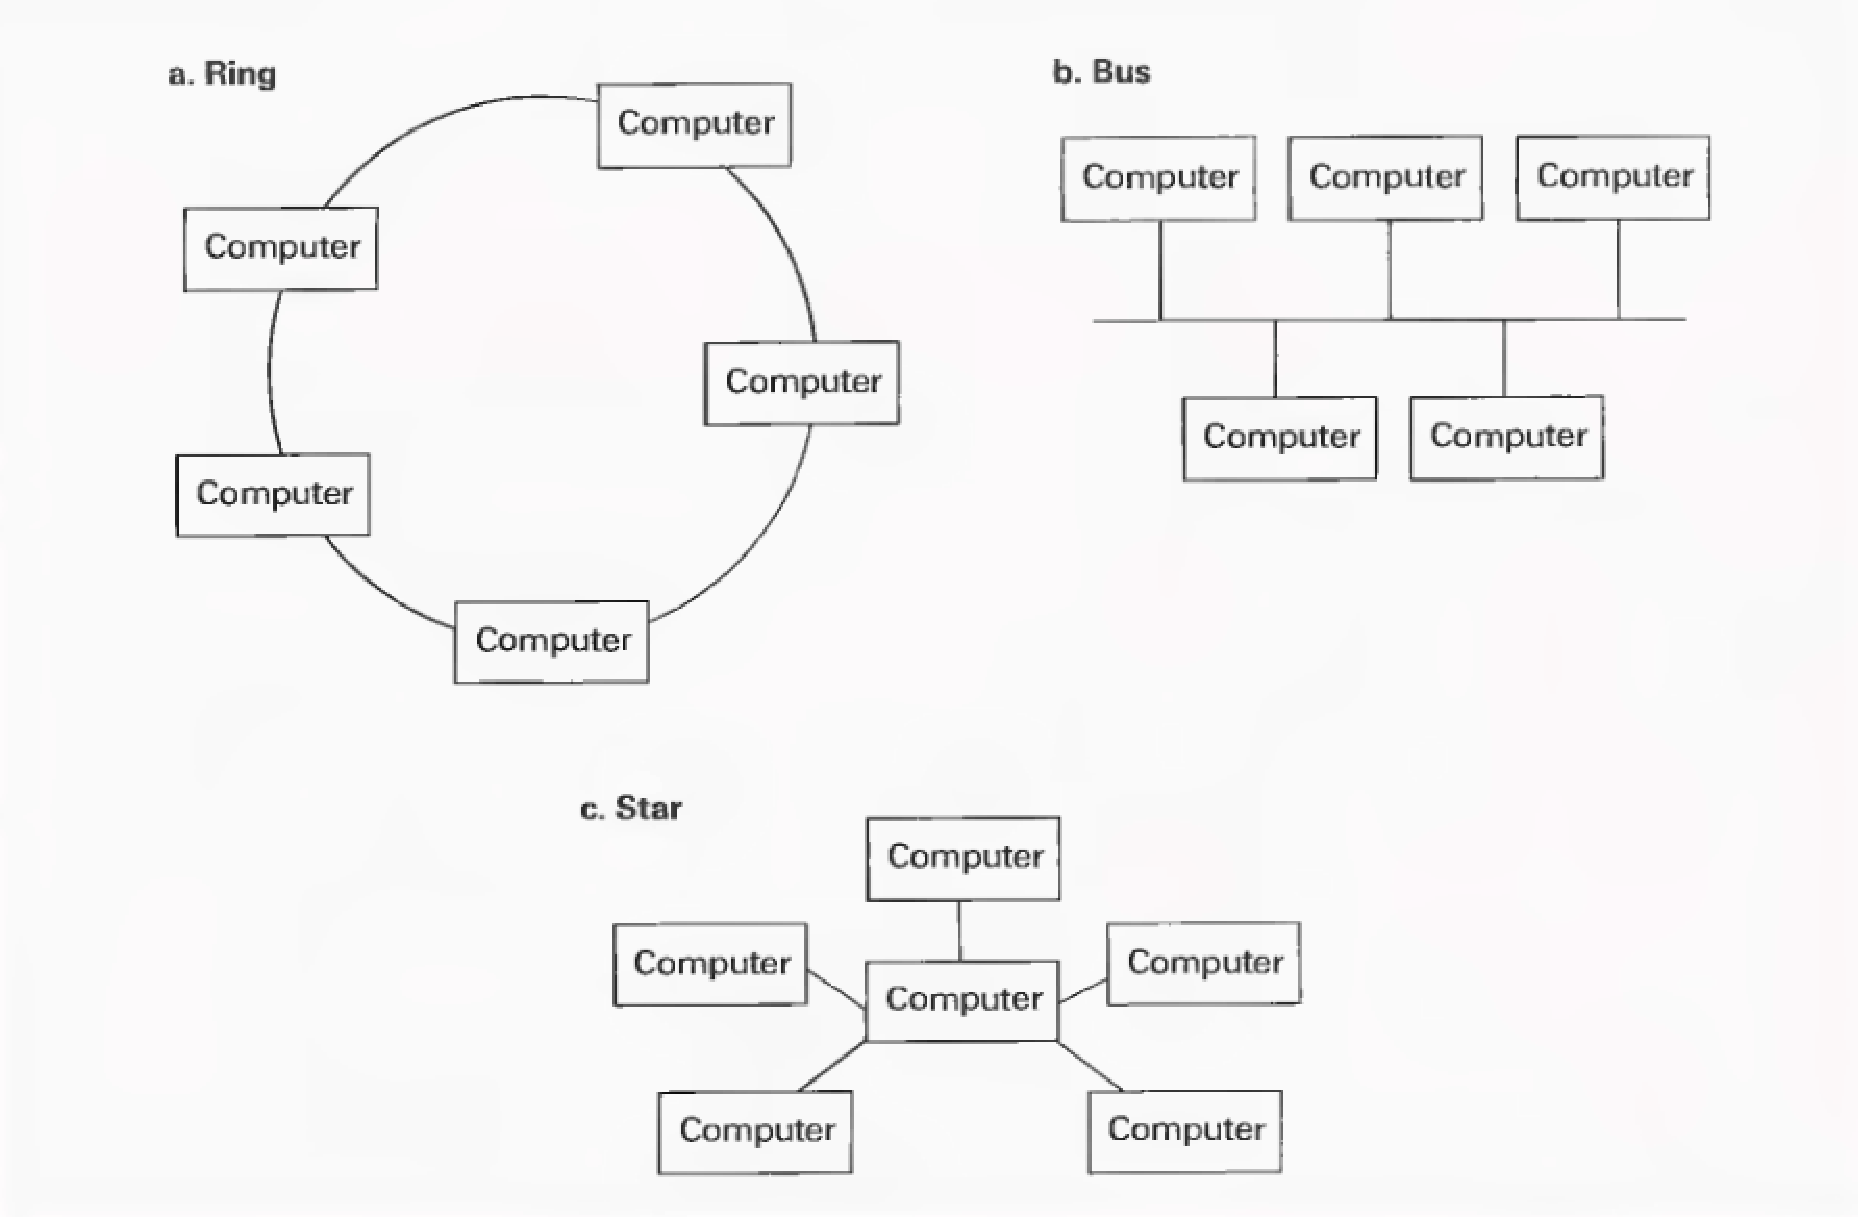
\includegraphics{ch5/fig41.pdf}}
\caption{Các hình trạng mạng}
  \label{fig:fig4.1}
\end{figure}

Còn một cách phân loại mạng khác đó là dựa trên hình trạng của mạng. Hình trạng mạng
là mô hình xác định cách để các thiết bị trong mạng kết nối với nhau. Hình~\ref{fig:fig4.1} giới
thiệu ba hình trạng mạng phổ biến:
\begin{inparaenum}[(1)]
\item Mạng vòng tròn (Ring), trong đó các thiết bị được kết nối với nhau
  theo hình tròn;
\item Mạng hình tuyến (Bus), trong đó tất cả các thiết bị được kết nối với nhau thông qua
  một đường truyền tải gọi là trục chính (Bus); và
\item Mạng hình sao, trong đó một thiết bị phục vụ như là một điểm trung tâm nơi mà các
  thiết bị khác được kết nối tới nó.
\end{inparaenum}

Trong những mô hình trên, mạng hình sao được sử dụng phổ biến nhất. Mạng này đã
phát triển từ mô hình trung tâm máy tính lớn phục vụ cho nhiều người sử dụng. Thể hiện rõ nhất là trường hợp những người dùng sử dụng các thiết bị đầu cuối kết nối vào các máy tính nhỏ. Ngày nay, mô hình mạng hình tuyến (bus) cũng
được sử dụng rộng rãi dưới hình thức mạng chuẩn là \textbf{Ethernet}, một
trong những mô hình mạng khá phổ biến.

Cần chú ý rằng hình trạng của mạng có thể không  thể hiện rõ qua mô hình vật
lý của nó. Ví dụ, một mạng hình tuyến (bus) không nhất thiết phải được triển khai
dưới một đường trục dài nơi mà các máy tính được kết nối thông qua các liên kết ngắn như
đã mô tả trong Hình~\ref{fig:fig4.1}. Thay vào đó, thông thường người ta dựng một mạng
hình tuyến bằng cách chạy các liên kết từ chính mỗi máy tính tới một vùng trung tâm, nơi
mà chúng được kết nối với nhau thông qua một thiết bị gọi là \textbf{hub}. Thiết bị hub
này nhỏ hơn bất kỳ một trục ngắn nào. Nó thực hiện tiếp sóng bất kỳ tín hiệu nào nó nhận
được (thông qua một vài bộ khuếch đại tín hiệu) và truyền tới tất cả các máy tính kết nối
với nó thông qua các cổng. Kết quả là một mạng trông như mạng hình sao lại được hoạt động
dưới hình thức là một mạng hình tuyến. Sự khác nhau ở đây là thiết bị trung tâm trong mô
hình mạng hình sao là một máy tính (thường là một thiết bị với nhiều khả năng hơn tại các
điểm nút của hình sao); nó  nhận và xử lý các thông điệp từ các máy tính khác. Ngược lại, thiết
bị trung tâm trong mô hình mạng hình tuyến là một hub; nó  chỉ đơn thuần cung cấp một kênh truyền
thông tin cho các máy tính.

Một quan điểm khác cũng cần phải chú ý là các kết nối giữa các thiết bị trong hệ thống
mạng không nhất thiết phải là các thiết bị vật lý. Hệ thống mạng không dây, sử dụng công
nghệ truyền phát qua sóng radio, cũng dần được sử dụng phổ biến. Đặc biệt, thiết bị hub
trong rất nhiều mô hình mạng hình tuyến ngày nay thực chất là một trạm tiếp và phát sóng
radio.

\subsection*{Các giao thức}
Để cho một hệ thống mạng hoạt động tin cậy, việc thiết lập những quy tắc nhờ
đó các hoạt động của mạng được kiểm soát là rất quan trọng. Những quy tắc này được gọi là
các \textbf{giao thức}. Thông qua việc phát triển và kế thừa các chuẩn giao thức, các nhà
cung cấp có thể xây dựng những sản phẩm cho các ứng dụng mạng tương thích với những sản
phẩm của nhà cung cấp khác. Việc phát triển các chuẩn giao thức là quá trình không
thể thiếu trong sự phát triển các công nghệ mạng.


Khi giới thiệu về khái niệm giao thức, ta hãy xem xét vấn đề  phối hợp truyền thông điệp giữa các máy tính trong một mạng. Nếu không có các quy tắc  quản lý quá
trình truyền  này, các máy tính có thể yêu cầu truyền thông điệp vào cùng một
thời điểm hoặc cũng có thể bị lỗi khi tiếp nhận các thông điệp khi hỗ trợ đó được yêu cầu.


\begin{figure}[tbh] 
\centering
    \scalebox{0.45}{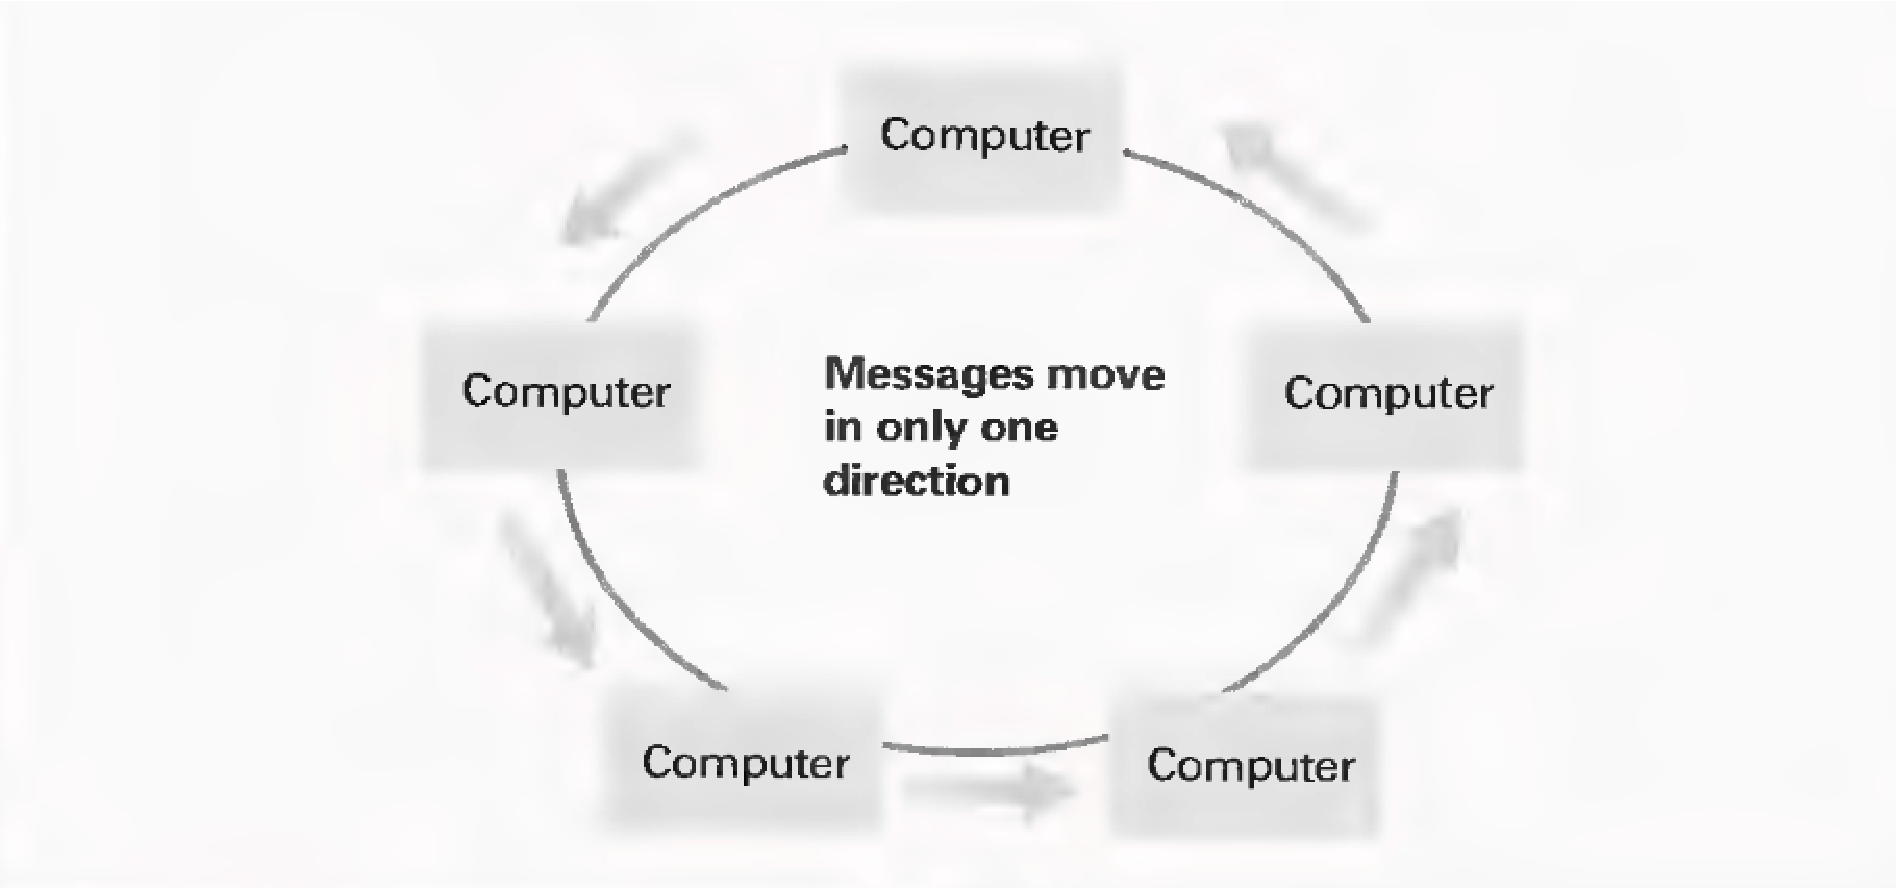
\includegraphics{ch5/fig42.pdf}}
    \caption{Truyền thông trong mạng vòng tròn}
  \label{fig:fig4.2}
\end{figure}

Một cách tiếp cận để có thể giải quyết được vấn đề này là giao thức \textbf{thẻ bài} trong
mạng vòng, được phát triển bởi IBM từ  những năm 1970 và tiếp tục trở nên phổ biến
trong các hệ thống mạng dựa trên nền tảng mô hình mạng vòng. Với giao thức này, tất
cả các thiết bị trong mạng truyền tải thông điệp theo một hướng chung duy nhất
(Hình~\ref{fig:fig4.2}), nghĩa là tất cả các thông điệp đó được gửi qua mạng di chuyển
vòng tròn theo cùng một hướng bằng cách chuyển tiếp từ máy tính này tới máy tính khác. Khi
một thông điệp được truyền tới đích của nó, máy tính đích giữ lại một bản sao và chuyển
tiếp một bản sao của thông điệp đó sang máy tính tiếp theo theo hình tròn. Khi bản sao
được chuyển tiếp về tới máy tính ban đầu, máy tính đó nhận thấy rằng thông điệp này đã
truyền được tới đích cần thiết, nó sẽ loại bỏ thông điệp ra khỏi vòng tròn. Tất nhiên, hệ
thống này còn phụ thuộc vào sự hợp tác của các liên máy tính. Nếu một máy tính yêu cầu
truyền phát liên tục các thông điệp từ chính nó thay vì chuyển tiếp các thông điệp sang
máy tính khác thì không có quá trình truyền tải nào được hoàn thành.


Để giải quyết vấn đề này, một xâu bít duy nhất, gọi là thẻ bài, được sử dụng trong quá
trình truyền tải theo vòng tròn. Quyền sở hữu của thẻ bài này được trao cho máy tính
nguồn, nơi bắt đầu truyền phát thông điệp; nếu không có thẻ bài, một máy tính chỉ được
phép chuyển tiếp thông điệp mà nó nhận được. Thông thường, mỗi máy tính đơn thuần chỉ tiếp
nhận và chuyển tiếp thẻ bài theo đúng cách mà nó chuyển tiếp thông điệp. Tuy nhiên, nếu
máy tính nhận được thẻ bài có thông điệp của chính nó đưa lên mạng, nó sẽ truyền một thông
điệp trong khi giữ lại thẻ bài. Khi thông điệp này hoàn tất quá trình truyền tải qua một
vòng tròn, máy tính chuyển tiếp thẻ bài cho máy tính tiếp theo trong vòng tròn. Như vậy,
khi máy tính tiếp theo nhận được thẻ bài, nó có thể chuyển tiếp thẻ bài ngay lập tức hoặc
truyền phát một thông điệp mới của mình trước khi chuyển tiếp thẻ bài cho máy tính tiếp
theo. Theo cách thức này, mỗi máy tính trong mạng đều có cơ hội như nhau để có thể gửi
thông điệp của nó cũng như thẻ bài đi xung quanh vòng tròn.


\begin{figure}[tbh]
\centering
    \scalebox{0.4}{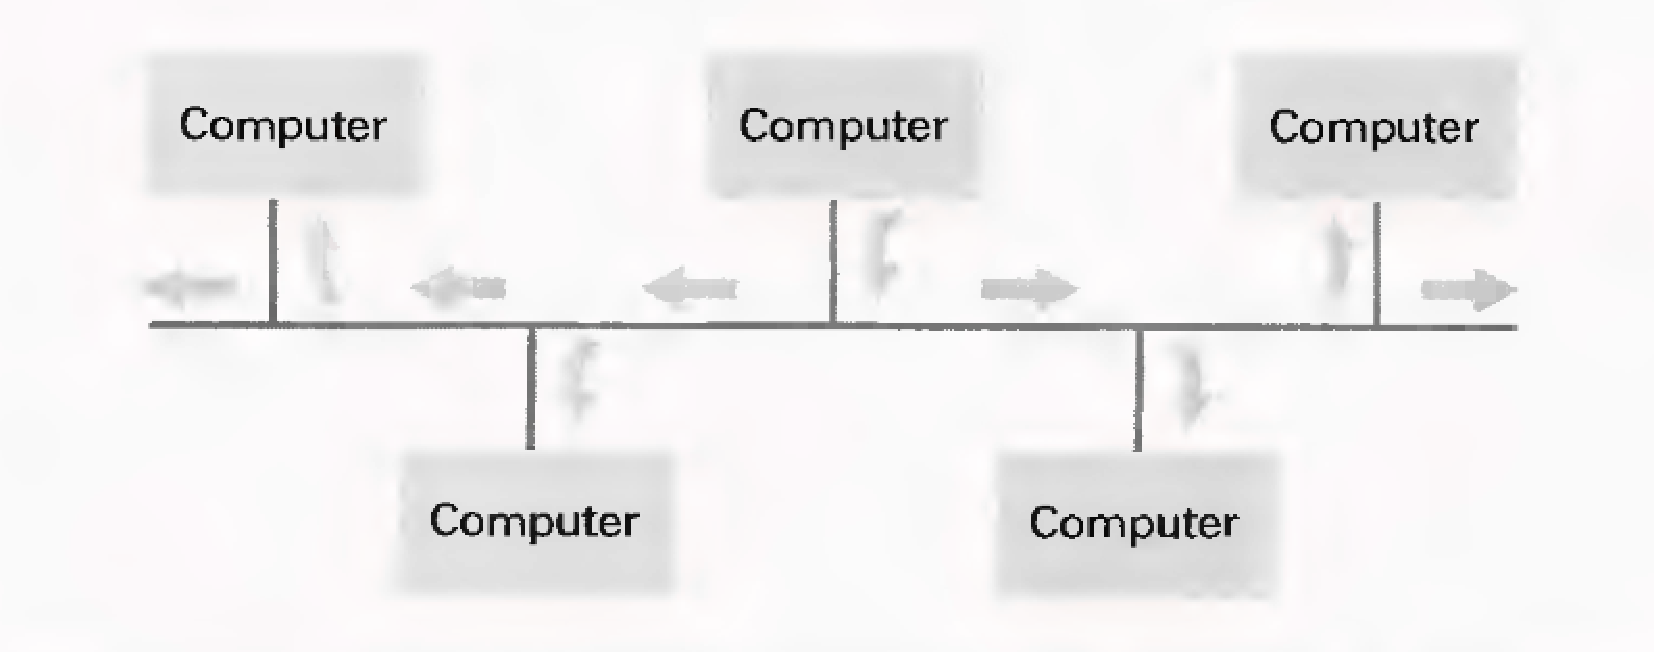
\includegraphics{ch5/fig43.pdf}}
    \caption{Truyền thông trong mạng hình tuyến}
  \label{fig:fig4.3}
\end{figure}

Một giao thức khác cũng được sử dụng trong công nghệ mạng hình tuyến cho việc phối hợp
truyền tải các thông điệp, đó là giao thức dựa trên tập các giao thức Ethernet. Trong hệ
thống mạng Ethernet, quyền truyền tải thông điệp được điều khiển bởi giao thức \textbf{Đa
  truy nhập có thăm dò và tách đụng độ} (Carrier Sense, Multiple Access with Collision
Detection--CSMA/CD). Giao thức này yêu cầu mỗi thông điệp phải được quảng bá cho tất cả
các máy tính trong trục chính (Hình~\ref{fig:fig4.3}). Mỗi máy tính sẽ theo dõi tất cả các
thông điệp những chỉ giữ lại những thông điệp nào được gửi tới chính nó thông qua địa
chỉ. Để truyền phát một thông điệp, một máy tính đợi cho đến khi đường trục chính rỗi, và
tại thời điểm này nó sẽ bắt đầu truyền phát tín hiệu trong khi tiếp tục theo dõi đường
trục chính. Nếu một máy tính khác cũng bắt đầu truyền tín hiệu, cả hai máy tính sẽ phát
hiện ra sự xung đột và sẽ tạm dừng trong một khoảng thời gian ngẫu nhiên trước khi truyền
tín hiệu lại. Một nhóm nhỏ người có nhu cầu đàm luận với nhau có thể sử dụng một hệ thống
tương đương như vậy. Nếu hai người cùng bắt đầu nói tại một thời điểm, cả hai sẽ dừng
lại. Một trong hai người có thể sẽ tiếp tục với một chuỗi câu như ``Xin lỗi, anh định nói
gì vậy?'', ``Không, không. Anh nói trước đi'', trong khi với giao thức CSMA/CD, mỗi máy
tính đơn thuần chỉ là thử truyền phát tín hiệu lại.


\subsection*{Kết hợp các hệ thống mạng}

Đôi khi cần phải kết nối các hệ thống mạng đã tồn tại thành một hệ thống truyền thông mở
rộng. Điều này có thể được thực hiện bằng việc kết nối các mạng thành một phiên bản lớn
hơn nhưng vẫn cùng ``kiểu'' như hệ thống cũ. Ví dụ, trong trường hợp những hệ thống mạng
hình tuyến dựa trên các giao thức mạng Ethernet, thông thường có thể kết nối các trục
chính thành một trục đơn lớn hơn. Việc này được thực hiện với điều kiện sử dụng các thiết
bị khác nhau được biết đến như\textbf{ bộ lặp tín hiệu} (repeater), \textbf{cầu nối}
(bridge), và \textbf{bộ chuyển mạch} (switch), đó là những sự khác biệt không dễ phát hiện
ra nhằm phục vụ cho việc mở rộng hệ thống mạng. Đơn giản nhất trong số đó là bộ lặp tín
hiệu, thiết bị dùng để kết nối trục chính của hai mạng hình tuyến lại với nhau thành một
trục dài hơn (Hình~\ref{fig:fig4.4}). Bộ khuếch đại (bộ lặp tín hiệu) đơn giản chỉ truyền
các tín hiệu về phía sau hay trước giữa hai tuyến gốc ban đầu (thông thường sử dụng với
một vài bộ khuếch đại tín hiệu) mà không cần biết ý nghĩa của những tín hiệu đó là gì.

\begin{figure}[tb] 
  \centering \scalebox{0.45}{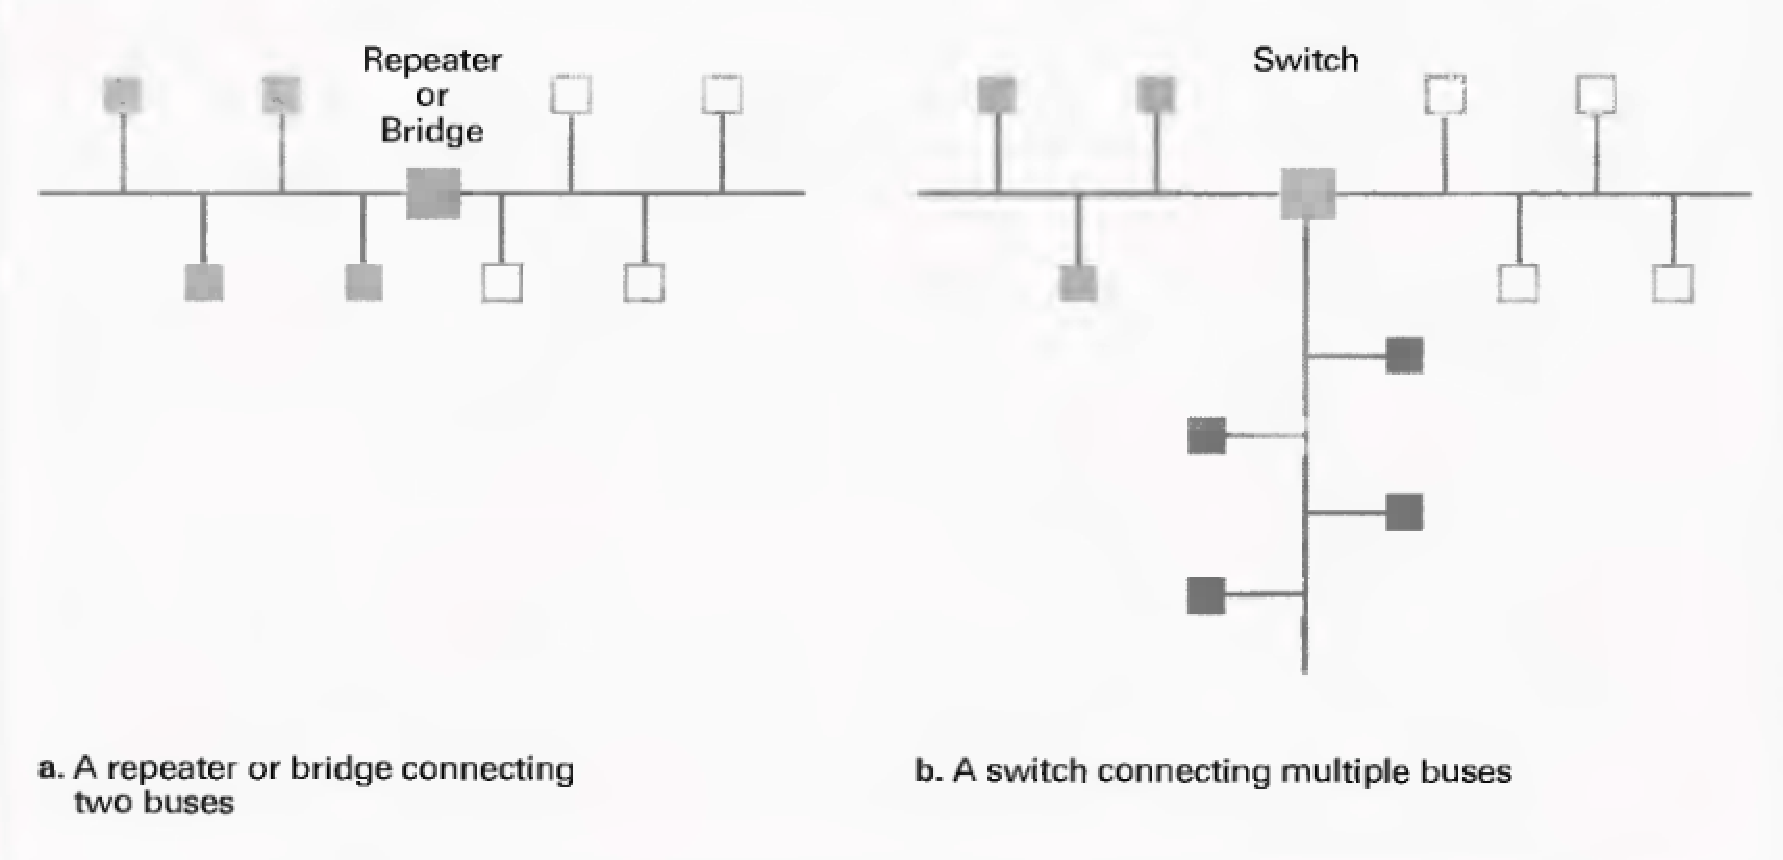
\includegraphics{ch5/fig44.pdf}}
  \caption{Xây dựng một mạng hình tuyến lớn từ những mạng nhỏ hơn}
  \label{fig:fig4.4}
\end{figure}

\textbf{Cầu nối} là một thiết bị tương đương, nhưng phức tạp hơn so với bộ lặp tín
hiệu. Cũng như bộ lặp tín hiệu, cầu nối kết nối hai mạng hình tuyến với nhau, nhưng nó
không nhất thiết phải chuyển tiếp tất cả các thông điệp từ tuyến này sang tuyến kia. Thay
vào đó, nó sẽ xem địa chỉ đích đi kèm với thông điệp và chuyển tiếp thông điệp qua kết nối
chỉ khi thông điệp đó đã được chỉ định trước là sẽ được gửi tới một máy tính ở phía bên
kia của kết nối. Do đó, hai thiết bị nằm ở trên cùng một phía của cầu nối có thể trao đổi
thông điệp mà không gây phiền phức cho sự truyền thông ở phía bên kia của cầu. Cầu nối
thường làm việc có hiệu quả hơn so với bộ lặp tín hiệu.

\textbf{Bộ chuyển mạch} về bản chất là một cầu nối có nhiều cổng kết nối, cho phép nó kết
nối tới nhiều hơn hai tuyến. Do đó, bộ chuyển mạch tạo ra một mạng bao gồm một vài tuyến
được mở rộng từ bộ chuyển mạch như những chiếc nan hoa của bánh xe
(Hình~\ref{fig:fig4.4}b). Cũng giống như cầu nối, bộ chuyển mạch sẽ xem xét địa chỉ đích
của tất cả các thông điệp và chỉ chuyển tiếp những thông điệp nào đã được chỉ định trước
sang các tuyến khác. Hơn nữa, mỗi thông điệp được chuyển tiếp chỉ được chuyển tới các
tuyến tương ứng của địa chỉ đích, chính vì vậy mà nó có thể giảm thiểu được giao thông
trên mỗi tuyến.

Cần phải chú ý rằng khi các mạng được kết nối với những thiết bị như bộ lặp tín hiệu, cầu
nối hay thiết bị chuyển mạch, kết quả là một mạng đơn lớn hơn được tạo ra. Mỗi máy tính
tiếp tục truyền tải thông qua hệ thống theo cách thức cũ (sử dụng cùng một giao thức mạng)
nếu hệ thống được xây dựng ban đầu như là một mạng đơn lớn. Điều đó có nghĩa là, các máy
tính cá nhân trong hệ thống không cần biết đến sự tồn tại của các bộ lặp tín hiệu, các cầu
nối, hay các thiết bị chuyển mạch.

Tuy nhiên, các hệ thống mạng được kết nối đôi khi cũng có những đặc tính không tương thích
nhau. Ví dụ, những đặc tính của mạng vòng tròn sử dụng giao thức thẻ bài vòng tròn
không tương thích với mạng Ethernet hình tuyến sử dụng CSMA/CD. Trong những trường hợp
này, các hệ thống mạng cần phải được kết nối theo một cách thức dùng để tạo ra hệ thống
mạng của các mạng, được biết đến như là hệ thống \textbf{liên mạng} (internet), trong đó
những mạng gốc ban đầu duy trì những tính chất riêng của chúng và tiếp tục vận hành như là
những hệ thống độc lập. (Chú ý rằng \textit{liên mạng (internet)} khác với mạng
\textit{Internet}. Mạng Internet, với chữ cái I được viết hoa, được nói đến như một hệ
thống liên mạng đặc biệt, có phạm vi rộng lớn mà ta sẽ nghiên cứu trong một phần khác của
chương này. Có rất nhiều ví dụ về những hệ thống liên mạng. Quả thực, hệ thống truyền
thông qua điện thoại cổ điển đã được sử dụng khá tốt trong các hệ thống liên mạng phạm vi
rộng trước khi mà mạng Internet được phổ biến.)


\begin{figure}[tb] 
  \centering \scalebox{0.45}{\includegraphics{ch5/fig45.pdf}}
  \caption{Bộ dẫn đường kết nối một mạng hình tuyến với một mạng hình sao tạo thành một hệ
    thống liên mạng}
  \label{fig:fig4.5}
\end{figure}

Sự kết nối giữa hai hệ thống mạng tạo thành một hệ thống liên mạng được thực hiện bởi một
thiết bị gọi là \textbf{bộ dẫn đường} (Router). Một bộ dẫn đường là một máy tính thuộc về
cả hai hệ thống mạng ở hai phía của nó với nhiệm vụ là chuyển tiếp các thông điệp từ mạng
này sang mạng kia (Hình~\ref{fig:fig4.5}). Chú ý rằng nhiệm vụ của bộ dẫn đường đặc biệt
to tát hơn nhiều so với các thiết bị như bộ lặp tín hiệu, cầu nối hay thiết bị chuyển mạch
bởi vì một bộ dẫn đường cần phải thực hiện chuyển đổi giữa các đặc tính riêng biệt của hai
mạng gốc ban đầu. Ví dụ, khi truyền phát một thông điệp từ một mạng sử dụng giao thức thẻ
bài vòng tròn tới một mạng sử dụng giao thức CSMA/CD, bộ dẫn đường phải nhận thông điệp sử
dụng một giao thức sau đó lại sử dụng một giao thức khác để truyền thông điệp đó tới mạng
kia.


Ta sẽ xem xét một ví dụ khác sẽ mô tả sự phức tạp khi thực hiện việc dẫn đường của
Router. Đó là vấn đề khi hai mạng kết nối với nhau lại sử dụng hai hệ thống địa chỉ khác
nhau để xác định các máy tính trong mạng. Khi một máy tính trong một mạng muốn gửi một
thông điệp tới một máy tính ở mạng bên kia, nó không thể xác định được máy tính đích theo
cách thức thông thường mà nó vẫn thường thực hiện.

\begin{figure}[t]
  \begin{quotation}
    \noindent
    \textbf{Mạng Enthernet} \vspace{0.3cm}
    \\
    Mạng Ethernet là một tập các chuẩn được triển khai trong một mạng LAN với mô hình mạng
    hình tuyến. Tên gọi của nó được bắt nguồn từ thiết kế mạng Ethernet ban đầu trong đó
    các thiết bị được kết nối với nhau qua cáp đồng trục. Khởi đầu mạng Ethernet được phát
    triển vào những năm 1970 và ngày nay được chuẩn hóa bởi IEEE là một phần của họ chuẩn
    IEEE 802, mạng Ethernet có hầu hết các cách thức chung của một mạng các máy tính. Việc
    cài đặt các card điều khiển mạng của các máy tính cá nhân trong mạng Ethernet có thể
    thực hiện được và khá dễ dàng.

    Ngày nay trên thực tế có một vài phiên bản của mạng Ethernet với những công nghệ tiên
    tiến hơn và tốc độ truyền tải thông tin cũng cao hơn. Tuy nhiên, tất cả những phiên
    bản mới đó vẫn có đủ các đặc tính chung của họ mạng Ethernet. Mỗi một phiên bản trong
    số đó là một khuôn thức mà trong đó dữ liệu được đóng gói trước khi truyền đi, sử dụng
    mã hóa Manchester (một phương pháp mà trong đó đại diện là các bít 0 và 1, với một bít
    0 sẽ đại diện cho một tín hiệu giảm dần và bít 1 đại diện cho một tín hiệu tăng dần)
    để truyền tải thực sự các bít dữ liệu, và sử dụng giao thức CSMA/CD để điều khiển
    quyền truyền phát.
  \end{quotation}
\end{figure}

Trong những trường hợp như vậy, một hệ thống địa chỉ với phạm vi liên mạng được thiết
lập. Kết quả là mỗi thiết bị trong một hệ thống liên mạng có hai địa chỉ: một địa chỉ của
chính mạng gốc ban đầu của nó và một địa chỉ liên mạng mới. Để gửi một thông điệp từ một
máy tính thuộc một trong những mạng gốc tới một máy tính trong mạng khác--máy tính có địa chỉ
liên mạng của gói tin gốc ban đầu, nó sẽ sử dụng hệ thống địa chỉ gốc của mạng cục bộ để
gửi gói tin tới bộ dẫn đường. Bộ dẫn đường sau đó sẽ xem xét bên trong của gói tin nhận
được, thực hiện tìm địa chỉ liên mạng đích sau cùng của thông điệp, dịch địa chỉ đó thành
địa chỉ có định dạng thích hợp với mạng kia, sau đó chuyển tiếp thông điệp tới đích của
nó. Nói một cách ngắn gọn, các thông điệp trong mỗi một mạng gốc tiếp tục được truyền theo
cách thức của hệ thống địa chỉ gốc của mỗi mạng, và bộ dẫn đường được phân công nhiệm vụ
là chuyển đổi giữa các hệ thống.

\subsection*{Truyền thông liên tiến trình}
Các tiến trình thực thi trên các máy tính khác nhau trong một mạng
máy tính (hay thậm chí trên cùng một máy  theo cách thức chia sẻ thời gian)
thường phải liên lạc với các tiến trình khác  để thực hiện những nhiệm vụ đã được xác định. Việc liên lạc này được gọi là sự \textbf{truyền thông liên tiến trình}.

Một trong những phương thức phổ biến trong truyền thông liên tiến trình là mô hình
\textbf{khách/chủ} (client/server). Mô hình này xác định  vai trò của các tiến
trình trên máy trạm, nơi mà sẽ phát sinh các yêu cầu tới các tiến trình khác trên máy chủ, và các tiến trính trên máy chủ  
nơi sẽ thực hiện các yêu cầu của máy trạm.

Một ứng dụng sơ khai trong mô hình khách/chủ đã xuất hiện trên những mạng liên kết tất cả
máy tính trong một nhóm các văn phòng. Trong tình huống như vậy, một máy in đơn lẻ, chất
lượng cao được kết nối vào mạng nơi mà tất cả các máy tính trong đó có thể sử dụng được
máy in đó. Với trường hợp này máy in đã đóng vai trò của một máy chủ (thường được gọi là
\textbf{máy chủ in} (printer server), và các máy tính khác được lập trình để đóng vai của
các máy trạm sẽ gửi các yêu cầu in ấn tới máy chủ in.

Một ứng dụng khác của mô hình khách/chủ cũng sớm được đưa vào sử dụng nhằm giảm chi phí
lưu trữ bằng cách loại bỏ những nhu cầu về các bản sao trùng lặp của những mẫu tin. Ở đây,
một máy tính trong mạng được trang bị một hệ thống lưu trữ thứ cấp có khả năng cao (thường
sử dụng một đĩa từ) mà trên đó chứa toàn bộ các thông tin dữ liệu của một đơn vị. Các máy
tính khác trên mạng có thể yêu cầu truy cập tới các thông tin dữ liệu mà chúng cần. Khi
đó, máy tính chứa thông tin dữ liệu đóng vai trò là một máy chủ (gọi là \textbf{máy chủ
  file}--file server), và các máy tính khác đóng vai trò là các máy trạm sẽ gửi các yêu
cầu truy cập với những file dữ liệu được lưu trữ trên máy chủ file.

\begin{figure}[tb] 
  \centering \scalebox{0.4}{\includegraphics{ch5/fig46.pdf}}
  \caption{Mô hình client/server so sánh với mô hình peer-to-peer}
  \label{fig:fig4.6}
\end{figure}

Ngày nay, mô hình khách/chủ được sử dụng rộng rãi trong các ứng dụng mạng, ta sẽ xem xét ở
phần sau trong chương này. Tuy nhiên, không chỉ mô hình khách/chủ mới hoạt động theo cách
thức như một sự truyền thông liên tiến trình. Một mô hình khác với tên gọi
\textbf{peer-to-peer} (thường được viết tắt là P2P), có những tính chất trái ngược hoàn
toàn với mô hình khách/chủ. Trong khi mô hình khách/chủ bao gồm một tiến trình (trên máy
chủ) thực hiện liên lạc với nhiều tiến trình khác (tại các máy trạm) thì mô hình
peer-to-peer lại bao gồm hai tiến trình trao đổi ngang hàng với nhau
(Hình~\ref{fig:fig4.6}). Ngoài ra, một máy chủ phải chạy liên tục nhằm phục vụ cho các máy
trạm của nó tại bất kỳ thời điểm nào, ngược lại mô hình peer-to-peer với hai tiến trình có
thể thực hiện theo cách thức tạm thời. Ví dụ, các ứng dụng trong mô hình peer-to-peer bao
gồm việc gửi tức thì các thông điệp mà hai người thực hiện đối thoại với nhau qua Internet
cũng như những tình huống như hai người chơi những trò chơi như cờ vua hay cờ đam (một
loại trò chơi gồm 24 quân cờ cho 2 người chơi).


Mô hình peer-to-peer cũng hoạt động theo cách thức chia sẻ file như các bản nhạc hay những
bộ phim qua Internet (đôi khi đi kèm là vấn đề về bản quyền). Trong trường hợp này, những
cá nhân cần tìm kiếm những khoản mục phổ biến có thể quảng bá mong muốn của họ lên
Internet và liên hệ được với những ai sở hữu những khoản mục đó. Sau đó, những khoản mục
này được truyền tải giữa hai phía sử dụng mô hình peer-to-peer. Điều này trái ngược hoàn
toàn với cách tiếp cận của mô hình khách/chủ qua việc thiết lập một ``trung tâm phân
phối'' (máy chủ file) cho các máy trạm tải các bản nhạc (hay ít nhất là tìm thấy các nguồn
của những khoản mục đó). Tuy nhiên, máy chủ trung tâm, đã chứng thực được là một điểm
trung tâm mà tại đó ngành công nghiệp âm nhạc có thể được tuân thủ theo đúng luật bản
quyền, dẫn tới kết quả cuối cùng là sự dỡ bỏ các trung tâm phân phối âm nhạc. Ngược lại,
sự thiếu vắng các trung tâm điều hành như vậy trong mô hình peer-to-peer sẽ khiến nỗ lực
làm cho luật bản quyền có hiệu lực trở nên khó khăn.

Thông thường bạn có thể đọc và nghe về \textit{mạng peer-to-peer}, ví dụ như việc sử dụng
sai những thuật ngữ có thể mắc phải khi những ngôn từ kỹ thuật được thông qua bởi một cộng
đồng phi kỹ thuật. Mạng \textit{peer-to-peer} được biết đến như một hệ thống mà trong đó,
hai tiến trình trao đổi với nhau qua mạng (hoặc liên mạng). Nó không phải là một thuộc
tính của mạng (hay liên mạng). Một tiến trình có thể sử dụng mô hình peer-to-peer để trao
đổi với tiến trình khác thông qua cùng một hệ thống mạng. Vì vậy cần phải nói một cách
chính xác là truyền thông theo cách thức của mô hình peer-to-peer chứ không phải là truyền
thông qua một mạng peer-to-peer.

\subsection*{Các hệ thống phân tán}
Với sự thành công của công nghệ mạng, sự tương tác giữa những máy tính qua các hệ thống
mạng trở nên phổ biến và được thể hiện ở nhiều khía cạnh. Nhiều hệ thống phần mềm hiện
đại, như các hệ thống tìm kiếm hay phục hồi thông tin toàn cầu, các hệ thống kiểm toán có
phạm vi toàn công ty, các trò chơi máy tính, và thậm chí các phần mềm điều khiển chính hệ
thống cơ sở hạ tầng của mạng được thiết kế như là những \textbf{hệ thống phân tán}. Điều
đó có nghĩa là chúng gồm có những đơn vị phần mềm được thực thi dưới dạng các tiến trình trên
các máy tính khác nhau. Ta có thể hình dùng những tiến trình này như là những vị khách cư
trú tại các máy tính khác nhau mà qua đó các máy tính trong một mạng sẽ được gọi là các
\textbf{máy chủ} (host). Điều đó có nghĩa rằng host là một máy tính mà các tiến trình
trú ngụ trên đó theo một hay nhiều ngữ cảnh.

Các hệ thống phân tán đầu tiên được phát triển độc lập từ những hệ thống hỗn tạp. Nhưng
ngày nay, việc nghiên cứu một cách cẩn thận đã cho thấy một cơ sở hạ tầng phổ biến vận
hành trong suốt toàn bộ những hệ thống này, bao gồm cả những thứ như các hệ thống truyền
thông và bảo mật. Đổi lại, kết quả của sự cố gắng đã tạo ra các hệ thống mà có thể cung
cấp cơ sở hạ tầng cơ bản và chính vì vậy, nó cho phép các ứng dụng phân tán được xây dựng
bởi sự phát triển phần hệ thống duy nhất đối với ứng dụng đó.

Một kết quả của nhận định trên là hệ thống đặc tả về giao diện lập trình JavaBeans (được
phát triển bởi Sun Microsystems). Hệ thống này là một môi trường phát triển trợ giúp việc
xây dựng các hệ thống phần mềm phân tán mới. Sử dụng JavaBeans, một hệ thống phân tán được
xây dựng từ những đơn vị được gọi là các bean được tự động thừa kế những đặc tính cơ sở hạ
tầng của hệ thống cha. Do đó, chỉ có những thành phần ứng dụng phụ thuộc duy nhất của một
hệ thống mới mới được phát triển. Một cách tiếp cận khác là môi trường phát triển phần mềm
với tên gọi .NET Framework (được phát triển bởi Microsoft). Với thuật ngữ .NET, các thành
phần của hệ thống phân tán được gọi là các assembly. Mặt khác, bằng việc phát triển các
đơn vị này trong môi trường .NET, chỉ những nét đặc trưng duy nhất đối với một ứng dụng
phổ biến là cần phải được xây dựng dựa trên nền tảng cơ sở hạ tầng có sẵn. Cả hai môi
trường JavaBeans và .NET Framework đều rất đơn giản trong việc phát triển các hệ thống
phần mềm phân tán mới.

\subsection*{Câu hỏi \& Bài tập}

\begin{enumerate}
\item Thế nào là một hệ thống mạng mở?

\item Tóm tắt những đặc tính khác biệt giữa thiết bị lặp tín hiệu và cầu nối

\item Thiết bị dẫn đường là gì?

\item Mô tả một vài mối quan hệ trong xã hội tuân theo mô hình khách/chủ.

\item Mô tả một vài giao thức được sử dụng trong xã hội.

\end{enumerate}



%%% Local Variables: 
%%% mode: latex
%%% TeX-master: "../tindaicuong"
%%% End: 


\section{Mạng Internet}
\label{sec:4.2}
Một trong những hệ thống liên mạng nổi trội nhất đó là mạng \textbf{Internet} (chú ý chữ I
viết hoa), đây là hệ thống mà bắt nguồn từ những dự án nghiên cứu từ những năm 1960 trở về
trước. Mục đích là phát triển khả năng kết nối nhiều mạng máy tính mà chúng có chức năng
như là một hệ thống kết nối không bị phá vỡ bởi những nguy cơ cục bộ. Hầu hết những công
việc ban đầu đều được tài trợ bởi chính phủ Mỹ thông qua Quỹ nghiên cứu Bộ quốc phòng Mỹ
(DARPA - được phát âm là ``DAR-pa''). Trải qua nhiều năm, sự phát triển của mạng Internet
thay đổi (thăng trầm) từ dự án quốc phòng tới dự án nghiên cứu mang tính chất học thuật,
và ngày nay nó được coi là một hệ thống thương mại mà có thể nối kết một tổ hợp các mạng
WAN, MAN, và LAN bao gồm hàng triệu máy tính.

\subsection*{Cấu trúc mạng Internet}
Về khía cạnh khái niệm, mạng Internet có thể được xem như là một tập hợp nhiều
\textbf{miền} (domains), mỗi miền bao gồm một mạng máy tính hay một liên mạng vừa và nhỏ được
điều hành bởi một tổ chức độc lập như một trường đại học, một công ty, hay cơ quan thuộc
chính phủ. Mỗi miền là một hệ thống tự trị (autonomous system) mà có thể được cấu hình với
yêu cầu về mức độ quyền hạn cục bộ. Nó có thể bao gồm một máy tính đơn hay một hệ thống
liên mạng phức tạp có thể bao gồm rất nhiều mạng LAN, MAN, hay thậm chí là mạng WAN.

Sự thành lập của các miền được giám sát bởi \textbf{ICANN (Internet Corporation for
  Assigned Names and Numbers)}, là một tổ chức phi lợi nhuận thực hiện việc thiết lập tên
cho các miền và gán các địa chỉ Internet, ta sẽ xem xét tới vấn đề này ngay sau
đây. Để thành lập một miền trên mạng Internet, miền đó trước tiên phải được đăng ký thông
qua các công ty, gọi là các nhà đăng ký mà đại diện cho tổ chức ICANN.


\begin{figure}[t]
  \begin{quotation}
    \noindent
    \textbf{Internet2} \vspace{0.3cm}
    \\
    Ngày nay mạng Internet đã thay đổi từ một dự án nghiên cứu thành một sản phẩm mang
    tính chất gia đình, cộng đồng nghiên cứu đã chuyển sang một dự án mang tên
    Internet2. Internet2 được mong đợi như là một hệ thống có tính chất học thuật và bao
    gồm rất nhiều các trường đại học làm việc công tác với ngày công nghiệp và chính
    phủ. Mục đích là kiểm soát việc nghiên cứu đối với các ứng dụng liên mạng yêu cầu độ
    rộng dải tần cao trong truyền thông, như hệ thống truy cập và điều khiển từ xa của
    những thiết bị đắt tiền như kính viễn vọng và những thiết bị chẩn đoán trong y tế. Một
    ví dụ của nghiên cứu này là việc thực hiện phẫu thuật từ xa thông qua bàn tay của rô
    bốt bắt chước các cử động của đôi bàn tay của một nhà phẫu thuật ngồi từ xa và quan
    sát bệnh nhân qua băng video. Bạn có thể xem thêm về Internet2 tại địa chỉ \url{
      http://www.internet2.org}
  \end{quotation}
\end{figure}


Khi một miền được đăng ký, nó có thể được gắn vào mạng Internet hiện tại thông qua một bộ
dẫn đường (router) mà kết nối một trong những mạng trong miền tới một mạng đã tồn tại trên
Internet. Bộ dẫn đường đặc biệt này thường được xem như là một cổng vào/ra (gateway) của
miền mà qua đó, nó đại diện cho cổng của miền ra phần còn lại của Internet. Xét trên góc
độ tầm nhìn, nó là một miền đơn lẻ, phần mạng của Internet nằm phía ngoài của cổng vào ra đôi
khi được gọi là đám mây (cloud).

\subsection*{Kết nối tới mạng Internet}

Để đơn giản hóa quá trình kết nối tới mạng Internet, rất nhiều công ty, được gọi là
\textbf{nhà cung cấp dịch vụ Internet (ISP)}, cho phép các khách hàng kết nối những miền
của họ ra ngoài Internet thông qua các thiết bị của ISP hay trở thành một phần của một
miền đã được thiết lập bởi ISP. Có lẽ những cách thức kết nối với chi phí ít tốn kém nhất
tới một ISP vẫn được sử dụng là thông qua các kết nối điện thoại được gọi là kết nối kiểu
quay số (dial-up). Bằng việc sử dụng theo cách thức này, một cá nhân có thể kết nối máy
tính của anh ta hay của cô ta tới đường thoại cục bộ và thực thi một gói phần mềm với
nhiệm vụ gọi đến một máy tính đặt tại ISP. Tại thời điểm đó, ISP cung cấp truy cập
Internet trong suốt thời gian gọi của điện thoại.


\begin{figure}[bth] 
  \centering \scalebox{0.45}{\includegraphics{ch5/fig47.pdf}}
  \caption{ Một cách thức kết nối điển hình tới mạng Internet}
  \label{fig:fig4.7}
\end{figure}

\subsection*{Đánh địa chỉ Internet}
Như đã giới thiệu trong Mục~\ref{sec:4.1}, một liên mạng cần phải được kết hợp với một hệ
thống địa chỉ liên mạng diện rộng mà sẽ gán một địa chỉ xác định cho mỗi máy tính trong hệ
thống. Trong Internet, những địa chỉ này được biết đến như là những \textbf{địa chỉ IP}
(Ký hiệu IP được viết tắt từ cụm “Internet Protocol”, khái niệm mà ta sẽ được giới thiệu
trong Mục~\ref{sec:4.4}). Mỗi địa chỉ IP là một bộ gồm 32 bít và trên thực tế cho đến ngày
nay địa chỉ IP đang trên đà tăng lên thành 128 bít (xem thảo luận về IPv6 trong phần
4.4). Mỗi địa chỉ 32 bít bao gồm hai phần: một phần xác định miền mà trong đó các máy tính
cư trú và một phần xác định mỗi máy tính cụ thể trong miền đó. Phần địa chỉ xác định miền,
được gọi là phần \textbf{định danh mạng}, được gán dưới sự kiểm soát của ICANN tại thời
điểm mà miền đó được đăng ký. Như vậy thông qua quá trình đăng ký này mà mỗi miền trong
mạng Internet được đảm bảo chắc chắn là có một định danh mạng là duy nhất. Phần địa chỉ
xác định một máy tính cụ thể trong miền được gọi là \textbf{địa chỉ máy chủ} (host). Địa
chỉ host được gán bởi người có thẩm quyền trong nội bộ miền đó, thông thường là người có
công việc như quản trị mạng hay quản trị hệ thống.

Địa chỉ IP theo truyền thống được viết thông qua các \textbf{dấu chấm thập phân} ngăn cách
các byte của địa chỉ mà được phân chia theo đoạn và mỗi byte được biểu diễn dưới dạng là
một số nguyên ở dạng thập phân. Ví dụ, sử dụng dấu chấm thập phân, chuỗi 5.2 sẽ được phân
tách thành một chuỗi bít hai byte $0000010100000010$, trong đó bao gồm byte $00000101$
(đại diện cho $5$) và byte liền sau đó là byte $00000010$ (đại diện cho $2$), và chuỗi
$17.12.25$ được biểu diễn thành một chuỗi bít ba byte bao gồm byte $00010001$ (là số $17$
được viết dưới dạng nhị phân), byte sau đó là byte $00001100$ (là số $12$ được viết dưới
dạng nhị phân), và byte cuối cùng là byte $00011001$ (là số $25$ được viết dưới dạng nhị
phân). Như vậy, một máy tính trong miền của Nhà xuất bản~Addison-Wesley có thể có địa chỉ
là $192.207.177.133$, trong đó ba byte đầu tiên ($192.207.177$) được hiểu là định danh cho
mạng (xác định miền Addison-Wesley) và byte cuối cùng ($133$) là địa chỉ host (xác định
một máy tính cụ thể trong miền của Addison-Wesley).

Những địa chỉ dưới dạng bít (thậm chí ngay cả khi được phân tách bằng các dấu chấm thập
phân) rất khó gần gũi theo cách nhận biết của ta. Chính vì lý do này mà mỗi miền cũng được
gán một địa chỉ dễ nhớ hơn được biết đến là \textbf{tên miền} (domain name). Ví dụ, tên
miền của Nhà xuất bản Addison-Wesley là \texttt{aw.com}. Chú ý rằng hệ thống tên miền cũng
phản ánh sự phân loại của miền đó, trong trường hợp này một tổ chức thương mại sẽ được chỉ
định bởi hậu tố \texttt{com}. Sự phân loại này được xem như là miền có \textbf{cấp cao
  nhất} (TLD: top-level domain). Có rất nhiều TLD, bao gồm \texttt{edu} cho các lĩnh vực
liên quan đến giáo dục, \texttt{gov} đại diện cho các cơ quan chính phủ Mỹ, \texttt{info}
đại diện cho mục đích sử dụng không hạn chế, và \texttt{net}, được mong đợi dành cho những
nhà cung cấp dịch vụ Internet nhưng ngày nay lại được sử dụng trong rất nhiều lĩnh vực
khác. Bên cạnh những TLD, còn có các ký hiệu hai ký tự TLD đại diện cho các quốc gia (được
gọi là TLD mã quốc gia), ví dụ như \texttt{au} đại diện cho Australia và \texttt{ca} đại
diện cho Canada.

Khi một miền có một tên dễ nhớ, người có quyền trong nội bộ miền đó có thể tùy ý mở rộng
đặt các tên dễ nhớ cho các máy tính trong miền của mình. Ví dụ, một máy tính cá nhân trong
miền \texttt{aw.com} có thể được xác định qua tên \url{ssenterprise.aw.com}.

Ta cần phải nhấn mạnh rằng dấu chấm thập phân được sử dụng trong những địa chỉ dễ
nhớ không liên quan gì với những dấu chấm thập phân được dùng trong địa chỉ IP. Thay vào
đó, những phần trong một địa chỉ dễ nhớ xác định vị trí của một máy tính trong một hệ
thống phân cấp có thứ bậc. Nói một cách cụ thể, địa chỉ \url{ssenterprise.aw.com} chỉ ra
máy tính \texttt{ssenterprise} là nằm trong tổ chức \texttt{aw}, \texttt{aw} nằm trong lớp
(hay TLD) của những miền thương mại \texttt{com}. Trong trường hợp những miền lớn, người
có quyền trong nội bộ miền đó có thể chia nhỏ miền lớn thành những miền con (subdomain),
trong đó những địa chỉ dễ nhớ đại diện cho các máy tính trong miền có thể được đặt dài
hơn. Ví dụ, đại học Nowhere được gán một tên miền là \url{nowhereu.edu} và chọn lựa chia
miền lớn thành nhiều miền con. Khi đó, một máy tính tại đại học Nowhere có thể có một địa
chỉ như \url{r2d2.compsc.nowhereu.edu}, điều này có nghĩa là máy tính r2d2 là thuộc miền
con \texttt{compsc} nằm trong miền \texttt{nowhereu} nằm trong lớp miền thuộc lĩnh vực
giáo dục \texttt{edu}.

Mỗi người có quyền nội bộ trong miền của mình có trách nhiệm duy trì một danh mục chứa địa
chỉ dễ nhớ và địa chỉ IP tương ứng của những máy tính trong miền đó. Danh mục này được
triển khai trên một máy tính ủy quyền trong miền dưới dạng là một máy chủ (server), được
gọi là \textbf{máy chủ tên miền}, có nhiệm vụ đáp ứng lại với những yêu cầu về thông tin
địa chỉ. Tất cả các máy chủ tên miền ở khắp nơi trên Internet là thành phần của một hệ
thống danh mục mạng Internet diện rộng được biết đến như \textbf{hệ thống tên miền} (DNS:
domain name system) được sử dụng để chuyển đổi địa chỉ từ dạng dễ nhớ sang dạng bít tương
đương. Cụ thể là khi một người gửi yêu cầu cần xác định tới một đích ở dạng dễ nhớ thông
qua một thông điệp, DNS được sử dụng để chuyển đổi địa chỉ dễ nhớ đó sang dạng địa chỉ IP
tương đương mà tương thích với các ứng dụng Internet. Quá trình bóc tách thông tin từ DNS
thường được hiểu như là quá trình ``tra cứu DNS'' (DNS lookup). Thông thường, một tra cứu
DNS được hoàn thiện trong một phần của giây.


\subsection*{Các ứng dụng trên mạng Internet}
Trong phần này ta sẽ thảo luận về ba ứng dụng truyền thống của mạng Internet, và
trong phần tiếp theo ta sẽ khám phá ứng dụng thứ tư của nó. Ta xem xét những
ứng dụng truyền thống này vì chúng đề cập tới quy ước giao tiếp giữa các máy tính với nhau
trên mạng Internet. Tuy nhiên, ngày nay, sự khác biệt giữa một máy tính và các thiết bị
điện tử khác cũng trở nên không rõ ràng nhiều. Điện thoại, vô tuyến truyền hình, các hệ
thống âm thanh, chuông báo trộm, lò vi sóng, và cả máy quay video, tất cả đều trở thành
các máy tính và có xu hướng trở thành các ``thiết bị Internet''. Ngược lại, những ứng dụng
truyền thống của mạng Internet hầu hết có thể bị làm cho lạc hậu bởi một sự tràn lan mở
rộng của những thói quen tập tục mới, minh họa là sự mở rộng nhanh chóng của lĩnh vực điện
thoại Internet với tên gọi là \textbf{voice over Internet} (hay với những tên gọi thiên về
kỹ thuật hơn như \textbf{voice over IP}, viết tắt là \textbf{VoIP}), với cách thức truyền
dữ liệu thoại đơn giản qua Internet thay vì qua hệ thống mạng điện thoại truyền thống.

Với sự phân tích cuối cùng, mạng Internet chỉ đơn thuần là một hệ thống truyền thông mà dữ
liệu có thể được truyền tải qua đó. Khoa học kỹ thuật tiếp tục làm tăng tốc độ truyền của
hệ thống, nội dung dữ liệu được truyền tải sẽ bị giới hạn chỉ bởi sức tưởng tượng của một
ai đó--điện thoại và sóng vô tuyến là sự xác thực đúng đắn.

Tuy nhiên, bay giờ ta hãy xem xét ba ứng dụng sơ đẳng ``hướng máy tính'' của mạng
Internet.

\paragraph{Thư điện tử (Electronic Mail)} Một trong những thói quen phổ biến nhất trên
mạng Internet là \textbf{thư điện tử} (email - viết tắt của từ electronic mail), một hệ
thống mà trong đó các thông điệp được truyền tải giữa những người sử dụng Internet. Nhằm
phục vụ cho mục đích của dịch vụ cung cấp thư điện tử, mỗi người quản lý miền cục bộ của
mình được chỉ định một máy tính đặc biệt mà trong đó miền của nó điều khiển các hoạt động
thư điện tử. Máy tính này được biết đến như là một \textbf{máy chủ thư} của miền (mail
server). Với mỗi thông điệp thư điện tử được gửi từ bên trong của miền, trước tiên phải
được gửi tới máy chủ thư của miền, sau đó nó sẽ gửi thông điệp này tới đích của thông
điệp. Tương tự như vậy, mỗi thông điệp thư điện tử được đánh địa chỉ gắn với một người
trong miền sẽ được nhận bởi máy chủ thư của miền, nơi mà thông điệp sẽ được giữ lại đó cho
đến khi một ai đó yêu cầu xem thư đến (incoming mail) của anh ta hay cô ta.

Với vai trò của máy chủ thư của miền, có thể dễ dàng hiểu được cấu trúc của một địa chỉ
thư điện tử của một cá nhân nào đó. Nó bao gồm một chuỗi ký tự (đôi khi được gọi là tên
tài khoản) xác định một cá nhân duy nhất, sau đó là ký tự \texttt{@} (đọc là ``at''), sau
đó là chuỗi tên dễ nhớ mà đại diện cho máy chủ thư nơi có thể nhận được thư. (Trên thực
tế, chuỗi này thường chỉ đơn thuần xác định miền đích, và máy chủ thư của miền là định
danh cơ bản lấy được từ quá trình tra cứu DNS). Như vậy địa chỉ thư điện tử của một cá
nhân lại Nhà xuất bản~Addison-Wesley có thể sẽ là \url{shakespeare@aw.com}. Nói cách khác,
một thông điệp được gửi tới địa chỉ này thì sẽ đi tới máy chủ thư nằm trong miền aw.com
nơi mà nó có thể được nắm giữ bởi một người có định danh là một chuỗi ký
tự~\texttt{shakespeare}.

\begin{figure}[t]
  \begin{quotation}
    \noindent
    \textbf{POP3 so sánh với IMAP} \vspace{0.3cm}
    \\
    Những người sử dụng trên mạng Internet sử dụng dịch vụ thư điện tử thông qua những kết
    nối từ xa tạm thời tới nhà cung cấp Internet của họ có thể cũng đã nghe nói, và có lẽ
    nhận được một sự lựa chọn giữa, POP3 (đánh vần là ``pop-BA'') và IMAP (đánh vần là
    ``AI-mép''). Đây là những giao thức mà qua đó một người dùng tại một máy tính từ xa
    (có thể là một máy tính xách tay hay một thiết bị cầm tay PDA) có thể truy cập vào các
    thông điệp mà đã thu thập được qua một máy chủ thư và lưu trữ trong hòm thư của người
    dùng đó. POP3 là chữ viết tắt của cụm từ Post Office Protocol--version 3 và đơn giản
    hơn hai. Thông qua việc sử dụng POP3, người dùng truyền (tải) các thông điệp tới máy
    tính cục bộ của anh ta hay cô ta nơi mà họ có thể đọc, lưu trữ vào nhiều thư mục khác
    nhau, sửa đổi, và những thao tác khác tùy theo mong muốn của người dùng. Hành động này
    được thực hiện trên máy tính cục bộ của người dùng qua việc sử dụng bộ nhớ thứ cấp của
    máy tính đó. IMAP, viết tắt của cụm từ Internet Mail Access Protocol, cho phép một
    người dùng lưu trữ và thao tác trên các thông điệp và những tài nguyên liên quan trên
    chính máy chủ thư. Theo cách thức này, một người dùng phải truy cập vào thư điện tử
    của anh ta hay cô ta từ những máy tính khác nhau có thể vẫn duy trì những bản ghi trên
    máy chủ thư và sau đó có thể sử dụng thông qua bất kỳ một máy tính từ xa nào mà người
    dùng đó có thể truy cập. Do đó, IMAP cung cấp một cấp độ dịch vụ cao hơn từ phía ISP
    trong việc duy trì máy chủ thư, và chính vì vậy mà ISP có thể đòi trả một mức phí cao
    hơn đối với dịch vụ IMAP khi so sánh với POP3.
  \end{quotation}
\end{figure}

\paragraph{Giao thức truyền tệp (File Transfer Protocol)} Một cách thức truyền tải các tệp
(ví dụ như văn bản, ảnh, hay những thông tin được mã hóa khác) là đính kèm chúng vào các
thông điệp thư điện tử. Tuy nhiên, một phương pháp hiệu quả hơn là tận dụng được lợi ích
của\textbf{ giao thức truyền tệp} (FTP), là giao thức khách/chủ cho phép truyền tải các
tệp qua mạng Internet. Để truyền một tệp sử dụng FTP, một người dùng từ một máy tính nào
đó trên mạng Internet sử dụng một gói phần mềm cho phép thi hành FTP nhằm thiết lập một
kết nối với một máy tính khác. (Máy tính gốc đóng vai trò là máy khách. Máy tính mà nó kết
nối tới đóng vai trò là một máy chủ, thường được gọi là máy chủ FTP.)  Khi kết nối này
được thiết lập, các tệp có thể được truyền tải giữa hai máy tính theo một trong hai hướng.

FTP đã trở thành một cách thức cung cấp truy cập hạn chế tới dữ liệu phổ biến qua mạng
Internet. Ví dụ như bạn muốn cho phép một người nào đó truy cập được tới một tệp trong khi
những người khác lại không được phép. Bạn chỉ cần đặt tệp đó trên một máy tính có khả năng
như một máy chủ FTP và thiết lập quyền truy cập tới tệp thông qua một mật khẩu. Sau đó,
người nào biết được mật khẩu đó sẽ có thể đạt được quyền truy cập tới tệp thông qua FTP,
trong khi những người khác thì bị chặn lại. Một máy tính trên mạng Internet được sử dụng
theo cách tương tự đôi khi được gọi là các site FTP bởi vì nó tạo thành một vị trí trên
mạng Internet mà tại đó các tệp có thể được truyền tải thông qua FTP.

Các FTP site cũng thường cung cấp quyền truy cập không hạn chế tới các tệp. Để thực hiện
được điều này, các máy chủ FTP sử dụng một khoản mục \textit{nặc danh} (anonymous) như là
một tên đăng nhập thông thường. Những site như vậy thường được xem như là những site
\textbf{FTP nặc danh} và cung cấp quyền truy cập tệp không hạn chế dưới sự đỡ đầu của
chúng.

Một đặc tính rất dễ bị hiểu nhầm của FTP là sự khác biệt mà nó tạo ra giữa những ``tệp văn
bản'' và ``tệp nhị phân''. Căn nguyên của sự khác biệt này là khi in một tệp văn bản với
những thiết bị điện báo đánh chữ đời đầu, một dòng văn bản mới yêu cầu phải có cả hai ký
tự xuống dòng (di chuyển theo chiều dọc) và ký tự về đầu dòng (di chuyển theo chiều
ngang), mỗi ký tự đó được mã hóa riêng biệt theo mã ASCII. (Một ký tự xuống dòng được chỉ
ra qua chuỗi nhị phân $00001010$, trong khi một ký tự về đầu dòng được biểu diễn dưới dạng
một chuỗi nhị phân là $00001101$.) Nhằm đạt được mục đích hiệu quả, rất nhiều nhà lập
trình ban đầu đã tìm ra nó thuận tiện trong việc đánh dấu những ngắt dòng trong một tệp
văn bản với chỉ một trong những mã này. Ví dụ, nếu một ai đó đồng ý đánh dấu ngắt dòng với
chỉ một ký tự về đầu dòng hơn là dùng cả hai ký tự về đầu dòng và xuống dòng, khi đó, tám
bít của khoảng trống trong tệp sẽ được lưu trữ cho mỗi dòng văn bản trong tệp đó. Cần nhớ
rằng phải chèn ký tự xuống dòng cho mỗi lần gặp ký tự về đầu dòng khi thực hiện in tệp
đó. Những cách thức nhanh chóng (vắn tắt) này vẫn còn tiếp tục tồn tại trong nhiều hệ
thống ngày nay. Cụ thể là hệ điều hành UNIX thừa nhận rằng ký tự ngắt dòng trong một tệp
văn bản được chỉ ra chỉ là ký tự xuống dòng, trong khi những hệ thống được phát triển bởi
công ty Apple Computer, lại sử dụng ký tự về đầu dòng, và hệ điều hành của Microsoft lại
yêu cầu cả hai ký tự về đầu dòng và xuống dòng. Kết quả là khi những tệp này được truyền
từ một hệ thống này sang một hệ thống khác, cần phải thiết lập những quá trình chuyển đổi.

Chính điều này đã dẫn tới sự khác biệt giữa ``tệp văn bản'' và ``tệp nhị phân'' trong
FTP. Nếu một tệp là ``tệp văn bản'' được truyền đi sử dụng FTP, quá trình chuyển đổi theo
yêu cầu sẽ được tạo ra như là một phần của quá trình truyền; nếu tệp cần truyền là ``tệp
nhị phân'', không có quá trình chuyển đổi nào cần phải tạo ra. Chính vì vậy mà thậm chí
cho dù bạn có thể nghĩ rằng một tệp được tạo ra bởi một bộ xử lý văn bản dưới dạng tệp văn
bản, nó không thể truyền như là một ``tệp văn bản'' khi những tệp này sử dụng những mã đại
diện cho ký tự xuống dòng và về đầu dòng thuộc quyền sở hữu riêng của bộ xử lý văn
bản. Nếu một ``tệp nhị phân'' ngẫu nhiên được truyền dưới dạng như là một ``tệp văn bản'',
nó sẽ gặp những vấn đề biến đổi không lường trước.

\paragraph{Telnet và Secure Shell} Một trong những thói quen sơ khai trên mạng Internet là
cho phép người dùng máy tính truy cập vào các máy tính khác từ một khoảng cách
xa. \textbf{Telnet} là một hệ giao thức mà qua đó có thể thực hiện được cho mục đích
này. Qua telnet, một người dùng (chạy phầm mềm telnet khách) có thể liên lạc với máy chủ
telnet tại một máy tính từ xa và sau đó theo quy trình đăng nhập của hệ điều hành, người
dùng sẽ đạt được quyền truy cập vào máy chủ đó.

Tất cả sự liên lạc qua telnet được thực hiện dưới dạng là thông qua một thiết bị ảo, được
gọi là Network Virtual Terminal (NVT), mà theo cách tưởng tượng độc đáo thì đó như là một
bàn phím và một máy in. Giao thức telnet định nghĩa một tập các lệnh cho việc truyền các
ký tự tới và từ một thiết bị ảo như vậy. Tất cả các máy chủ telnet đều được thiết kế nhằm
cho phép người dùng liên lạc được thông qua các câu lệnh này ngay cả khi chúng giao tiếp
với một NVT. Ngược lại, tất cả các máy khách phải thực hiện liên lạc với một máy chủ
telnet với tư cách như là một NVT. Chính vì vậy, nhiệm vụ của một máy khách telnet là phải
chuyển đổi những đặc tính riêng trong hệ thống cục bộ của nó nhằm thích ứng được với những
thuộc tính của một NVT.

Do được thiết kế vào những thời gian đầu trong quá trình phát triển của mạng Internet nên
telnet cũng có một vài điều thiếu sót. Một trong những lời lẽ chỉ trích đó là cho rằng
thông tin liên lạc qua telnet là không được mã hóa. Điều này rất có ý nghĩa cho dù chủ đề
của sự liên lạc là không dễ dàng bị tác động bởi vì mật khẩu của người dùng cũng là một
phần của sự liên lạc đó trong suốt quá trình đăng nhập. Do đó thói quen sử dụng telnet
cũng mở ra khả năng cho một người nghe trộm có thể chặn được mật khẩu và sau đó sử dụng
sai mục đích những thông tin nghiêm trọng này. \textbf{Secure Shell (SSH)} là một hệ thống
liên lạc đưa ra được một giải pháp cho vấn đề này và đã nhanh chóng thay thế vị thế của
telnet. Một trong những đặc tính của SSH là nó cung cấp khả năng mã hóa dữ liệu khi được
truyền cũng như khả năng xác thực thông tin (Mục~\ref{sec:4.5}), và trên thực tế đó cũng
là quá trình tạo dựng sự chắc chắn cho việc hai bên đang liên lạc với nhau như chúng khẳng
định.

\subsection*{Câu hỏi \& Bài tập}


\begin{enumerate}
\item Sự khác nhau giữa một định danh mạng và địa chỉ host là gì?
\item Nêu những thành phần của một địa chỉ Internet của một máy tính?
\item Chuỗi bít đại diện cho $3.4.5$ với ký hiệu dấu chấm thập phân là gì?  Biểu diễn
  chuỗi bít $0001001100010000$ sử dụng ký hiệu dấu chấm thập phân.
\item Theo cách nào thì cấu trúc của một địa chỉ dễ nhớ của một máy tính trên mạng
  Internet (ví dụ như \url{r2d2.compsc.nowhereu.edu}) tương đương như một địa chỉ bưu điện
  truyền thống? Cấu trúc tương tự này có xảy ra đối với địa chỉ IP không?
\item Nêu tên ba loại máy chủ trên mạng Internet và kể về mỗi loại đó.
\item Tại sao SSH lại được xem là tốt hơn so với telnet?
\end{enumerate}









%%% Local Variables: 
%%% mode: latex
%%% TeX-master: "../tindaicuong"
%%% End: 


\section{World Wide Web}

Trong phần này ta sẽ tập trung vào thảo luận về một ứng dụng trên mạng Internet mà
nhờ nó thông tin đa phương tiện có thể được phổ biến thông qua mạng Internet. Nó được dựa
trên khái niệm về \textbf{siêu văn bản} (hypertext), một cụm từ mô tả những tài liệu dạng
văn bản mà trong đó có chứa các liên kết, với tên gọi là \textbf{các siêu liên kết}
(hyperlinks), hay chứa những văn bản khác. Ngày nay, siêu văn bản đã mở rộng ra và có thể
bao gồm cả hình ảnh, âm thanh và video, và cũng chính sự mở rộng phạm vi này mà đôi khi nó
còn được gọi là \textbf{siêu phương tiện} (hypermedia).

Khi sử dụng một giao diện đồ họa (GUI), người đọc một tài liệu siêu văn bản có thể lần
theo những siêu liên kết trong tài liệu bằng cách kích chuột vào nó. Ví dụ, giả sử câu
``Sự trình diễn nhạc qua điệu nhảy ‘Bolero’ bởi Maurice Ravel rất ấn tượng'' xuất hiện
trong một tài liệu siêu văn bản và tên \textit{Maurice Ravel} được liên kết tới một tài
liệu khác--có thể cho ta thông tin về nhà soạn nhạc đó. Một người đọc có thể chọn xem
thông tin liên quan đó bằng cách di chuyển trỏ chuột vào tên \textit{Maurice Ravel} và
kích vào nút chuột. Ngoài ra, nếu những siêu liên kết thích ứng được cài đặt, người đọc có
thể nghe được một bản ghi âm của buổi hòa nhạc bằng cách kích chuột vào tên
\textit{Bolero}.

Theo cách đó, một người đọc những tài liệu siêu văn bản có thể khai thác được những tài
liệu liên quan hay lần theo chuỗi từ tài liệu này đến tài liệu khác. Khi nhiều phần khác
nhau của các tài liệu được liên kết tới những tài liệu khác, một mạng lưới thông tin liên
quan với nhau được hình thành. Khi triển khai trên một mạng máy tính, các tài liệu trong
đó như một mạng lưới có thể thường trú trên nhiều máy tính khác nhau, dạng như một lưới
mạng diện rộng. Mạng lưới mà đã phát triển trên mạng Internet mở rộng ra phạm vi toàn cầu
và được biết đến với tên gọi là World Wide Web (thường được viết tắt là \textbf{WWW},
\textbf{W3} hay \textbf{Web}). Một tài liệu siêu văn bản trên World Wide Web thường được
gọi là một \textbf{trang Web} (Web page). Một tập hợp những trang Web có mối quan hệ gần
nhau được gọi là một \textbf{website}.

World Wide Web có nguồn gốc khởi đầu là từ công việc của Tim Berners-Lee, người đã nhận ra
được tiềm năng của việc kết hợp khái niệm liên kết tài liệu với công nghệ liên mạng và đã
đưa ra được phần mềm đầu tiên là việc triển khai WWW vào tháng 12 năm 1990.

\subsection*{Triển khai Web}

Những gói phần mềm cho phép người sử dụng truy cập tới những siêu văn bản trên mạng
Internet thuộc về một trong hai loại: những gói đóng vai trò là những ứng dụng khách, và
những gói đóng vai trò là những ứng dụng phục vụ. Một gói ứng dụng khách thường được đặt
trên máy tính của người sử dụng và được giao nhiệm vụ thu nạp các tài liệu mà được yêu cầu
từ phía người dùng, sau đó trình diễn những tài liệu này cho người dùng xem theo một cách
thức có tổ chức. Ứng dụng khách mà cung cấp giao diện người dùng cho phép một người sử
dụng có thể duyệt qua lại trên Web. Do đó những ứng dụng khách dạng như vậy thường được
gọi là \textbf{trình duyệt} (browser), hay đôi khi còn được gọi là trình duyệt Web. Gói
ứng dụng trên máy chủ (thường gọi là \textbf{ứng dụng phục vụ Web} (Web server)) thường
trú trên một máy tính chứa các tài liệu siêu văn bản sẽ được truy cập tới. Nhiệm vụ của nó
là cung cấp quyền truy cập tới các tài liệu trên nó khi có yêu cầu từ phía các ứng dụng
khách. Nói tóm lại, một người dùng giành được quyền truy cập tới các tài liệu siêu văn bản
thông qua một trình duyệt thường trú trên máy tính của người dùng đó. Trình duyệt này,
đóng vai trò là một ứng dụng khách, thu nạp các tài liệu bằng cách gửi các yêu cầu về dịch
vụ tới các máy chủ Web nằm rải rác trên mạng Internet. Các tài liệu siêu văn bản thông
thường được truyền qua lại giữa các trình duyệt và máy chủ Web sử dụng một giao thức được
biết đến là \textbf{Giao thức Truyền Siêu văn bản} (HTTP: Hypertext Transfer Protocol).

Để có thể định vị và truy nạp các tài liệu trên World Wide Web, mỗi tài liệu được gắn vào
nó là một địa chỉ duy nhất với tên gọi là Địa chỉ \textbf{Uniform Resource
  Locator(URL)}. Mỗi URL chứa thông tin cho phép một trình duyệt liên lạc được tới một máy
chủ tương ứng và yêu cầu nạp tài liệu mong muốn. Do đó, khi xem một trang Web, một người
nào đó trước tiên cần phải cung cấp cho trình duyệt URL của tài liệu mà anh ta hay cô ta
cần nạp và sau đó ra lệnh cho trình duyệt nạp và hiển thị tài liệu đó lên.

\begin{figure}[bt] 
  \centering \scalebox{0.45}{\includegraphics{ch5/fig48.pdf}}
  \caption{Một URL đặc trưng}
  \label{fig:fig4.8}
\end{figure}

Một URL đặc trưng được biểu diễn qua Hình~\ref{fig:fig4.8}. Nó bao gồm bốn phần: giao thức
được sử dụng để giao tiếp với ứng dụng trên máy chủ điều khiển truy cập tới tài liệu, địa
chỉ dễ nhớ của máy tính chứa ứng dụng chủ, đường dẫn cần cho ứng dụng chủ tìm tới thư mục
chứa tài liệu, và cuối cùng là tên của tài liệu. Nói một cách ngắn gọn, URL trong
Hình~\ref{fig:fig4.8} chỉ ra rằng một trình duyệt liên lạc tới một ứng dụng phục vụ Web
đặt trên một máy tính được biết đến là \url{ssenterprise.aw.com} sử dụng giao thức HTTP để
thu nạp tài liệu tên là \texttt{Julius\_Caesar.html} được đặt trong thư mục con
\texttt{Shakespeare} trong thư mục \texttt{authors}.

Đôi khi một URL có thể không nhất thiết phải chứa đủ cả các thành phần được chỉ ra trong
Hình~\ref{fig:fig4.8}. Ví dụ, nếu ứng dụng chủ không cần phải lần theo một đường dẫn thư
mục tới tài liệu, khi đó sẽ không có đường dẫn xuất hiện trong URL nữa. Ngoài ra, đôi khi
một URL sẽ bao gồm chỉ một giao thức và địa chỉ dễ nhớ của một máy tính. Trong trường hợp
này, ứng dụng phục vụ Web tại máy tính đó sẽ trả về một tài liệu được chỉ định trước,
thông thường được gọi là trang chủ (home page), mà thường mô tả thông tin sẵn có trên
website đó. Những URL được làm ngắn gọn như vậy cung cấp một cách thức đơn giản để liên
lạc được với các tổ chức. Ví dụ, URL \url{http://www.aw.com} sẽ dẫn tới trang chủ của Nhà
xuất bản~Addison-Wesley, mà trên đó có chứa các siêu liên kết tới rất nhiều các tài liệu
khác liên quan đến nhà xuất bản và các sản phẩm của họ.

Nhằm đơn giản hóa việc định vị các website, rất nhiều trình duyệt mặc định hiểu rằng giao
thức HTTP sẽ được sử dụng nếu không có giao thức nào được chỉ định. Những trình duyệt này
có thể nạp chính xác trang chủ của Addison-Wesley khi nhận được yêu cầu nạp từ ``URL'' bao
gồm chỉ đơn thuần là \url{www.aw.com}.

Tất nhiên, một người sử dụng Web có thể cần phải tìm kiếm về một chủ đề nào đó hơn là truy
nạp một tài liệu cụ thể. Với mục đích này, rất nhiều website (bao gồm cả các trang chủ của
hầu hết các ISP) cung cấp các dịch vụ của một phương tiện tìm kiếm. Một \textbf{phương
  tiện tìm kiếm} là một gói phần mềm được thiết kế nhằm trợ giúp cho người sử dụng Web xác
định các tài liệu liên quan tới các chủ đề khác nhau. Để sử dụng một phương tiện tìm kiếm,
người sử dụng cần gõ một tập các từ hay cụm từ mà tài liệu mong muốn tìm được có thể chứa
chúng, sau đó phương tiện tìm kiếm sẽ quét toàn bộ các bản ghi của nó, đưa ra báo cáo về
các tài liệu mà nội dung có chứa văn bản cần xác định. Việc cải tiến công nghệ cho các
phương tiện tìm kiếm, bao gồm những phương pháp tốt hơn cho việc xác định các tài liệu
liên quan và cải tiến những hệ thống xây dựng và lưu trữ những bản ghi nằm trong hệ thống
tìm kiếm, đang là một quá trình tiếp diễn.


\begin{figure}[t]
  \begin{quotation}
    \noindent
    \textbf{World Wide Web Consortium} \vspace{0.3cm}
    \\
    The World Wide Web Consortium (W3C) được hình thành vào năm 1994 nhằm đẩy mạnh World
    Wide Web bằng cách phát triển các quy ước chuẩn (được biết đến là các chuẩn W3C). Trụ
    sở W3C được đặt tại CERN, phòng thí nghiệm vật lý hạt nhân năng lượng cao tại Geneva,
    Thụy Sĩ. CERN là nơi mà ngôn ngữ đánh dấu HTML gốc được phát triển theo giao thức HTTP
    nhằm truyền tải các tài liệu HTML qua mạng Internet. Ngày nay W3C là nguồn gốc của rất
    nhiều chuẩn (bao gồm cả những chuẩn cho XML và rất nhiều các ứng dụng đa phương tiện)
    mà có thể tương thích trên diện rộng của những sản phẩm Internet. Bạn có thể nghiên
    cứu thêm về W3C thông qua địa chỉ website của nó tại \url{http://www.w3c.org}
  \end{quotation}
\end{figure}

\subsection*{HTML}
Một tài liệu siêu văn bản truyền thống cũng tương tự như một tệp văn bản vì văn bản của nó
được mã hóa ký tự qua các ký tự sử dụng một hệ thống bảng mã như ASCII hay Unicode. Sự
khác biệt là một tài liệu siêu văn bản có thể chứa các ký tự đặc biệt, gọi là các
\textbf{thẻ} (tag), mà mô tả tài liệu đó xuất hiện trên màn hình hiển thị như thế nào, các
tài nguyên đa phương tiện (như các hình ảnh) đi kèm với tài liệu là gì, và các mục nằm bên
trong tài liệu đó được liên kết tới những tài liệu khác ra sao. Hệ thống các thẻ này được
biết đến là \textbf{Ngôn ngữ Đánh dấu Siêu văn bản (HTML)} (HTML: Hypertext Markup
Language).

Theo cách thức đó, nó chính là thể hiện dưới dạng HTML mà tác giả của một trang Web mô tả
thông tin một trình duyệt cần có để trình diễn trang đó lên màn hình của người sử dụng
và tìm ra bất kỳ tài liệu nào có liên quan đến trang hiện tại. Quá trình này tương tự như
việc thêm các quy định xếp chữ vào một văn bản được gõ trơn (plain text) (có thể sử dụng
một bút màu đỏ) mà một máy xếp chữ sẽ biết được làm thế nào mà các tài liệu có thể xuất
hiện theo một định dạng cuối cùng. Trong trường hợp của siêu văn bản, việc đánh dấu đỏ
được thay thế bằng các thẻ HTML, và một trình duyệt đơn giản là đóng vai trò của máy xếp
chữ, đọc các thẻ HTML nhằm nhận biết được làm thế nào để cho văn bản được trình diễn lên
màn hình máy tính.

\begin{figure} 
  \centering \scalebox{0.5}{\includegraphics{ch5/fig49.pdf}}
  \caption{Một trang Web đơn giản}
  \label{fig:fig4.9}
\end{figure}

Bản HTML được mã hóa (gọi là bản nguồn) của một trang Web cực kỳ đơn giản được chỉ ra
trong Hình~\ref{fig:fig4.9}a. Cần chú ý rằng các thẻ được phác họa qua các ký tự
\texttt{<} và \texttt{>}.  Tài liệu HTML nguồn bao gồm hai phần--phần đầu (được bao quanh
bởi cặp thẻ \texttt{<head>} và \texttt{</head>}) và phần thân (được bao quanh bởi cặp thẻ
\texttt{<body>} và \texttt{</body>}). Sự khác biệt giữa phần đầu và phần thân của một
trang Web tương tự như phần đầu và phần thân của một cuốn sổ ghi nhớ trong nội bộ một tổ
chức. Trong cả hai trường hợp, phần đầu thường chứa thông tin sơ bộ về tài liệu (ngày,
tiêu đề,… trong trường hợp của sổ ghi nhớ). Phần thân chứa nội dung cốt lõi của tài liệu,
mà trong trường hợp của trang web thì đó là các tài liệu được trình chiếu trên màn hình
máy tính khi trang đó được hiển thị lên.

Phần đầu của trang Web hiển thị trong Hình~\ref{fig:fig4.9}a chứa chỉ duy nhất tiêu đề của
tài liệu (được bao quanh bởi cặp thẻ ``title''). Tiêu đề này chỉ có mang tính chất là dẫn
chứng cho tài liệu; nó không phải là phần được hiển thị lên trên màn hình máy tính. Nội
dung mà sẽ hiển thị lên trên màn hình máy tính được chứa trong phần thân của tài liệu.


Mục đầu tiên trong phần thân của tài liệu trong Hình~\ref{fig:fig4.9}a là tiêu đề cấp độ 1
(được bao quanh bởi cặp thẻ \texttt{<h1>} và \texttt{</h1>}) chứa dòng văn bản ``My Web
Page.''. Là tiêu đề cấp độ 1 có nghĩa là trình duyệt sẽ hiển thị văn bản này nổi bật trên
màn hình. Mục tiếp theo trong phần thân là một đoạn văn bản (được bao quanh bởi cặp thẻ
\texttt{<p>} và \texttt{</p>}) chứa đoạn văn bản ``Click here for another
page.''. Hình~\ref{fig:fig4.9}b chỉ ra trang web sẽ được hiển thị như thế nào trên màn
hình máy tính thông qua một trình duyệt.

Trong hình dạng hiện tại của nó, trang Web trong Hình~\ref{fig:fig4.9} không có đầy đủ các
chức năng nên khi đó sẽ không có gì xảy ra khi người xem kích chuột vào từ \textit{here},
 mặc dù theo yêu cầu trình duyệt sẽ phải hiển thị một trang khác. Để đạt được yêu cầu, ta cần phải liên kết từ \textit{here} tới một tài liệu khác.

\begin{figure}
  \centering \scalebox{0.5}{\includegraphics{ch5/fig410.pdf}}
  \caption{Một trang Web mở rộng}
  \label{fig:fig4.10}
\end{figure}

Ta giả sử rằng khi từ here được kích chuột vào, ta muốn trình duyệt truy lục và hiển thị
trang web tại URL \url{http://crafty.com/demo.html}. Để làm được điều đó, trước tiên ta
phải bao quanh từ \texttt{here} trong bản nguồn của trang bằng cặp thẻ \texttt{<a>} và
\texttt{</a>}, cặp thẻ này được gọi là thẻ mấu neo. Bên trong thẻ mở mấu neo, ta chèn thêm
tham số \texttt{href= “http://crafty.com/demo.html”} (như trong Hình~\ref{fig:fig4.10}a)
với mục đích chỉ ra siêu văn bản tham chiếu (href: hypertext reference) kết hợp với thẻ
trong URL ngay sau dấu bằng (\url{http://crafty.com/demo.html})

Khi có thêm các thẻ mấu neo, trang Web bây giờ sẽ hiển thị trên màn hình máy tính như
trong Hình~\ref{fig:fig4.10}b. Chú ý rằng sự hiển thị này tương tự như trong
Hình~\ref{fig:fig4.9}b ngoại trừ từ \textit{here} được làm cho nổi bật bằng mầu sắc, điều
đó chỉ ra rằng nó là một liên kết tới một tài liệu Web khác. Việc kích chuột vào những cụm
từ nổi bật như vậy sẽ khiến cho trình duyệt truy lục và hiển thị tài liệu Web kết hợp
trong liên kết đó. Chính vì vậy thông qua các thẻ mấu neo mà các tài liệu Web được liên
kết tới những tài liệu khác.

Cuối cùng, ta cũng cần phải được nói sơ qua làm thế nào để một hình ảnh có thể được
hiển thị trên một trang Web đơn giản. Với ý định này, giả sử rằng một ảnh mã hóa theo định
dạng JPEG mà ta muốn chèn vào được lưu trữ trong cùng thư mục với bản nguồn HTML của
trang Web trên site chủ HTTP. Ngoài ra, ta cũng giả sử rằng tên của tệp ảnh đó là
\texttt{OurImage.jpg}. Với những điều kiện như vậy, ta có thể ra chỉ thị cho một
trình duyệt hiển thị ảnh đó trên đầu của trang Web bằng cách chèn vào thêm thẻ hình ảnh
(img) \texttt{<img src = "OurImage.jpg">} ngay sau thẻ \texttt{<body>} trong tài liệu
nguồn HTML. Điều này diễn đạt cho trình duyệt hiểu là một ảnh có tên là
\texttt{OurImage.jpg} có thể được hiển thị tại vị trí đầu tiên của tài liệu. (Ký hiệu
\texttt{src} là dạng viết ngắn gọn của từ ``source'', có nghĩa là thông tin đằng sau dấu
bằng chỉ ra đường dẫn tới tệp hình ảnh mà sẽ được hiển thị.) Khi trình duyệt tìm thấy thẻ
này, nó sẽ gửi một thông điệp ngược trở về ứng dụng chủ HTTP mà từ đó, ứng dụng chủ sẽ
nhận được yêu cầu của tài liệu gốc tới tệp hình ảnh \texttt{OurImage.jpg} và sau đó trình
duyệt sẽ hiển thị hình ảnh một cách thích hợp.

Nếu ta di chuyển thẻ hình ảnh tới cuối cùng của tài liệu, ngay trước thẻ
\texttt{</body>}, khi đó trình duyệt sẽ hiển thị hình ảnh tại vị trí cuối cùng của trang
Web. Tất nhiên, có nhiều kỹ thuật phức tạp hơn cho việc đặt vị trí của một hình ảnh trên
một trang Web, nhưng chúng không nhất thiết phải được đề cập tới ở đây.

\subsection*{XML}

HTML về cơ bản là một hệ thống ký hiệu mà qua đó một tài liệu văn bản với việc hiển thị
của tài liệu đó có thể được mã hóa như là một tệp văn bản đơn giản. Theo cách thức tương
tự thì ta cũng có thể mã hóa một tài liệu không còn là nguyên bản như những tệp văn
bản--một ví dụ là về các bản nhạc. Khi lưu trữ thông tin về một mẫu khuông nhạc, các đường
gạch nhịp và nốt trong đó âm nhạc được miêu tả theo cách truyền thống không được thể hiện
theo định dạng từng ký tự một của những tệp văn bản. Tuy nhiên, ta có thể khắc phục
được vấn đề này bằng cách phát triển một hệ thống ký hiệu thay thế. Nói một cách chính xác
hơn, ta có thể thỏa thuận trình bày bắt đầu của khuông nhạc bằng thẻ \texttt{<staff
  clef = ``treble''>}, kết thúc một khuông nhạc bằng thẻ \texttt{</staff>}, trình bày ký
hiệu nhịp theo dạng \texttt{<time> 2/4 </time>}, thẻ bắt đầu và kết thúc của một nhịp là
\texttt{<measure>} và \texttt{</measure>}, và theo một thứ tự định sẵn thì một nốt như nốt
thứ tám trên điệu thứ C được ký hiệu là \texttt{<notes>eight C</notes>},… Khi đó, đoạn văn
bản sau:
\begin{verbatim}
      <staff clef = "treble">
           <key>C minor</key>
           <time> 2/4 </time>
           <measure> 
               <rest> egth </rest> 
               <notes> egth G, egth G, egth G </notes>
           </measure>
           <measure> 
               <notes> hlf E </notes>
           </measure>
      </staff>
\end{verbatim}
có thể được sử dụng để mã hóa bản nhạc chỉ ra trong Hình~\ref{fig:fig4.11}.

\begin{figure}[bt] 
  \centering \scalebox{0.4}{\includegraphics{ch5/fig411.pdf}}
  \caption{Hai khuông đầu tiên trong bản Symphony thứ năm của Beethoven}
  \label{fig:fig4.11}
\end{figure}


Bằng việc sử dụng những ký hiệu như vậy, một bản nhạc có thể được mã hóa, sửa đổi, lưu trữ
và truyền qua mạng Internet như những tệp văn bản. Hơn nữa, phần mềm có thể được viết ra
nhằm trình diễn nội dung của những tệp văn bản như vậy theo một khuôn dạng âm nhạc truyền
thống hay thậm chí có thể chơi được bản nhạc đó trên một nhạc cụ điện tử.

Chú ý rằng hệ thống mã hóa bản nhạc của ta bao gồm khuôn dạng tương tự được sử dụng bởi
ngôn ngữ HTML. Ta đã lựa chọn cách thức ký hiệu những thẻ nhận dạng các thành phần bởi cặp
ký tự \texttt{<} và \texttt{>}. Ta cũng quyết định chỉ ra điểm bắt đầu và kết thúc của
những cấu trúc đó (ví dụ như một khuông nhạc, một chuỗi các nốt nhạc, hay một nhịp nhạc)
bởi những thẻ có tên trùng nhau-–thẻ kết thúc được ký hiệu thêm một ký tự \texttt{/} (thẻ
\texttt{<measure>} được kết thúc bằng thẻ \texttt{</measure>)}. Và ta cũng đã quyết định
chỉ ra những thuộc tính đặc biệt bên trong các thẻ bằng các biểu thức như \texttt{clef =
  “treble”}. Khuôn dạng tương tự này có thể cũng được sử dụng để phát triển các hệ thống
mô tả những định dạng khác như các biểu thức toán học hay đồ họa.

Ngôn ngữ \textbf{đánh dấu mở rộng} (XML: Extensible Markup Language) là một khuôn dạng
được chuẩn hóa (tương tự như ví dụ về bản nhạc của ta) cho việc thiết kế những hệ
thống ký hiệu cho việc hiển thị những dữ liệu dạng như các tệp văn bản. (Trên thực tế, XML
là một ngôn ngữ dẫn xuất được làm đơn giản hóa từ một tập các chuẩn cũ hơn gọi là Standard
Generalized Markup Language, với ký hiệu viết tắt là SGML.)  Theo như chuẩn XML, những hệ
thống ký hiệu với tên gọi là \textbf{ngôn ngữ đánh dấu} được phát triển cho việc mô tả
toán học, trình diễn đa phương tiện, và âm nhạc. Nói tóm lại, HTML là ngôn ngữ đánh dấu
dựa trên chuẩn XML mà được phát triển nhằm hiển thị các trang Web. (Thực tế là phiên bản
gốc của HTML được phát triển trước chuẩn XML đã được làm cho vững chắc, và do đó một vài
tính năng của HTML không thích ứng hoàn toàn với XML. Điều này cũng giải thích vì sao bạn
có thể đã thấy những tham khảo về XHTML, đó là một phiên bản của HTML với một sự kết hợp
khá chặt chẽ với XML.)

XML cung cấp một tiền lệ tốt cho việc làm thế nào mà các chuẩn được thiết kế được ứng dụng
trong phạm vi rộng. Đúng hơn là với những ngôn ngữ đánh dấu không liên quan cho việc mã
hóa rất nhiều dạng tài liệu, việc thiết kế một cách độc đáo phương pháp biểu diễn bằng XML
là nhằm phát triển một chuẩn chung cho các ngôn ngữ đánh dấu khác. Với chuẩn này, những
ngôn ngữ đánh dấu có thể được khai thác trong rất nhiều các ứng dụng. Những ngôn ngữ đánh
dấu được phát triển theo cách thức này đều có một tính chất giống nhau mà cho phép chúng
kết hợp với nhau nhằm thu được những ngôn ngữ đánh dấu dùng cho những ứng dụng phức tạp
như những tài liệu văn bản chứa các phân đoạn của một bản nhạc và các biểu thức toán học.

Cuối cùng ta cũng cần phải chú ý rằng XML công nhận sự phát triển của những ngôn ngữ
đánh dấu mới khác so với HTML mà trong đó chúng có mục đích là làm nổi bật ngữ nghĩa hơn
là việc hiển thị. Ví dụ, với HTML các thành phần (ingredient) trong một công thức làm món
ăn có thể được đánh dấu sao cho chúng xuất hiện như là một danh sách mà trong đó mỗi thành
phần được đặt trên một dòng riêng biệt. Nhưng nếu ta sử dụng các thẻ định hướng có
ngữ nghĩa (semantic-oriented), các thành phần trong công thức đó có thể được đánh dấu dưới
dạng như những thành phần hợp thành tổng quát (có thể chỉ sử dụng các thẻ như
\texttt{<ingredient>} và \texttt{</ingredient>}) hơn là các mục chọn đơn thuần trong một
danh sách. Sự khác biệt ở đây tuy là rất nhỏ nhưng lại khá quan trọng. Cách tiếp cận theo
hướng có ngữ nghĩa sẽ cho phép các công cụ tìm kiếm có thể xác định những công thức món ăn
chứa hay không chứa những thành phần nào đó, đây sẽ là một cải tiến đáng kể vượt qua tình
trạng hiện tại của đề tài nghiên cứu mà trong đó chỉ những công thức chứa hay không chứa
những từ cụ thể mới được xác định. Nói một cách chính xác hơn, nếu các thẻ có ngữ nghĩa
được sử dụng, một công cụ tìm kiếm có thể xác định công thức cho món lasagna không chứa
rau bina (spinach), trong khi đó một cách thức tìm kiếm dựa vào chỉ đơn thuần là nội dung
của từ sẽ bỏ qua một công thức mà bắt đầu bằng câu ``This lasagna does not contain
spinach.'' Tóm lại, bằng việc sử dụng một chuẩn có phạm vi trên mạng Internet cho việc
đánh dấu các tài liệu theo hướng có ngữ nghĩa hơn là việc hiển thị, một Web \textit{ngữ
  nghĩa} phạm vi toàn cầu (World Wide Semantic Web) có thể sẽ được tạo ra thay thế cho Web
cú pháp phạm vi toàn cầu (World Wide Syntactic Web) mà ta đang có hiện nay.

\subsection*{Các hoạt động phía client và phía server}

Bây giờ ta xem xét các bước được yêu cầu đối với một trình duyệt để có thể truy nạp
được trang Web đơn giản đã chỉ ra trong Hình~\ref{fig:fig4.10} và hiển thị nó lên màn hình
máy tính qua trình duyệt. Trước tiên, đóng vai trò của một ứng dụng khách, trình duyệt sẽ
sử dụng thông tin có được trong URL (có thể nhận được từ người sử dụng trình duyệt) để
liên lạc tới ứng dụng phục vụ Web, điều khiển truy cập tới trang Web và yêu cầu một bản
sao của trang Web cần phải được truyền tới ứng dụng khách. Ứng dụng chủ sẽ đáp lại yêu cầu
bằng cách gửi tài liệu văn bản được hiển thị trong Hình~\ref{fig:fig4.10}a đến trình
duyệt. Trình duyệt sau đó sẽ dịch các thẻ HTML có trong tài liệu nhằm xác định trang Web
đó cần được hiển thị như thế nào và trình diễn tài liệu đó trên màn hình máy tính của
trình duyệt một cách phù hợp. Người sử dụng trình duyệt sẽ nhìn thấy một hình ảnh như được
mô tả trong Hình~\ref{fig:fig4.10}b. Nếu người dùng sau đó kích chuột vào từ
\textit{here}, trình duyệt sẽ sử dụng URL trong thẻ mấu neo kết hợp trong đó để liên lạc
tới ứng dụng chủ tương ứng nhằm thu nạp và hiển thị một trang Web khác. Nói tóm lại, quá
trình này bao gồm chỉ đơn thuần là thao tác lấy và hiển thị các trang Web một cách trực
tiếp bởi người dùng.

Nhưng nếu ta muốn một trang Web trong đó bao gồm cả hoạt ảnh (animation) hay một
trang Web cho phép khách hàng điền đầy đủ những thông tin vào một đơn đặt hàng và gửi đơn
đặt hàng đó đi? Những thứ đó cần phải yêu cầu hoạt động bổ trợ từ trình duyệt hay ứng dụng
phục vụ Web. Những hoạt động như vậy được gọi là những hoạt động \textbf{phía client}
(client-side) nếu chúng được thực hiện bởi một ứng dụng khách (ví dụ như một trình duyệt)
hay \textbf{phía server} (server-side) nếu chúng được thực hiện bởi một ứng dụng phục vụ
(ví dụ như ứng dụng phục vụ Web).

Hoạt ảnh trên một trang Web thông thường là một hoạt động phía client. Thông tin cần có
cho hoạt ảnh được truyền tới trình duyệt cùng với văn bản có trong trang Web. Sau đó hoạt
ảnh mới được thực thi dưới sự điều khiển của trình duyệt.

Ngược lại, giả sử một đại lý du lịch yêu cầu các khách hàng cần phải xác định đích đến
mong muốn và ngày du lịch, khi đó đại lý sẽ trình chiếu cho khách hàng một trang Web đã
được tùy biến chỉ chứa thông tin thích hợp với nhu cầu của khách hàng. Trong trường hợp
này, website của đại lý du lịch trước tiên sẽ cung cấp một trang Web và được hiển thị cho
một khách hàng với những đích đến có thể. Dựa trên những thông tin cơ bản này, khách hàng
sẽ chỉ ra những đích đến yêu thích và những ngày du lịch mà họ mong muốn (một hoạt động
phía client). Thông tin này sau đó sẽ được truyền về ứng dụng chủ của đại lý nơi mà nó sẽ
được dùng để tạo dựng một trang Web tương ứng đã được tùy biến (một hoạt động phía server)
và sau đó sẽ được gửi tới trình duyệt của khách hàng.

Một ví dụ tương tự xảy ra trong trường hợp một người sử dụng những dịch vụ của một công cụ
tìm kiếm. Ở đây, người này chỉ ra một chủ đề ưa thích (một hoạt động phía client) mà sau
đó được truyền tới công cụ tìm kiếm, nơi mà một trang Web được tùy biến xác định những tài
liệu nào có thể phù hợp được tạo dựng (một hoạt động phía server) và gửi trả về cho ứng
dụng khách.

Có rất nhiều hệ thống thực hiện các hoạt động phía client và phía server, mỗi hệ thống đều
cạnh tranh với hệ thống khác bằng những tính năng nổi bật của mình. Có một cách thức điều
khiển các hoạt động phía client tuy đã ra đời từ sớm những vẫn khá phổ biến, đó là việc
triển khai viết các chương trình dưới mã của ngôn ngữ Javascript (được phát triển bởi Công
ty truyền thông Netscape) bên trong tài liệu nguồn HTML của một trang Web. Khi đó, một
trình duyệt có thể bóc tách những chương trình này và thực hiện chúng theo đúng yêu
cầu. Một cách tiếp cận khác (được phát triển bởi Sun Microsystems) là trước tiên truyền
một trang Web tới trình duyệt và sau đó truyền những đơn vị chương trình bổ trợ gọi là
applet (được viết bằng ngôn ngữ Java) tới trình duyệt theo yêu cầu bên trong tài liệu
nguồn HTML. Vẫn còn một cách tiếp cận khác nữa đó là hệ thống Flash (được phát triển bởi
Macromedia), thông qua hệ thống Flash, những trình diễn đa phương tiện trên diện rộng có
thể được triển khai một cách đơn giản.


Một cách thức điều khiển các hoạt động phía server là sử dụng một tập các chuẩn gọi là CGI
(Common Gateway Interface) mà qua đó các ứng dụng khách có thể yêu cầu thực thi các chương
trình được lưu trữ trên một máy chủ. Một biến tố của cách tiếp cận này (được phát triển
bởi Sun Microsystems) là cho phép các ứng dụng khách khiến  những đơn vị chương trình
như servlet được thực thi trên phía ứng dụng chủ. Một phiên bản được đơn giản hóa của cách
tiếp cận servlet có thể được sử dụng khi yêu cầu được gửi tới phía server là việc tạo dựng
một trang Web được tùy biến, như trong ví dụ về đại lý du lịch. Trong trường hợp này, các
mẫu trang Web được gọi là JavaServer Pages (JSP) được lưu trữ tại máy chủ phục vụ Web và
được bổ sung từ những thông tin nhận từ phía một ứng dụng khách nào đó. Một cách tiếp cận
tương tự được sử dụng bởi Microsoft, nơi mà các mẫu từ những trang Web được tùy biến được
tạo dựng ra với tên gọi là Active Server Page (ASP). Ngược lại với những hệ thống đòi hỏi
cần phải có bản quyền, PHP (tiền thân xuất phát từ Personal Home Page nhưng ngày nay được
hiểu với nghĩa mới là PHP Hypertext Processor) là một hệ thống mã nguồn mở cũng rất thích hợp cho việc triển
khai các tính năng phía server.

Cuối cùng, sẽ thật là thiếu sót nếu ta không nhận ra những vấn đề về an ninh và 
quy tắc phát sinh từ việc cho phép những ứng dụng khách và ứng dụng phục vụ thực hiện những
chương trình trên máy tính của người khác. Trên thực thế những ứng dụng phục vụ Web đó
thường truyền tải các chương trình tới phía các ứng dụng khách nơi mà chúng được thực thi
dẫn tới những sự nghi ngờ liên quan đến vấn đề về nội quy trên phía ứng dụng chủ và những
vấn đề về bảo mật trên phía ứng dụng khách. Nếu ứng dụng khách thực thi bất kỳ chương
trình nào một cách mù quáng được gửi tới từ một ứng dụng phục vụ Web, nó có thể mở cửa
chính mình cho các hoạt động nguy hiểm được thực hiện bởi ứng dụng chủ. Tương tự như vậy,
trên thực tế những ứng dụng khách này có thể là nguyên nhân khiến cho các chương trình có
thể được thực thi trên ứng dụng chủ dẫn tới những vấn đề về nội quy trên phía ứng dụng
khách và những vấn đề liên quan đến bảo mật trên phía ứng dụng chủ. Nếu một ứng dụng chủ
nào đó thực hiện một cách mù quáng bất kỳ chương trình nào được gửi tới mình từ một ứng
dụng khách bất kỳ, những lỗ hổng an ninh và sự thiệt hại tiềm năng trên máy chủ có thể sẽ
xảy ra.

\subsection*{Câu hỏi \& Bài tập}

\begin{enumerate}
\item Một URL là gì? Một trình duyệt là gì?
\item Một ngôn ngữ đánh dấu là gì?
\item Sự khác nhau giữa HTML và XML là gì?
\item Mục đích của những thẻ HTML dưới đây là gì?

  \begin{inparaenum}[a.]
  \item \texttt{<html>} \qquad
  \item \texttt{<head>} \qquad
  \item \texttt{</body>} \qquad
  \item \texttt{<fa>}
  \end{inparaenum}

\item Những cụm từ phía client (client-side) và phía server (server-side) đề cập tới vấn
  đề gì?
\end{enumerate}






























%%% Local Variables: 
%%% mode: latex
%%% TeX-master: "../tindaicuong"
%%% End: 


\section{Phần đọc thêm: Các giao thức Internet}
\label{sec:4.4}
Trong phần này ta sẽ khám phá những thông điệp được truyền qua mạng Internet như thế
nào. Quá trình truyền này yêu cầu sự cộng tác của tất cả các máy tính trên hệ thống, và do
đó phần mềm điều khiển quá trình này cần phải đặt trên mọi máy tính trên mạng
Internet. Ta bắt đầu nghiên cứu cấu trúc toàn diện của phần mềm này.

\subsection*{Cách tiếp cận theo lớp tới các phần mềm trên mạng Internet}

Một nhiệm vụ chính của phần mềm mạng là cung cấp cơ sở hạ tầng cho việc truyền tải các
thông điệp từ một máy tính này đến một máy tính khác. Trên mạng Internet, hoạt động truyền
thông điệp được hoàn thành dựa trên phân cấp của các đơn vị phần mềm. Việc này tương tự
như bạn gửi một gói quà từ vùng West Coast ở Mỹ tới vùng East Coast ở Mỹ
(Hình~\ref{fig:fig4.12}). Trước hết, bạn sẽ thực hiện bọc quà lại thành một gói và viết
lên gói đó địa chỉ thích hợp. Sau đó, bạn sẽ gửi gói quà này tới một công ty vận chuyển
như U.S. Postal Service. Công ty vận chuyển có thể đặt gói quà đó cùng với những thứ khác
trong một công-ten-nơ và gửi nó tới một hãng hàng không mà các dịch vụ của nó đã được đăng
ký từ trước. Hãng hàng không này đặt công ten nơ trên một máy bay và chuyển tới thành phố
đích, hãng hàng không sẽ gỡ bỏ công ten nơ đó xuống từ máy bay chuyên chở của mình và giao
nó cho một công ty vận chuyển nhằm chuyển tới đích. Tiếp đó, công ty vận chuyển sẽ gỡ gói
hàng của bạn ra khỏi công ten nơ và giao nó tới địa chỉ.

\begin{figure} [tbh]
  \centering \scalebox{0.35}{\includegraphics{ch5/fig412.pdf}}
  \caption{Ví dụ việc chuyển gói hàng hoá}
  \label{fig:fig4.12}
\end{figure}

Nói tóm lại, quá trình chuyên chở của gói hàng sẽ được thực hiện theo dạng cây ba cấp
(tầng):
\begin{inparaenum}[(a)]
\item cấp người sử dụng (bao gồm bạn và bạn bè của bạn),
\item công ty vận chuyển, và
\item hãng hàng không.
\end{inparaenum}
Mỗi cấp sử dụng cấp thấp hơn như là một công cụ trừu tượng. (Bạn không cần quan tâm tới
những chi tiết của công ty vận chuyển, và công ty vận chuyển cũng không cần quan tấm tới
những điều hành cục bộ của hãng hàng không.) Mỗi cấp độ trong cây ba cấp đều có những đại
diện ở cả nơi gửi và nơi nhận hàng,.

\begin{figure}[tbh]
  \centering \scalebox{0.35}{\includegraphics{ch5/fig413.pdf}}
  \caption{Các tầng phần mềm Internet}
  \label{fig:fig4.13}
\end{figure}

Ví dụ như trường hợp với sản phẩm điều khiển truyền thông qua mạng Internet, trừ phần mềm
Internet có bốn tầng chứ không phải ba tầng, thì mỗi phần mềm bao gồm một tập các chương
trình con đúng hơn là con người và công việc kinh doanh. Bốn tầng (cấp) này được biết đến
là \textbf{tầng ứng dụng}, \textbf{tầng vận chuyển}, \textbf{tầng mạng} và \textbf{tầng
  liên kết} (Hình~\ref{fig:fig4.13}). Tất cả các tầng đều hiện diện trên mỗi máy tính trên
mạng Internet. Một thông điệp thông thường đều bắt nguồn từ tầng ứng dụng. Từ đó nó được
chuyển qua xuống tầng vận chuyển và tầng mạng để chuẩn bị cho việc truyền tải, và cuối
cùng nó được truyền đi bởi tầng liên kết. Thông điệp đó được nhận bởi tầng liên kết phía
bên đích và được chuyển lên tầng trên cho đến khi nó được giao cho tầng ứng dụng tại đích
nhận của thông điệp.

Ta hãy xem xét quá trình này một cách kỹ lưỡng hơn bằng cách lần theo vết của một
thông điệp khi nó tìm đường qua hệ thống (Hình~\ref{fig:fig4.14}). Ta bắt đầu quá
trình lần vết tại tầng ứng dụng.


Tầng ứng dụng bao gồm các đơn vị phần mềm như phần mềm khách và phần mềm chủ mà sử dụng
truyền thông Internet để thực hiện những nhiệm vụ của chúng. Mặc dù tên của chúng là giống
nhau, tầng này không bị hạn chế các phần mềm theo sự phân loại ứng dụng được giới thiệu
trong Mục~\ref{sec:3.2}, nhưng cũng bao gồm nhiều gói tiện ích. Ví dụ, phần mềm truyền tải tệp sử
dụng giao thức truyền tệp (FTP) hay phần mềm cung cấp khả năng truy cập từ xa sử dụng
telnet trở nên phổ biến đến nỗi mà chúng thông thường được xem như là phần mềm tiện ích.


\begin{figure} 
  \centering \scalebox{0.5}{\includegraphics{ch5/fig414.pdf}}
  \caption{Truyền một thông điệp qua Internet}
  \label{fig:fig4.14}
\end{figure}


Tầng ứng dụng sử dụng tầng vận chuyển để gửi và nhận thông điệp qua Internet theo cùng một
cách thức mà ta sử dụng một công ty vận chuyển để gửi và nhận các gói hàng. Tương tự
như trách nhiệm của bạn là phải cung cấp một địa chỉ chi tiết hợp lệ với công ty vận
chuyển, trách nhiệm của tầng ứng dụng cũng là cung cấp một địa chỉ hợp lệ cho tầng vận
chuyển. (Để thực hiện được yêu cầu này, tầng ứng dụng có thể sử dụng các dịch vụ tên miền
trên Internet để chuyển đổi từ địa chỉ dễ nhớ được sử dụng bởi người dùng sang địa chỉ IP
tương thích với mạng Internet.)

Nhiệm vụ chính của tầng vận chuyển là chấp nhận các thông điệp đến từ tầng ứng dụng và đảm
bảo rằng những thông điệp này là đúng định dạng cho việc truyền tải qua mạng Internet. Để
phục vụ cho mục đích sau đó, tầng vận chuyển chia các thông điệp dài thành những đoạn nhỏ
(segment), mà sẽ được truyền qua mạng Internet như những đơn vị độc lập nhau. Việc chia
nhỏ này là cần thiết vì một thông điệp đơn và dài có thể làm tắc nghẽn luồng đi của những
thông điệp khác tại những điểm nút trên mạng Internet nơi mà rất nhiều thông điệp phải
được truyền qua những đoạn đường giao nhau.

Thật vậy, những đoạn thông điệp nhỏ có thể truyền xen lẫn với nhau tại những điểm nút thay vì một thông điệp dài bắt ép những thông điệp khác phải chờ trong khi nó truyền qua (giống
như những chiếc ô tô con phải chờ một đoàn tầu dài đi qua tại một ngã tư đường sắt).

Tầng vận chuyển thêm những số theo một trình tự vào những đoạn thông điệp nhỏ để các đoạn
này có thể được ghép nối lại tại đích của thông điệp. Sau đó nó gắn thêm địa chỉ đích vào
mỗi đoạn thông điệp và chuyển giao những đoạn thông điệp được đánh địa chỉ này, được biết
đến như là các gói tin (packet), cho tầng mạng. Từ đó, các gói tin được xử lý như những
thông điệp riêng rẽ và không liên quan đến nhau cho đến khi chúng được truyền tới tầng vận
chuyển tại đích cuối cùng của chúng.

Có thể nói là các gói tin gắn liền với một thông điệp chung có khả năng đi theo những
đường khác nhau qua mạng Internet.

Tầng mạng có nhiệm vụ là chuyển tiếp những gói tin nó nhận được từ một mạng trên Internet
tới một mạng khác trong quá trình chúng được chuyển tới đích cuối cùng của chúng. Theo
cách đó thì tầng mạng phải làm việc với mô hình của mạng Internet. Nói một cách cụ thể,
nếu đường đi của một gói tin qua mạng Internet phải được truyền qua rất nhiều mạng riêng
lẻ, nó chính là tầng mạng tại mỗi điểm dừng trung gian mà xác định hướng đi  gói tin sẽ
được gửi đi sau đó. Việt quyết định đưa ra ở đây là như sau: Nếu đích cuối cùng của gói
tin là thuộc bên trong của mạng hiện thời, tầng mạng sẽ gửi gói tin đến ngay đó; ngược
lại, tầng mạng sẽ gửi gói tin tới một thiết bị dẫn đường (router) trong mạng hiện tại,
thiết bị dẫn đường này sẽ có nhiệm vụ chuyển tiếp gói tin đến mạng gần kề. Theo cách thức
này thì một gói tin được gửi tới đích là một máy tính trong mạng hiện tại sẽ được gửi ngay
tới máy tính đó, ngược lại thì một gói tin được gửi tới một máy tính nằm ngoài mạng hiện
tại sẽ tiếp tục hành trình của nó từ mạng này sang mạng tiếp theo gần kề cho đến mạng đích
cuối cùng.

Để quyết định đích tiếp theo trong hành trình của gói tin, tầng mạng cập nhật thêm địa chỉ
này vào gói tin như là một địa chỉ trung gian và chuyển giao gói tin này xuống tầng liên
kết.

Tầng liên kết có trách nhiệm truyền tải gói tin tới địa chỉ trung gian mà đã được xác định
bởi tầng mạng ở trên. Do đó, tầng liên kết phải thỏa thuận với sự truyền thông tới mạng
riêng biệt của máy tính. Nếu mạng đó là mạng vòng tròn có sử dụng thẻ bài, tầng liên kết
phải đợi có quyền chiếm hữu thẻ bài trước khi truyền gói tin đi. Nếu mạng sử dụng CSMA/CD,
tầng liên kết phải lắng nghe khi đường trục truyền rỗi mới được thực hiện truyền tải.

Khi một gói tin được truyền đi, nó được nhận bởi tầng liên kết tại máy tính được chỉ định
rõ bởi địa chỉ cục bộ đã được gắn thêm vào thông điệp. Tại đó, tầng liên kết sẽ chuyển
giao gói tin lên tầng mạng, nơi mà đích cuối cùng của gói tin được so sánh và kiểm tra với
địa chỉ hiện tại. Nếu những địa chỉ này không trùng khớp, tầng mạng xác định một địa chỉ
trung gian mới cho gói tin, đính kèm địa chỉ đó vào gói tin và đưa gói tin quay trở về
tầng liên kết để tiếp tục thực hiện truyền gói tin đi. Trong cách thức này, mỗi gói tin
được chuyển qua từng máy tính trên hành trình tới đích của nó. Cần chú ý rằng chỉ có tầng
liên kết và tầng mạng mới liên quan tại những điểm dừng trung gian trong suốt hành trình
này (xem lại Hình~\ref{fig:fig4.14}).

Nếu tầng mạng xác định rằng một gói tin đến đã tiến tới được đích cuối cùng, nó sẽ chuyển
giao gói tin đó cho tầng vận chuyển. Khi tầng vận chuyển nhận được các gói tin được gửi
tới từ tầng mạng, nó sẽ bóc tách những thông tin cần thiết bên trong của những đoạn tin và
xây dựng lại thông điệp gốc ban đầu dựa trên những số trình tự mà đã được cung cấp bởi
tầng vận chuyển tại nơi gửi của thông điệp. Khi thông điệp được ghép nối lại, tầng vận
chuyển thực hiện chuyển giao nó cho đơn vị phần mềm thích hợp trên tầng ứng dụng--kết thúc
quá trình truyền thông của thông điệp.


Việc xác định xem đơn vị phần mềm nào trong tầng ứng dụng được phép nhận một thông điệp
được gửi tới là nhiệm vụ quan trọng của tầng vận chuyển. Nhiệm vụ này được thực hiện thông
qua việc gán những \textbf{số cổng} duy nhất (không liên quan đến những cổng I/O đã được
thảo luận trong Chương~\ref{chap:2}) cho các đơn vị phần mềm khác nhau và yêu cầu số cổng thích
hợp được chèn thêm vào địa chỉ của thông điệp trước khi bắt đầu gửi thông điệp. Sau đó,
khi thông điệp được nhận bởi tầng vận chuyển tại đích nhận, tầng vận chuyển chỉ đơn thuần
chuyển giao thông điệp đó cho phần mềm trên tầng ứng dụng có cổng được chỉ định trước.

Người sử dụng của mạng Internet rất hiếm khi cần phải quan tâm tới những con số cổng này
bởi vì những ứng dụng thông thường thường có những cổng đã được công nhận một cách phổ
biến. Ví dụ, nếu một trình duyệt Web được yêu cầu tải một tài liệu mà URL của nó là
\url{http://www.zoo.org/animals/frog.html}, trình duyệt sẽ thừa nhận rằng nó cần phải liên
lạc với một phần mềm chủ HTTP tại địa chỉ \url{www.zoo.org} thông qua cổng 80. Tương tự
như vậy, khi truyền tải một tệp, một phần mềm khách FTP cũng thừa nhận rằng nó cần phải
giao tiếp với phần mềm chủ FTP thông qua cổng~20 và 21.

Nói tóm lại, việc truyền thông qua mạng Internet bao gồm sự tương tác giữa bốn tầng của
phần mềm. Tầng ứng dụng xử lý các thông điệp đứng trên góc độ tầm nhìn của ứng dụng. Tầng
vận chuyển chuyển đổi những thông điệp này thành những gói tin mà tương thích với mạng
Internet và tập hợp những thông điệp mà nhận được trước khi giao chúng cho ứng dụng thích
hợp. Tầng mạng liên quan đến việc gửi trực tiếp những gói tin qua mạng Internet. Tầng liên
kết đảm nhận việc truyền thông thực sự của những gói tin từ máy tính này tới máy tính
khác. Với tất cả các hoạt động này, có thể nói là hết sức kinh ngạc với thời gian trả lời
của mạng Internet được đo lường theo đơn vị phần nghìn giây (millisecond) thì rất nhiều
giao dịch xuất hiện ngay tức thời.

\subsection*{Bộ giao thức TCP/IP}

Yêu cầu đặt ra cho các hệ thống mạng mở đã phát sinh một nhu cầu cho những chuẩn được
công bố bởi các hãng sản xuất có thể cung cấp thiết bị và phần mềm mà hoạt động một cách
đúng đắn với những sản phẩm của các hãng khác. Một chuẩn mà kết quả là mô hình tham chiếu
Hệ thống mở kết nối liên mạng (OSI: Open System Interconnection), đã được đưa ra bởi Tổ
chức quốc tế về tiêu chuẩn hóa (International Organization Standardization). Chuẩn này
được dựa trên một hệ thống phân cấp bảy tầng trái với hệ thống phân cấp bốn tầng mà chúng
ta đã xem xét ở trên. Nó là một mô hình often-quoted vì nó mang theo uy quyền của một tổ
chức quốc tế, nhưng nó cũng làm trì hoãn việc thay thế quan điểm về mô hình bốn tầng, chủ
yếu là bởi vì nó được thiết lập sau hệ thống phân cấp bốn tầng vốn đã trở thành một chuẩn
trên thực tế cho mạng Internet.


Bộ giao thức TCP/IP là một tập các giao thức được sử dụng bởi mạng Internet nhằm triển
khai việc liên lạc theo hệ thống phân cấp trên mạng Internet. Trên thực tế, \textbf{Giao
  thức Điều khiển Việc truyền tải(TCP)} (TCP: Transmission Control Protocol) và
\textbf{Giao thức Mạng Internet (IP)} (IP: Internet Protocol) là tên của chỉ hai trong số
những giao thức trong tập giao thức rộng lớn này--thực tế là toàn bộ tập hợp này được hiểu
như là bộ giao thức TCP/IP. Một cách chính xác hơn, TCP định nghĩa một phiên bản của tầng
vận chuyển. Ta phát biểu là một phiên bản bởi vì bộ giao thức TCP/IP cung cấp hơn
một cách thức thực thi tại tầng vận chuyển; một phiên bản khác được định nghĩa bởi giao
thức UDP (User Datagram Protocol). Việc tách đôi như vậy cũng tương tự như trên thực tế
khi việc vận chuyển một gói hàng, bạn có một lựa chọn giữa nhiều công ty vận chuyển, mỗi
công ty lại đưa ra dịch vụ cơ bản là giống nhau nhưng cũng vẫn có những nét đặc trưng duy
nhất cho từng công ty. Do phụ thuộc vào chất lượng đặc biệt của dịch vụ đã yêu cầu, một
đơn vị trên tầng ứng dụng có thể lựa chọn gửi dữ liệu đi thông qua một trong hai phiên bản
của tầng vận chuyển, TCP hoặc UDP (Hình~\ref{fig:fig4.15})

\begin{figure} [tbh]
  \centering \scalebox{0.5}{\includegraphics{ch5/fig415.pdf}}
  \caption{Lựa chọn giữa TCP và UDP}
  \label{fig:fig4.15}
\end{figure}


Có hai điểm khác biệt cơ bản giữa TCP và UDP. Thứ nhất là trước khi gửi một thông điệp
được yêu cầu bởi tầng ứng dụng, tầng vận chuyển sử dụng giao thức TCP để gửi thông điệp
của chính nó tới tầng vận chuyển của bên đích nói rằng một thông điệp sắp được gửi sang
đó. Sau đó nó sẽ chờ thông điệp này được công nhận trước khi bắt đầu gửi thông điệp của
tầng ứng dụng. Theo cách đó, tầng vận chuyển sử dụng giao thức TCP sẽ thiết lập một kết
nối trước khi gửi một thông điệp. Còn tầng vận chuyển sử dụng giao thức UDP không thiết
lập một kết nối như vậy trước khi gửi một thông điệp. Tầng vận chuyển chỉ đơn thuần gửi
thông điệp nào đó tới địa chỉ mà nó nhận được và không quan tâm đến địa chỉ đó. Với tất cả
những gì mà nó biết được, máy tính đích có thể không sẵn sàng hoạt động. Với lý do này,
UDP được gọi là giao thức không có kết nối.

Sự khác biệt cơ bản thứ hai giữa TCP và UDP là tầng vận chuyển sử dụng giao thức TCP tại
nguồn gửi và đích nhận là cùng làm việc với nhau theo cách thức trả lời xác nhận và truyền
lại gói tin nhằm chắc chắn rằng tất cả các đoạn tin của thông điệp thực sự đã được truyền
tới đích thành công. TCP được gọi là giao thức tin cậy, trong khi đó thì UDP do không đưa
ra dịch vụ truyền lại nên được gọi là giao thức không tin cậy. Điều này không có nghĩa là
UDP là một lựa chọn tồi. Sau tất cả những điều trên, ta có thể kết luận tầng vận
chuyển sử dụng giao thức UDP được tổ chức hợp lý hơn so với tầng vận chuyển sử dụng giao
thức TCP, và do đó nếu một ứng dụng được chuẩn bị để có thể đạt được những kết quả tiềm
tàng của UDP, ý kiến đó có thể sẽ là một sự lựa chọn tốt hơn. Ví dụ, thư điện tử (email)
thông thường được gửi thông qua giao thức TCP nhưng sự truyền tải thực hiện thông qua hệ
thống máy chủ tên miền khi chuyển đổi những địa chỉ từ dạng dễ nhớ sang dạng IP lại sử
dụng giao thức UDP.

IP là một chuẩn của mạng Internet đối với tầng mạng. Một trong số những đặc tính của nó là
mỗi khoảng thời gian tầng mạng sử dụng giao thức IP lại chuẩn bị một gói tin để gửi xuống
tầng liên kết, nó sẽ thêm một giá trị được gọi là bộ đếm bước truyền, hay thời gian sống
(time to live), vào gói tin đó. Giá trị này là một giới hạn cho số lần gói tin được chuyển
tiếp khi nó cố thử tìm một đường đi qua mạng Internet. Mỗi khoảng thời gian tầng mạng sử
dụng giao thức IP chuyển tiếp một gói tin, nó sẽ giảm bộ đếm bước truyền xuống một giá
trị. Với thông tin này, tầng mạng có thể bảo vệ cho mạng Internet bởi sự lặp vòng vô hạn
của các gói tin trong hệ thống. Cho dù mạng Internet vẫn tiếp tục phát triển từ những thời
sơ khai của nó, một bộ đếm bước truyền ban đầu với giá trị là 64 là chưa đủ để cho phép
một gói tin có thể tìm được đường đi của nó khi được truyền xuyên suốt qua mê cung của
những mạng LAN, MAN, WAN, và các bộ dẫn đường.

Cho đến nay một phiên bản của giao thức IP được biết đến là IPv4 (IP phiên bản 4) đã được
sử dụng trong việc thực thi tầng mạng trong mạng Internet. Tuy nhiên, mạng Internet đã
nhanh chóng phát triển và vượt ra ngoài phạm vi hệ thống 32 bít địa chỉ của IPv4. Do đó,
một phiên bản mới của giao thức IP được biết đến là Ipv6, sử dụng địa chỉ liên mạng bao
gồm 128 bít, đã được thiết lập. Quá trình chuyển đổi từ IPv4 sang IPv6 hiện nay vẫn đang
thực hiện. (Đây là sự chuyển đổi mà ta đã được xem xét qua phần giới thiệu về địa
chỉ Internet trong Mục~\ref{sec:4.2}) Trong một vài phạm vi, IPv6 đang được sử dụng trên thực tế;
một vài phạm vi khác, sự chuyển đổi vẫn đang tiếp diễn trong một vài năm nữa. Ví dụ, theo
những kế hoạch hiện tại của chính phủ Hoa Kỳ là chuyển đổi sang IPv6 trước năm 2008. Trong
bất kỳ trường hợp nào, địa chỉ 32 bít trên mạng Internet vẫn được mong đợi là sẽ không còn
được sử dụng trước năm 2025.

\subsection*{Câu hỏi \& Bài tập}

\begin{enumerate}
\item Những tầng nào trong hệ thống phân cấp của phần mềm Internet được sử dụng để chuyển
  tiếp một thông điệp đến sang một máy tính khác?

\item Chỉ ra một vài sự khác biệt giữa tầng vận chuyển sử dụng giao thức TCP và tầng vận
  chuyển sử dụng giao thức UDP?

\item Làm thế nào để phần mềm Internet có thể đảm bảo rằng các thông điệp không bị chuyển
  tiếp trên mạng Internet mãi mãi?

\item Điều gì khiến cho một máy tính trên mạng Internet tránh được thao tác ghi lại các
  bản sao của những thông điệp truyền qua nó?

\end{enumerate}


%%% Local Variables: 
%%% mode: latex
%%% TeX-master: "../tindaicuong"
%%% End: 

\section{An toàn và bảo mật}
\label{sec:4.5}
Khi một máy tính được kết nối vào một hệ thống mạng, nó trở thành một chủ thể cho sự truy
cập bất hợp pháp và những hành động cố ý phá hoại. Trong phần này ta bàn về những
chủ đề liên quan đến vấn đề này.

\subsection*{Các dạng tấn công}

Có rất nhiều cách thức mà một hệ thống máy tính và nội dung bên trong nó có thể bị tấn
công thông qua những kết nối mạng. Rất nhiều trong số đó kết hợp với nhau chặt chẽ qua
việc sử dụng những \textbf{phần mềm độc hại} (gọi chung là malware). Những phần mềm như
vậy có thể được truyền tới, hay thực hiện trên chính máy tính chứa nó, hay nó có thể tấn
công máy tính từ một điểm cách xa. Những ví dụ của phần mềm là nó được truyền tới, và thực
hiện trên những máy tính thông qua các dạng tấn công bao gồm vi rút (virus), sâu máy tính
(worm), con ngựa thành Troa (Trojan horse), và phần mềm gián điệp (spyware), tên của chúng
phản ánh đặc tính tiêu biểu của phần mềm.

\textbf{Vi rút} là một phần mềm tiêm nhiễm vào một máy tính thông qua việc chèn thêm chính
nó vào các chương trình có sẵn trên máy tính đó. Sau đó, khi chương trình ``chủ'' được
thực thi, vi rút đó cũng được thực thi. Khi được thực thi, nhiều vi rút thực hiện một công
việc là cố gắng lây nhiễm chính bản thân chúng sang các chương trình khác trên máy
tính. Tuy nhiên, một vài vi rút thực hiện những hành động tàn phá như là làm hỏng một vài
tính năng của hệ điều hành, xóa những khối dữ liệu lớn trên bộ nhớ thứ cấp, hay làm sai
lệch dữ liệu và các chương trình khác.

\textbf{Sâu máy tính} là một chương trình tự trị mà tự động truyền nó qua một mạng máy
tính, thường trú trên các máy tính và chuyển tiếp các bản sao của chính nó sang các máy
tính khác. Cũng tương tự như trường hợp của vi rút, một sâu máy tính có thể được thiết kế
đơn thuần là tạo bản sao chính nó hay thực hiện một vài hành động phá phách mang tính nguy
hại. Một đặc tính hệ quả của sâu máy tính là sự phát triển mạnh mẽ của các bản sao sâu máy
tính làm suy biến việc thực thi của các ứng dụng hợp pháp và có thể làm cho một hệ thống
mạng hay một hệ thống liên mạng bị quá tải thực sự.

\textbf{Con ngựa thành Troa} là một phần mềm mà xâm nhập vào một hệ thống máy tính và cải
trang như là một chương trình được người dùng mong đợi, như là một trò chơi hay một gói
ứng dụng có ích, nó được nạp một cách tự nguyện bởi chính nạn nhân. Tuy nhiên, khi đã ở
trong máy tính, con ngựa thành Troa thực hiện thêm những hành động mà có thể tạo ra những
hậu quả nguy hại. Đôi khi những hành động thêm vào đó bắt đầu được thực hiện ngay lập
tức. Trong một số trường hợp, con ngựa thành Troa có thể nằm im lìm cho đến khi được kích
hoạt thông qua một sự kiện đặc biệt như sự kiện của một ngày định trước nào đó. Con ngựa
thành Troa thường đến dưới dạng là những tệp đính kèm vào những thông điệp thư điện tử hấp
dẫn, lôi cuốn người dùng. Khi tệp đính kèm được mở ra (nghĩa là khi người nhận yêu cầu xem
tệp đính kèm), những hành vi xấu xa của con ngựa thành Troa được kích hoạt. Do đó, ta
không nên mở những tệp đính kèm thư điện tử từ những nguồn không quen biết.

Một dạng khác của những phần mềm độc hại là \textbf{phần mềm gián điệp} (đôi khi còn được
gọi là \textbf{sniffing} software), là một phần mềm mà thực hiện thu thập thông tin về
những hoạt động tại máy tính mà nó thường trú và thông báo những thông tin đó về kẻ chủ
mưu của cuộc tấn công. Một vài công ty sử dụng phần mềm gián điệp như là một cách thức để
xây dựng được bộ thông tin về các khách hàng của mình, và trong trường hợp này, vẫn còn có
những nghi ngờ về phẩm chất đạo đức của họ. Trong những trường hợp khác, những phần mềm
gián điệp được sử dụng cho những mục đích hiểm độc một cách hiển nhiên như là ghi lại
những chuỗi ký tự được gõ tại bàn phím của máy tính nhằm tìm ra được mật khẩu hay số thẻ
tín dụng của người dùng.


Ngược lại với việc thu thập thông tin một cách bí mật bằng cách sniffing thông qua phần
mềm gián điệp, \textbf{phishing} là một kỹ thuật thu thập thông tin một cách rõ ràng qua
việc xin phép một cách đơn giản. Cách thức của \textit{phishing} là lợi dụng kỹ thuật moi
từ khi tiến trình liên quan được tung ra dưới dạng vô số ``tuyến'' với hy vọng một ai đó
sẽ ``bị mắc bẫy''. Phishing thường được thực hiện thông qua thư điện tử, và theo dạng này,
nó thường nhỏ gọn hơn kiểu lừa đảo cổ bằng điện thoại. Thủ phạm gửi các thông điệp thư
điện tử giả dạng dưới sự giám sát của một tổ chức tài chính, một văn phòng chính phủ, hay
có lẽ một cơ quan thi hành luật nào đó. Bức thư điện tử yêu cầu nạn nhân tiềm năng của nó
cung cấp thông tin mà được cho rằng là cần thiết cho những mục đích hợp pháp. Tuy nhiên,
thông tin thu được đó lại được sử dụng bởi chính thủ phạm phát tán thư điện tử trong những
mục đích thù địch.

Trái ngược với sự tổn thất từ những lây nhiễm cục bộ bởi vi rút và phần mềm gián điệp, một
máy tính trong một mạng có thể cũng bị tấn công bởi một phần mềm được thực hiện trên các
máy tính khác trong cùng hệ thống. Một ví dụ là \textbf{tấn công từ chối dịch vụ}, là dạng
mà một máy tính bị quá tải khi phải xử lý những yêu cầu liên tiếp. Những kiểu tấn công từ
chối dịch vụ đã bắt đầu chống lại những phần mềm phục vụ Web thương mại trên mạng Internet
nhằm đánh sập sự kinh doanh của một công ty và trong một số trường hợp có thể khiến cho
các hoạt động thương mại của công ty bị đình trệ.

Một kiểu tấn công từ chối dịch vụ đòi hỏi phát sinh một số lượng lớn các yêu cầu trong một
khoảng thời gian ngắn. Để làm được điều đó, kẻ tấn công thường gài một phần mềm trên một
số lượng lớn các máy tính không bị nghi ngờ mà từ các máy tính này sẽ phát sinh các yêu
cầu khi nhận được một tín hiệu điều khiển. Sau đó, khi tín hiệu điều khiển được đưa ra,
tất cả các máy tính này sẽ làm máy phục vụ đích bị ngập lụt bởi các thông điệp.

Như vậy, tính vốn có trong các kiểu tấn công từ chối dịch vụ chính là tính sẵn sàng sử
dụng của những máy tính không bị nghi ngờ được sử dụng như là những kẻ tòng phạm. Điều này
cũng giải thích vì sao tất cả những người sử dụng máy tính cá nhân (PC users: Personal
Computer users) được khuyến cáo là nên ngắt kết nối máy tính của mình tới mạng Internet
khi không sử dụng đến. Người ta đã ước lượng là từ khi một PC được kết nối tới mạng
Internet, ít nhất một kẻ xâm phạm nào đó sẽ cố gắng khai thác sự tồn tại của nó trong vòng
20 phút. Tóm lại, một PC không được bảo vệ có thể là mối đe dọa đáng kể tới tính toàn vẹn
của mạng Internet.

Một vấn đề khác liên quan đến một số lượng lớn các thông điệp không mong đợi là sự gia
tăng nhanh của thư rác, được gọi là \textbf{spam}. Tự nhiên, không giống như kiểu tấn công
từ chối dịch vụ, một khối lượng lớn spam ít có khả năng làm ngập lụt một hệ thống máy
tính. Thay vào đó, hậu quả của spam là khiến cho chính người nhận được spam bị ngập lụt
trong đống thư rác. Vấn đề này có thể sẽ trở nên tồi tệ hơn bởi trên thực tế, như ta
đã được giới thiệu, spam là môi trường được thông qua một cách rộng rãi giúp cho phishing
và những con ngựa thành Troa có thể làm cho máy tính bị lây nhiễm bởi vi rút và những
chương trình có hại khác.

\subsection*{Phòng chống và chữa trị}

Câu châm ngôn cổ ``Phòng bệnh còn hơn chữa bệnh'' là hoàn toàn đúng trong bối cảnh của sự
kiểm soát bởi hành động cố ý phá hoại qua những kết nối mạng. Một kỹ thuật ngăn chặn chính
là lọc giao thông truyền qua một điểm nút trên mạng, thường thông qua một chương trình gọi
là \textbf{bức tường lửa} (firewall). Ví dụ, một bức tường lửa có thể được cài đặt tại
cổng vào/ra (gateway) của một vùng nhằm lọc các thông điệp truyền vào hay ra khỏi vùng
đó. Những bức tường lửa như vậy có thể được thiết kế nhằm chặn những thông điệp đi ra với
những địa chỉ đích được chỉ định hay nhằm chặn những thông điệp đi vào từ những đích được
biết đến như là những nguồn có vấn đề. Chức năng sau này trở thành một công cụ giúp cho
việc chấm dứt một cuộc tấn công từ chối dịch vụ từ khi nó cung cấp một cách thức chặn
luồng giao thông từ những máy tính tấn công. Một vai trò phổ biến khác của bức tường lửa
tại cổng vào/ra của vùng là chặn tất cả các thông điệp đi vào mà trong đó có những địa chỉ
nguồn thuộc mạng của vùng từ đó một thông điệp như vậy sẽ chỉ ra rằng một máy trạm ngoài
vùng đang giả mạo là một thành viên trong vùng. Việc giả mạo như là một đối tác khác chứ
không phải là chính mình được biết đến với tên gọi là \textbf{spoofing}.


Những bức tường lửa cũng được sử dụng để bảo vệ các máy tính cá nhân hơn là toàn bộ hệ
thống mạng hay vùng. Ví dụ, nếu một máy tính hiện đang được dùng như là một máy chủ phục
vụ Web, một máy chủ tên miền, hay một máy chủ thư điện tử, khi đó một bức tường lửa nên
được cài đặt trên máy tính đó nhằm ngăn chặn tất cả các lưu lượng đi vào đã gửi tới các
ứng dụng đó. Thực vậy, có một cách thức mà kẻ xâm nhập bất hợp pháp có thể đoạt được toàn
quyền điều khiển một máy tính là thông qua việc thiết lập một kênh liên hệ qua một “lỗ
thủng” trên một máy chủ không hiện hữu. Đặc biệt, một phương pháp thu thập thông tin được tập
hợp bởi phần mềm gián điệp là thiết lập một phần mềm chủ bí mật trên chính máy tính đã bị
lây nhiễm bởi các ứng dụng khách nguy hại có thể truy lục được những phát hiện của phần
mềm gián điệp. Một bức tường lửa được cài đặt đúng cách có thể chặn được những thông điệp
từ những phần mềm khách nguy hại.

Một vài biến thể của các bức tường lửa được thiết kế cho những mục đích đặc biệt--một ví
dụ là các \textbf{bộ lọc thư rác}, đó là những bức tường lửa được thiết kế nhằm chặn những
thư điện tử không mong đợi. Rất nhiều bộ lọc thư rác sử dụng những kỹ thuật tinh vi, phức
tạp hơn nhằm phân biệt được đâu là thư điện tử được mong đợi và đâu là thư rác. Một vài
trong số đó học cách tạo ra sự khác biệt này qua một quá trình rèn luyện mà trong đó người
sử dụng nhận dạng được các mục chọn của thư rác cho đến khi bộ lọc thu được đủ các mẫu
nhằm đưa ra được quyết định dựa trên chính nó. Những bộ lọc này là những ví dụ về sự đa
dạng các phạm vi chủ đề (lý thuyết xác suất, trí tuệ nhân tạo,…) có thể góp phần cùng nhau
phát triển trên những lĩnh vực khác như thế nào.

Một công cụ phòng ngừa khác mà có chức năng lọc là phần mềm \textbf{máy chủ ủy nhiệm}
(proxy server). Phần mềm máy chủ ủy nhiệm là một đơn vị phần mềm đóng vai trò trung gian
giữa một phần mềm khách và một phần mềm chủ với mục đích bảo vệ phần mềm khách khỏi những
hành động có hại của phần mềm chủ. Nếu không có phần mềm máy chủ ủy nhiệm, một máy trạm
kết nối trực tiếp với một phần mềm chủ, điều đó có nghĩa là phần mềm chủ đó có  cơ hội tiếp cận trực tiếp tới
 một số lượng nhất định phần mềm khách. Trải qua một quãng thời gian, khi nhiều
máy trạm trong cùng một vùng phải đối phó với một phần mềm chủ ở xa, phần mềm máy chủ đó
có thể thu thập được vô số những thông tin về vùng này - những thông tin này có thể được
sử dụng sau đó cho mục đích tấn công vùng. Để chống lại, trong một vùng có thể cần phải có
một máy chủ ủy nhiệm chuyên biệt cho các dịch vụ (FTP, HTTP, telnet, …). Mỗi khi một máy
trạm trong vùng cố gắng liên lạc tới một trong những máy chủ dịch vụ trên, máy trạm này
thực chất là liên lạc với máy chủ ủy nhiệm. Sau đó, máy chủ ủy nhiệm sẽ đóng vai trò của
máy trạm, liên lạc với máy chủ dịch vụ ở bên ngoài. Từ đó, máy chủ ủy nhiệm đóng vai trò
trung gian giữa máy trạm thực sự và máy chủ dịch vụ ở bên ngoài vùng thông qua việc chuyển
tiếp qua lại các thông điệp. Ích lợi đầu tiên của cách bố trí này là máy chủ dịch vụ sẽ
không biết được rằng máy chủ ủy nhiệm không phải là máy trạm đang kết nối tới nó, và trên
thực tế, nó cũng không cần phải quan tâm tới sự tồn tại của máy trạm đó. Ngược lại, máy
chủ dịch vụ cũng không có cách nào mà thu thập được thông tin liên quan đến những tính
năng cục bộ của vùng. Ích lợi thứ hai là máy chủ ủy nhiệm được đặt tại vị trí mà có thể
chặn lọc tất cả các thông điệp được gửi đến máy trạm từ máy chủ dịch vụ bên ngoài vùng. Ví
dụ, một máy chủ ủy nhiệm FTP có thể kiểm tra tất cả các tệp truyền qua nó vào trong vùng
nhằm tìm ra sự hiện diện của những vi rút nhận biết được và chặn tất cả những tệp đã bị
lây nhiễm.

Vẫn còn một công cụ khác có thể ngăn chặn được những vấn đề trên trong môi trường mạng máy
tính, đó là các phần mềm kiểm định tương tự như các gói ứng dụng mà ta đã được giới thiệu
trong những thảo luận về vấn đề bảo mật hệ điều hành (Mục~\ref{sec:3.5}). Bằng việc sử
dụng các phần mềm kiểm định ở tầng mạng, người quản trị có thể phát hiện ra sự tăng thêm
đột biến trong giao thông mạng tại các vô số các vị trí khác nhau trong nội vùng, giám sát
các hoạt động của bức tường lửa trong hệ thống, và phân tích các mẫu yêu cầu được tạo ra
bởi các máy tính cá nhân riêng lẻ thuộc vùng quản lý của người quản trị nhằm phát hiện ra
những vấn đề bất hợp pháp. Trong thực tế, phần mềm kiểm định là công cụ chính của người
quản trị nhằm xác định các vấn đề trước khi nó vượt ra khỏi tầm kiểm soát.


Một cách thức khác nhằm chống lại sự xâm phạm qua các kết nối mạng là \textbf{phần mềm
  chống vi rút}, chúng được sử dụng để phát hiện và loại bỏ sự hiện diện của những vi rút
nhận biết được và sự lây nhiễm khác. (Thực tế, phần mềm chống vi rút là đại diện cho một
lớp các sản phẩm phần mềm, mỗi phần mềm đó được thiết kế nhằm phát hiện và gỡ bỏ một loại
lây nhiễm cụ thể. Ví dụ, trong khi rất nhiều sản phẩm thực sự chuyên biệt hóa trong việc
kiểm soát vi rút, những sản phẩm khác lại chuyên biệt hóa trong việc bảo vệ khỏi các phần
mềm gián điệp.) Đối với những người sử dụng các phần mềm này, có thể nói là rất quan trọng
để hiểu rằng chỉ khi trong trường hợp của những hệ thống sinh học, những sự lây nhiễm máy
tính mới là liên tục xảy ra do đó yêu cầu các phần mềm chống vi rút phải được cập nhật
thường xuyên. Ngoài ra, phần mềm chống vi rút cũng phải được bảo trì thường xuyên bằng cách tải
những bản cập nhật từ nhà cung cấp phần mềm đó. Tuy nhiên, thậm chí trong trường hợp này
cũng có thể vẫn không đảm bảo được sự an toàn cho máy tính. Sau cùng, một vi rút mới phải
lây nhiễm trước tiên vào một vài máy tính trước khi nó bị phát hiện ra và một bản cập nhật
mới được đưa ra sau đó. Chính vì vậy, một người sử dụng máy tính sáng suốt là không bao
giờ mở những tệp đính kèm thư điện tử xuất phát từ những nguồn không quen biết, không tải
những phần mềm mà không có sự tin tưởng, không trả lời các cửa sổ quảng cáo mở ra bất
chợt, và không kết nối PC vào mạng Internet khi không cần thiết.


\subsection*{Mã hoá}

Trong một số trường hợp, mục đích của những hành động phá hoại mạng máy tính là làm sập
toàn bộ hệ thống (như trong trường hợp tấn công từ chối dịch vụ), nhưng trong những trường
hợp khác thì mục đích thực sự lại là đoạt quyền truy cập tới những thông tin quý
giá. Những cách thức cổ điển của việc bảo vệ thông tin là điều khiển truy cập nó thông qua
việc sử dụng mật khẩu. Tuy nhiên, mật khẩu có thể bị dàn xếp và cũng là một giá trị
khi dữ liệu được truyền qua các mạng và liên mạng nơi mà các thông điệp được chuyển tiếp
bởi những đối tượng không nhận biết được. Trong những trường hợp như vậy, việc mã hóa có
thể được sử dụng để ngay cả nếu dữ liệu bị rơi vào tay của tin tặc, thông tin được
mã hóa sẽ vẫn duy trì được tính mật của nó. Ngày nay, rất nhiều các ứng dụng Internet cổ
điển đã biến đổi bằng cách kết hợp với các kỹ thuật mã hóa, và đưa ra những ứng dụng với
``những phiên bản an toàn'' (secure versions). Ví dụ như \textbf{FTPS}, là một phiên bản
an toàn của FTP, và SSH như ta đã được giới thiệu trong Mục~\ref{sec:4.2} là một bản thay
thế an toàn của telnet.

Vẫn còn có một ứng dụng khác là phiên bản an toàn của HTTP, được biết đến với tên gọi
\textbf{HTTPS}, mà được sử dụng bởi hầu hết các cơ quan tài chính nhằm cung cấp cho khách
hàng một cách thức truy cập an toàn tới tài khoản của họ. Cột trụ của HTTPS là hệ thống
giao thức \textbf{SSL (Secure Sockets Layer)}, mà tiền thân được phát triển bởi Netscape
nhằm cung cấp một cách thức kết nối truyền thông an toàn giữa các ứng dụng khách Web và
các ứng dụng phục vụ. Hầu hết các trình duyệt đều chỉ ra cách thức sử dụng SSL thông qua
việc hiển thị một biểu tượng cái khóa nhỏ trên màn hình máy tính. (Một vài trình duyệt sử
dụng sự hiện diện hay vắng mặt của biểu tượng này chỉ ra là SSL có được sử dụng hay không,
những trình duyệt khác lại hiển thị cái khóa ở trạng thái được khóa hay không được khóa.)

Một trong những kỹ thuật khá hấp dẫn trong lĩnh vực mã hóa là \textbf{mã hóa khóa công
  khai} (public-key), kỹ thuật này là một hệ thống mã hóa mà nó cho biết làm thế nào để mã
hóa các thông điệp sao cho không cho phép bất kỳ ai có thể giải mã được chúng--một đặc
tính mà xem như là khác thường. Xét cho cùng, khả năng trực giác sẽ gợi ra rằng một người
mà biết được các thông điệp được mã hóa như thế nào sẽ có khả năng đảo ngược lại quá trình
nhằm giải mã được các thông điệp đó. Nhưng điều này là không thể xảy ra khi kỹ thuật mã
hóa khóa công khai được sử dụng.



Một hệ thống mã hóa khóa công khai đòi hỏi phải sử dụng hai giá trị được gọi là khóa. Một
khóa, được biết đến với tên gọi là \textbf{khóa công khai}, được sử dụng để mã hóa các
thông điệp; khóa còn lại, với tên gọi là \textbf{khóa bí mật}, được sử dụng để giải mã các
thông điệp. Để sử dụng hệ thống này, khóa công khai trước tiên cần phải được phân phát tới
cho những ai cần để gửi những thông điệp tới một đích nào đó. Khóa bí mật được giữ lại một
cách tin cậy tại đích nhận thông điệp. Sau đó, người gửi thông điệp có thể mã hóa thông
điệp bằng cách sử dụng khóa công khai và gửi thông điệp đó tới đích nhận với sự đảm bảo là
nội dung của nó được an toàn, thậm chí nếu nó bị chặn và được thu thập bởi một người trung
gian biết được khóa công khai. Thực vậy, chỉ có người nhận thông điệp đó một cách hợp pháp
và giữ khóa bí mật mới có thể giải mã được thông điệp. Do đó nếu Bob tạo ra một hệ thống
mã hóa công khai và trao cho Alice và Carol khóa công khai, sau đó cả Alice và Carol có
thể mã hóa các thông điệp rồi gửi cho Bob, nhưng họ không thể do thám được quá trình liên
lạc của người khác. Vậy là nếu Carol chặn đứng được một thông điệp được gửi từ phía Alice
cho Bob, cô ta cũng không thể giải mã được nó cho dù cô ta có biết được cách thức Alice mã
hóa nó như thế nào (Hình~\ref{fig:fig4.16}).
\begin{figure}[tbh] 
  \centering \scalebox{0.5}{\includegraphics{ch5/fig416.pdf}}
  \caption{Mã khoá công khai}
  \label{fig:fig4.16}
\end{figure}

Tất nhiên, vẫn có những vấn đề không dễ phát hiện bị che dấu trong hệ thống mã hóa khóa
công khai. Một là phải đảm bảo rằng khóa công khai đang được sử dụng là khóa hợp pháp cho
người nhận thông điệp. Ví dụ, nếu bạn đang giao dịch với ngân hàng của bạn, bạn muốn chắc
chắn rằng khóa công khai mà bạn đang sử dụng để mã hóa là đúng của ngân hàng và nó không
bị mạo danh. Nếu một kẻ mạo danh tự giới thiệu là ngân hàng (một quá trình đã được giới
thiệu trước đó là spoofing) và đưa cho bạn khóa công khai của nó, các thông điệp mà bạn mã
hóa và gửi tới ``ngân hàng'' sẽ là có ý nghĩa đối với kẻ mạo danh chứ không phải cho ngân
hàng của bạn. Do đó, nhiệm vụ kết hợp các khóa công khai với các tổ chức uy tín là rất cần
thiết.

Một cách tiếp cận để có thể giải quyết được vấn đề này là thiết lập các điểm tin cậy trên
mạng Internet, thường được gọi là các \textbf{tổ chức chứng thực số} (CA: Certificate
Authority), nhiệm vụ của những tổ chức này là duy trì danh sách các đối tác cùng với các
khóa công khai của họ. Những tổ chức này, hoạt động dưới hình thức là các ứng dụng chủ,
sau đó cung cấp thông tin về khóa công khai tin cậy tới các ứng dụng khách thông qua các
gói được biết đến như là các chứng chỉ (certificates). Một \textbf{chứng chỉ số} là một
gói bao gồm tên của người tham gia và khóa công khai của anh ta hay cô ta. Ngày nay có rất
nhiều các tổ chức chứng thực số thương mại tồn tại trên mạng Internet, mặc dù nó cũng phổ
biến đối với các tổ chức nhằm duy trì chứng thực số của chính bản thân họ để bảo vệ sát sao việc điều khiển những hệ thống truyền thông vượt tầm kiểm soát của họ.

Cuối cùng, ta cũng nên bình luận về vai trò của những hệ thống mã hóa khóa công khai
trong việc giải quyết các vấn đề liên quan đến quá trình tạo sự \textbf{thẩm định quyền
  hạn} mà trên thực tế tác giả của một thông điệp cần gửi đi chính là người tham gia. Điểm
mấu chốt cần phê bình ở đây là trong những hệ thống mã hóa khóa công khai, vai trò của
khóa mã hóa và khóa giải mã có thể hoán đổi cho nhau. Thật vậy, văn bản có thể được mã hóa
bằng khóa bí mật, và khi chỉ có người tham gia vào hệ thống mới có quyền truy cập vào khóa
đó, bất kỳ văn bản nào được mã hóa đều phải bắt nguồn từ người tham gia đó. Theo cách này,
người giữ khóa bí mật có thể đưa ra một mẫu bít, gọi là chữ ký số, mà chỉ có người tham
gia hệ thống mới biết được cách thức sinh ra chữ ký số đó như thế nào. Bằng cách đính kèm
chữ ký số đó vào thông điệp, người gửi có thể chứng tỏ thông điệp cần gửi là đáng tin
cậy. Một chữ ký số có thể đơn giản như phiên bản mã hóa của chính thông điệp. Tất cả công
việc mà người gửi phải thực hiện là mã hóa thông điệp sẽ được truyền bằng cách sử dụng
khóa bí mật của anh ta hay cô ta (khóa mà được sử dụng để giải mã). Khi thông điệp được
nhận, người nhận sẽ dùng khóa công khai của người gửi để giải mã chữ ký số trong thông
điệp. Thông điệp đó đã thể hiện rõ là được đảm bảo đáng tin cậy bởi vì chỉ có người giữ khóa bí
mật mới có thể đưa ra được phiên bản mã hóa.

\subsection*{Những cách thức tiếp cận hợp pháp tới vấn đề an ninh mạng}
Một cách thức cho phép gia tăng sự an toàn của những hệ thống mạng máy tính là áp dụng các
biện pháp phòng chống mang tính pháp lý. Tuy nhiên, cũng có hai vấn đề trở ngại đối với
cách tiếp cận này. Trước tiên đó là việc tạo ra một hành động bất hợp pháp không ngăn chặn
được hành động đó. Tất cả những việc mà nó thực hiện là cung cấp một sự giúp đỡ hợp
pháp. Vấn đề trở ngại thứ hai là trạng thái nguyên thủy của các phương tiện hoạt động mạng
quốc tế thường rất khó khăn để có được sự giúp đỡ. Điều gì là bất hợp pháp đối với một
quốc gia có thể lại là hợp pháp đối với quốc gia khác. Cuối cùng thì việc gia tăng mức độ
an toàn của hệ thống mạng bằng các phương tiện pháp lý là một dự án quốc tế, và do đó cần
phải được thực hiện bởi những hội đồng hợp pháp--mà tổ chức có tiềm năng nhất là Tòa án
quốc tế (International Court of Justice) tại Hague.

Sau khi đã đưa ra những lời phủ nhận, ta cũng phải thừa nhận rằng, mặc dù chưa hoàn
hảo hơn, các lực lượng pháp lý cũng có một sự ảnh hưởng rất lớn, và do đó ta phải có
nhiệm vụ khám phá ra các bước hợp pháp mà đã đang được sử dụng để giải quyết các vấn đề
xung đột trong các hoạt động liên quan đến mạng máy tính. Với mục đích này, ta sử
dụng các ví dụ lấy ra từ các luật lệ liên bang của Hoa Kỳ. Những ví dụ tương tự có thể
được rút ra từ các cơ quan chính phủ của Liên minh Châu Âu.

Ta bắt đầu với sự gia tăng của phần mềm độc hại. Tại Hoa Kỳ, vấn đề này được chỉ ra
bởi luật Gian lận trong máy tính và Lạm dụng đạo luật (Computer Fraud and Abuse Act), mà
lần đầu tiên được thông qua năm 1984, mặc dù nó đã được sửa đổi nhiều lần. Đó là hành động
dưới này mà hầu hết các trường hợp liên quan đến việc giới thiệu về sâu và vi rút đã bị
truy tố. Tóm lại, các đạo luật đòi hỏi phải chứng minh rằng các bị đơn cố tình truyền tải
một chương trình hay dữ liệu có thể gây ra thiệt hại.


Đạo luật Gian lận trong máy tính và Lạm dụng đạo luật cũng bao gồm các trường hợp liên
quan đến sự hình thành hành vi trộm cắp. Đặc biệt, các hành động phạm pháp sẽ nhận được
bất cứ điều gì về giá trị thông qua việc truy cập trái phép vào một máy tính. Các phiên
toà có xu hướng chỉ định một mở rộng để làm sáng tổ cụm từ ``bất cứ điều gì về giá trị,''
và như vậy, đạo luật Gian lận trong máy tính và Lạm dụng Đạo luật đã được áp dụng nhiều
hơn cho các hành vi trộm cắp thông tin. Ví dụ, tòa án có quy định rằng các chỉ sử dụng một
máy tính có thể cấu thành nên ``bất cứ điều gì về giá trị.''

Sự đúng đắn của vấn đề riêng tư là ở chỗ khác, và có lẽ hầu hết đều gây ra các cuộc tranh
luận, các hoạt động mạng thường đối mặt với các vấn đề cơ sở pháp lý trong cộng đồng. Các
câu hỏi liên quan đến quyền giám sát những thông tin liên lạc từ phía các nhân viên của
một ông chủ và sự phản ảnh mức độ một nhà cung cấp dịch vụ Internet có thẩm quyền để truy
cập thông tin được truyền đạt bởi các khách hàng của nó đã tạo ra được số lượng đáng kể
những ý tưởng. Ở Hoa Kỳ, rất nhiều câu hỏi đã được đưa ra bởi Electronic Communication
Privacy Act (ECPA) vào năm 1986, có nguồn gốc của nó trong luật pháp để kiểm soát
wiretapping. Mặc dù các hành động kéo dài một cách nhàm chán, nhưng mục đích của nó có
được một vài trích dẫn ngắn ngủi. Đặc biệt, nó cũng nói rõ rằng

\begin{quotation} \small Trừ khi có những quy định cụ thể khác đã được đưa ra trong chương
  này, bất kỳ ai có ý chặn, cố gắng chặn, hay dẫn dắt người nào đó chặn hay cố gắng chặn
  bất kỳ một đoạn thư tín, một cuộc nói chuyện, hay một giao dịch điện tử… đều sẽ bị phạt
  theo quy định đã đề ra trong phần (4) hay sẽ bị giám sát nhu cầu theo quy định đề ra
  trong phần (5).
\end{quotation}
và
\begin{quotation} \small …bất kỳ cá nhân hay một tổ chức cung cấp dịch vụ truyền thông
  điện tử cho công chúng sẽ không được tiết lộ nội dung của bất kỳ một giao dịch truyền
  thông nào… mà dịch vụ đó được gửi tới bất kỳ ai hay một tổ chức nào đó chứ không chỉ đơn
  thuần là một cá nhân nhận thư hay nhận một giao dịch truyền thông như vậy hay một nhóm
  người nhận.
\end{quotation}


Tóm lại, ECPA xác định quyền giao tiếp của một cá nhân, đó là bất hợp pháp đối với một nhà
cung cấp dịch vụ Internet để phát hành các thông tin về sự truyền thông của các khách
hàng, và nó là bất hợp pháp cho nhân viên không có thẩm quyền nghe lén trái phép một cuộc
giao tiếp của người khác. Nhưng ECPA lại rời bỏ khỏi cuộc tranh luận. Ví dụ, các câu hỏi
liên quan đến các quyền của một chủ nhân để giám sát các giao tiếp của nhân viên sẽ trở
thành một vấn đề liên quan đến sự cấp phép, mà các toà án có xu hướng cấp quyền cho người
sử dụng lao động khi sự truyền thông được thực hiện bằng cách sử dụng các thiết bị của họ.


Hơn nữa, các hoạt động được tiếp tục trình lên một số cơ quan chính phủ có thẩm quyền để
giám sát sự truyền thông điện tử với một số hạn chế nhất định. Các điều khoản này đã trở
thành nguồn gốc của nhiều tranh cãi. Ví dụ, trong năm 2000, FBI tiết lộ sự tồn tại của hệ
thống, gọi là Carnivore, tiết lộ đó chỉ đưa ra các báo cáo về sự truyền thông của tất cả
các thuê bao thuộc một nhà cung cấp dịch vụ Internet hơn là một tòa án thiết kế nhắm mục
tiêu, và vào năm 2001 để phản ứng lại sự tấn công khủng bố trên Trung tâm Thương mại Thế
giới, hội Mỹ thông qua vấn đề USA PATRIOT (Liên minh Tăng cường Mỹ do cung cấp các Thích
hợp Công cụ bắt buộc để ngăn cản trở và khủng bố) Luật sửa đổi các hạn chế mà theo đó các
cơ quan chính phủ phải hoạt động.

\begin{figure}
  \begin{quotation}
    \noindent
    \textbf{Các đội phản ứng khẩn cấp máy tính}\vspace{0.3cm}
    \\
    Trong tháng 11 năm 1988, một sâu máy tính đã được thả vào Internet và đã gây ra sự sụp
    đổ một cách đáng kể các dịch vụ. Do đó, Cơ quan nghiên cứu các dự án cao cấp của Hoa
    Kỳ đã hình thành Đội phản ứng khẩn cấp máy tính CERT (CERT được đánh vần là ``SERT''),
    được đặt tại Trung tâm điều phối CERT tại trường Đại học Carnegie-Mellon. CERT chính
    là trung tâm quản lý sự an toàn của Internet (``watchdog''). Một trong số nhiệm vụ của
    trung tâm này là điều tra về các vấn đề an ninh, đưa ra các cảnh báo về an ninh, và
    thực hiện các chiến dịch nhận thức công cộng để cải thiện an ninh Internet. Trung tâm
    CERT duy trì một trang web có địa chỉ là \url{http://www.cert.org} mà tại đó đăng tải
    các bài viết, những thông báo về các hoạt động của nó.
  \end{quotation}
\end{figure}

%%% Local Variables: 
%%% mode: latex
%%% TeX-master: "../tindaicuong"
%%% End: 

\newpage
\section{Bài tập cuối chương}
\begin{multicols}{2}
  \begin{enumerate}

  \item Giao thức là gì? Chỉ ra 3 giao thức đã giới thiệu trong chương và mô tả mục đích
    của mỗi giao thức.

  \item Xác định và mô tả một giao thức máy trạm/máy chủ được sử dụng trong cuộc sống hàng ngày.

  \item Mô tả mô hình máy trạm/máy chủ.

  \item Chỉ ra 2 cách thức phân loại mạng máy tính.

  \item Sự khác nhau giữa hệ thống mạng mở và hệ thống mạng đóng?

  \item Có những giao thức dựa trên thẻ bài có thể được sử dụng để điều khiển quyền truyền
    phát tín hiệu mà không theo mô hình mạng vòng tròn. Thiết kế một giao thức dựa trên
    thẻ bài nhằm điều khiển quyền truyền phát tín hiệu trong một mạng LAN với mô hình mạng
    hình tuyến.

  \item Mô tả các bước thực hiện bởi một máy tính muốn truyền một thông điệp trong hệ
    thống mạng sử dụng giao thức CSMA/CD.

  \item Hub khác biệt so với Repeater như thế nào?

  \item Chỉ ra sự khác biệt khi so sánh Router với các thiết bị như Repeater, Bridge, Switch.

  \item Phân biệt một mạng nói chung với một mạng Internet nói riêng.

  \item Chỉ ra 2 giao thức điều khiển việc truyền tải một thông điệp trong một hệ thống mạng.

  \item 1.Mã hóa mỗi chuỗi bit sau đây bằng cách sử dụng ký hiệu dấu chấm thập phân:
    \begin{enumerate}
    \item $000000010000001000000011$

    \item $1000000000000000$

    \item $0001100000001100$
    \end{enumerate}

  \item Chuỗi bit tương ứng với mỗi mẫu ký hiệu dấu thập phân sau:
    \begin{enumerate}
    \item $0.0$ 
    \item $25.18.1$
    \item $5.12.13.10$
    \end{enumerate}

  \item Giả sử địa chỉ của một máy chủ trên mạng Internet là $138.48.4.123$. Địa chỉ tương
    ứng ở dạng Hexa (hệ cơ số mười sáu) là gì?

  \item Nếu phần xác định địa chỉ mạng của một vùng là $192.207.77$, có bao nhiêu địa chỉ
    IP có thể sử dụng được để cấu hình cho các máy tính trong vùng? (Sau khi bạn tìm ra
    được câu trả lời, bạn có thể phỏng đoán rằng có thể có ít hơn địa chỉ IP so với số
    lượng máy tính có trong vùng, và đây cũng là trường hợp thường xảy ra. Một giải pháp
    để có thể đặt địa chỉ IP cho các máy tính chỉ khi máy cần dùng đến, đó là hệ thống đặt
    địa chỉ IP động).


  \item Nếu một địa chỉ theo dạng tên dễ nhớ của một máy tính trên mạng Internet có dạng:\\
    \url{batman.batcave.metropolis.gov}\\ Bạn có thể phỏng đoán vùng chứa máy tính đó là
    gì?


  \item Giải thích các thành phần xuất hiện trong địa chỉ\\ \url{kermit@animals.com}

  \item Trong trường hợp truyền tải tệp sử dụng giao thức FTP, sự khác biệt rõ nét giữa
    ``tệp văn bản'' và ``tệp nhị phân'' là gì?

  \item Vai trò của máy chủ thư trong một vùng là gì?

  \item Định nghĩa lại mỗi khái niệm sau:
    \begin{enumerate}
    \item Name server
    \item Domain
    \item Router
    \item Host
    \end{enumerate}

  \item Vai trò của Network Virtual Terminal trong giao thức telnet?

  \item Định nghĩa lại mỗi khái niệm sau:
    \begin{enumerate}
    \item Hypertext
    \item HTML
    \item Browser
    \end{enumerate}


  \item Có nhiều cách nhìn nhận về sự hoán đổi giữa hai thuật ngữ \textit{Internet} và
    \textit{World Wide Web} trong mạng Internet. Mỗi thuật ngữ trên đề cập tới vấn đề gì?

  \item Khi thực hiện xem một trang web đơn giản, yêu cầu trình duyệt hiển thị nguồn của
    trang web đó. Sau đó xác định cấu trúc cơ bản của tài liệu nguồn hiện ra, xác định
    phần tiêu đề và phần thân của tài liệu đồng thời chỉ ra một vài câu lệnh tìm thấy
    trong mỗi phần.


  \item Sửa tài liệu HTML duới đây với yêu cầu là từ ``Rover'' được liên kết tới tài liệu
    khác theo đường dẫn sau: \url{http://animals.org/pets/dogs.html}
\begin{verbatim}
<html>
<head>
<title>Example</title>
</head>
<body>
<h1>My Pet Dog</h1>
<p>My dog’s name is Rover./p>
</body
<html>
\end{verbatim}

  \item Vẽ ra một bản phác họa mô tả xem một tài liệu HTML sau đây sẽ xuất hiện như thế
    nào khi nó hiển lên màn hình máy tính.
\begin{verbatim}
<html>
<head>
<title>Example</title>
</head>
<body>
<h1>My Pet Dog</h1>
<p>My dog’s name is Rover./p>
</body
<html>
\end{verbatim}

  \item Xác định các phần tử cấu thành trong địa chỉ sau và nêu ý nghĩa của chúng:\\
    \url{http://lifeforms.com/animals/moviestars/kermit.html}

  \item Xác định các phần tử cấu thành trong các địa chỉ vắn tắt sau:

    \begin{enumerate}
    \item \url{http://www.farmtools.org/windmills.html} 

    \item \url{http://castles.org/} 

    \item \url{www.coolstuff.com}
    \end{enumerate}

  \item Trình duyệt sẽ đáp ứng lại khác nhau như thế nào khi bạn yêu cầu nó tìm một tài
    liệu qua địa chỉ:\\
    \url{telnet://stargazer.universe.org} \\
    so với \\
    \url{http://stargazer.universe.org }

  \item Đưa ra $2$ ví dụ về các hoạt động ở phía máy trạm và $2$ ví dụ về các hoạt động ở
    phía máy chủ.

  \item Giả sử mỗi máy tính trong một mạng vòng tròn được lập trình để truyền tức thì về
    cả hai phía các thông điệp mà xuất phát từ một máy trạm nào đó và được đánh địa chỉ
    gửi tới tất cả các trạm làm việc khác trong mạng. Hơn nữa, giả sử điều này được thực
    hiện thông qua việc giành được quyền truy cập đầu tiên tới đường truyền truy cập tới
    các máy phía bên trái, duy trì truy cập này cho tới khi đường truyền truy cập phía bên
    phải được yêu cầu và sau đó truyền tải thông điệp đi. Xác định khi nào
    \textup{deadlock} (xem thêm Mục~\ref{sec:3.4}) xảy ra nếu tất cả các máy tính trong
    mạng đều cố gắng gửi một thông điệp cùng tại một thời điểm.


  \item Mô hình tham chiếu OSI là gì?

  \item Trong một hệ thống mạng được thiết kế theo dạng hình tuyến, trục bus là một dạng
    tài nguyên không thể chia sẻ được mà trong đó các máy trạm đều cần phải cạnh tranh với
    nhau để có thể gửi được các thông điệp một cách có thứ tự. Trong trường hợp này, tắc
    nghẽn (deadlock) (xem thêm Mục~\ref{sec:3.4}) được điều khiển như thế nào?

  \item Liệt kê 4 tầng trong mô hình Internet và xác định nhiệm vụ được thực hiện bởi mỗi
    tầng.

  \item Tại sao tầng vận chuyển lại thực hiện chia nhỏ các thông điệp (messages) lớn thành
    những gói tin nhỏ (packets).

  \item Khi một ứng dụng yêu cầu tầng vận chuyển sử dụng giao thức TCP để truyền tải một
    thông điệp, những thông điệp nào khác sẽ được truyền tải bởi tầng này nhằm đáp ứng đủ
    các yêu cầu của tầng ứng dụng?

  \item Theo cách thức nào mà có thể nhận xét giao thức TCP được xem là tốt hơn so với
    giao thức UDP trong việc thực thi tại tầng vận chuyển? Trong trường hợp nào thì giao
    thức UDP được coi là tốt hơn so với giao thức TCP?

  \item Điều gì khẳng định nhận xét UDP là một giao thức không có kết nối
    (connectionless)?

  \item Tại tầng nào trong mô hình phân cấp giao thức TCP/IP ta có thể đặt một bức tường
    tại đó nhằm lọc các luồng giao thông đi tới theo:
    \begin{enumerate}
    \item Nội dung của thông điệp

    \item Địa chỉ nguồn của thông điệp

    \item Kiểu của ứng dụng
    \end{enumerate}

  \item Giả sử bạn muốn thiết lập một bức tường lửa nhằm lọc các thông điệp thư điện tử
    chứa các câu hay cụm từ chỉ định. Bức tường lửa này nên được đặt tại cổng vào ra của
    vùng hay đặt tại máy chủ thư của vùng? Giải thích câu trả lời của bạn.

  \item Máy chủ proxy là gì và lợi ích của nó đem lại?

  \item Tóm tắt các nguyên lý của mật mã hóa khóa công khai.

  \item Mạng toàn cầu Internet thường gây nguy hại cho một máy tính không được bảo vệ theo
    cách thức nào?

  \end{enumerate}
\end{multicols}

%%% Local Variables: 
%%% mode: latex
%%% TeX-master: "../tindaicuong"
%%% End: 


%%% Local Variables: 
%%% mode: latex
%%% TeX-master: "../tindaicuong"
%%% End: 


\chapter{Lý thuyết tính toán}
\minitoc
\vspace{0.5cm}

% Trong chương này ta sẽ xem xét cơ sở lý thuyết của khoa học máy tính. Theo một nghĩa nào
% đó, nội dung trong chương này đưa khoa học máy tính lên vị thế của một nghành khoa học
% chính xác. Mặc dù chúng có vẻ hơi trừu tượng, nhưng những kiến thức này có rất nhiều ứng
% dụng thực tế. Đặc biệt, chúng ta sẽ khám phá các kết quả liên quan đến khả năng của các
% ngôn ngữ lập trình và giải thích cách mà các hệ thống mã hoá hiện nay được sử dụng trong
% giao tiếp trên Internet.

%
\noindent
Trong chương này ta xem xét câu hỏi liên quan đến việc máy tính có thể hay không thể làm
gì. Ta sẽ mô tả một máy đơn giản, gọi là máy Turing, như một công cụ để xác định biên giới
giữa các bài toán có thể và các bài toán không thể giải được bằng máy tính. Sau đó, ta
giới thiệu một bài toán đặc biệt, gọi là bài toán dừng, và chứng minh rằng việc giải nó là
nằm ngoài khả năng của mọi hệ thống tính toán. Cuối cùng ta chỉ ra rằng, trong số các bài
toán có thể giải bằng máy tính về mặt lý thuyết, có tồn tại những bài toán phức tạp đến
mức không giải được trên thực tế.

\section{Các hàm và tính toán}
Trước khi thảo luận về khả năng của máy tính, ta môt tả mối liên hệ giữa giải quyết bài
toán và tính toán hàm.

Một \textit{hàm} theo nghĩa toán học là một tương ứng giữa một tập các giá trị đầu vào và
một tập các giá trị đầu ra sao cho với mỗi đầu vào ta chỉ có tương ứng một đầu ra duy
nhất. Một ví dụ là hàm là chuyển đơn vị yard thành mét. Ở đây, mỗi giá trị tính theo yard
được đặt tương ứng với một giá trị tính theo mét và hai giá trị này phải phản ánh cùng một
độ dài. Một ví dụ khác là hàm sắp xếp, nó gắn mỗi danh sách các giá trị số đầu vào với một
danh sách các giá trị số đầu ra chính là dãy đầu vào nhưng đã được sắp xếp theo chiều tăng
dần. Một ví dụ khác nữa là hàm cộng, nó gắn một cặp giá trị số đầu vào với một giá trị đầu
ra là tổng của cặp số đó.

Quá trình xác định các giá trị đầu ra cụ thể tương ứng với giá trị đầu vào được gọi là
\textit{việc tính toán các hàm}. Khả năng tính toán các hàm là quan trong bởi vì chính
cách tính toán các hàm mà ta có thể giải quyết các bài toán. Ví dụ, để giải bài toán cộng,
ta phải tính toán hàm cộng; để sắp xếp một danh sách, ta phải tính toán hàm sắp xếp. Theo
cách này, một nhiệm vụ cơ bản của khoa học máy tính là tìm cách tính toán các hàm liên
quan đến bài toán mà ta muốn giải quyết.

Ta xem xét, ví dụ, một hệ thống tính hàm trong đó các đầu vào và đầu ra của hàm có thể
được xác định trước và ghi trong một bảng. Mỗi khi cần tính đầu vào của hàm, ta chỉ cần
tìm vị trí đầu vào ở trong bảng và ở vị trí tương ứng ta tìm thấy đầu ra. Bởi vậy việc
tính toán các hàm được rút gọn thành quá trình tìm kiếm trong bảng. Các hệ thống kiểu này
tiện lợi nhưng bị giới hạn do có nhiều hàm không thể được biểu diễn đầy đủ theo dạng
bảng. Ví dụ là bảng ở Hình~\ref{fig:fig111}, bảng này cố gắng biểu diễn hàm chuyển đơn vị
đo từ yard sang mét. Rõ ràng bảng này không đầy đủ bởi vì danh sách các khả năng cho cặp
đầu vào/đầu ra là không bị giới hạn.

\begin{figure}
\label{fig:fig111}
  \begin{center}
    \begin{tabular}{cc}
      \hline
      \textbf{Yard}      & \textbf{Mét}      \\
      \textbf{(đầu vào)} & \textbf{(đầu ra)} \\ \hline
      $1$                & $0.9144$          \\
      $2$                & $1.8288$          \\
      $3$                & $2.7432$          \\
      $4$                & $3.6576$          \\
      $5$                & $4.5720$          \\
      $\vdots$           & $\vdots$          \\
      \hline
    \end{tabular}
  \end{center}
\caption{Biểu diễn không đầy đủ của hàm chuyển đơn vị đo yard thành mét }
\end{figure}


Một cách tiếp cận khác hiệu quả hơn để tính toán hàm là dùng công thức đại số thay vì cố
gắng liệt kê mọi tổ hợp đầu vào/đầu ra trong một bảng. Ví dụ, ta có thể dùng công thức đại
số:
\[
V = P (1 + r)^n
\]
để mô tả cách tính giá trị của một khoản đầu tư $P$ sau $n$ năm biết tỉ lệ lãi kép là $r$.

Nhưng khả năng biểu diễn của các công thức đại số cũng có giới hạn. Có những hàm mà quan
hệ giữa đầu vào và đầu ra quá phức tạp để mô tả theo cách này. Ví dụ các hàm lượng giác
như $\sin$ hoặc $\cos$. Nếu cần tính toán $\sin$ của góc $38$ độ, bạn phải vẽ tam giác
thích hợp, đo các cạnh của nó, và tính toán tỉ lệ mong đợi--đây là một quá trình không thể
biểu diễn dùng các phép toán đại số của giá trị $38$. Tất nhiên, máy tính cầm tay của bạn
có thể cố gắng tính được $\sin$ của góc $38$ độ. Thực ra, nó cố gắng áp dụng các kỹ thuật
toán học tinh tế để đạt được một giá trị xấp xỉ khá tốt với $\sin$ của $38$ độ, và ghi ra
kết quả cho bạn.

Ta đã thấy, với hàm phức tạp, ta phải áp dụng các kỹ thuật phức tạp để tính toán. Một câu
hỏi đặt ra là phải chăng với mọi hàm phức tạp tuỳ ý, ta luôn tìm thấy một hệ thống để tính
toán nó. Câu trả lời là không. Một kết quả đặc sắc trong Toán học khẳng định rằng có những
hàm không thể được định nghĩa dựa trên một quá trình từng bước xác định đầu ra dựa trên
các giá trị đầu vào. Các hàm này được gọi là hàm không tính được; còn các hàm mà các đầu
ra có thể được xác định từ đầu vào bằng phương pháp thuật toán được gọi là \textit{tính
  được}.

Việc phân biệt giữa các hàm tính được và không tính được là rất quan trọng trong khoa học
máy tính. Bởi vì các máy chỉ có thể thực hiện các nhiệm vụ được mô tả bởi thuật toán, nên
việc nghiên cứu các hàm tính được chính là nghiên cứu khả năng của máy. Nếu ta xác định
được các chức năng cần thiết để một máy có thể tính được mọi hàm tính được thì việc xây
dựng các máy có đủ các chức năng này đảm bảo rằng chúng có mọi khả năng mà ta có thể mong
muốn. Ngược lại, nếu ta khám phá ra rằng lời giải của một bài toán cho trước đòi hỏi phải
tính một hàm không tính được, vậy ta có thể kết luận rằng lời giải của bài toán đó vượt ra
ngoài khả năng của máy.

\subsection*{Câu hỏi \& Bài tập}
\begin{enumerate}
\item Hãy chỉ ra một vài hàm có thể biểu diễn đầy đủ dưới dạng bảng.

\item Hãy chỉ ra một vài hàm mà đầu ra của nó có thể được mô tả bởi các biểu thức đại số
  theo đầu vào.

\item Hãy chỉ ra một hàm không thể mô tả dùng công thức đại số. Dù thế, có phải hàm này là
  tính được?

\item Các nhà toán học cổ Hy Lạp đã biết cách dùng thước thẳng và com-pa để vẽ hình. Họ đã
  phát triển các kỹ thuật tìm trung điểm của đoạn thẳng, dựng các góc vuông, và vẽ các tam
  giác đều. Tuy vậy, có những ``tính toán'' gì mà ``hệ thống tính toán'' của họ không thực
  hiện được?
\end{enumerate}


%%% Local Variables: 
%%% mode: latex
%%% TeX-master: "../tindaicuong"
%%% End: 


\section{Các máy Turing}
\label{sec:112}
Trong nỗ lực để hiểu khả năng và giới hạn của máy tính, nhiều nhà nghiên cứu đã đề xuất và
nghiên cứu nhiều thiết bị tính toán khác nhau. Một trong số đó là máy Turing, được đề xuất
bởi Alan~M.~Turing từ năm $1936$ và ngày nay nó vẫn được dùng như một công cụ để nghiên
cứu khả năng của quá trình thuật toán.

\subsection*{Cơ bản về máy Turing}
Một \textbf{máy Turing} bao gồm một đơn vị điều khiển có thể đọc và ghi các ký hiệu trên
một băng dùng một đầu đọc/ghi (Hình~\ref{fig:fig112}). Băng này có thể mở rộng vô hạn về
cả hai phía và nó được chia thành các ô, mỗi ô có thể chứa một phần tử thuộc một tập hữu
hạn các ký hiệu. Tập này được gọi là bộ chữ của máy.

\begin{figure}[bht]
  \centering 
  \scalebox{0.4}{\includegraphics{ch7/fig112.pdf}}
  \caption{Các thành phần của một máy Turing}
\label{fig:fig112}
\end{figure}

Tại mỗi thời điểm tính toán, máy Turing ở một trạng thái nào đó và số trạng thái của máy
là hữu hạn. Một tính toán của máy Turing bắt đầu ở một trạng thái đặc biệt được gọi là
trạng thái bắt đầu và máy dừng khi đạt đến một trạng thái đặc biệt, gọi là trạng thái
dừng.


Một tính toán của máy Turing bao gồm một dãy các bước được thực hiện bởi đơn vị điều
khiển. Mỗi bước bao gồm việc quan sát ký hiệu ở ô hiện hành (ô này được nhìn bởi đầu
đọc/ghi) trên băng, viết một ký hiệu lên ô, có khả năng chuyển đầu đọc sang ô bên trái
hoặc bên phải, và sau đó thay đổi trạng thái. Hoạt động máy phải thực hiện được xác định
bởi một chương trình, nó dựa vào trạng thái của máy và nội dung của ô nhớ hiện thời trên
băng để chỉ ra đơn vị điều khiển phải làm gì .

Ta cùng xem xét một ví dụ về một máy Turing. Để tiện lợi, ta biểu diễn băng của máy như
một đường thẳng nằm ngang chia thành các ô. Trên mỗi ô này ta có thể ghi một ký hiệu thuộc
bảng chữ của máy. Ta chỉ ra vị trí hiện thời của đầu đọc/ghi bằng cách đặt một nhãn dưới ô
nhớ hiện thời. Bộ chữ máy trong ví dụ của ta bao gồm các ký hiệu $0,1$ và $*$. Băng của
máy có thể xuất hiện như sau:
\begin{center}
   \scalebox{0.45}{\includegraphics{ch7/turing1.pdf}}
\end{center}
%\end{wrapfigure}

Bằng cách diễn giải xâu ký hiệu trên băng như các biểu diễn nhị phân của các số nguyên
được ngăn cách bởi các dấu sao, ta thấy băng ở trên chứa giá trị $5$. Máy Turing của ta sẽ
được thiết kế để tăng giá trị trên băng lên $1$. Nói chính xác hơn, nó giả sử rằng vị trí
bắt đầu tại dấu sao bên phải của xâu gồm $0$ và $1$, và nó thực hiện biến đổi xâu thành
xâu biểu diễn số nguyên tiếp theo.

Các trạng thái của máy là \texttt{START}, \texttt{ADD}, \texttt{CARRY}, \texttt{OVERFLOW},
\texttt{RETURN}, và \texttt{HALT}. Các hoạt động tương ứng với mỗi trạng thái và nội dung
của ô hiện hành được mô tả theo bảng trong trong Hình~\ref{fig:fig113}.
 
Ta cùng chạy máy này trên băng biểu diễn giá trị $5$ trong hình trước. Máy bắt đầu ở trạng
thái \texttt{START} và ô nhớ hiện thời chứa $*$. Ta thực hiện theo chỉ dẫn ở bảng trên:
ghi lại giá trị $*$, chuyển đầu đọc/ghi sang trái một ô, và máy chuyển sang trạng thái
\texttt{ADD}. Máy bây giờ được mô tả như dưới đây:
\begin{center}
   \scalebox{0.45}{\includegraphics{ch7/turing2.pdf}}
\end{center}


Ta tiếp tục nhìn bảng trên để xem phải làm gì khi máy ở trạng thái \texttt{ADD} và ô hiện
tại chứa giá trị $0$. Bảng trên chỉ ra: thay thế $1$ ở ô nhớ hiện tại bởi $0$, chuyển đầu
đọc/ghi sang trái một ô, và máy chuyển sang trạng thái \texttt{CARRY}. Bây giờ hình trạng
của máy trở thành:
\begin{center}
   \scalebox{0.45}{\includegraphics{ch7/turing3.pdf}}
\end{center}

Ta lại xem bảng trên để xem phải làm gì tiếp và thấy rằng khi máy ở trạng thái
\texttt{CARRY} với ô hiện hành chứa $0$, ta phải thay $0$ bằng $1$, chuyển đầu đọc/ghi
sang phải, và máy chuyển sang trạng thái \texttt{RETURN}. Bây giờ hình trạng của máy như
sau:
\begin{center}
   \scalebox{0.45}{\includegraphics{ch7/turing4.pdf}}
\end{center}


Từ tình huống này, bảng trước chỉ ra ta phải thay $0$ ở ô hiện thời với giá trị $0$ khác,
chuyển đầu đọc/ghi sang phải, và máy vẫn ở trạng thái \texttt{RETURN}. Vậy máy ở trong
điều kiện sau đây:
\begin{center}
   \scalebox{0.45}{\includegraphics{ch7/turing5.pdf}}
\end{center}

Tại thời điểm này, ta thấy bảng trên chỉ ra rằng viết lại dấu sao trong ô hiện thời và máy
chuyển sang trạng thái \texttt{HALT}. Vậy máy dừng ở hình trạng sau đây (các ký hiệu trên
băng bây giờ biểu diễn giá trị $6$ đúng như ta mong đợi):
\begin{center}
   \scalebox{0.45}{\includegraphics{ch7/turing6.pdf}}
\end{center}


\begin{figure}
  \label{fig:fig113}  
  \centering
  \begin{tabular}{ccccc} \hline
    \textbf{Trạng thái} & \textbf{Nội dung ô nhớ} & \textbf{Giá trị} & \textbf{Hướng di chuyển} & \textbf{Trạng thái} \\
    \textbf{hiện thời}  & \textbf{hiện thời}      & \textbf{cần ghi} &                          & \textbf{tiếp theo}  \\
    \hline
    \texttt{START}      & $*$                     & $*$              & sang Trái                & \texttt{ADD}        \\
    \texttt{ADD}        & $0$                     & $1$              & sang Phải                & \texttt{RETURN}     \\
    \texttt{ADD}        & $1$                     & $0$              & sang Trái                & \texttt{CARRY}      \\
    \texttt{ADD}        & $*$                     & $*$              & sang Phải                & \texttt{HALT}       \\
    \texttt{CARRY}      & $0$                     & $1$              & sang Phải                & \texttt{RETURN}     \\
    \texttt{CARRY}      & $1$                     & $0$              & sang Trái                & \texttt{CARRY}      \\
    \texttt{CARRY}      & $*$                     & $1$              & sang Trái                & \texttt{OVERFLOW}   \\
    \texttt{OVERFLOW}   & $*$                     & $*$              & sang Phải                & \texttt{RETURN}     \\
    \texttt{RETURN}     & $0$                     & $0$              & sang Phải                & \texttt{RETURN}     \\
    \texttt{RETURN}     & $1$                     & $1$              & sang Phải                & \texttt{RETURN}     \\
    \texttt{RETURN}     & $*$                     & $*$              & không chuyển             & \texttt{HALT}       \\
    \hline
  \end{tabular}
  \caption{Một máy Turing tăng giá trị}
\end{figure}

\subsection*{Luận đề Church-Turing}
Máy Turing trong phần trước được sử dụng để tính hàm tìm số liền sau, gắn mỗi giá trị đầu
vào là số nguyên không âm $n$ với giá trị đầu ra $n + 1$. Công việc của ta đơn thuần chỉ
là chuyển giá trị đầu vào thành dạng nhị phân và đặt lên băng của máy, để máy chạy cho tới
khi nó dừng, và sau đó đọc giá trị đầu ra trên băng. Một hàm có thể được tính bởi máy
Turing theo cách này được gọi là \textbf{tính được bằng máy Turing}.

Giả thiết của Turing là các hàm tính được bằng máy Turing cũng chính là các hàm tính
được. Nói cách khác, ông giả sử rằng khả năng tính toán của máy Turing chứa mọi hệ thống
thuật toán. Hay tương đương, mọi hàm tính được đều là hàm tính được bởi một máy Turing nào
đó. Giả thuyết này ngày nay được gọi là \textbf{luận đề Church-Turing}, để tưởng nhớ tới
các đóng góp của Alan~Turing và Alonzo~Church. Luận đề này không được chứng minh chặt chẽ
bằng toán học, tuy nhiên cho đến nay thực tiễn luôn chứng minh rằng luận đề đó là đúng đắn
và được chấp nhận rộng rãi. Có nghĩa rằng, hàm tính được và các hàm tính được bởi máy
Turing được xem xét là trùng nhau.

Điều đáng chú ý của giả thuyết này là nó cho ta nhận thức về khả năng và giới hạn của
máy. Chính xác hơn, nó thiết lập khả năng của các máy Turing như một chuẩn để các hệ thống
tính toán khác có thể so sánh. Nếu một hệ thống nào đó có khả năng tính toán mọi hàm có
thể tính bới máy Turing, thì nó được xem như có khả năng mạnh nhất mà mọi hệ thống tính
toán có thể.

\subsection*{Câu hỏi \& Bài tập}
\begin{enumerate}
\item Chạy máy Turing được mô tả trong mục này (Hình~\ref{fig:fig113}), nhưng với trạng
  thái khởi đầu sau đây:
\begin{center}
   \scalebox{0.45}{\includegraphics{ch7/turing7.pdf}}
\end{center}

\item Mô tả một máy Turing thay thế các xâu gồm các chữ $0$ và $1$ thành xâu chỉ gồm một
  chữ $0$.

\item Mô tả một máy Turing giảm giá trị trên băng đi một nếu giá trị đó lớn hơn không hoặc
  để nguyên nếu giá trị đó bằng không.

\item Chỉ ra một tình huống ngoài đời thường mà phải thực hiện tính toán. Tình huống này
  tương tự với một máy Turing như thế nào?

\item Mô tả một máy Turing dừng với một số đầu vào nhưng không bao giờ dừng với các đầu
  vào khác.
\end{enumerate}



%%% Local Variables: 
%%% mode: latex
%%% TeX-master: "../tindaicuong"
%%% End: 

\section{Các ngôn ngữ lập trình phổ dụng}
Trong Chương~\ref{ch6} ta đã nghiên cứu nhiều đặc điểm của ngôn ngữ lập trình bậc
cao. Trong mục này ta sẽ áp dụng kiến thức về tính toán để xác định những đặc điểm nào là
thực sự cần thiết. Ta sẽ thấy rằng hầu hết những đặc điểm của ngôn ngữ bậc cao ngày nay
thực ra chỉ giúp tiện lợi khi sử dụng hơn là đóng vai trò làm tăng khả năng cơ bản của
ngôn ngữ.

Cách tiếp cận của ta là mô tả một ngôn ngữ ra lệnh cho phép ta biểu diễn các chương trình
tính mọi hàm tính được bởi máy Turing (hay tương đương là mọi hàm tính được). Bởi vậy, nếu
một lập trình viên trong tương lai thấy một bài toán không thể giải được dùng ngôn ngữ
này, lý do sẽ không phải do hạn chế của ngôn ngữ mà là do không có thuật toán để giải
quyết bài toán đó. Một ngôn ngữ lập trình với tính chất này được gọi là \textbf{ngôn ngữ
  lập trình phổ dụng}.

Bạn sẽ ngạc nhiên khi thấy rằng một ngôn ngữ lập trình phổ dụng không nhất thiết phải phức
tạp. Thay vào đó, ngôn ngữ mà ta trình bày khá đơn giản. Ta sẽ gọi nó là Bare~Bones bởi vì
nó chỉ gồm tập tối thiểu các yêu cầu của một ngôn ngữ lập trình phổ dụng.

\subsection*{Ngôn ngữ Bare Bones}

Ta bắt đầu bằng việc xem xét các khai báo trong các ngôn ngữ lập trình. Các khai báo này
cho phép người lập trình suy nghĩ về các cấu trúc dữ liệu và kiểu dữ liệu (như mảng các
giá trị số hay xâu ký tự thuộc bảng chữ nào đó) dù máy chỉ đơn thuần thao tác với các bít
chứ không quan tâm đến các xâu biểu diễn gì. Trước khi đưa vào máy để thực hiện, một lệnh
ở mức cao liên quan đến các kiểu dữ liệu và cấu trúc phải được dịch thành các lệnh ở mức
máy để thao tác với các xâu bít để mô phỏng các hoạt động được yêu cầu.

Để thuận tiện, ta có thể diễn giải các xâu bít này như những biểu diễn nhị phân của các
giá trị nguyên không âm. Bởi vậy, không mất tổng quát mọi tính toán thực hiện bởi một máy
có thể được xem như các tính toán liên quan đến các số nguyên không âm. Và các ngôn ngữ
lập trình có thể được đơn giản hoá bằng cách yêu cầu người lập trình biểu diễn thuật toán
theo cách này (dù rằng điều này có thể gây khó khăn hơn trong lập trình).

Vì mục đích của ta là phát triển ngôn ngữ Bare~Bones đơn giản nhất có thể nên ta sẽ chọn
cách diễn giải này. Có nghĩa rằng, mọi biến trong Bare~Bones sẽ được xem xét như một dãy
bít, và được diễn giải như một số nguyên không âm theo ký hiệu nhị phân. Ví dụ, biến có
giá trị là xâu bít $10$ sẽ được gọi là chứa giá trị hai, và biến được gán bởi xâu bít
$101$ được gọi là chứa giá trị năm.

Theo cách này, mọi biến trong một chương trình Bare~Bones có cùng kiểu, nên ta không cần
khai báo xem tên biến và kiểu của nó là gì. Khi dùng Bare~Bones, lập trình viên có thể
dùng luôn biến mới khi cần, và hiểu rằng nó luôn tham chiếu tới một xâu bít diễn giải như
một giá trị nguyên không âm.

Tất nhiên, bộ dịch cho ngôn ngữ Bare Bone phải có khả năng phân biệt các tên biến với các
từ khác. Điều này được chỉ ra bởi cú pháp của Bare~Bones sao cho vai trò của mọi từ được
xác định bởi cú pháp duy nhất. Với mục đích này, ta quy định rằng tên biến phải bắt đầu
bởi một chữ trong bảng chữ tiếng Anh, và theo sau bởi một tổ hợp các chữ hoặc số (từ $0$
đến $9$). Vậy các xâu \texttt{XYZ}, \texttt{B747}, \texttt{abcdefghi}, và \texttt{X5Y} có
thể được sử dụng như tên biến, trong khi \texttt{2G5}, \texttt{\%o}, và \texttt{x.y} không
phải.

Ta cùng xem xét các lệnh trong Bare~Bones. Ngôn ngữ này có ba lệnh gán và một lệnh điều
khiển biểu diễn việc lặp. Ngôn ngữ này không có định dạng (free-format), bởi vậy mỗi lệnh
phải kết thúc bởi một dấu chấm phảy, điều này để dễ dàng dịch các lệnh riêng nhưng đặt
trên cùng một dòng. Tuy vậy, để dễ đọc ta thường đặt chỉ một lệnh trên một dòng.

Cả ba lệnh gán của ngôn ngữ Bare~Bones đều yêu cầu các nội dung của biến gán cũng chính là
biến yêu cầu được thay đổi trong lệnh. Lệnh đầu tiên cho phép ta gán giá trị không cho một
biến. Cú pháp của nó là
\begin{flushleft}
 \qquad \qquad \qquad \texttt{clear \textit{tên};}
\end{flushleft}
với \texttt{tên} có thể là mọi tên biến có thể.

Hai lệnh gán còn lại về cơ bản là ngược nhau
\begin{flushleft}
  \qquad\qquad\qquad\texttt{incr \textit{tên};}
\end{flushleft}
và
\begin{flushleft}
 \qquad\qquad\qquad \texttt{decr \textit{tên};}
\end{flushleft}
Một lần nữa, \texttt{\it tên} biểu diễn mọi tên biến. Lệnh trước làm tăng giá trị của biến
lên một và gán lại vào chính nó. Bởi vậy nếu biến \texttt{Y} đã có giá trị năm trước đó
thì lệnh
\begin{flushleft}
 \qquad\qquad\qquad \texttt{incr Y;}
\end{flushleft}
sau khi được thực hiện sẽ làm giá trị của \texttt{Y} tăng lên thành sáu.

Ngược lại, lệnh \texttt{decr} được dùng để làm giảm giá trị của biến đi một và gán lại cho
chính biến đó. Có một ngoại lệ là khi biến đã được gán bằng không thì lệnh không làm thay
đổi giá trị nữa. Bởi vậy, nếu giá trị của \texttt{Y} là năm thì sau khi lệnh
\begin{flushleft}
\qquad\qquad\qquad  \texttt{decr Y;}
\end{flushleft}
được thực hiện thì giá trị bốn sẽ được gán cho \texttt{Y}. Tuy nhiên, nếu giá trị của
\texttt{Y} đã bằng không thì giá trị này vẫn là không sau khi lệnh được thực hiện.

Bare~Bones chỉ cung cấp một cấu trúc điều khiển biểu diễn bởi cặp \texttt{while-end}. Dãy
lệnh sau
\begin{flushleft}
  \qquad \qquad\qquad \texttt{while \textit{tên} not 0 do;} \\
  \qquad\qquad\qquad\quad \texttt{.} \\
  \qquad\qquad\qquad\quad \texttt{.} \\
  \qquad\qquad\qquad\quad \texttt{.} \\
  \qquad\qquad\qquad\texttt{end;}
\end{flushleft}
(ở đó \texttt{tên} biểu diễn mọi tên biến có thể) sẽ thực hiện lặp lại một lệnh hoặc một
dãy lệnh nằm giữa cặp \texttt{while} và \texttt{end} cho đến khi giá trị của biến
\texttt{\it tên} bằng không. Chính xác hơn, nếu bắt gặp một cấu trúc \texttt{while-end}
khi đang thực hiện chương trình thì đầu tiên giá trị của biến được so sánh với không. Nếu
nó bằng không, cấu trúc này bị bỏ qua, và tiếp tục thực hiện tiếp lệnh ngay sau lệnh
\texttt{end}. Tuy vậy, nếu giá trị của biến khác không, dãy lệnh bên trong cấu trúc
\texttt{while-end} được thực hiện và điều khiển được trả lại vị trí của lệnh
\texttt{while}, và lúc này việc so sánh lại được thực hiện một lần nữa. Chú ý rằng khó
khăn của việc điều khiển lặp được đặt cho người lập trình, anh ta phải xác định rõ ràng
giá trị của biến nào bị thay đổi trong thân vòng lặp để tránh vòng lặp vô hạn. Ví dụ, dãy
lệnh
\begin{flushleft}
  \qquad \qquad\qquad \texttt{incr X;}\\
  \qquad \qquad\qquad \texttt{while \textit{X} not 0 do;} \\
  \qquad \qquad\qquad \quad \texttt{incr Z;} \\
  \qquad\qquad\qquad\texttt{end;}
\end{flushleft}
cho kết quả là một quá trình vô hạn vì khi lệnh \texttt{while} thực hiện, giá trị của
\texttt{X} không bao giờ bằng không, trong khi đó dãy
\begin{flushleft}
  \qquad \qquad\qquad \texttt{incr X;} \\
  \qquad \qquad\qquad \texttt{while \textit{X} not 0 do;} \\
  \qquad \qquad\qquad \quad \texttt{incr Z;} \\
  \qquad \qquad\qquad \quad \texttt{incr X;} \\
  \qquad\qquad\qquad\texttt{end;}
\end{flushleft}
cuối cùng cũng sẽ dừng và đặt giá trị ban đầu của \texttt{X} cho \texttt{Z}.

Để ý rằng các lệnh \texttt{while} và \texttt{end} phải xuất hiện theo cặp và lệnh
\texttt{while} phải xuất hiện trước. Tuy vậy, một lệnh \texttt{while-end} có thể xuất hiện
bên trong các lệnh lặp bằng cách đặt nó trong một cặp \texttt{while-end} khác. Trong các
trường hợp như thế này cặp \texttt{while} và \texttt{end} được hoàn thành bằng cách xem
xét toàn bộ chương trình để gắn mỗi lệnh \texttt{end} với lệnh \texttt{while} gần nó nhất
mà chưa được ghép cặp. Mặc dù không cần thiết về mặt cú pháp nhưng chúng ta thường sắp xếp
thụt vào để dễ đọc đối với các cấu trúc kiểu này.


Một ví dụ để kết thúc mục này là dãy lệnh trong Hình~\ref{fig:fig114}. Dãy lệnh này thực
hiện tính tích của các giá trị trong \texttt{X} và \texttt{Y} sau đó gán vào \texttt{Z},
mặt khác nó cũng ảnh hưởng đến giá trị ban đầu của \texttt{X}. (Cấu trúc
\texttt{while-end} được điều khiển bởi biến \texttt{W} nhằm lưu trữ giá trị gốc cho biến
\texttt{Y}.)

\begin{figure}[tbh]
  \begin{flushleft}
    \qquad \qquad\qquad  \texttt{clear Z;}\\
    \qquad \qquad\qquad \texttt{while X not 0 do;} \\
    \qquad \qquad\qquad \qquad \texttt{clear W;} \\
    \qquad \qquad\qquad \qquad \texttt{while Y not 0 do;} \\
    \qquad \qquad\qquad \qquad \qquad \texttt{incr Z;} \\
    \qquad \qquad\qquad \qquad \qquad \texttt{incr W;} \\
    \qquad \qquad\qquad \qquad \qquad \texttt{decr Y;} \\
    \qquad \qquad\qquad \qquad \texttt{end;} \\
    \qquad \qquad\qquad \qquad \texttt{while W not 0 do;} \\
    \qquad \qquad\qquad \qquad \qquad \texttt{incr Y;}\\
    \qquad \qquad\qquad \qquad \qquad \texttt{decr W;}\\
    \qquad \qquad\qquad \qquad \texttt{end;} \\
    \qquad \qquad\qquad \qquad \texttt{decr X;} \\
    \qquad\qquad\qquad\texttt{end;}
\end{flushleft}
  \caption{Một chương trình Bare Bone để tính \texttt{X*Y}}
  \label{fig:fig114}
\end{figure}

\subsection*{Lập trình Bare Bone}
Ta nhắc lại rằng mục đích của việc trình bày Bare~Bones là để thảo luận về khả năng về mặt
lý thuyết và thực tế của máy. Bare~Bones có thể rất khó khăn trong ứng dụng thực tế. Tuy
nhiên, như ta sẽ thấy ngay trong mục sau, nó lại cho ta mọi khả năng của một ngôn ngữ lập
trình phổ dụng. Bây giờ, ta sẽ xem xét xem làm thế nào mà Bare~Bones có thể được dùng để
biểu diễn một vài thao tác cơ bản.

Đầu tiên ta để ý rằng bằng cách tổ hợp các lệnh gán, ta có thể gán cho một biến một giá
trị tuỳ ý ( mọi số nguyên không âm). Ví dụ, dãy lệnh sau đây gán giá trị ba cho
biến~\texttt{X} bằng cách đầu tiên gán nó với giá trị không và sau đó tăng giá trị này lên
ba lần:
\begin{flushleft}
\qquad\qquad\qquad  \texttt{clear X;} \\
\qquad\qquad\qquad  \texttt{incr X;} \\
\qquad\qquad\qquad  \texttt{incr X;} \\
\qquad\qquad\qquad  \texttt{incr X;}
\end{flushleft}

Một thao tác phổ biến khác là sao chép dữ liệu từ một vị trí tới vị trí khác. Nói theo
cách của ngôn ngữ Bare~Bones, ta cần gán giá trị một biến bằng một biến khác. Điều này có
thể thực hiện bằng cách xoá biến cần gán và sau đó lặp lại việc tăng nó lên một số lần
thích hợp. Thực ra ta thấy rằng dãy lệnh
\begin{flushleft}
\qquad\qquad\qquad  \texttt{clear Z;} \\
\qquad\qquad\qquad  \texttt{while  X not 0 do;} \\
\qquad\qquad\qquad  \qquad \texttt{incr Z;} \\
\qquad\qquad\qquad  \qquad \texttt{decr X;} \\
\qquad\qquad\qquad  \texttt{incr X;}
\end{flushleft}
chuyển giá trị được gắn với \texttt{X} cho \texttt{Z}. Tuy vậy, dãy lệnh này lại phá huỷ
giá trị của \texttt{X}. Để tránh điều này, ta dùng một biến tạm để chuyển dữ liệu ban đầu
vào biến này. Sau đó ta dùng biến tạm này làm dữ liệu nguồn để lưu trữ lại giá trị của biến
gốc, đồng thời gán giá trị có biến cần gán bằng biến gốc. Theo cách này, việc chuyển dữ
liệu từ biến \texttt{Today} thành \texttt{Yesterday} có thể được thực hiện dùng dãy lệnh
như trong Hình~\ref{fig:fig115}.


Ta chọn cú pháp
\begin{flushleft}
\qquad\qquad\qquad  \texttt{copy \textit{tên1} to \textit{tên2};}
\end{flushleft}
(với \texttt{tên1} và \texttt{tên2} biển diễn các tên biến) như kí hiệu viết tắt cho một
cấu trúc lệnh có dạng như Hình~\ref{fig:fig115}. Bởi vậy, mặc dù Bare~Bones bản thân nó
không có lệnh \texttt{copy}, ta thường viết chương trình có lệnh này, và ta ngầm hiểu rằng
ta đã chuyển một cách không hình thức thành các chương trình Bare~Bones thực sự bằng cách
thay thế lệnh \texttt{copy} bằng các cấu trúc \texttt{while-end} thích hợp (với các biến
tạm có tên không xung đột với tên đã được sử dụng ở nơi khác trong chương trình.)

\begin{figure}[tbh]
  \begin{flushleft}
    \qquad \qquad\qquad  \texttt{clear Aux;}\\
    \qquad \qquad\qquad  \texttt{clear Tomorrow;}\\
    \qquad \qquad\qquad \texttt{while Today not 0 do;} \\
    \qquad \qquad\qquad \qquad \texttt{incr  Aux;} \\
    \qquad \qquad\qquad \qquad \texttt{decr Today;} \\
    \qquad \qquad\qquad \texttt{end;} \\

    \qquad\qquad \qquad \texttt{while Aux not 0 do;} \\
    \qquad\qquad \qquad \qquad \texttt{incr Today;} \\
    \qquad\qquad \qquad \qquad \texttt{incr Tomorrow;} \\
    \qquad\qquad \qquad \qquad \texttt{decr Aux;} \\
    \qquad\qquad \qquad \texttt{end;}
  \end{flushleft}
  \caption{Cài đặt hàm `` sao chép \texttt{Today} thành
    \texttt{Tomorrow}''}
  \label{fig:fig115}  
\end{figure}  

\subsection*{Tính phổ dụng của Bare Bones}
Bây giờ ta sẽ áp dụng luận đề Church-Turing để khẳng định rằng Bare~Bones là một ngôn ngữ
lập trình phổ dụng. Đầu tiên ta nhận thấy rằng mọi chương trình được viết trong Bare~Bones
có thể được nhìn như một việc tính toán hàm. Các hàm với đầu vào là các giá trị được gán
cho các biến trước khi thực hiện chương trình, và đầu ra của hàm là giá trị của các biến
khi chương trình kết thúc. Để tính hàm, ta đơn thuần chỉ chạy chương trình, bắt đầu
với việc khởi tạo giá trị cho các biến, và quan sát giá trị của các biến khi chương trình
kết thúc.

Dưới các điều kiện này, chương trình
\begin{flushleft}
\qquad\qquad\qquad  \texttt{incr X;}
\end{flushleft}
tính toán cùng một hàm (hàm tính số liền sau) được tính bởi máy Turing trong ví dụ trong
Mục~\ref{sec:112}. Thật vậy, nó tăng giá trị gắn với biến \texttt{X} lên một. Tương tự,
nếu chúng ta diễn giải các biến \texttt{X} và \texttt{Y} như các đầu vào và biến
\texttt{Z} như đầu ra thì chương trình
\begin{flushleft}
  \qquad \qquad\qquad  \texttt{copy Y to Z;}\\
  \qquad \qquad\qquad \texttt{while X not 0 do;} \\
  \qquad \qquad\qquad \qquad \texttt{incr  Z;} \\
  \qquad \qquad\qquad \qquad \texttt{decr X;} \\
  \qquad \qquad\qquad \texttt{end;} \\
\end{flushleft}
trực tiếp tính toán hàm cộng.

Các nhà nghiên cứu đã chứng minh rằng ngôn ngữ lập trình Bare~Bones có thể được sử dụng để
biểu diễn các thuật toán để tính mọi hàm tính được bởi máy Turing. Kết hợp với luận đề
Church-Turing nó chỉ ra rằng mọi hàm đều có thể được tính toán bởi một chương trình viết
bằng Bare~Bones. Bởi vậy Bare~Bones là một ngôn ngữ lập trình phổ dụng theo nghĩa rằng,
nếu có một thuật toán để giải quyết bài toán, thì bài toán đó có thể được giải bởi một
chương trình Bare~Bones nào đó. Nói tóm lại, Bare~Bones về mặt lý thuyết có thể dùng như
một ngôn ngữ lập trình đa năng.

Ta nói \textit{về mặt lý thuyết} vì một ngôn ngữ kiểu như thế này chắc chắn không tiện lợi
như các ngôn ngữ bậc cao đã được giới thiệu trong Chương~\ref{}. Tuy vậy, mỗi ngôn ngữ về
cơ bản đều chứa các đặc điểm của Bare~Bones như phần cơ bản nhất. Và phần cơ bản này đảm
bảo tính phổ dụng cho các ngôn ngữ bậc cao này; còn các đặc điểm thêm vào của ngôn ngữ chỉ
giúp làm cho nó thêm tiện lợi.

Mặc dù không thực tế trong môi trường lập trình ứng dụng, các ngôn ngữ kiểu Bare~Bones lại
hay được dùng trong nghiên cứu lý thuyết khoa học máy tính. Ví dụ, trong phụ lục~\ref{} ta
dùng Bare~Bones như một công cụ để giải quyết câu hỏi về tính tương đương của cấu trúc lặp
và cấu trúc đệ quy nảy sinh trong Chương~\ref{}. Nhờ công cụ này, nghi ngờ của ta về tính
tương đương của hai cấu trúc này đã được chứng minh.

\subsection*{Câu hỏi \& Bài tập}
\begin{enumerate}
\item Chỉ ra rằng lệnh \texttt{invert X;} (để chuyển các giá trị của \texttt{X} thành
  không nếu nó được khởi tạo khác không và thành một nếu nếu giá trị khởi tạo bằng không)
  có thể được mô phỏng bởi một đoạn chương trình Bare~Bones.

\item Chỉ ra rằng ngôn ngữ đơn giản Bare~Bones cũng chưa phải là tối thiểu bằng cách chứng
  minh rằng lệnh \texttt{clear} có thể được thay thế bằng tổ hợp của các lệnh khác trong
  ngôn ngữ.

\item Chỉ ra rằng cấu trúc \texttt{if-then-else} có thể mô phỏng dùng Bare~Bones. Có nghĩa
  rằng, bạn hãy viết một dãy lệnh trong Bare~Bones mô phỏng lệnh
  \begin{flushleft}
    \qquad \qquad  \texttt{if X not 0 then S1 else S2;}
  \end{flushleft}
  với \texttt{S1} và \texttt{S2} là một dãy lệnh bất kỳ.

\item Chỉ ra rằng mỗi lệnh Bare~Bones có thể biểu diễn theo ngôn ngữ máy ở Phụ
  lục~\ref{phuluc1} (Bởi vậy Bare~Bones có thể được sử dụng như một ngôn ngữ lập trình cho
  một máy kiểu này.)

\item Làm thế nào để có thể tính toán các số nguyên âm với Bare~Bones?

\item Mô tả hàm được tính bởi chương trình Bare~Bones sau đây, giả sử rằng đầu vào của hàm
  được biểu diễn bởi \texttt{X} và đầu ra bởi \texttt{Z}:
  \begin{flushleft}
    \qquad \qquad  \texttt{clear Z;}\\
    \qquad \qquad \texttt{while X not 0 do;} \\
    \qquad \qquad \qquad \texttt{incr  Z;} \\
    \qquad \qquad \qquad \texttt{incr  Z;} \\
    \qquad \qquad \qquad \texttt{decr  X;} \\
    \qquad \qquad \texttt{end;} 
  \end{flushleft}
\end{enumerate}

 
%%% Local Variables: 
%%% mode: latex
%%% TeX-master: "../tindaicuong"
%%% End: 

\section{Hàm không tính được}
\label{sec:114}
Bây giờ ta sẽ xác định một hàm không tính được bởi máy Turing, và theo luận đề
Church-Turing, người ta tin rằng nó không tính được theo nghĩa tổng quát. Vậy thì, việc
tính hàm này vượt ra ngoài khả năng của máy tính.

\subsection*{Bài toán dừng}

Hàm không tính được ta tìm thấy liên quan đến một bài toán, gọi là \textbf{bài toán
  dừng}. Nói một cách không hình thức, bài toán này tìm cách dự đoán xem một chương trình
sẽ kết thúc (hoặc dừng) hay không nếu nó bắt đầu ở một số điều kiện nào đó. Ví dụ, ta xem
xét chương trình Bare~Bones đơn giản sau đây
\begin{flushleft}
  \qquad \qquad\qquad \texttt{while X not 0 do;} \\
  \qquad \qquad\qquad \quad \texttt{incr X;} \\
  \qquad\qquad\qquad\texttt{end;}
\end{flushleft}
Nếu ta thực hiện chương trình này với giá trị khởi đầu của \texttt{X} bằng không, vòng lặp
sẽ không được thực hiện và chương trình sẽ kết thúc nhanh chóng. Tuy nhiên, nếu ta thực
hiện chương trình với các giá trị \texttt{X} nguyên dương, vòng lặp sẽ thực hiện mãi mãi,
và dẫn đến một quá trình không kết thúc.

Trong trường hợp này, ta dễ dàng kết luận rằng việc thực hiện chương trình sẽ dừng khi và
chỉ khi chương trình bắt đầu với giá trị \texttt{X} được khởi tạo bằng không. Tuy nhiên,
nếu xem xét các ví dụ phức tạp hơn, nhiệm vụ dự đoán hành vi của chương trình trở nên vô
cùng phức tạp. Và thực ra, như ta sẽ thấy, trong một vài trường hợp nhiệm vụ này là không
thể. Trước khi làm điều này, ta cần định nghĩa chính xác một vài thuật ngữ.

Ví dụ trước cho ta thấy rằng việc một chương trình có thể dừng hay không cũng phụ thuộc
vào việc khởi tạo các biến. Bởi vậy, nếu ta hy vọng có thể dự đoán khi nào chương trình sẽ
dừng, thì ta phải xem xét một cách cẩn thận giá trị khởi đầu của các biến trong chương
trình. Cách ta sẽ làm để chọn giá trị cho các biến có thể sẽ làm cho bạn cảm thấy hơi lạ
lúc đầu, nhưng bạn đừng quá lo lắng, mọi thứ sẽ dần dần được làm rõ. Mục đích của ta là
phát triển một kỹ thuật được gọi là \textbf{tự tham chiếu}--ý tưởng là tham chiếu một đối
tượng đến chính bản thân nó. Thủ thuật này đã dẫn đến nhiều kết quả đáng kinh ngạc trong
toán học, bắt đầu từ những câu đơn giản gây thắc mắc như ``Khẳng định này là sai'' tới
những nghịch lý như ``Có phải tập hợp tất cả các tập hợp có chứa chính nó?''. Ta cũng sẽ
dùng kỹ thuật này trong chứng minh của ta. Cụ thể, ta sẽ xây dựng một dãy các lập luận
kiểu như ``Nếu nó thực hiện, vậy nó không thực hiện; nhưng, nếu nó không thực hiện, vậy nó
thực hiện.''

Trong trường hợp của ta, tự tham chiếu sẽ được thực hiện bằng cách gán các biến trong
chương trình giá trị khởi đầu biểu diễn chính bản thân chương trình. Trước hết, ta để ý
rằng mỗi chương trình Bare~Bones có thể được mã hoá như một dãy bít với mỗi chữ trong
chương trình được mã bởi một byte ASCII, bởi vậy nó có thể được diễn giải như là biểu diễn
nhị phân của một số nguyên không âm (khá lớn). Đây chính là giá trị nguyên mà ta sẽ gán
cho các biến lúc khởi tạo chương trình.
 
Ta cùng xem xét một chương trình đơn giản 

\bigskip

\bigskip

\begin{flushleft}
  \qquad \qquad\qquad \texttt{while X not 0 do;} \\
  \qquad \qquad\qquad \quad \texttt{incr X;} \\
  \qquad\qquad\qquad\texttt{end;}
\end{flushleft}
Ta muốn biết chuyện gì xảy ra nếu ta bắt đầu chương trình này với \texttt{X} được gán cho
một giá trị nguyên biểu diễn chính bản thân chương trình (Hình~\ref{fig:fig116}). Trong
trường hợp này, ta nhanh chóng có câu trả lời. Do \texttt{X} có giá trị khác không, nên
chương trình sẽ rơi vào một vòng lặp vô hạn. Tuy vậy, nếu ta thử nghiệm tương tự với
chương trình
\begin{flushleft}
  \qquad \qquad\qquad \texttt{clear X;}\\
  \qquad \qquad\qquad \texttt{while X not 0 do;} \\
  \qquad \qquad\qquad \quad \texttt{incr X;} \\
  \qquad\qquad\qquad\texttt{end;}
\end{flushleft}
chương trình này luôn dừng vì biến \texttt{X} nhận giá trị bằng không trước cấu trúc
\texttt{while-end} mà không cần biết giá trị khởi đầu của \texttt{X} là gì.
\begin{figure}[tbh]
  \centering 
  \scalebox{0.5}{\includegraphics{ch7/fig116.pdf}}
  \caption{Kiểm tra một chương trình xem có tự kết thúc}
\label{fig:fig116}  
\end{figure}

Các ví dụ trên dẫn ta đến khái niệm \textbf{tự kết thúc} (seft-terminating). Một chương
trình Bare~Bones được gọi là tự kết thúc nếu ta khởi tạo các biến trong chương trình trước
khi thực hiện bằng chính mã hoá của chương trình thì việc thực hiện chương trình phải dẫn
đến một quá trình kết thúc. Hay nói nôm na, một chương trình gọi là tự kết thúc nếu ta
thực hiện nó với đầu vào là chính nó sẽ dừng sau một khoảng thời gian thực hiện. Đây chính
là khái niệm tự tham chiếu mà ta sẽ sử dụng trong chứng minh.

Để ý rằng một chương trình tự kết thúc có thể không làm đúng mục đích mà người viết mong
muốn. Ta có tính chất rằng một chương trình Bare~Bones phải hoặc tồn tại hoặc không tồn
tại. Và một chương trình Bare~Bones hoặc tự kết thúc hoặc không tự kết thúc.

Bây giờ ta mô tả bài toán dừng một cách chính xác. Đây là bài toán xác định xem một chương
trình Bare~Bones có tự kết thúc hay không. Ta sẽ thấy rằng không có thuật toán để trả lời
câu hỏi này trong trường hợp tổng quát. Có nghĩa rằng, không có thuật toán để khi đưa vào
một chương trình Bare~Bones, ta nhận được câu trả lời ``yes'' hoặc ``no'', tương ứng chỉ
chương trình có dừng hay không. Do đó lời giải của bài toán này vượt ra ngoài khả năng của
máy tính.

Có điều gì đó mâu thuẫn khi ta chỉ ra các bài toán ở ví dụ trước là giải được, mặt khác
lại khẳng định rằng bài toán dừng là không giải được. Ta sẽ giải thích điều này. Quan sát
ta dùng trong ví dụ trước chỉ là một trường hợp cụ thể và không thể áp dụng cho mọi tình
huống. Bài toán dừng yêu cầu chỉ ra một thuật toán tổng quát để có thể áp dụng với mọi
chương trình Bare~Bones. Khả năng chỉ ra trong một chương trình cụ thể có tự kết thúc hay
không sẽ không suy ra sự tồn tại một thuật toán tổng quát cho mọi trường hợp được. Nói tóm
lại, ta có thể xây dựng một máy giải một bài toán dừng với một đầu vào cụ thể, nhưng không
thể xây dựng một máy giải bài toán dừng với mọi đầu vào có thể.

\subsection*{Tính không giải được của bài toán dừng}

Bây giờ ta muốn chứng minh rằng việc giải bài toán dừng vượt ra ngoài khả năng của
máy. Cách tiếp cận của ta là chỉ ra việc giải bài toán cần đến một thuật toán để tính một
hàm không tính được. Đầu vào của hàm liên quan đến việc mã hoá chính phiên bản của chương
trình Bare Bones; đầu ra của nó giới hạn chỉ là giá trị $0$ hoặc $1$.  Nói chính xác hơn,
ta định nghĩa hàm thoả mãn: nếu đầu vào biểu diễn một chương trình tự kết thúc thì đầu ra
sẽ cho giá trị $1$, ngược lại đầu ra sẽ cho giá trị $0$. Để thuận tiện ta gọi hàm này là
\textit{hàm dừng}.


Nhiệm vụ của ta là chứng minh rằng hàm dừng là không tính được. Cách tiếp cận là dùng kỹ
thuật ``chứng minh phản chứng''. Nói ngắn gọn, ta chứng minh khẳng định là sai bằng cách
chỉ ra rằng nó không thể đúng. Ta sẽ chỉ ra rằng khẳng định ``hàm dừng là tính được'' là
không thể đúng. Các lập luận ta dùng để chứng minh điều này được tóm tắt trong
Hình~\ref{fig:fig117}.


Nếu hàm dừng là tính được, vậy (do Bare Bones là ngôn ngữ lập trình phổ dụng) phải có một
chương trình Bare~Bones tính nó. Nói một cách khác, có một chương trình Bare~Bones kết
thúc với đầu ra là $1$ nếu đầu vào của nó là phiên bản được mã hoá của một chương trình tự
kết thúc, ngược lại nó kết thúc với đầu ra là $0$.

Để sử dụng chương trình này ta không cần xác định biến đầu là gì vào mà đơn thuần chỉ khởi
tạo mọi biến của chương trình bằng biểu diễn được mã hoá của chương trình cần kiểm tra. Ta
có điều này bởi vì các biến không phải biến đầu vào vốn đã là các biến mà giá trị khởi tạo
của nó không ảnh hưởng đến đầu ra cuối cùng của chương trình. Ta kết luận rằng nếu hàm
dừng là có thể tính được, vậy thì có một chương trình Bare~Bones kết thúc với đầu ra bằng
$1$ nếu mọi biến của nó được khởi tạo bằng phiên bản được mã hoá của một chương trình tự
kết thúc, và kết thúc với đầu ra bằng $0$ trong trường hợp ngược lại.

Giả sử biến đầu ra của chương trình được đặt tên là \texttt{X} (nếu không ta có thể đổi
tên biến), ta thay đổi chương trình bằng cách thêm các lệnh
\begin{flushleft}
  \qquad \qquad\qquad \texttt{while X not 0 do;} \\
  \qquad\qquad\qquad\texttt{end;}
\end{flushleft}
vào cuối chương trình, và ta được một chương trình mới. Chương trình mới này phải hoặc là
tự kết thúc hoặc không. Tuy vậy, ta sẽ thấy rằng cả hai trường hợp đều không phải.

Đặc biệt, nếu chương trình mới này đã là tự kết thúc và ta đã chạy nó với các biến được
khởi tạo là biểu diễn được mã hoá của bản thân chương trình, vậy khi đó việc thực hiện của
nó tới lệnh \texttt{while} ta thêm vào, biến \texttt{X} phải chứa giá trị $1$. (Từ điểm
này ta thấy chương trình mới đồng nhất với chương trình ban đầu có đầu ra là $1$ nếu đầu
vào biểu diễn chương trình tự kết thúc.) Lúc này, việc thực hiện bài toán bị rơi vào vòng
lặp vô hạn vì không có lệnh nào giảm \texttt{X} trong vòng lặp. Nhưng điều này mâu thuẫn
vì giả sử của ta là chương trình mới này là tự kết thúc. Vậy ta kết luận rằng chương trình
này phải không tự kết thúc.

Tuy nhiên, nếu chương trình này đã không tự kết thúc và ta thực hiện nó với các biến được
khởi tạo là biểu diễn được mã hoá của chính chương trình đó, nó có thể dẫn tới vòng lặp
\texttt{while} với giá trị \texttt{X} được gán giá trị $0$. (Ta có điều này bởi vì khẳng
định trước lệnh \texttt{while} tạo thành chương trình gốc, và chương trình này có đầu ra
$0$ với đầu vào biểu diễn một chương trình không tự kết thúc.) Trong trường hợp này, cấu
trúc \texttt{while-end} không được thực hiện và chương trình phải dừng. Nhưng đây là tính
chất của chương trình tự kết thúc, vậy ta kết luận rằng chương trình mới này là tự kết
thúc, điều này mâu thuẫn với kết luận trước đó rằng đây là chương trình không tự kết thúc.

Tóm lại, ta thấy mâu thuẫn bởi vì một mặt ta có một chương trình phải hoặc tự kết thúc
hoặc không, mặt khác ta lại gặp tình huống cả hai đều sai. Vậy, giả sử của ta về ``hàm
dừng là tính được'' là sai.

Vậy ta đi đến kết luận rằng hàm dừng là không tính được, và do lời giải của bài toán dừng
liên quan đến tính toán hàm này, nên ta kết luận rằng việc giải bài toán dừng vượt ra
ngoài khả năng của mọi hệ thống thuật toán. Các bài toán kiểu này gọi là \textbf{bài toán
  không giải được}.



Cuối cùng, ta sẽ liên hệ những thảo luận vừa rồi với ý tưởng trong Chương~\ref{}. Ở đó,
câu hỏi chính là phải chăng khả năng của máy tính toán nằm trong khả năng cần thiết cho
chính bản thân trí thông minh. Nhắc lại rằng máy có chỉ có khả năng giải quyết vấn đề nếu
có lời giải thuật toán. Vậy thì câu hỏi này là liệu chăng nhận thức của con người tiến bộ
hơn so với việc thực hiện quá trình thuật toán. Nếu không, vậy thì giới hạn của ta đề cập
ở đây cũng chính là giới hạn của con người. Không cần phải nói ta cũng thấy đây là một vấn
đề gây tranh cãi và đôi khi là vấn đề nhạy cảm. Nếu, ví dụ, nhận thức của con người không
hơn các máy có thể lập trình, vậy thì ta có thể kết luận rằng khả năng của con người không
phải là vô hạn như ta vẫn nghĩ.



\subsection*{Câu hỏi \& Bài tập}
 
\begin{enumerate}
\item Chương trình Bare~Bones sau đây có tự kết thúc không? Hãy giải thích câu trả lời của
  bạn.
  \begin{flushleft}
    \qquad\qquad \texttt{incr X;} \\
    \qquad\qquad\texttt{decr Y;}
  \end{flushleft}

\item Chương trình Bare~Bones sau đây có tự kết thúc? Hãy giải thích câu trả lời của bạn.

  \begin{flushleft}
    \qquad \qquad \texttt{copy X to Y;} \\
    \qquad \qquad \texttt{incr Y;} \\
    \qquad\qquad\texttt{incr Y;} \\
    \qquad\qquad\texttt{while X not 0 do;} \\
    \qquad\qquad \qquad\texttt{decr X;} \\
    \qquad\qquad \qquad\texttt{decr X;} \\
    \qquad\qquad \qquad\texttt{decr Y;} \\
    \qquad\qquad \qquad\texttt{decr Y;} \\
    \qquad\qquad\texttt{end;} \\
    \qquad\qquad\texttt{decr Y;} \\
    \qquad\qquad\texttt{while Y not 0 do;} \\
    \qquad\qquad\texttt{end;}
  \end{flushleft} 


\item Có gì sai trong kịch bản sau đây?
  \begin{quote}
    Trong nhiều cộng đồng, mọi người sở hữu ngôi nhà của anh hay chị ta. Người thợ sơn
    nhà của cộng đồng yêu cầu sơn mọi ngôi nhà và chỉ những ngôi nhà này là không
    được sơn bởi chủ của chúng.
  \end{quote}
  (\textit{Gợi ý:} Ai sơn ngôi nhà của người thợ sơn?)
\end{enumerate}

\begin{figure}
  \centering 
  \scalebox{0.6}{\includegraphics{ch7/fig117.pdf}}
  \caption{Chứng minh tính không giải được của bài toán dừng}
  \label{fig:fig117}
\end{figure}

\newpage

%%% Local Variables: 
%%% mode: latex
%%% TeX-master: "../tindaicuong"
%%% End: 

\section{Độ phức tạp của bài toán}
Trong Mục~\ref{sec:114} ta đã thảo luận về tính giải được của bài toán. Trong mục này ta
quan tâm đến câu hỏi khi nào bài toán giải được có một lời giải chấp nhận được trong thực
tế. Ta sẽ thấy rằng một số bài toán về mặt lý thuyết có thể giải được nhưng quá phức tạp,
nên theo quan điểm thực tế chúng là không giải được.

\subsection*{Đo độ phức tạp của bài toán}

Ta bắt đầu bằng việc xem xét lại các nghiên cứu của ta về tính hiệu quả của thuật toán
trong Mục~\ref{}. Ở đây ta sử dụng ký hiệu theta-lớn để phân loại thuật toán theo thời
gian yêu cầu thực hiện. Ta thấy rằng thuật toán sắp xếp chèn thuộc lớp~$\Theta(n^2)$,
thuật toán tìm kiếm tuần tự là thuộc lớp $\Theta(n)$, và thuật toán tìm kiếm nhị phân
thuộc lớp $\Theta(\lg n)$. Bây giờ ta dùng hệ thống phân loại này để xác định độ phức tạp
của bài toán. Mục đích của ta là phát triển một hệ thống cho phép chỉ ra bài toán nào là
phức tạp hơn bài toán nào và cuối cùng bài toán nào là quá phức tạp đến mức lời giải của
nó vượt ra khỏi khả năng thực tế.

Lý do để ta trình bày nghiên cứu dựa trên hiểu biết về tính hiệu quả của thuật toán là ta
mong muốn đo độ phức tạp của một bài toán theo độ phức tạp của lời giải. Ta xem xét một
bài toán đơn giản là một bài toán có một lời giải đơn giản; một bài toán phức tạp là bài
toán không có lời giải đơn giản. Để ý rằng sự kiện rằng bài toán có một lời giải khó không
có nghĩa rằng bài toán là phức tạp. Bởi vì bài toán đó có thể có nhiều lời giải, một trong
số chúng là phức tạp. Bởi vậy, kết luận rằng một bài toán là phức tạp yêu cầu rằng ta phải
chỉ ra rằng nó không có lời giải nào đơn giản.

Trong khoa học máy tính, các bài toán được quan tâm là các bài toán có thể giải bằng
máy. Các lời giải của bài toán này được thiết lập như các thuật toán. Bởi vậy độ phức tạp
của bài toán được xác định bởi tính chất của thuật toán giải bài toán đó. Chính xác hơn,
ta xem độ phức tạp của một bài toán là độ phức tạp của thuật toán đơn giản nhất để giải bài
toán đó.

Nhưng làm thế nào ta có thể đo độ phức tạp của một thuật toán? Không may, thuật ngữ
\textit{độ phức tạp} có nhiều cách giải thích khác nhau. Một trong số đó là xem xét số các
quyết định và rẽ nhánh trong thuật toán. Theo hướng này, một thuật toán phức tạp là thuật
toán có tập các hướng rẽ nhánh rất lớn. Cách giải thích này phù hợp theo quan điểm của các
kỹ sư phần mềm, những người quan tâm đến đến việc khám phá thuật toán và biểu diễn chúng,
nhưng nó lại không thâu tóm được độ phức tạp theo quan điểm của máy. Máy không thực sự
phải ra quyết định khi lựa chọn lệnh tiếp theo để thực hiện mà nó đơn thuần chỉ thực hiện
theo chu kỳ máy, mỗi lần thực hiện một lệnh được chỉ ra bởi bộ đếm chương trình. Kết quả
là, máy có thể thực hiện một mớ lộn xộn các lệnh cũng dễ như nó thực hiện một danh sách
các lệnh đơn giản tuần tự. Vậy thì, cách giải thích như thế này về độ phức tạp chỉ hướng
tới việc đo mức độ khó khăn gây ra trong một biểu diễn thuật toán hơn là bản thân độ phức
tạp thuật toán.

Một cách giải thích khác phản ánh được chính xác hơn về độ phức tạp của thuật toán từ quan
điểm máy là đo số bước phải thực hiện khi chạy thuật toán. Để ý rằng điều này không đồng
nghĩa với việc tính số lệnh xuất hiện trong chương trình. Một vòng lặp với thân bao gồm
chỉ một lệnh nhưng yêu cầu thực hiện lặp $100$ lần là tương đương với $100$ lệnh khi thực
hiện. Bởi thế lệnh lặp này được xem là phức tạp hơn so với một danh sách~$50$ lệnh đơn, dù
chúng có được viết dài hơn. Vậy thì ý nghĩa của \textit{độ phức tạp} liên quan tới thời
gian máy thực hiện một lời giải chứ không theo kích thước biểu diễn chương trình của lời
giải.

Vậy thì ta xem một bài toán là phức tạp nếu mọi lời giải của nó đều yêu cầu nhiều thời
gian. Định nghĩa về độ phức tạp này thường được gọi là \textbf{độ phức tạp thời gian}. Ta
cũng đã gặp khái niệm độ phức tạp thời gian một cách không trực tiếp trong Mục~\ref{}. Nói
tóm lại, việc nghiên cứu tính hiệu quả của thuật toán chính là nghiên cứu độ phức tạp thời
gian của thuật toán--hai thuật ngữ này có thể dùng thay thế cho nhau. Có nghĩa rằng,
``hiệu quả hơn'' là tương đương với ``ít phức tạp hơn''. Bởi vậy, theo thuật ngữ độ phức
tạp thời gian, thuật toán tìm kiếm tuần tự (ta đã thấy nó là $\Theta(n)$) là một lời giải
phức tạp hơn so với thuật toán tìm kiếm nhị phân (ta đã thấy nó là $\Theta(\lg n)$) cho
bài toán tìm kiếm danh sách .

Ta cùng áp dụng các kiến thức về độ phức tạp thuật toán để tìm ý nghĩa về độ phức tạp của
bài toán. Ta nói độ phức tạp (thời gian) của một bài toán là $\Theta(f(n))$, với~$f(n)$ là
một hàm theo $n$, nếu có một thuật toán để giải quyết bài toán với độ phức tạp thời gian
là $\Theta(f(n))$ và không có thuật toán nào khác có độ phức tạp thời gian thấp hơn. Có
nghĩa rằng độ phức tạp (thời gian) của bài toán được định nghĩa là độ phức tạp (thời gian)
của lời giải tốt nhất. Không may, việc tìm lời giải tốt nhất của một bài toán và biết rằng
nó là tốt nhất lại là một bài toán khó. Trong những tình huống kiểu này, một biến thể của
ký hiệu theta-lớn được gọi là \textbf{ký hiệu O-lớn} (đọc là ``ký hiệu Ô lớn'') được dùng
để biểu diễn những gì ta biết về độ phức tạp của bài toán. Nói chính xác hơn, nếu $f(n)$
là một hàm toán học theo $n$ và nếu bài toán có thể giải bởi một thuật toán trong
$\Theta(f(n))$, vậy thì ta nói rằng bài toán là thuộc vào $O(f(n))$ (đọc là ``Ô lớn
$f(n)$''). Bởi vậy, để nói rằng một bài toán thuộc vào $O(f(n))$ có nghĩa rằng nó có một
lời giải với độ phức tạp là trong~$\Theta(f(n))$ nhưng có thể có một lời giải tốt hơn.

Thảo luận của ta về các thuật toán sắp xếp và tìm kiếm chỉ ra rằng bài toán tìm kiếm trong
một danh sách $n$ phần tử (khi ta đã biết danh sách trước đó đã được sắp) là trong thời
gian $O(\lg n)$ do thuật toán tìm kiếm nhị phân có thể giải bài toán này. Hơn nữa, các nhà
nghiên cứu đã chứng minh rằng bài toán tìm kiếm thực sự là trong $\Theta(\lg n)$, bởi thế
tìm kiếm nhị phân biểu diễn một thuật toán tối ưu cho bài toán này. Ngược lại, ta biết
rằng bài toán sắp xếp một danh sách có $n$ phần tử (khi ta không biết gì về phân phối của
các giá trị bên trong danh sách) là trong $O(n^2)$ do thuật toán sắp xếp chèn có thể giải
bài toán này. Tuy nhiên, bài toán sắp xếp đã được biết là có độ phức tạp trong $\Theta(n
\lg n)$, điều này chỉ ra rằng thuật toán sắp xếp chèn không phải là một lời giải tối ưu
(theo ngữ cảnh độ phức tạp thời gian).

%Thiếu phần sắp xếp chèn
%[... thuật toán sắp xếp chèn ....]
%
\subsection*{Bài toán đa thức và không đa thức}
Giả sử rằng $f(n)$ và $g(n)$ là hai hàm theo $n$. Ta nói rằng $g(n)$ là bị chặn bởi $f(n)$
có nghĩa rằng với giá trị $n$ đủ lớn, giá trị của $f(n)$ sẽ lớn hơn $g(n)$ và vẫn lớn hơn
$g(n)$ với mọi giá trị lớn hơn của $n$ . Nói cách khác, hàm $g(n)$ bị chặn bởi $f(n)$ có
nghĩa rằng đồ thị~$f(n)$ sẽ ở phía trên đồ thị của $g(n)$ với các giá trị của $n$
``lớn''. Ví dụ, hàm $g(n)=\lg n$ là bị chặn bởi hàm $f(n)=n$ (Hình~\ref{fig:fig1111a}), và
hàm $n \lg n$ là bị chặn bởi hàm $n^2$ (Hình~\ref{fig:fig1111b}).

\begin{figure}
\centering
\subfloat[ $n$ và $\lg n$]{
    \scalebox{0.35}{\includegraphics{ch7/fig1111.pdf}}
\label{fig:fig1111a}
}\qquad  \subfloat[ $n^2$ và $n \lg n$]{
  \scalebox{0.35}{\includegraphics{ch7/fig1111b.pdf}}
\label{fig:fig1111b}
}  
\caption{Đồ thị của các hàm $n, \lg n, n \lg n,$ và $n^2$}
\end{figure}

Ta nói rằng một bài toán là \textbf{bài toán đa thức} nếu bài toán là $O(f(n))$, ở đó hàm
$f(n)$ hoặc là một đa thức hoặc bị chặn bởi một đa thức. Tập mọi bài toán đa thức được
biểu diễn bởi $\mathbf{P}$. Để ý rằng các thảo luận trước của ta chỉ ra rằng các bài toán
tìm kiếm danh sách và sắp xếp danh sách thuộc vào lớp $\mathbf{P}$.

Để nói rằng một bài toán là bài toán đa thức tức là khẳng định về thời gian yêu cầu để
giải bài toán đó. Ta thường nói rằng một bài toán trong $\mathbf{P}$ có thể được giải
trong thời gian đa thức hoặc bài toán có một lời giải trong thời gian đa thức.

Trong khoa học máy tính, việc xác định các bài toán thuộc vào lớp $\mathbf{P}$ là rất quan
trong bởi vì nó liên quan chặt chẽ đến các bài toán có lời giải chấp nhận được trong thực
tế. Thật vậy, các bài toán bên ngoài lớp $\mathbf{P}$ được đặc trưng như các bài toán có
thời gian chạy vô cùng lâu, thậm chí với đầu vào có kích thước nhỏ. Ta xem xét, ví dụ một
bài toán để tìm lời giải cần $2^n$ bước. Hàm $2^n$ rõ ràng không bị chặn bởi đa thức--nếu
$f(n)$ là một đa thức, vậy nếu ta tăng giá trị của $n$, ta sẽ thấy rằng các giá trị $2^n$
cuối cùng sẽ lớn hơn so với $f(n)$. Có nghĩa rằng một thuật toán với độ phức tạp
$\Theta(2^n)$ nói chũng sẽ ít hiệu quả, và bởi vậy nó yêu cầu nhiều thời gian hơn so với
một thuật toán với độ phức tạp $\Theta(f(n))$. Một thuật toán ở đó độ phức tạp là hàm mũ
được gọi là đòi hỏi thời gian mũ.

Ta xét một ví dụ cụ thể, là bài toán liệt kê mọi khả năng phân nhóm từ một tập có~$n$ phần
tử. Bởi vì có $2^n - 1$ cách phân nhóm (ta cho phép một nhóm có đủ tất cả mọi phần tử
nhưng không có phép nhóm không có phần tử nào), mọi thuật toán giải bài toán này cần ít
nhất $2^n - 1$ bước và bởi vậy độ phức tạp của nó ít nhất phải bằng với số này. Nhưng hàm
$2^n -1$ là hàm mũ, vậy nó không bị chặn bởi một đa thức. Bởi vậy mọi lời giải của bài
toán này tiêu tốn lượng thời gian vô cùng lớn nếu số phần tử của tập cần phân nhóm tăng
lên.

Ta thấy rằng bài toán phân nhóm có độ phức tạp lớn là do kích thước của đầu ra lớn. Tuy
nhiên, có tồn tại những bài toán độ phức tạp lớn thậm chí với đầu ra chỉ đơn thuần là câu
trả lời đơn giản có hay không. Một ví dụ là khả năng trả lời một câu hỏi về tính chân thực
của mệnh đề liên quan đến phép cộng các số thực. Ví dụ ta có thể nhận ra rằng câu hỏi ``có
tồn một số thực để tổng của nó với chính nó cho kết quả bằng $6$?'' có câu trả lời là có,
trong khi đó câu trả lời của câu hỏi ``có tồn tại một số thực khác không để tổng của nó
với chính nó bằng $0$?'' là không. Tuy vậy, khi câu hỏi phức tạp lên, ta sẽ gặp rất nhiều
khó khăn nếu muốn trả lời. Và nếu việc đối mặt với nhiều câu hỏi gợi ý cho ta rằng có thể
dùng máy tính để trợ giúp, thì không may, khả năng trả lời câu hỏi này đã được chứng minh
là đòi hỏi thời gian mũ, bởi thế, máy tính cuối cùng sẽ không thể trả lời câu hỏi này
trong thời gian cho phép khi câu hỏi phức tạp hơn.

Sự thật rằng các bài toán có thể giải được về mặt lý thuyết nhưng không ở
trong~$\mathbf{P}$ là có độ phức tạp thời gian vô cùng lớn đưa ta đến kết luận rằng các
bài toán này về cơ bản là không giải được trên thực tế. Các nhà khoa học máy tính gọi
chúng là các \textbf{bài toán bất trị}. Nói tóm lại, lớp $\mathbf{P}$ là một biên giới để
phân định bài toán nào là bất trị theo quan điểm thực tế. Bởi vậy nghiên cứu lớp
$\mathbf{P}$ là rất quan trọng đối với khoa học máy tính.

\subsection*{Bài toán NP}
Ta cùng xem xét \textbf{bài toán người bán hàng du lịch} (Travelling Salesman Problem, gọi
tắt là TSP). Yêu cầu của bài toán này là người bán hàng du lịch phải đi đến thăm từng
khách hàng của ở các thành phố khác nhau mà không được vượt quá ngân sách cho phép. Vấn đề
của anh ta là phải tìm một đường đi (bắt đầu từ nhà, đến các thành phố yêu cầu, rồi quay
về nhà) với độ dài đường đi không vượt quá số kilômét cho phép.

Lời giải cổ điển của bài toán này là xem xét một cách có hệ thống mọi đường đi có thể, và
so sánh độ dài của mỗi đường đi với số kilômét giới hạn cho tới khi tìm thấy một đường đi
chấp nhận được hoặc đã xem xét mọi khả năng. Cách tiếp cận này, tuy vậy không cho một lời
giải trong thời gian đa thức. Điều này là do khi số thành phố tăng lên, số các đường đi
phải kiểm tra tăng lên nhanh hơn so với mọi đa thức. Bởi vậy, việc giải bài toán TSP theo
cách này là không thực tế trong trường hợp số thành phố lớn.

Vậy muốn giải bài toán TSP trong thời gian chấp nhận được ta cần phải tìm một thuật toán
nhanh hơn. Giải pháp tham lam của ta là quan sát xem có một đường đi nào thoả mãn và sau
đó xem chuyện gì xảy ra nếu ta lựa chọn nó. Thuật toán này kết thúc rất nhanh chóng. Cụ
thể, danh sách các lệnh dưới đây có thể thực hiện nhanh chóng và có khả năng giải bài toán
này:
\begin{flushleft}
  \qquad     \textsl{Lấy một đường đi có thể, và tính toán khoảng cách của nó.} \\
  \qquad    \textsl{\textbf{If} (khoảng cách này không lớn hơn số kilômét cho phép)} \\
  \qquad    \textsl{\textbf{then} (thông báo thành công)} \\
  \qquad \textsl{\textbf{else} (thông báo không có)}
\end{flushleft}
Tuy nhiên, về mặt kỹ thuật dãy lệnh này không phải là một thuật toán. Lệnh đầu tiên là
nhập nhằng và ta không thể xác định đường đi nào được chọn hay không được chọn, và cũng
không xác định được làm thế nào có thể ra quyết định chọn. Thay vào đó nó cần đến sự sáng
tạo của cơ chế thực hiện chương trình để ra quyết định. Ta nói rằng các lệnh kiểu này là
không đơn định, và ta gọi một ``thuật toán'' chứa các lệnh kiểu này là \textbf{thuật toán
  không đơn định}.

Để ý rằng khi số các thành phố tăng lên, thời gian cần để thực hiện thuật toán không đơn
định ở trên tăng một cách chậm chạp. Quá trình lựa chọn một đường đi chỉ đơn thuần là đưa
ra một danh sách các thành phố, điều này có thể được làm trong khoảng thời gian tỉ lệ với
số các thành phố được yêu cầu. Hơn nữa, thời gian yêu cầu tính toán tổng khoảng cách trên
đường đi được chọn cũng tỉ lệ với số các thành phố được thăm, và thời gian yêu cầu để so
sánh tổng này với số kilômét giới hạn là độc lập với số thành phố. Nói tóm lại, thời gian
yêu cầu thực hiện thuật toán không đơn định này bị chặn bởi một đa thức. Bởi vậy ta có thể
giải bài toán TSP bởi một thuật toán không đơn định trong thời gian đa thức.

Tất nhiên, lời giải không đơn định của ta không thoả mãn về mặt tổng thể. Nó cần đến một
sự ước đoán may mắn. Nhưng sự tồn tại của nó lại gợi ý cho ta rằng có thể có một lời giải
đơn định của bài toán này chạy trong thời gian đa thức. Vấn đề thực sự có hay không một
thuật toán như vậy đến nay vẫn là một câu hỏi mở. Thực ra, bài toán TSP là một trong nhiều
bài toán được biết là có lời giải không đơn định chạy trong thời gian đa thức nhưng chưa
tìm thấy lời giải đơn định trong thời gian đa thức. Lời giải không đơn định trong thời
gian đa thức này làm ta hy vọng rằng một ngày nào đó sẽ tìm thấy một lời giải hiệu quả
thời gian đa thức. Tuy vậy, đến nay hầu hết mọi người đều tin rằng các bài toán kiểu này
là đủ phức tạp vượt ra ngoài khả năng của các thuật toán đơn định hiệu quả.

Bài toán có thể được giải trong thời gian đa thức bởi một thuật toán không đơn định được
gọi là một \textbf{bài toán đa thức không đơn định}, hay gọi tắt là \textbf{bài toán
  NP}. Ta thường ký hiệu lớp bài toán NP bằng $\mathbf{NP}$. Để ý rằng mọi bài toán trong
lớp $\mathbf{P}$ cũng thuộc $\mathbf{NP}$, bởi vì mọi thuật toán (đơn định) có thể thêm
một lệnh không đơn định vào mà không ảnh hưởng đến hiệu quả của chúng.

Tuy vậy câu hỏi có phải mọi bài toán NP cũng thuộc P vẫn là câu hỏi mở, như được chỉ ra
bởi bài toán TSP. Đây là bài toán chưa giải được nổi tiếng nhất trong khoa học máy tính
ngày nay. Lời giải của nó có rất nhiều ý nghĩa thực tế.

Trong nỗ lực giải quyết câu hỏi xem lớp $\mathbf{NP}$ có bằng $\mathbf{P}$ hay không,
người ta đã tìm thấy một lớp bài toán đặc biệt thuộc lớp $\mathbf{NP}$ gọi là các
\textbf{bài toán NP đầy đủ}. Các bài toán này có tính chất là nếu có một thuật toán thời
gian đa thức để giải một trong những bài toán này, thì sẽ có một thuật toán đơn định thời
gian đa thức để giải mọi bài toán khác trong lớp $\mathbf{NP}$; và vậy thì, lớp
$\mathbf{NP}$ trùng với lớp $\mathbf{P}$. Bài toán TSP là một ví dụ của một bài toán NP
đầy đủ.

\begin{figure}
  \centering
    \scalebox{0.3}{\includegraphics{ch7/fig1112.pdf}}
  \caption{Phân loại các lớp bài toán}
  \label{fig:fig1112}
\end{figure}

Tóm lại, một bài toán có thể phân loại thành hoặc giải được (có lời giải thuật toán) hoặc
không giải được (không có lời giải thuật toán), như được chỉ ra trong
Hình~\ref{fig:fig1112}. Hơn nữa, lớp các bài toán giải được lại được chia thành hai lớp
con. Một là lớp các bài toán thời gian đa thức, bao gồm các bài toán có lời giải chấp nhận
được trong thực tế. Hai là lớp các bài toán không đa thức, với các bài toán này lời giải
chấp nhận trong thực tế của chúng bị giới hạn với các đầu vào kích thước nhỏ và được lựa
chọn cẩn thận. Cuối cùng là lớp bài toán NP bí ẩn mà với hiểu biết hiện tại ta vẫn chưa
thể phân loại được.


\subsection*{Câu hỏi \& Bài tập}

\begin{enumerate}
\item Giả sử rằng một bài toán có thể giải được bởi một thuật toán trong $\Theta(2^n)$. Vậy
  ta có kết luận gì về độ phức tạp của bài toán này?

\item Giải sử một bài toán có thể được giải bởi một thuật toán trong $\Theta(n^2)$ và một
  thuật toán khác trong $\Theta(2^n)$. Thuật toán nào sẽ thực hiện tốt hơn?


\item Liệt kê mọi cách phân nhóm từ tập hai thành viên: Alice và Bill. Liệt kê mọi cách
  phân nhóm tập ba thành viên: Alice, Bill, và Carol. Liệt kê mọi cách phân nhóm của tập
  bốn thành viên: Alice, Bill, Carol, và David.


\item Hãy đưa ra một ví dụ về bài toán đa thức. Đưa ra một ví dụ về bài toán không đa
  thức. Đưa ra một ví dụ của về bài toán NP và chưa được chứng minh là bài toán đa thức.


\item Nếu độ phức tạp của thuật toán \texttt{X} lớn hơn độ phức tạp của thuật toán
  \texttt{Y}, có nhất thiết thuật toán \texttt{X} là khó hiểu hơn thuật toán \texttt{Y}?
  Hãy giải thích câu trả lời của bạn.
\end{enumerate}





%%% Local Variables: 
%%% mode: latex
%%% TeX-master: "../tindaicuong"
%%% End: 

\section{Bài tập cuối chương}
  

\begin{multicols}{2}
  \begin{enumerate}

  \item Chỉ ra xem làm thế nào cấu trúc có dạng:
    \begin{flushleft}
      \quad\texttt{while X equals 0 do;} \\
      \quad\quad \texttt{.} \\
      \quad\quad \texttt{.} \\
      \quad\quad \texttt{.} \\
      \quad\texttt{end;}
    \end{flushleft}
    có thể được mô phỏng với Bare~Bones.

  \item Viết một chương trình Bare~Bones đặt giá trị $1$ vào biến \texttt{Z} nếu biến
    \texttt{X} nhỏ hơn hoặc bằng biến \texttt{Y}, ngược lại đặt giá trị $0$ vào biến
    \texttt{Z}.

  \item Viết một chương trình Bare~Bones đặt \texttt{X} lần giá trị $2$ (hay $2^X$) vào
    biến~\texttt{Z}.

  \item Trong mỗi trường hợp sau đây hãy viết một đoạn chương trình Bare~Bones thực hiện
    các việc được chỉ ra dưới đây:
    \begin{enumerate}
    \item Gán \texttt{Z} bằng $0$ nếu \texttt{X} là số chẵn; ngược lại gán \texttt{Z} bằng
      $1$.

    \item Tính tổng các số nguyên từ $0$ đến \texttt{X}.
    \end{enumerate}


  \item Viết một đoạn chương trình Bare~Bones chia giá trị \texttt{X} cho giá trị
    \texttt{Y}. Ta quy ước bỏ qua phần dư; có nghĩa rằng, $1$ chia $2$ bằng $0$ và $5$
    chia~$3$ bằng $1$.

  \item Mô tả hàm tính bởi chương trình Bare~Bones dưới đây, với giả sử đầu vào biểu diễn
    bởi \texttt{X} và \texttt{Y}; còn đầu ra biểu diễn bởi bởi \texttt{Z}:
    \begin{flushleft}
      \quad\texttt{copy X to Z;} \\
      \quad\texttt{copy Y to Aux;} \\
      \quad\texttt{while Aux not 0 do;} \\
      \quad\quad \texttt{decr Z} \\
      \quad\quad \texttt{decr Aux} \\
      \quad\texttt{end;}
    \end{flushleft}

  \item Mô tả hàm tính bởi chương trình Bare~Bones dưới đây, với giả sử đầu vào biểu diễn
    bởi \texttt{X} và \texttt{Y}; còn đầu ra biểu diễn bởi bởi \texttt{Z}:
    \begin{flushleft}
      \quad\texttt{clear Z;} \\
      \quad\texttt{copy X to Aux1;} \\
      \quad\texttt{copy Y to Aux2;} \\
      \quad\texttt{while Aux1 not 0 do;} \\
      \quad \quad\texttt{while Aux2 not 0 do;} \\
      \quad \quad\quad \texttt{decr Z} \\
      \quad \quad\quad \texttt{decr Aux2} \\
      \quad \quad\texttt{end;} \\
      \quad \quad \texttt{decr Aux1;} \\
      \quad\texttt{end;} \\
    \end{flushleft}

  \item Viết một chương trình Bare~Bones tính tuyển loại của hai biến \texttt{X} và
    \texttt{Y}, đặt kết quả vào biến \texttt{Z}. Giả sử rằng~\texttt{X} và~\texttt{Y} khởi
    tạo với giá trị chỉ bằng~$0$ hoặc~$1$.

  \item Chỉ ra rằng nếu ta cho phép các lệnh trong Bare~Bones được gán nhãn bởi một giá
    trị nguyên và thay thế cấu trúc lặp \texttt{while} với lệnh nhảy điều kiện biểu diễn
    dưới dạng
    \begin{flushleft}
      \texttt{if \textit{tên} not 0 goto \textit{nhãn};}
    \end{flushleft}
    với \texttt{\it tên} có thể là mọi biến và \texttt{\it nhãn} là một giá trị nguyên
    được sử dụng để gán cho một lệnh nào đó, thì ngôn ngữ mới vẫn là ngôn ngữ lập
    trình phổ dụng.

  \item Trong chương này ta đã thấy cách cài đặt lệnh
    \begin{flushleft}
      \texttt{copy \textit{tên1} to \textit{tên2};}
    \end{flushleft}
    trong Bare~Bones. Chỉ ra xem làm thế nào lệnh này có thể được cài đặt nếu cấu trúc
    \texttt{while} được thay thế bởi cấu trúc lặp sau
    \begin{flushleft}
      \texttt{repeat \dots until (\textit{tên} equals 0)}
    \end{flushleft}

  \item Chỉ ra rằng ngôn ngữ Bare~Bones có thể vẫn là ngôn ngữ lập trình phổ dụng nếu lệnh
    \texttt{while} được thay thế bởi cấu trúc lặp sau 
    \begin{flushleft}
      \texttt{repeat \dots until (\textit{tên} equals 0)}
    \end{flushleft}

  \item Thiết kế một máy Turing chỉ dùng duy nhất một ô trên băng nhưng nó không bao giờ
    đạt được trạng thái dừng.

  \item Thiết kế một máy Turing đặt các số~$0$ vào mọi ô bên trái của ô nhớ hiện thời cho
    tới khi nó gặp một ô nhớ chứa dấu sao.

  \item Giả sử xâu gồm các số $0$ và $1$ trên băng của một máy Turing được giới hạn bởi
    các dấu sao ở hai đầu. Thiết kế một máy Turing quay xâu bít này sang phải một ô, giả
    sử rằng máy bắt đầu với ô nhớ hiện hành chứa dấu sao bên phải nhất của xâu.

  \item Thiết kế một máy Turing đảo xâu bít~$0$ và $1$ nằm giữa ô nhớ hiện hành (có chứa
    dấu sao) và ô nhớ chứa dấu sao đầu tiên bên trái.

  \item Tóm tắt luận đề Church-Turing.

  \item Chương trình Bare~Bones sau đây có tự kết thúc? Giải thích câu trả lời của bạn
    \begin{flushleft}
      \texttt{copy X to Y;} \\
      \texttt{incr Y;} \\
      \texttt{incr Y;} \\
      \texttt{while X not 0 do;} \\
      \quad \texttt{decr X;} \\
      \quad \texttt{decr X;} \\
      \quad \texttt{decr Y;} \\
      \quad \texttt{decr Y;} \\
      \texttt{end;}\\
      \texttt{decr Y;} \\
      \texttt{while Y not 0 do;} \\
      \quad \texttt{incr X;} \\
      \quad \texttt{decr Y;} \\
      \texttt{end;}\\
      \texttt{while X not 0 do;}\\
      \texttt{end;}\\
    \end{flushleft}


  \item Chương trình Bare~Bones sau đây có tự kết thúc? Giải thích câu trả lời của bạn.
    \begin{flushleft}
      \texttt{while X not 0 do;}\\
      \texttt{end;}\\
    \end{flushleft}

  \item Chương trình Bare~Bones sau đây có tự kết thúc? Giải thích câu trả lời của bạn.
    \begin{flushleft}
      \texttt{while X not 0 do;}\\
      \quad \texttt{decr X;}\\
      \texttt{end;}\\
    \end{flushleft}

  \item Phân tích tính hợp lệ của cặp lệnh sau đây:
    \begin{flushleft}
      \texttt{Lệnh sau là đúng.}\\
      \texttt{Lênh trước là sai.}\\
    \end{flushleft}

  \item Phân tích tính hợp lệ của khẳng định ``Người đầu bếp trên một con tàu nấu ăn cho
    mọi người và chỉ những những người không nấu được cho bản thân anh ta.'' (Ai nấu ăn
    cho người đầu bếp?)

  \item Giả sử rằng bạn ở trong một thành phố mà mỗi người hoặc là kẻ nói thật, hoặc là kẻ
    nói dối. (Một người nói thật luôn nói sự thật, một người nói dối luôn nói dối.) Bạn có
    thể dùng câu hỏi gì để hỏi một người và biết anh ta là nói thật hay nói dối?

  \item Tóm tắt ý nghĩa của các máy Turing trong lý thuyết khoa học máy tính.

  \item Tóm tắt ý nghĩa của bài toán dừng trong lý thuyết khoa học máy tính.

  \item Giả sử rằng bạn cần phải tìm ra xem có ai trong nhóm của đã sinh vào một ngày đặc
    biệt nào đó. Một cách tiếp cận là có thể hỏi các thành viên vào một lúc nào đó. Nếu
    bạn theo cách tiếp cận này, sự xuất hiện của sự kiện nào có thể chỉ ra cho bạn rằng có
    một thành viên như vậy? Sự kiện nào có thể chỉ cho bạn rằng không có thành viên nào
    như vậy? Bây giờ giả sử rằng bạn phải tìm ra xem có ít nhất một số nguyên dương có
    tính chất đặc biệt nào đó và bạn áp dụng cùng cách tiếp cận kiểm tra một cách có hệ
    thống các số nguyên cùng một lúc. Nếu, trên thực tế, có nhiều số nguyên có tính chất
    này, làm thế nào bạn có thể tìm ra? Nếu, tuy vậy, không có số nguyên nào có tính chất
    này làm thế nào bạn có thể tìm ra? Có phải nhiệm vụ kiểm tra xem một giả thuyết là
    đúng có nhất thiết đối xứng với nhiệm vụ kiểm tra xem nó có sai hay không?


  \item Có phải bài toán tìm kiếm một giá trị đặc biệt trong danh sách là bài toán đa
    thức? Chứng minh câu trả lời của bạn.

  \item Thiết kế một thuật toán quyết định xem một số nguyên có là nguyên tố hay không. Có
    phải lời giải của bạn là hiệu quả? Lời giải của bạn là trong thời gian đa thức hay
    không?

  \item Có phải một lời giải đa thức cho một bài toán luôn tốt hơn so với một lời giải mũ?
    Giải thích câu trả lời của bạn.

  \item Có phải một bài toán có một lời giải đa thức có nghĩa rằng nó luôn được giải trong
    thời gian có thể chấp nhận trong thực tế? Giải thích câu trả lời của bạn.


  \item Lập trình viên Charlie được giao bài toán phân nhóm (của một số chẵn người) vào
    thành hai nhóm con rời nhau và có số người bằng nhau sao cho sự khác biệt về tuổi của
    mỗi nhóm con là lớn nhất có thể. Anh ta đề nghị một lời giải là liệt kê mọi khả năng
    chia thành hai nhóm, tính toán sự khác biệt về tuổi của mỗi cặp, và lựa chọn ra cặp
    nhóm có khác biệt nhiều nhất. Lập trình viên Mary có một giải pháp khác, chị đề nghị
    rằng đầu tiên sắp xếp nhóm ban đầu theo tuổi và sau đó chia thành hai nhóm con. Mỗi
    nhóm con gồm một nửa từ nửa những người trẻ hơn và nửa còn lại từ những người già
    hơn. Hãy chỉ ra độ phức tạp của mỗi lời giải? Có phải bài toán này có độ phức tạp là
    đa thức, $\mathbf{NP}$, hay không đa thức?

  \item Tại sao cách tiếp cận sinh mọi khả năng có thể sắp xếp danh sách sau đó chọn một
    cách sắp xếp mong muốn không phải là cách hợp lý để sắp xếp một danh sách?

  \item Giả sử trò chơi xổ số dựa trên việc chọn đúng bốn số nguyên, mỗi số trong khoảng
    từ $1$ đến $50$. Hơn nữa giả sử rằng giải thưởng là quá lớn đến mức mà người mua sẽ có
    lợi nếu anh ta mua một vé số riêng cho mỗi tổ hợp số. Nếu bạn mất một giây để mua một
    vé, bạn sẽ mất bao lâu để mua một vé cho mỗi tổ hợp số? Thời gian này sẽ thay đổi thế
    nào nếu công ty xổ số yêu cầu chọn năm số thay vì bốn? bài toán này phải làm gì với
    kiến thức trong chương này?

  \item Thuật toán dưới đây có đơn định không?
    \begin{description}
    \item [] \textsl{\textbf{procedure} mystery (Number)} 

    \item []\textsl{\textbf{if} (Number > 5)} 

    \item[] \textsl{\textbf{then} (trả lời ``yes'')} 

    \item [] \textsl{\textbf{else} (lấy một giá trị nhỏ hơn $5$ và đưa số này ra làm câu
        trả lời)}
    \end{description}

  \item Thuật toán dưới đây có đơn định không? Hãy giải thích câu trả lời của bạn.
    \begin{description}
    \item []\textsl{Lái xe đi thẳng.}

    \item [] \textsl{Đến chỗ đường giao thứ ba, hỏi người đứng ở góc đường xem nên rẽ phải
        hay rẽ trái.}

    \item[] \textsl{Rẽ theo hướng người đó chỉ.}

    \item []\textsl{Lái xe qua thêm hai khối nhà và dừng ở đó.}
    \end{description}

  \item Xác định các điểm không đơn định trong thuật toán sau:
    \begin{description}
    \item []\textsl{Chọn ba số giữa $10$ và $100$.}

    \item [] \textsl{\textbf{if} (tổng của số được chọn lớn hơn~$150$)}

    \item[] \textsl{\textbf{then} (trả lời ``yes'')}

    \item []\textsl{\textbf{else} (Chọn một trong ba số đã chọn và đưa ra số ngày như câu
        trả lời)}
    \end{description}

  \item Thuật toán sau đây có độ phức tạp đa thức hay không đa thức? Giải thích câu trả
    lời của bạn.
    \begin{description}
    \item []\textsl{\textbf{procedure} mystery (ListOfNumbers)}

    \item [] \textsl{Chọn một tập các số trong ListOfNumbers.}

    \item[] \textsl{\textbf{if} (các số trong tập này cộng thêm với $125$)}

    \item []\textsl{\textbf{then} (Câu trả lời ``yes'')}

    \item []\textsl{\textbf{else} (Không đưa ra câu trả lời)}

    \end{description}

  \item Các bài toán dưới đây có thuộc lớp~$\mathbf{P}$?
    \begin{enumerate}
    \item Một bài toán với độ phức tạp~$n^2$

    \item Một bài toán với độ phức tạp~$3n$

    \item Một bài toán với độ phức tạp~$n^2 + 2n$

    \item Một bài toán với độ phức tạp~$n!$
    \end{enumerate}

  \item Tóm tắt sự phân biệt giữa khẳng định một bài toán là bài toán đa thức và khẳng
    định một bài toán là bài toán đa thức không đơn định.

  \item Đưa ra một ví dụ về bài toán thuộc cả lớp $\mathbf{P}$ và $\mathbf{NP}$.

  \item Giả sử rằng bạn được đưa ra hai thuật toán để giải cùng một bài toán. Một thuật
    toán có độ phức tạp thời gian~$n^4$ và một thuật toán có độ phức tạp~$4n$. Với kích
    thước đầu vào như thế nào thì thuật toán đầu hiệu quả hơn thuật toán sau?

  \item Giả sử rằng bạn phải đối mặt với bài toán người bán hàng du lịch trong trường hợp
    số thành phố là $15$ trong đó giữa mọi cặp thành phố đều nối trực tiếp với nhau bởi
    một con đường duy nhất. Có bao nhiêu đường đi khác nhau có thể có đi qua các thành phố
    này? Ta mất bao lâu để tính độ dài của mọi đường đi này biết rằng việc tính độ dài của
    một đường đi mất một micro-giây?

  \item Hãy đưa ra một ví dụ cho mỗi bài toán thuộc một phạm vi biểu diễn trong
    Hình~\ref{fig:fig1112}.

  \item Thiết kế một thuật toán tìm nghiệm nguyên của phương trình có dạng $x^2 + y^2 =
    n$, với $n$ là một số nguyên được đưa vào. Xác định độ phức tạp thời gian thuật toán
    của bạn.

  \item \label{ex:1145} Một bài toán khác cũng thuộc lớp NP đầy đủ là \textbf{bài toán
      sắp ba lô} (Knapsack problem). Bài toán này yêu cầu tìm các số trong danh sách sao
    cho tổng của các số này bằng một giá trị đặc biệt. Ví dụ, ba số $257, 388$ và~$782$
    trong danh sách
    \[
    642, 257, 771, 388, 391, 782, 304
    \]
    có tổng là $1427$. Hãy tìm các số trong danh sách sao cho tổng của chúng là
    $1723$. Bạn áp dụng thuật toán nào? và độ phức tạp của nó là gì?

  \item Hãy xác định điểm tương đồng giữa bài toán người bán hàng du lịch và bài toán sắp
    ba lô (xem bài tập~\ref{ex:1145}).
  \end{enumerate}

  
\end{multicols}


%%% Local Variables: 
%%% mode: latex
%%% TeX-master: "../tindaicuong"
%%% End: 



%%% Local Variables: 
%%% mode: latex
%%% TeX-master: "../tindaicuong"
%%% End: 

\appendix
 

\chapter {Một ngôn ngữ máy đơn giản}
\label{phuluc1}

Trong Phụ lục này ta giới thiệu một ngôn ngữ máy đơn giản, mục
đích để giải thích các khái niệm của kiến trúc máy một cách trực
quan. Ta bắt đầu với kiến trúc của máy này.

\subsection*{Kiến trúc máy}
Máy có $16$ thanh ghi đa năng đánh số từ $0$ đến $F$ (ở dạng
hexa). Mỗi thanh ghi có độ dài là một byte (tám bít). Để xác định
thanh ghi bên trong lệnh, mỗi thanh ghi được gán với một xâu bốn
bít. Ví dụ, thanh ghi $0$ xác định bởi $0000$ (ở dạng hexa là $0$),
thanh ghi $4$ xác định bởi $0100$ ($4$ ở dạng hexa).

Bộ nhớ chính gồm $256$ ô nhớ. Mỗi ô nhớ được gán một địa chỉ duy nhất
là một số nguyên trong khoảng từ $0$ tới $255$. Từ đó, một địa chỉ có
thể biểu diễn bởi tám bít, phạm vi từ $00000000$ đến $11111111$ (ở
dạng hexa là từ $00$ đến $FF$).

Các giá trị dấu chấm động được lưu trữ ở dạng tám bít như được thảo
luận ở Mục~\ref{} và được tóm tắt trong Hình~\ref{}.

\subsection*{Ngôn ngữ máy}
Mỗi lệnh máy có độ dài hai byte. Bốn bít đầu tiên là trường op-code; $12$ bít sau dành cho
phần toán hạng. Bảng dưới đây liệt kê các lệnh (ở dạng hexa) với mô tả ngắn gọn các
lệnh. Các chữ cái R, S và T ở dạng hexa để biểu diễn các thanh ghi. Các chữ cái X và Y sử
dụng cho các số hexa trong các trường không phải để biểu diễn thanh ghi.  
\begin{longtable}{ccm{10cm}} 
  \textbf{Op-code} & \textbf{Toán hạng} & \textbf{Mô tả} \\ \\
 
  $1$ & RXY & LOAD (nạp) thanh ghi R với giá trị nằm trong ô nhớ tại
  địa chỉ XY.                                      \\
  & & \textit{Ví dụ:} $14A3$ đặt nội dung của thanh ghi $4$ bằng với
  nội dung của ô nhớ tại
  địa chỉ $A3$. \\\\
   
  $2$ & RXY & LOAD (nạp) thanh ghi R bằng với xâu bít XY. \\
  & & \textit{Ví dụ:} $20A3$ đặt giá trị $A3$ vào thanh ghi $0$. \\ \\

  $3$ & RXY & STORE (ghi) nội dung thanh ghi $R$ vào trong bộ nhớ tại địa chỉ XY. \\
  & & \textit{Ví dụ:} $35B1$ ghi nội dung thanh ghi $5$ vào ô nhớ tại địa chỉ $B1$ \\ \\

  $4$ & 0RS & MOVE (sao chép) xâu bít trong thanh ghi $R$ vào thanh ghi~$S$.\\
  & & \textit{Ví dụ:} $40A4$ sao chép nội dung thanh ghi  $A$ vào thanh ghi $4$ \\ \\

  $5$ & RST & ADD (cộng) nội dung trong thanh ghi S và T ở dạng bù hai
  và đặt kết quả vào
  thanh ghi R. \\
  & & \textit{Ví dụ:} $5726$ cộng giá trị trong thanh ghi $2$ với giá
  trị trong thanh ghi
  $6$ và kết quả đặt vào thanh ghi $7$. \\ \\


  $6$ & RST & ADD (cộng) nội dung trong thanh ghi S và T ở dạng dấu
  chấm động và đặt kết quả vào
  thanh ghi R. \\
  & & \textit{Ví dụ:} $634E$ cộng giá trị trong thanh ghi $4$ với giá
  trị trong thanh ghi
  $E$ dạng dấu chấm động và kết quả đặt vào thanh ghi $3$. \\ \\

  $7$ & RST & OR (tuyển) các xâu bít trong thanh ghi S và T và đặt kết
  quả vào
  thanh ghi R. \\
  & & \textit{Ví dụ:} $7CB4$ OR giá trị trong thanh ghi $B$ với giá
  trị trong thanh ghi
  $4$ dạng dấu chấm động và kết quả đặt vào thanh ghi $C$. \\ \\

  $8$ & RST & AND (hội) các xâu bít trong thanh ghi S và T và đặt kết
  quả vào
  thanh ghi R. \\
  & & \textit{Ví dụ:} $8045$ AND giá trị trong thanh ghi $4$ với giá
  trị trong thanh ghi
  $5$ dạng dấu chấm động và kết quả đặt vào thanh ghi $0$. \\ \\

  $9$ & RST & XOR (tuyển loại) các xâu bít trong thanh ghi S và T và
  đặt kết quả vào
  thanh ghi R. \\
  & & \textit{Ví dụ:} $95F3$ XOR giá trị trong thanh ghi $F$ với giá
  trị trong thanh ghi
  $3$ dạng dấu chấm động và kết quả đặt vào thanh ghi $5$. \\ \\

  $A$ & R0X & ROTATE (quay phải) một bít xâu bít trong thanh ghi R đi
  X lần. Mỗi lần đặt
  bít thấp nhất lại vào vị trí cao nhất.\\
  & & \textit{Ví dụ:} $A403$ quay nội dung thanh ghi $4$ đi sang phải
  $3$ bít theo cách
  vòng. \\ \\

  $B$ & RXY & JUMP (nhảy) tới lệnh tại vị trí XY trong bộ nhớ nếu nội
  dung của thanh ghi R bằng với nội dung thanh ghi $0$. Ngược lại,
  tiếp tục thực hiện lệnh tiếp theo như bình thường. (Lệnh nhảy được
  cài đặt bằng cách sao chép XY vào bộ đếm chương trình trong
  bước thực hiện.) \\
  & & \textit{Ví dụ:} $B43C$ đầu tiên nó so sánh nội dung của thanh
  ghi $4$ với nội dung của thanh ghi $0$. Nếu bằng nhau, xâu bít $3C$
  được đặt trong bộ đếm chương trình sao cho lệnh tại địa chỉ này sẽ
  là lệnh tiếp theo được thực hiện. Ngược lại, nó không làm gì
  và chương trình tiếp tục thực hiện theo thứ tự bình thường. \\ \\

  $C$ & $000$ & HALT (dừng) việc thực hiện chương trình.\\
  & & \textit{Ví dụ:} $C000$  làm dừng chương trình đang thực hiện. \\ \\
\end{longtable}
    

%%% Local Variables: 
%%% mode: latex
%%% TeX-master: "../tindaicuong"
%%% End: 

   
  
\end{document}
 
